\documentclass[fleqn, 11pt, color=blue]{elegantbook}
\usepackage{parskip}  % Adds space between paragraphs and removes indentation
\usepackage{tikz}
\usepackage{graphicx}
\usetikzlibrary{shapes.geometric} % Add this line
\usetikzlibrary{arrows.meta, positioning} % For better arrowheads
\usepackage{circuitikz}
\usetikzlibrary{circuits.logic.US}
\usepackage{mymacro}
\usepackage{pgfplots}
\usepackage{pgfplotstable} % Needed to read data tables
\usepackage{booktabs} % For professional-looking tables
\usepackage{colortbl} % For coloring table rules


% Reset any color scheme
\color{black} % Ensure text color is black
\pagecolor{white} % Ensure page color is white


\usepackage{pgfplots}
\pgfplotsset{compat=1.18}

\usepackage{listings}
\usepackage{xcolor}

% Customise the listing caption to "Algorithm"
% Define custom style for Python code
\lstdefinestyle{pythonStyle}{
  language=Python,
  basicstyle=\ttfamily\small,
  keywordstyle=\color{blue}\bfseries,
  commentstyle=\color{gray},
  stringstyle=\color{red},
  numbers=left,
  numberstyle=\tiny\color{gray},
  stepnumber=1,
  numbersep=5pt,
  showspaces=false,
  showstringspaces=false,
  frame=single,
  breaklines=true
}

% Define custom style for Java code
\lstdefinestyle{javaStyle}{
  language=Java,
  basicstyle=\ttfamily\small,
  keywordstyle=\color{purple}\bfseries,
  commentstyle=\color{gray},
  stringstyle=\color{red},
  numbers=left,
  numberstyle=\tiny\color{gray},
  stepnumber=1,
  numbersep=5pt,
  showspaces=false,
  showstringspaces=false,
  frame=single,
  breaklines=true
}

% Customise the listing caption name
\renewcommand{\lstlistingname}{Algorithm}


% Define a style for inline Java code
\newcommand{\inlinecode}[1]{\lstinline[language=Java, basicstyle=\ttfamily\small]{#1}}

% Override the colors used in the clrscode4e package
\definecolor{commentcolor}{cmyk}{0, 0, 0, 1} % Change comment color to black
\definecolor{linenumcolor}{cmyk}{0, 0, 0, 1} % Change line number color to black

\usepackage{array,mathtools}
\newcommand*{\carry}[1][1]{\overset{#1}}
\newcolumntype{B}[1]{r*{#1}{@{\,}r}}
\usepackage{lmodern}

% Define skewed overline
\newcommand{\myol}[2][3]{{}\mkern#1mu\overline{\mkern-#1mu#2}}

\newcommand{\floor}[1]{\left\lfloor #1 \right\rfloor}



\usetikzlibrary{matrix}

\newcommand{\addend}{\text{\textsl{\color{gray}{Addend}}}}
\newcommand{\augend}{\text{\textsl{\color{gray}{Augend}}}}
\newcommand{\sumOut}{\text{\textsl{\color{gray}{Sum}}}}
\title{Mathematics for Software Engineering}

\author{Richard Brooks \& Eduard Fekete}
\date{May, 2025}
\version{2.0}

\cover{cover4.png}

% modify the color in the middle of titlepage
\definecolor{customcolor}{RGB}{108, 162, 198}
\colorlet{coverlinecolor}{customcolor}

\newcommand{\mycircled}[1]{\tikz[baseline=(char.base)]{
            \node[shape=circle,draw,inner sep=2pt] (char) {#1};}}
            

\usepackage{nccmath, mathtools}
\usepackage[dvipsnames]{xcolor}
\usepackage{hyperref}
\usepackage{subcaption}


%======================================================================
% FINAL, CORRECT SOLUTION FOR AUTOREF NAMES IN ELEGANTBOOK
% This works by defining the internal counter names that hyperref needs.
% Place this block in the preamble of your main.tex file.
%======================================================================
\makeatletter
\AtBeginDocument{%
  \def\tcb@cnt@definitionautorefname{Definition}%
  \def\tcb@cnt@theoremautorefname{Theorem}%
  \def\tcb@cnt@lemmaautorefname{Lemma}%
  \def\tcb@cnt@corollaryautorefname{Corollary}%
  \def\tcb@cnt@propositionautorefname{Proposition}%
  \def\tcb@cnt@axmautorefname{Axiom}%
  \def\tcb@cnt@postulatenameautorefname{Postulate}%
  \def\examautorefname{Example}%
  \def\exerautorefname{Exercise}%
  \def\probautorefname{Problem}%
  \def\remarkautorefname{Remark}%
}
\makeatother
%======================================================================

% Redefine the example environment to add vertical spacing before it
\makeatletter
\renewenvironment{example}[1][]{%
  \vspace{1em}% Add vertical space before the example
  \refstepcounter{exam}%
  \par\noindent\textbf{\color{main}{\examplename} \theexam #1 }\rmfamily}{%
  \par\ignorespacesafterend}
\makeatother

% MSE Colors - Matching the MkDocs website
% This file contains color definitions matching the MkDocs site: MSE1_DK_25

%% Light Mode Colors
\definecolor{mseViaBlue}{RGB}{108, 162, 198}    % #6CA2C6 - VIA blue for links/accents
\definecolor{mseOrange}{RGB}{255, 140, 0}       % #FF8C00 - Orange accent
\definecolor{mseDarkText}{RGB}{54, 54, 54}      % #363636 - Default text color
\definecolor{mseBackground}{RGB}{255, 255, 255} % #FFFFFF - Background

%% Dark Mode Colors
\definecolor{mseDarkBg}{RGB}{13, 16, 23}        % #0d1017 - Dark background
\definecolor{mseDarkBlue}{RGB}{18, 49, 97}      % #123161 - Header/active elements
\definecolor{mseGlowBlue}{RGB}{42, 157, 244}    % #2A9DF4 - Glow/secondary blue
\definecolor{mseLightBlue}{RGB}{60, 172, 248}   % #3CACF8 - Light blue accent
\definecolor{mseDarkText}{RGB}{192, 212, 240}   % #C0D4F0 - Dark mode foreground text

%% Admonition Colors
\definecolor{mseQuestionBorder}{RGB}{45, 180, 153}   % #2DB499 - Question green
\definecolor{mseQuestionBg}{RGB}{204, 241, 234}      % #CCF1EA - Question background
\definecolor{mseAnswerBorder}{RGB}{229, 171, 72}     % #E5AB48 - Answer orange
\definecolor{mseAnswerBg}{RGB}{255, 239, 211}        % #FFEFD3 - Answer background

%% Set Number Theory Colors (for Venn diagrams, etc)
\definecolor{mseNaturals}{RGB}{255, 150, 50}       % BurntOrange - Natural Numbers
\definecolor{mseIntegers}{RGB}{255, 120, 70}       % Bittersweet - Integers
\definecolor{mseRationals}{RGB}{210, 160, 110}     % RawSienna - Rational Numbers
\definecolor{mseIrrationals}{RGB}{210, 150, 70}    % Custom orange - Irrational Numbers
\definecolor{mseReals}{RGB}{158, 196, 233}         % Light blue - Real Numbers (changed from duplicate RawSienna)
\definecolor{mseImaginary}{RGB}{150, 190, 70}      % YellowGreen - Imaginary Numbers
\definecolor{mseComplex}{RGB}{100, 180, 100}       % OliveGreen - Complex Numbers
 % Load custom colors matching the MkDocs website
\usetikzlibrary{decorations.pathmorphing}
% Load the amsthm package
%\usepackage{amsthm}

%======================================================================
% PREAMBLE DEFINITIONS FOR VENN DIAGRAM STYLE
% (Place these in your document's preamble)
%======================================================================
\colorlet{vennColor}{mseViaBlue} % You can change this color for the whole document
\colorlet{circle edge}{vennColor}
\colorlet{circle area}{vennColor!20}

\tikzset{
    filled/.style={fill=circle area, draw=circle edge, thick},
    outline/.style={draw=circle edge, thick}
}

% Define the standard circle paths for reuse
\def\firstcircle{(0,0) circle (1.5cm)}
\def\secondcircle{(0:2cm) circle (1.5cm)}
%======================================================================


% Redefine the QED symbol to your custom arrow
%\renewcommand{\qedsymbol}{\color{fourth}\FilledTriangleLeft}

\newcommand{\EndSolutionSymbol}{\ensuremath{\color{fourth}\blacktriangleleft}}

% Redefine the solution environment to use EndSolutionSymbol and control line spacing
\makeatletter
\renewenvironment{solution}
  {\par\noindent\textbf{\textit{\color{fourth}\solutionname}} \normalfont}
  {\nobreak\hfill\EndSolutionSymbol{}}  % Removed \par to avoid extra line
\makeatother

%\newcommand{\vect}[1]{\pmb{\boldsymbol{#1}}}
%\newcommand{\vect}[1]{\mathbf{\boldsymbol{#1}}}
\newcommand{\vect}[1]{\pmb{#1}}


% Define custom colors to match the MkDocs website
\definecolor{headercolor}{RGB}{108, 162, 198}  % #6CA2C6 - VIA blue for links/accents
\definecolor{backgroundcolor}{RGB}{249, 249, 250}  % Light background
\definecolor{outlinecolor}{RGB}{108, 162, 198}  % #6CA2C6 - VIA blue
\definecolor{accentcolor}{RGB}{255, 140, 0}    % #FF8C00 - Orange accent

% Dark mode colors (can be used with \ifxetex or similar conditionals)
\definecolor{darkbg}{RGB}{13, 16, 23}          % #0d1017 - Dark background
\definecolor{darkblue}{RGB}{18, 49, 97}        % #123161 - Header/active elements
\definecolor{glowblue}{RGB}{42, 157, 244}      % #2A9DF4 - Glow/secondary blue

% Question/Answer colors to match website admonitions
\definecolor{questioncolor}{RGB}{45, 180, 153}   % #2DB499 - Question green
\definecolor{questionbg}{RGB}{204, 241, 234}     % #CCF1EA - Question background
\definecolor{answercolor}{RGB}{229, 171, 72}     % #E5AB48 - Answer orange
\definecolor{answerbg}{RGB}{255, 239, 211}       % #FFEFD3 - Answer background

% Define a custom tcolorbox environment using these colors
\newtcolorbox{custombox}[2][]{colback=headercolor!5, colframe=headercolor, coltitle=white, fonttitle=\bfseries, colbacktitle=headercolor, title={#2}, #1}

\addbibresource{reference.bib}
\DeclareLanguageMapping{english}{english-apa}

\usepackage{clrscode4e}

\begin{document}

\maketitle

\frontmatter
\tableofcontents

\mainmatter

\chapter{Basic Arithmetic and Functions}
\label{chap:ch1}
In the study of mathematics, a solid understanding of basic arithmetic operations and the concept of functions forms the foundation for more advanced topics. Arithmetic involves the manipulation of numbers through fundamental operations such as addition, subtraction, multiplication, and division. These operations are not only essential in everyday calculations but also serve as the building blocks for more complex mathematical procedures.

Functions, on the other hand, represent a crucial concept in mathematics, serving as a bridge between arithmetic and higher-level mathematical analysis. A function can be thought of as a special relationship between two sets, where each input (from the domain) is associated with exactly one output (from the co-domain). Understanding functions and their properties allows us to model and solve real-world problems with greater precision and flexibility.

In this section, we will explore the basic arithmetic rules and introduce the concept of functions, including their definitions, notations, and key properties. We will also discuss how these concepts are applied in various contexts, setting the stage for more advanced mathematical discussions.

\section{Factorisation and the Order of Operations}
Recall that when computing a product such as

\[
a(b + c) = ab + ac
\]
we distribute the factor \(a\) across each term inside the parentheses. We call this \textbf{the distributive property}. However, it is often advantageous or necessary to perform the reverse operation, known as factorisation. Factorisation involves expressing the sum \(ab + ac\) in its factored form \(a(b + c)\).

Mathematically, the expression \(a(b + c)\) is considered more simplified or "better" than \(ab + ac\). To understand why, we must distinguish between \textbf{terms} and \textbf{factors}. Terms are separated by addition or subtraction, while factors are separated by multiplication or division. For instance, the expression 

\[ 
8 - 5 + 3 
\]
consists of three terms (8, -5, and 3), whereas the expression 

\[ 
2 \times 5 \times 3 
\]
consists of three factors (2, 5, and 3). Consider the expression 

\[ 
5 + 2 + 7 \times 8 
\]
which consists of three terms (5, 2, and \(7 \times 8\)), and note that one of the terms itself contains two factors (7 and 8). Similarly, the expression 

\[ 
5(2 + 4)(-9) 
\]
consists of three factors (5, \(2 + 4\), and -9), with one factor, \(2 + 4\), containing two terms.

The advantage of expressing mathematical expressions solely in terms of factors lies in the ability to simplify them more effectively. This concept will be elaborated throughout this chapter, especially when dealing with fractions and equations. Consider the following examples of factorisation:

\[ 
8 - 5 + 3 
\]
consists of three terms (8, -5 and 3), while the expression 

\[ 
2 \times 5 \times 3 
\]
consists of three factors (2, 5 and 3). The expression 

\[ 
5 + 2 + 7 \times 8 
\]
consists of three terms (5, 2 and 7 \(\times\) 8) and one of the terms consists of two factors (7 \(\times\) 8), while the expression 

\[ 
5(2 + 4)(-9) 
\]
consists of three factors (5, (2 + 4), (-9)) and one of the factors consists of two terms ((2 + 4)).

It can be advantageous to express terms solely in factors because this allows us to simplify the expressions. This will become clearer as we progress through the lesson, and it is particularly important when working with fractions and equations. Here are some more examples of factorisation:

\begin{example} Factorisation

\begin{align*}
ab - ac &= a(b - c) \\
-ab - ac &= a(-b - c) \\
-ab - ac &= -a(b + c) \\
ab - ac + aa - aa &= a(b - c + a - a) \\
abc - ab + aba &= ab(c - 1 + a) \\
ab - abc - a &= a(b - bc - 1) = b(1 - c) - 1
\end{align*}

\end{example}

When evaluating mathematical expressions, it is crucial to follow a specific order of operations to ensure accurate results. The correct sequence for performing these operations is as follows:

\begin{enumerate}
    \item \textbf{Brackets (Parentheses)}: First, perform all operations inside brackets or parentheses.
    \item \textbf{Exponents and Radicals}: Next, evaluate exponents (powers) and radicals (roots).
    \item \textbf{Multiplication and Division}: Then, perform multiplication and division from left to right as they appear.
    \item \textbf{Addition and Subtraction}: Finally, execute addition and subtraction from left to right as they appear.
\end{enumerate}

Let's consider examples for each operation to illustrate the order of operations:

\newpage

\begin{example} Brackets \newline
Evaluate the expression: \((2 + 3) \times 4\)

\[
(2 + 3) \times 4 = 5 \times 4 = 20
\]
\end{example}

\begin{example} Exponents and Radicals \newline
Evaluate the expression: \(3^2 + \sqrt{16}\)

\[
3^2 + \sqrt{16} = 9 + 4 = 13
\]
\end{example}

\begin{example} Multiplication and Division \newline
Evaluate the expression: \(6 \div 2 \times 3\). According to the standard order of operations, we perform division and multiplication from left to right:

\[
6 \div 2 \times 3 = (6 \div 2) \times 3 = 3 \times 3 = 9
\]

\end{example}

\begin{example} Addition and Subtraction \newline
Evaluate the expression: \(8 - 3 + 2\)

\[
8 - 3 + 2 = 5 + 2 = 7
\]
\end{example}

\section{Fractions}
By definition, a fraction always consists of (at least) two factors. The first factor we will call the \textbf{numerator} and is the “top part” of the fraction. The bottom part we will call the \textbf{denominator}. Perhaps the most important rule when working with fractions is that two fractions can only be added or subtracted if they have identical denominators. Also, the denominator must never be equal to 0.

\begin{example}

\[
\frac{1}{x^2 - 2}
\]    
\end{example}

Here we must make sure that \(x^2 - 2 \neq 0\) which means that we may only use values different from \(\pm\sqrt{2}\).

\begin{proposition}[Rules for Calculations with Fractions]
For $a,b,c,m \in \mathbb{R}$, with $a,b,c,m \neq 0$ where required, the following identities hold:
\begingroup
\setlength{\jot}{8pt} % increase space between align rows (default ~3pt)
\begin{align*}
(1) & \quad \frac{a}{b} \times m = \frac{am}{b} \\
(2) & \quad \frac{a}{b} \div m = \frac{a}{bm} \\
(3) & \quad m \div \frac{a}{b} = \frac{mb}{a} \\
(4) & \quad \frac{a}{b} \times \frac{c}{a} = \frac{c}{b} \\
(5) & \quad \frac{a}{b} \div \frac{c}{a} = \frac{a^2}{bc} \\
(6) & \quad \frac{a}{b} = \frac{ac}{bc} \\
(7) & \quad \frac{a}{b} + \frac{c}{a} = \frac{a^2 + bc}{ab}
\end{align*}
\endgroup
\end{proposition}

To extend or reduce a fraction, we must multiply or divide by the same numbers in the denominator and numerator:

\begin{example} Extending or reducing fractions

\[
\frac{72}{144} = \frac{72 \div 12}{144 \div 12} = \frac{6}{12} = \frac{6 \div 6}{12 \div 6} = \frac{1}{2}
\]

\[
\frac{2}{3} = \frac{2 \times 6}{3 \times 6} = \frac{12}{18}
\]

\[
\frac{2x}{2xx} = \frac{2}{2x}
\]

\[
\frac{3a}{6a + 3b} = \frac{3a}{3(2a + b)} = \frac{a}{2a + b}
\]    
\end{example}

To factorise an expression, all terms must be divided or multiplied uniformly. This implies that it is not possible to simplify the following expression any further, even though it might be tempting:

\[
\frac{a}{2a + b} \neq \frac{1}{2 + b}
\]

For proper factorisation of \(\frac{a}{2a + b}\), you must divide \(a\) into all terms in the denominator:

\[
\frac{a}{2a + b} = \frac{1}{2 + \frac{b}{a}}
\]

As illustrated above, the multiplication of fractions is straightforward: you multiply the numerators and denominators with each other, respectively.

\begin{example} Multiplication of fractions \newline
Consider the fractions \(\frac{a}{b}\) and \(\frac{c}{d}\). Their product is:

\[
\frac{a}{b} \times \frac{c}{d} = \frac{a \times c}{b \times d}
\]

For instance, if \(a = 2\), \(b = 3\), \(c = 4\), and \(d = 5\), then:

\[
\frac{2}{3} \times \frac{4}{5} = \frac{2 \times 4}{3 \times 5} = \frac{8}{15}
\]
  
\end{example} 

\begin{example} Dividing fractions

\[
\frac{6}{7} \div \frac{4}{21} = \frac{6}{7} \times \frac{21}{4} = \frac{126}{28} = \frac{63}{14} = \frac{9}{2}
\]

\[
\frac{1}{2} \div 3 = \frac{1}{2} \div \frac{3}{1} = \frac{1}{2} \times \frac{1}{3} = \frac{1}{6}
\]

\[
\frac{2}{3} \div \frac{8}{9} = \frac{2}{3} \times \frac{9}{8} = \frac{18}{24} = \frac{3}{4}
\]

\[
\frac{8}{9} \div 16 = \frac{8}{9} \times \frac{1}{16} = \frac{8}{144} = \frac{4}{72} = \frac{1}{18}
\]
  
\end{example}

Adding and subtracting fractions seems to cause more problems than multiplication and division. The key is to find a common denominator between the fractions and then remember the above-mentioned rule about extending fractions.

\begin{example} Adding and subtracting fractions

 \[
\frac{1}{5} + \frac{2}{5} = \frac{1 + 2}{5} = \frac{3}{5}
\]

\[
\frac{1}{4} + \frac{2}{3} = \frac{1 \times 3}{4 \times 3} + \frac{2 \times 4}{3 \times 4} = \frac{3}{12} + \frac{8}{12} = \frac{3 + 8}{12} = \frac{11}{12}
\]

\[
\frac{7}{12} - \frac{5}{8} = \frac{7 \times 8}{12 \times 8} - \frac{5 \times 12}{8 \times 12} = \frac{56}{96} - \frac{60}{96} = \frac{56 - 60}{96} = \frac{-4}{96} = \frac{-1}{24}
\]

\end{example}

Note: Never do

\[
\frac{a}{b} + \frac{c}{d} = \frac{a + b}{b + d}
\]   

\begin{example}

\[
\frac{x}{x - 1} \times \frac{2}{x(x + 4)} = \frac{2x}{(x - 1)x(x + 4)} = \frac{2}{(x - 1)(x + 4)}
\]

\[
\frac{2}{x - 1} \div \frac{x}{x - 1} = \frac{2}{x - 1} \times \frac{x - 1}{x} = \frac{2(x - 1)}{(x - 1)x} = \frac{2}{x}
\]

\[
\frac{x + 1}{x^2 + 2} + \frac{x - 6}{x^2 + 2} = \frac{x + 1 + x - 6}{x^2 + 2} = \frac{2x - 5}{x^2 + 2}
\]    
\end{example}

Remember, when a fraction is preceded by a minus sign, all signs in the numerator must be changed accordingly. This is similar to how you would change all signs within parentheses when they are preceded by a minus sign.

Consider the expression:

\[
-\frac{a - b}{c}
\]

To correctly handle the negative sign, change all the signs in the numerator:

\[
-\frac{a - b}{c} = \frac{-a + b}{c}
\]

For example, if \(a = 5\) and \(b = 3\), then:

\[
-\frac{5 - 3}{c} = \frac{-5 + 3}{c} = \frac{-2}{c}
\]

\begin{example}

\[
\frac{x + 1}{x^2 + 2} - \frac{x - 6}{x^2 + 2} = \frac{x + 1 - x + 6}{x^2 + 2} = \frac{7}{x^2 + 2}
\]    
\end{example}

\section{Exponents, Radicals and Surds}
An \textbf{exponent} is a shortcut for repeated multiplication of the same number:

\begin{example} Exponentiation

\[
4 \times 4 \times 4 \times 4 \times 4 = 4^5
\]

\[
x \times x \times x \times x \times x = x^5
\]  
\end{example}

\textbf{Radicals}, or \textbf{roots}, represent the inverse operation of applying exponents. A radical is any number expressed with the radical symbol \(\sqrt{}\). Specifically, applying a radical can reverse the effect of an exponent, and vice versa. For instance, squaring 2 yields 4, and taking the square root of 4 returns 2. Similarly, squaring 3 results in 9, and the square root of 9 brings us back to 3.

\begin{example} Taking the root

\[
\sqrt{a} \times \sqrt{a} = (\sqrt{a})^2 = a
\]

\[
\sqrt{a} = b \implies (\sqrt{a})^2 = b^2 \iff a = b^2
\]    
\end{example}



A \textbf{surd} is a type of radical that is both real and irrational, examples include \(\sqrt{2}, \sqrt{3}, \sqrt{5},\) and \(\sqrt{6}\).

Numbers can be raised to powers other than 2, such as cubing (raising to the third power), or even raising to the fourth power, the 100th power, and so forth. Correspondingly, you can take the cube root of a number, the fourth root, the 100th root, and so on. To indicate a root other than a square root, the same radical symbol is used, but with a number called the index inserted into the radical sign, typically positioned within the "check mark" part.

\begin{example} Index and argument

\[
4^3 = 64 \iff \sqrt[3]{64} = 4
\]
   
\end{example}

In this example, the "3" inside the radical sign is the \textbf{index} of the radical. The "64" is referred to as the argument of the \textbf{radical}, also known as the \textbf{radicand}. Since square roots are the most common type of radicals, the index is usually omitted for square roots. Although "\(\sqrt[2]{2}\)" would be technically correct, it is rarely used in practice.
\begin{proposition}{Rules for calculations involving radicals}
    \begin{align*}
    &(1) \quad \sqrt[n]{x y}=\sqrt[n]{x} \times \sqrt[n]{y}   &   &\textnormal{where } x,y \geq 0\\
    &(2) \quad \sqrt[n]{\frac{x}{y}} = \frac{\sqrt[n]{x}}{\sqrt[n]{y}}    &   &\textnormal{where } x \geq 0 \textnormal{ and } y > 0 \\
    &(3) \quad \sqrt{x^2} = |x|   &   &\textnormal{where } x \in \mathbb{R} \\
    &(4) \quad (\sqrt[n]{x})^n = x    &   &\textnormal{If } x < 0 \textnormal{ and } n \in \mathbb{N}, \textnormal{then } \sqrt[n]{x} \textnormal{ is not defined}\\
    &(5) \quad \sqrt[n]{-x}=-\sqrt[n]{x}  &   &\textnormal{where } x \geq 0 \textnormal{ and } n \in \mathbb{N} \textnormal{ is odd }
    \end{align*}
\end{proposition}

Raising a number to a \textbf{power}, also known as \textbf{exponentiation}, is a fundamental mathematical operation that involves multiplying a number by itself a certain number of times as we saw above. The \textbf{base} is the number being multiplied, and the \textbf{exponent} indicates how many times the base is used as a factor. For example, \(a^n\) means that the base \(a\) is multiplied by itself \(n\) times. Exponentiation is a powerful tool in mathematics, with a few essential rules that govern its application.

\begin{proposition}{Properties of Integer Exponents}
\label{prop:DefPow}
Let $n,m\in\mathbb{Z}$. Then the following hold (with $x,y\in\mathbb{R}$ and nonzero where stated):
\[
\begin{aligned}
&\text{(1)}\quad x^{n}\cdot x^{m}=x^{\,n+m},\\[2pt]
&\text{(2)}\quad \dfrac{x^{n}}{x^{m}}=x^{\,n-m}\quad \text{with } x\neq 0,\\[2pt]
&\text{(3)}\quad x^{n}\cdot y^{n}=(xy)^{n},\\[2pt]
&\text{(4)}\quad \dfrac{x^{n}}{y^{n}}=\left(\dfrac{x}{y}\right)^{n}\quad \text{with } y\neq 0,\\[2pt]
&\text{(5)}\quad \bigl(x^{n}\bigr)^{m}=x^{\,nm},\\[2pt]
&\text{(6)}\quad x^{1}=x.
\end{aligned}
\]
\end{proposition}


Some of these rules allow the concept of powers to be extended so that the exponent may be any integer. If you set \(n = m\) in rule (2), you get:

\[
\frac{x^n}{x^n} = x^{n-n} = x^0
\]

But since \(\dfrac{x^n}{x^n} = 1\), we obtain

\[
x^0 = 1
\]

Thus, the concept of exponentiation is extended to include \(n \in \mathbb{N} \cup \{0\}\). If you now set \(n = 0\) again in rule (2), you get:

\[
\frac{x^0}{x^m} = x^{0-m} = x^{-m}
\]

But according to the previous calculation, \(x^0 = 1\). Therefore, you obtain

\begin{equation*}
 \frac{1}{x^m} = x^{-m}   
\end{equation*}

As demonstrated in \autoref{prop:DefPow}, these rules provide a complete framework for manipulating expressions with any integer exponents. As a consequence, the following additional rules can be derived:

\begin{proposition}{More Properties of Integer Exponents}
Let $n,m\in\mathbb{Z}$. Then the following hold (with $x,y\in\mathbb{R}$ and nonzero where stated):
\[
\begin{aligned}
&\text{(7)}\quad x^{0}=1   &\qquad&   x \neq 0  \\
&\text{(8)}\quad \frac{1}{x^{m}}=x^{-m} &\qquad& x \neq 0 \\
\end{aligned}
\]
\end{proposition}

Let us illustrate these rules with a couple of examples.

\begin{example} Reduce the following expression

    \begin{equation*}
\left(3 x y^6\right)^3=3^3 \cdot x^3 \cdot\left(y^6\right)^3=27 x^3 y^{18}
\end{equation*}
\end{example}

\begin{example} Reduce the following expression

\begin{equation*}
\frac{a^{-4} b^3}{a^7 b^{-5}}=\frac{a^{-4}}{a^7} \cdot \frac{b^3}{b^{-5}}=a^{-4-7} \cdot b^{3-(-5)}=a^{-11} \cdot b^8=\frac{b^8}{a^{11}}
\end{equation*}
\end{example}

For positive numbers \(x\), the concept of exponentiation can be further extended to apply when the exponent is a rational number. Any rational number \(r \in \mathbb{Q}\) can be written as \(r = \dfrac{m}{n}\), where \(m \in \mathbb{Z}\) and \(n \in \mathbb{N}\). For \(x > 0\), we now define

\begin{equation*}
y=x^r=x^{\frac{m}{n}}
\end{equation*}

From this, you obtain (using, among other things, rule (5)):

\[
y^n = \left(x^{\frac{m}{n}}\right)^n = x^{\frac{m}{n} \cdot n} = x^m
\]

Finally, by using the concept of radicals, we obtain

\begin{equation*}
 y^n=x^m \quad \iff \quad y=\sqrt[n]{x^m}   
\end{equation*}

Note that because \(x > 0\), it follows that \(y > 0\) as well. We are now ready to state \textbf{\textit{the extended concept of exponentiation}}.

\begin{definition}{The Extended Concept of Exponentiation}
$\textnormal{Let } m \in \mathbb{Z} \textnormal{ and let }  n \in \mathbb{N} \textnormal{ such that } \dfrac{m}{n} \in \mathbb{Q}  \textnormal{. Then the following applies:}$

\[
x^{\frac{m}{n}} = \sqrt[n]{x^m} \hspace{1cm} x > 0
\]

\textnormal{And more specifically, the following holds true}

\[
x^{\frac{1}{n}} = \sqrt[n]{x} \hspace{1.3cm} x > 0
\]

\end{definition}

The denominator of a rational exponent corresponds to the index of the radical, while the numerator remains as the exponent of the base. Conversely, the index of a radical can be transformed into the denominator of an exponent in an equivalent exponential expression. This property allows us to convert any radical expression into an exponential form, providing a powerful tool for simplification.

\begin{example}

\[
\sqrt[5]{x^3} = x^{\frac{3}{5}} \quad  \textnormal{vs.} \quad \sqrt[3]{x^5} = x^{\frac{5}{3}}
\]

\[
\frac{1}{\sqrt[7]{x^3}} = x^{-\frac{3}{7}}
\]

\[
\frac{1}{\sqrt[3]{x^2}} = \left(x^2\right)^{-\frac{2}{3}}
\]
\end{example}

This property can also be reversed: any rational exponent can be rewritten as a radical expression by using the denominator as the radical's index. The ability to interchange between exponential and radical forms enables us to evaluate expressions that were previously difficult to handle by converting them into radicals.

\begin{example}
\[
27^{-\frac{4}{3}} = \frac{1}{\sqrt[3]{27^4}} = \frac{1}{\left(\sqrt[3]{27}\right)^4} = \frac{1}{3^4} = \frac{1}{81}
\]    
\end{example}

One of the greatest advantages of converting a radical expression into an exponential form is that it allows us to apply all the properties of exponents to simplify the expression. The following examples illustrate how various properties can be utilised to simplify expressions with rational exponents.

\begin{example}

\[
a^{\frac{2}{3}}b^{\frac{1}{2}}a^{\frac{1}{6}}b^{\frac{1}{5}} = a^{\frac{2}{3}+\frac{1}{6}}b^{\frac{1}{2}+\frac{1}{5}} = a^{\frac{4}{6}+\frac{1}{6}}b^{\frac{5}{10}+\frac{2}{10}} = a^{\frac{5}{6}}b^{\frac{7}{10}}
\]

\[
\left( x^{\frac{1}{3}} x^{\frac{2}{5}} \right)^{\frac{3}{4}} = x^{\frac{1}{3} \times \frac{3}{4}} x^{\frac{2}{5} \times \frac{3}{4}} = x^{\frac{3}{12}} x^{\frac{6}{20}} = x^{\frac{1}{4}} x^{\frac{3}{10}} = x^{\frac{11}{20}}
\]

\[
\frac{x^{\frac{4}{2}}x^{\frac{4}{6}}x^{\frac{1}{2}}x^{\frac{5}{6}}}{x^{\frac{7}{2}}x^0} = 2x^{\frac{4}{2}+\frac{1}{2}}x^{\frac{4}{6}+\frac{5}{6}} x^{\frac{7}{2}} = 2x^{\frac{5}{2}} x^{\frac{9}{6}} x^{\frac{7}{2}} = 2x^{-1} x^{\frac{3}{2}} = 2x^{\frac{1}{2}}
\]

\[
\left( 25x^{\frac{1}{3}} x^{\frac{2}{5}} \right)^{-\frac{1}{2}} = \left( 25x^{\frac{5}{15}} x^{\frac{4}{10}} \right)^{-\frac{1}{2}} = \left( 25x^{-\frac{7}{15}} x^{\frac{19}{10}} \right)^{-\frac{1}{2}} = \left( \frac{9}{25x^{-\frac{7}{15}}x^{\frac{19}{10}}} \right)^{\frac{1}{2}} = \frac{9}{2} \cdot 25x^{-\frac{7}{30}} x^{\frac{19}{20}} = \frac{3x^{\frac{7}{30}}}{5x^{\frac{19}{20}}}
\]
\end{example}

It is important to remember that when simplifying expressions with rational exponents, we are applying the same exponent rules that are used for integer exponents. The only difference is that we must also adhere to the rules for fractions.

\section{Using Formulae and Substitution}
In the study of engineering, physical quantities are often related to each other through formulas. These formulas consist of variables and constants that represent the physical quantities in question. To evaluate a formula, one must substitute numerical values for the variables.

For example, Ohm’s law provides a formula that relates the voltage, \(v\), across a resistor with a resistance value \(R\), to the current \(i\) flowing through it. The formula is given by

\[
v = iR
\]

This formula allows us to calculate the voltage \(v\) if the values for \(i\) and \(R\) are known. For instance, if \(i = 13 \, \text{A}\) and \(R = 5 \, \Omega\), then

\[
v = iR = (13)(5) = 65
\]

Thus, the voltage is 65 V.

This example highlights the importance of paying close attention to the units of any physical quantities involved. A formula is only valid if a consistent set of units is used.

\begin{example} Inserting into formulae \newline
The kinetic energy \(K\) of an object with mass \(M\) moving at speed \(v\) can be calculated using the formula:

\[
K = \frac{1}{2}Mv^2
\]

Calculate the kinetic energy of an object with a mass of 5 kg moving at a speed of \(2 \, \text{m} \, \text{s}^{-1}\).

\begin{solution}
\[
K = \frac{1}{2}Mv^2 = \frac{1}{2}(5)(2^2) = 10
\] 

\end{solution}

In the SI system, the unit of energy is the joule, so the kinetic energy of the object is 10 joules.
\end{example}

\begin{example} Inserting into formulae \newline
The area \(A\) of a circle with radius \(r\) can be calculated using the formula \(A = \pi r^2\).

Alternatively, if the diameter \(d\) of the circle is known, the equivalent formula can be used:

\[
A = \frac{\pi d^2}{4}
\]

Calculate the area of a circle with a diameter of 0.1 m. The value of \(\pi\) is pre-programmed in your calculator.

\begin{solution}
    \[
A = \frac{\pi (0.1)^2}{4} = 0.00785 \, \text{m}^2
\]

\end{solution}


\end{example}

\begin{example} Inserting into formulae \newline
The volume \(V\) of a circular cylinder is equal to its cross-sectional area \(A\) multiplied by its length \(h\).

Calculate the volume of a cylinder with a diameter of 0.1 m and a length of 0.3 m.

\begin{solution}
  \[
V = Ah = \frac{\pi (0.1)^2}{4} \times 0.3 = 0.00236
\]

The volume is \(0.00236 \, \text{m}^3\).
\end{solution}
\end{example}

\section{Rearranging Formulae}
In the formula for the area of a circle, \(A = \pi r^2\), the variable \(A\) is referred to as the subject of the formula. A variable is considered the subject if it appears by itself on one side of the equation, usually on the left-hand side, and nowhere else in the formula. If we are asked to transpose the formula for \(r\), or solve for \(r\), we must rearrange the equation so that \(r\) becomes the subject. When transposing a formula, any operation performed on one side must also be applied to the other side. There are five key rules to follow during this process.

\begin{custombox}{Rules for rearranging formulae}
The following operations can be performed on both sides of the formula:
\begin{itemize}
    \item Add the same quantity to both sides
    \item Subtract the same quantity from both sides
    \item Multiply both sides by the same quantity - remember to multiply all terms
    \item Divide both sides by the same quantity - remember to divide all terms
    \item Apply a function to both sides, such as squaring or finding the reciprocal
\end{itemize}
\end{custombox}

\begin{example} Transpose the formula \(p = 5t - 17\) to make \(t\) the subject.

\begin{solution}
 To isolate \(t\) on the left-hand side, proceed in steps using the five rules. First, add 17 to both sides of the equation \(p = 5t - 17\):
\[
p + 17 = 5t - 17 + 17
\]
Simplifying, we get:
\[
p + 17 = 5t
\]
Next, divide both sides by 5 to isolate \(t\):
\[
\frac{p + 17}{5} = t
\]
Thus, the formula for \(t\) is:
\[
t = \frac{p + 17}{5}
\]   
\end{solution}    
\end{example}

\begin{example} Transpose the formula \(\sqrt{2q} = p\) to solve for \(q\).

\begin{solution}
   First, square both sides to eliminate the square root around \(2q\). Note that \((\sqrt{2q})^2 = 2q\). This gives:
\[
2q = p^2
\]
Next, divide both sides by 2 to solve for \(q\):
\[
q = \frac{p^2}{2}
\]   
\end{solution}
 
\end{example}



\begin{problem}
Transpose the formula \(v = \sqrt{t^2 + w}\) to solve for \(w\). To isolate \(w\), follow these steps:   
\end{problem}

    \begin{enumerate}[a.]
        \item First, square both sides to eliminate the square root around \(t^2 + w\):
        \[
        v^2 = t^2 + w
        \]

        \item Next, subtract \(t^2\) from both sides to isolate \(w\):
        \[
        v^2 - t^2 = w
        \]

        \item Finally, write down the formula for \(w\):
        \[
        w = v^2 - t^2
        \]
    \end{enumerate}

\begin{example} Transpose the formula \(x = \frac{1}{y}\) to solve for \(y\).

\begin{solution}
To isolate \(y\), notice that \(y\) appears in the denominator. Multiplying both sides by \(y\) removes the fraction:

\[
yx = y \times \frac{1}{y}
\]

This simplifies to:

\[
yx = 1
\]

Finally, divide both sides by \(x\) to solve for \(y\):
\[
y = \frac{1}{x}
\]

Alternatively, you can simply invert both sides directly to obtain:

\[
y = \frac{1}{x}
\]    
\end{solution}


\end{example}


\begin{example} Make \(R\) the subject of the formula:

\[
\frac{2}{R} = \frac{3}{x + y}
\]

\begin{solution} Since \(R\) appears in a fraction, invert both sides:

\[
\frac{R}{2} = \frac{x + y}{3}
\]

Multiplying both sides by 2 yields: $R = \dfrac{2(x + y)}{3}$    
\end{solution}
    
\end{example} 

\begin{example} Make \(R\) the subject of the formula:

\[
\frac{1}{R} = \frac{1}{R_1} + \frac{1}{R_2}
\]
\begin{solution}
The two terms on the right-hand side can be combined:
\[
\frac{1}{R_1} + \frac{1}{R_2} = \frac{R_2 + R_1}{R_1R_2}
\]

The formula then becomes:
\[
\frac{1}{R} = \frac{R_2 + R_1}{R_1R_2}
\]

Finally, inverting both sides gives:
\[
R = \frac{R_1R_2}{R_2 + R_1}
\]

\end{solution}
\end{example}

\section{Functions}
In mathematics, a function assigns each element of one set to a specific element of another set (which may be the same set). For example, consider a Mathematics for Software Engineering class where each student is assigned a grade from the set \(\{12, 10, 7, 4, 02\}\). Suppose the grades are as follows:

\begin{figure}[htbp]
    \centering
    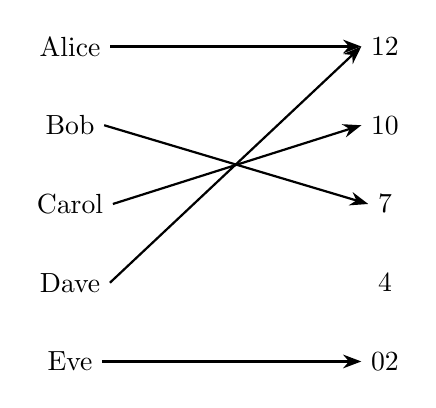
\begin{tikzpicture}[>=Stealth] % Stealth is a nice arrow style
        % Left column of names
        \node (A1) at (0,0) {Alice};
        \node (A2) at (0,-1) {Bob};
        \node (A3) at (0,-2) {Carol};
        \node (A4) at (0,-3) {Dave};
        \node (A5) at (0,-4) {Eve};
        
        % Right column of numbers
        \node (B1) at (4,0) {$12$};
        \node (B2) at (4,-1) {$10$};
        \node (B3) at (4,-2) {$7$};
        \node (B4) at (4,-3) {$4$};
        \node (B5) at (4,-4) {$02$};
        
        % Connecting lines with arrows
        \draw[->, thick, black] (A1.east) -- (B1.west);
        \draw[->, thick, black] (A2.east) -- (B3.west);
        \draw[->, thick, black] (A3.east) -- (B2.west);
        \draw[->, thick, black] (A4.east) -- (B1.west);
        \draw[->, thick, black] (A5.east) -- (B5.west);
    \end{tikzpicture}
    \caption{Example of a function mapping names to numbers.}
    \label{fig:names_to_numbers}
\end{figure}


This assignment of grades, illustrated in \autoref{fig:names_to_numbers}, exemplifies a function.

Functions play a crucial role in mathematics and computer science. They define discrete structures such as sequences and strings and are used to analyse the time complexity of algorithms. Many computer programs are designed to compute values of functions. Recursive functions, defined in terms of themselves, are especially significant in computer science. This section provides an overview of the fundamental concepts of functions needed in the mathematics for software engineering.

\begin{definition}
Let $A$ and $B$ be nonempty sets. A function $f$ from $A$ to $B$ is an assignment of exactly one element of $B$ to each element of $A$. We write $f(a)=b$ if $b$ is the unique element of $B$ assigned by the function $f$ to the element $a$ of $A$. If $f$ is a function from $A$ to $B$, we write $f: A \rightarrow B$.
\end{definition}

\begin{remark}
    Functions are sometimes also called mappings or transformations.
\end{remark}

Functions can be specified in various ways. Sometimes, we explicitly state the assignments, as shown in \autoref{fig:names_to_numbers}. Often, a formula such as \(f(x) = x + 1\) is used to define a function. In other cases, a computer program may specify the function.

\begin{definition}
If $f$ is a function from $A$ to $B$, we say that $A$ is the \textbf{domain} of $f$ and $B$ is the \textbf{co-domain} of $f$. If $f(a)=b$, we say that $b$ is the \textbf{image} of $a$ and $a$ is a \textbf{preimage} of $b$. The \textbf{range}, or image, of $f$ is the set of all images of elements of $A$. Also, if $f$ is a function from $A$ to $B$, we say that $f$ \textbf{maps} $A$ to $B$.    
\end{definition}

When defining a function, we specify its domain, co-domain, and the mapping of elements from the domain to the co-domain. Two functions are equal if they have the same domain, the same co-domain, and map each element of their domain to the same element in the co-domain. 

It's important to note that altering the domain or co-domain results in a different function. Similarly, changing the mapping of elements also produces a different function.


\begin{figure}[htbp]
\centering
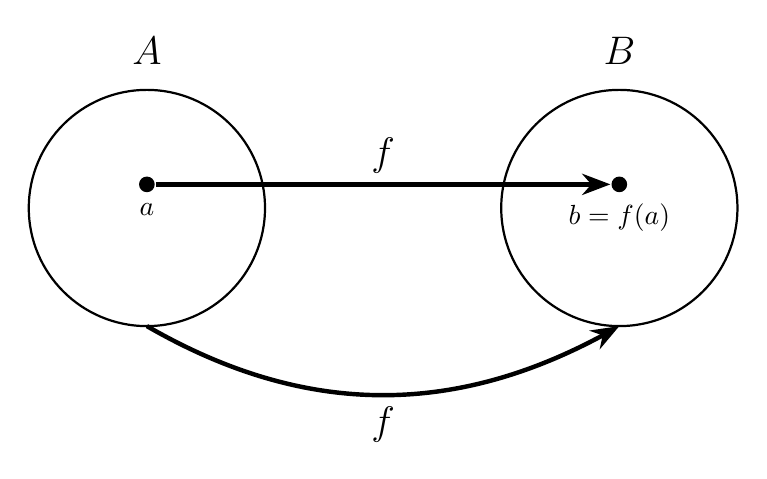
\begin{tikzpicture}[>=Stealth, node distance=4cm, thick, scale=1]

    % Draw larger circles for sets A and B
    \draw[thick] (0,0) circle [radius=1.5cm] node at (0, 2) {\Large $A$};
    \draw[thick] (6,0) circle [radius=1.5cm] node at (6, 2) {\Large $B$};

    % Place larger nodes for elements a and b=f(a)
    \node[fill, circle, inner sep=2pt, label=below:{$a$}] (a) at (0,0.3) {};
    \node[fill, circle, inner sep=2pt, label=below:{$b=f(a)$}] (b) at (6,0.3) {};

    % Draw the larger straight arrow representing f
    \draw[->, ultra thick, black] (a) -- (b) node[midway, above] {\Large $f$};

    % Draw the curved arrow representing f at the bottom, touching the circles
    \draw[->, ultra thick, black, bend right=30] ([shift={(270:1.5cm)}]0,0) 
    to node[midway, below] {\Large $f$} 
    ([shift={(270:1.5cm)}]6,0);

\end{tikzpicture}
\caption{A function \(f\) mapping an element \(a\) from set \(A\) to an element \(b=f(a)\) in set \(B\).}
\label{fig:function_mapping}
\end{figure}

The following examples illustrate various functions. In each example, we describe the domain, co-domain, range, and the assignment of values to the elements of the domain.

\begin{example} What are the domain, co-domain, and range of the function that assigns grades to students described in the first paragraph of the introduction of this section?

\begin{solution}
    Let $G$ be the function that assigns a grade to a student in our Software engineering mathematics class. Note that $G$(Alice) $=12$, for instance. The domain of $G$ is the set \{Alice, Bob, Carol, David, Eve $\}$, and the co-domain is the set $\{12, 10, 7, 4, 02\}$. The range of $G$ is the set $\{12, 10, 7, 02\}$, because each grade except $4$ is assigned to some student.
\end{solution}
    
\end{example}

\begin{example}
    Let $f$ be the function that assigns the last two bits of a bit string of length 2 or greater to that string. For example, $f(11010)=10$. Then, the domain of $f$ is the set of all bit strings of length 2 or greater, and both the co-domain and range are the set $\{00,01,10,11\}$.
\end{example}

\begin{example}
    Let $f: \mathbb{Z} \rightarrow \mathbb{Z}$ assign the square of an integer to this integer. Then, $f(x)=x^2$, where the domain of $f$ is the set of all integers, the co-domain of $f$ is the set of all integers, and the range of $f$ is the set of all integers that are perfect squares, namely, $\{0,1,4,9, \ldots\}$.
\end{example}

\subsection*{One-to-One and Onto Functions}
In mathematics, functions are a fundamental concept used to describe the relationship between two sets. However, not all functions behave the same way. To understand these differences, we introduce the concepts of one-to-one (injective) and onto (surjective) functions.

Some functions never assign the same value to two different domain elements. These functions are said to be \textbf{one-to-one}.

\begin{definition} {One-to-One functions (Injective)}
A function \( f: A \rightarrow B \) is called \textbf{one-to-one} (or \textbf{injective}) if different elements in \( A \) map to different elements in \( B \). In other words, if \( f(a_1) = f(a_2) \), then \( a_1 = a_2 \). This property ensures that no two distinct elements in \( A \) are mapped to the same element in \( B \).     
\end{definition}

Graphically, a function is one-to-one if no horizontal line intersects the graph of the function at more than one point.

\begin{definition}{Onto Functions (Surjective)}
A function \( f: A \rightarrow B \) is called \textbf{onto} (or \textbf{surjective}) if every element in \( B \) is the image of at least one element in \( A \). In other words, for every \( b \in B \), there exists at least one \( a \in A \) such that \( f(a) = b \). This property ensures that the function ``covers'' the entire set \( B \).
\end{definition}

\subsection*{Inverse Functions}

Now, consider a function \( f: A \rightarrow B \) that is both one-to-one and onto. Because \( f \) is onto, every element of \( B \) is the image of some element in \( A \). Furthermore, because \( f \) is one-to-one, every element of \( B \) is the image of a unique element of \( A \). This unique correspondence allows us to define a new function from \( B \) to \( A \) that ``reverses'' the mapping given by \( f \).

\begin{figure}[htbp]
\centering
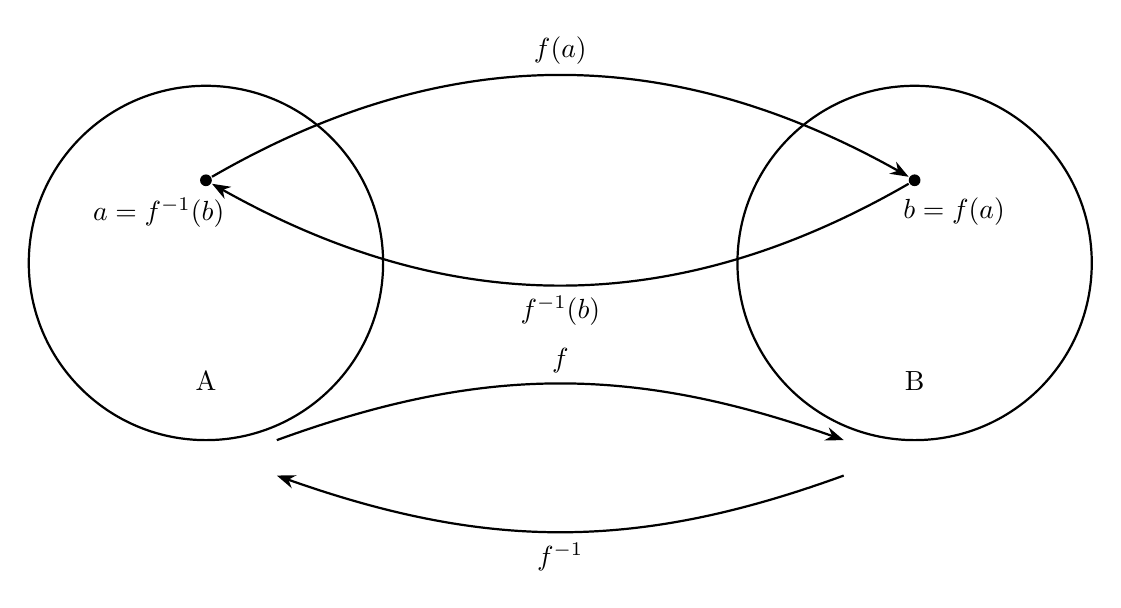
\begin{tikzpicture}[>=Stealth, thick, scale = 1.5]

% Draw circles representing sets A and B
\draw (0,0) circle (1.5cm);
\draw (6,0) circle (1.5cm);

% Labels for sets A and B
\node at (0,-1) {A};
\node at (6,-1) {B};


% Points in sets with adjusted labels
\node[fill=black, circle, inner sep=1.5pt, label={[xshift=-0.6cm]below:{$a = f^{-1}(b)$}}] (A1) at (0,0.7) {};
\node[fill=black, circle, inner sep=1.5pt, label={[xshift=0.5cm]below:{$b = f(a)$}}] (B1) at (6,0.7) {};


% Arrows for f and f^{-1}
\draw[->] (A1) to[bend left=30] node[midway, above] {$f(a)$} (B1);
\draw[->] (B1) to[bend left=30] node[midway, below] {$f^{-1}(b)$} (A1);

% Arrows for f and f^{-1} below the main circles
\draw[->] (0.6,-1.5) to[bend left=20] node[midway, above] {$f$} (5.4,-1.5);
\draw[->] (5.4,-1.8) to[bend left=20] node[midway, below] {$f^{-1}$} (0.6,-1.8);

\end{tikzpicture}
\caption{The function $f^{-1}$ is the inverse of function $f$.}
\label{fig:inv}
\end{figure}

This new function is called the \textbf{inverse function} of \( f \), denoted by \( f^{-1}: B \rightarrow A \). The inverse function \( f^{-1} \) satisfies the following properties:

\[
f(f^{-1}(b)) = b \quad \text{for every } b \in B.
\]
\[
f^{-1}(f(a)) = a \quad \text{for every } a \in A.
\]

We can summarise these considerations in the following definition

\begin{definition}{Inverse Functions}
Let $f$ be a one-to-one correspondence from the set $A$ to the set $B$. The inverse function of $f$ is the function that assigns to an element $b$ belonging to $B$ the unique element $a$ in $A$ such that $f(a)=b$. The inverse function of $f$ is denoted by $f^{-1}$. Hence, $f^{-1}(b)=a$ when $f(a)=b$.    
\end{definition}

These properties show that \( f^{-1} \) effectively undoes the work of \( f \), mapping each element of \( B \) back to the corresponding element in \( A \).

\begin{example}


Let \( f: \mathbb{R} \rightarrow \mathbb{R} \) be defined by \( f(x) = 2x + 3 \). We can check that \( f \) is both one-to-one and onto:

\begin{itemize}
    \item \textbf{One-to-One}: If \( f(x_1) = f(x_2) \), then \( 2x_1 + 3 = 2x_2 + 3 \). Subtracting 3 from both sides gives \( 2x_1 = 2x_2 \), and dividing by 2 yields \( x_1 = x_2 \). Thus, \( f \) is one-to-one.
    \item \textbf{Onto}: Given any \( y \in \mathbb{R} \), we can solve \( y = 2x + 3 \) for \( x \) to find \( x = \frac{y - 3}{2} \). Since this \( x \) exists for every \( y \), \( f \) is onto.
\end{itemize}

Since \( f \) is both one-to-one and onto, it has an inverse function \( f^{-1} \) defined by

\[
f^{-1}(y) = \frac{y - 3}{2}.
\]

  
\end{example}

\subsection*{Composite Functions}
In mathematics, functions can be combined to form new functions. One important way of combining functions is through the composition of functions. The composite of two functions is essentially applying one function to the results of another.

\begin{figure}[htbp]
\centering
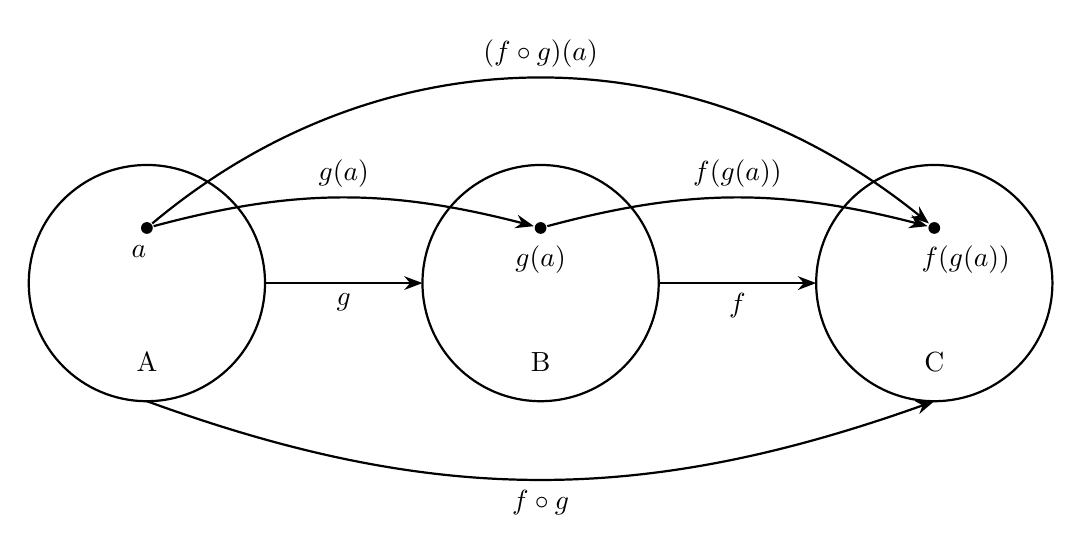
\begin{tikzpicture}[>=Stealth, thick]

% Draw circles representing sets A, B, and C
\draw (0,0) circle (1.5cm);  % Set A
\draw (5,0) circle (1.5cm);  % Set B
\draw (10,0) circle (1.5cm); % Set C

% Labels for sets A, B, and C
\node at (0,-1) {A};
\node at (5,-1) {B};
\node at (10,-1) {C};

% Points in sets with adjusted labels
\node[fill=black, circle, inner sep=1.5pt, label={[xshift=-0.1cm]below:{$a$}}] (A) at (0,0.7) {};

\node[fill=black, circle, inner sep=1.5pt, label=below:{$g(a)$}] (B) at (5,0.7) {};
\node[fill=black, circle, inner sep=1.5pt, label={[xshift=0.4cm]below:{$f(g(a))$}}] (C) at (10,0.7) {};

% Arrows for g and f
\draw[->] (A) to[bend left=15] node[midway, above] {$g(a)$} (B);
\draw[->] (B) to[bend left=15] node[midway, above] {$f(g(a))$} (C);
\draw[->] ([shift={(360:1.5cm)}]0,0) to node[midway, below] {$g$} (3.5,0);
\draw[->] ([shift={(360:0cm)}]6.5,0) to node[midway, below] {$f$} (8.5,0);

% Arrows for f ∘ g and (f ∘ g)(a)
\draw[->] (A) to[bend left=40] node[midway, above] {$(f \circ g)(a)$} (C);
% Draw the curved arrow representing f at the bottom, touching the circles
\draw[->, bend right=20] ([shift={(270:1.5cm)}]0,0) to node[midway, below] {$f \circ g$} ([shift={(270:1.5cm)}]10,0);

\end{tikzpicture}
\caption{The composition of $f$ and $g$.}
\label{fig:composite}
\end{figure}

\begin{definition}
    

Let \( f: B \rightarrow C \) and \( g: A \rightarrow B \) be two functions. The \textbf{composite function} of \( f \) and \( g \), denoted by \( f \circ g \), is a function from \( A \) to \( C \) defined by

\[
(f \circ g)(x) = f(g(x)),
\]

for every \( x \in A \).

\end{definition}

In other words, the composite function \( f \circ g \) means that you first apply the function \( g \) to the input \( x \), and then apply the function \( f \) to the result of \( g(x) \). In \autoref{fig:composite} the composition of functions is shown.

\begin{example}
    

Consider the functions \( f(x) = 2x + 3 \) and \( g(x) = x^2 \). The composite function \( f \circ g \) is given by:

\[
(f \circ g)(x) = f(g(x)) = f(x^2) = 2x^2 + 3.
\]

Here, the function \( g(x) \) squares the input \( x \), and then the function \( f(x) \) multiplies the result by 2 and adds 3.
\end{example}

Now, let's reverse the composition and compute \( g \circ f \):

\[
(g \circ f)(x) = g(f(x)) = g(2x + 3) = (2x + 3)^2.
\]

Notice that \( f \circ g \) and \( g \circ f \) are generally different functions, illustrating that the composition of functions is not commutative.

\begin{example}
    Let $g$ be the function from the set $\{a, b, c\}$ to itself such that $g(a)=b, g(b)=c$, and $g(c)=a$. Let $f$ be the function from the set $\{a, b, c\}$ to the set $\{1,2,3\}$ such that $f(a)=3, f(b)=2$, and $f(c)=1$. What is the composition of $f$ and $g$, and what is the composition of $g$ and $f$ ?

    \begin{solution}
        The composition $f \circ g$ is defined by $(f \circ g)(a)=f(g(a))=f(b)=2$, $(f \circ g)(b)=f(g(b))=f(c)=1$, and $(f \circ g)(c)=f(g(c))=f(a)=3$.
        
        Note that $g \circ f$ is not defined, because the range of $f$ is not a subset of the domain of $g$.
    \end{solution}
\end{example}


\begin{example}{label:}
Let $f$ and $g$ be the functions from the set of integers to the set of integers defined by $f(x)=2 x+3$ and $g(x)=3 x+2$. What is the composition of $f$ and $g$ ? What is the composition of $g$ and $f$?

\begin{solution}
Both the compositions $f \circ g$ and $g \circ f$ are defined. Moreover,
\[
(f \circ g)(x)=f(g(x))=f(3 x+2)=2(3 x+2)+3=6 x+7
\]
and
\[
(g \circ f)(x)=g(f(x))=g(2 x+3)=3(2 x+3)+2=6 x+11 .
\]
\end{solution}
\end{example}

\begin{remark}
Even though \( f \circ g \) and \( g \circ f \) are defined for the functions \( f \) and \( g \) in example 35, \( f \circ g \) and \( g \circ f \) are not equal. In other words, the commutative law does not hold for the composition of functions.
  
\end{remark}

When the composition of a function and its inverse is formed, in either order, an identity function is obtained. To see this, suppose that \( f \) is a one-to-one correspondence from the set \( A \) to the set \( B \). Then the inverse function \( f^{-1} \) exists and is a one-to-one correspondence from \( B \) to \( A \). The inverse function reverses the correspondence of the original function, so \( f^{-1}(b)=a \) when \( f(a)=b \), and \( f(a)=b \) when \( f^{-1}(b)=a \).

Hence,

\[
\left(f^{-1} \circ f\right)(a) = f^{-1}(f(a)) = f^{-1}(b) = a,
\]

and

\[
\left(f \circ f^{-1}\right)(b) = f\left(f^{-1}(b)\right) = f(a) = b.
\]

Consequently, \( f^{-1} \circ f = I_A \) and \( f \circ f^{-1} = I_B \), where \( I_A \) and \( I_B \) are the identity functions on the sets \( A \) and \( B \), respectively. That is, \( \left(f^{-1}\right)^{-1} = f \).

\begin{example}
    If $f: \mathbb{R} \rightarrow \mathbb{R}$ is defined as $f(x)=2 x+3$, then $f^{-1}(x)=\frac{x-3}{2}$. The composition $f \circ f^{-1}$ would be the identity function $I_{\mathbb{R}}$ on the real numbers, meaning $f\left(f^{-1}(x)\right)=x$ for all $x \in \mathbb{R}$.
\end{example}

\section{Graphical Identification of Function Types}
Understanding the behaviour of different types of functions is fundamental in mathematics. Functions can be classified based on their graphical patterns, which provide valuable insights into their characteristics. In this section, we will explore various types of functions, including linear, quadratic, exponential, and more. By examining their graphs, we can identify key features such as intercepts, slopes, curvature, and asymptotic behaviour, enabling us to distinguish between these different types of functions effectively.

\subsection*{Linear Functions}
The general equation for a linear function is given by

\[
y = ax + b \quad \text{(often written as } y = mx + b\text{)},
\]

where \(a\) (or \(m\)) represents the slope and \(b\) is the y-intercept. The domain of this function is all real numbers. This equation is in slope-intercept form because \(a\) (or \(m\)) gives the slope and \(b\) gives the y-intercept. If \(a = 0\), the function simplifies to \(y = b\), which is a constant function.

The parent function for a linear equation is

\[
y = x.
\]

The transformed function can be written in the point-slope form as

\[
y = y_1 + a(x - x_1),
\]

where the graph contains the point \((x_1, y_1)\) and has slope \(a\). In this form:
\begin{itemize}
    \item \(a\) is the vertical dilation (slope),
    \item \(y_1\) represents the vertical translation,
    \item \(x_1\) represents the horizontal translation.
\end{itemize}

This point-slope form can also be written as

\[
y - y_1 = a(x - x_1),
\]

where the coordinates of the fixed point \((x_1, y_1)\) appear with a negative sign. The form \(y = y_1 + a(x - x_1)\) expresses \(y\) explicitly in terms of \(x\), making it easier to enter into a graphing calculator.

\begin{figure}[htbp]
    \centering
    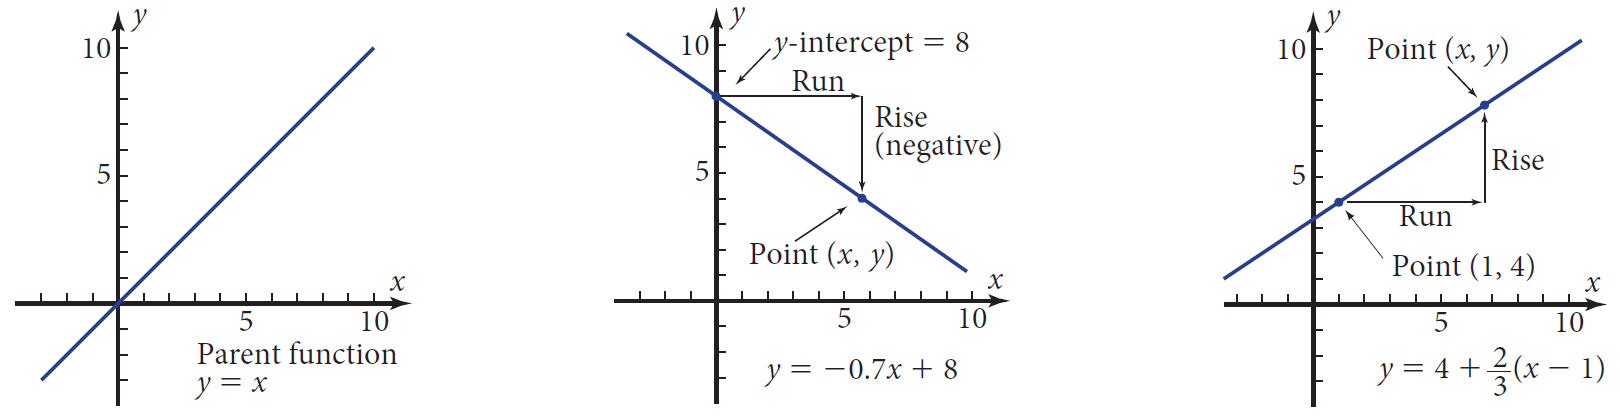
\includegraphics[width=1\textwidth]{figure/book1.png} % Adjust width here to scale the image
    \caption{Linear functions}
    \label{fig:book_image}
\end{figure}

The graph of a linear function is a straight line. The parent function \(y = x\) is shown on the left in \autoref{fig:book_image}, the slope-intercept form in the middle, and the point-slope form on the right.

For the slope-intercept form: "Start at \(b\) on the \(y\)-axis, move \(x\) units horizontally, and rise \(ax\) units vertically." For the point-slope form: "Start at \((x_1, y_1)\), move \((x - x_1)\) units horizontally, and rise \(a(x - x_1)\) units vertically."

\subsection*{Quadratic Functions}
The general equation for a quadratic function is given by

\[
y = ax^2 + bx + c,
\]

where \(a \neq 0\), and \(a\), \(b\), and \(c\) are constants. The domain of this function is all real numbers.

\begin{figure}[htbp]
    \centering
    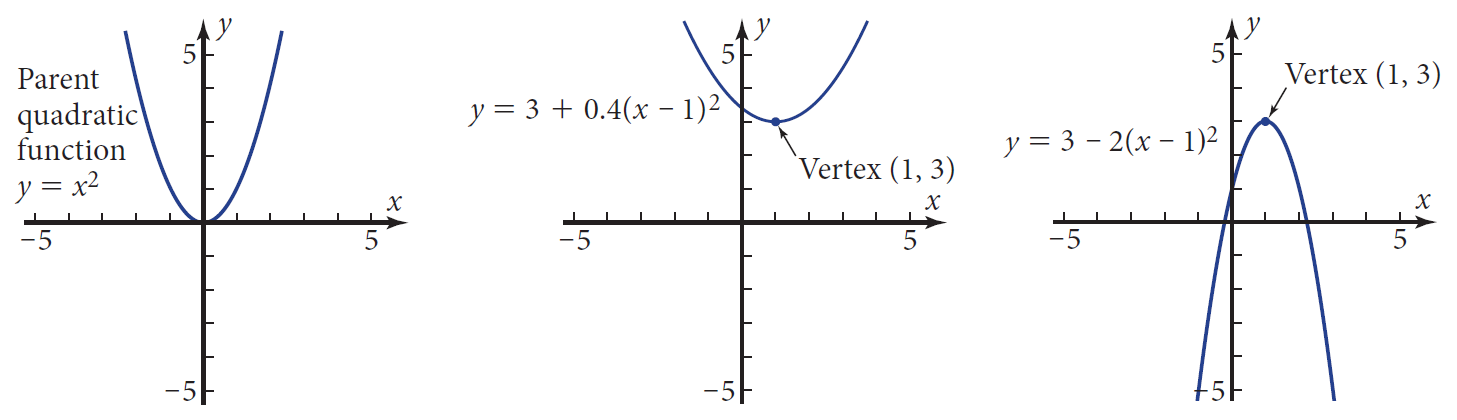
\includegraphics[width=1\textwidth]{figure/book2.png} % Adjust width here to scale the image
    \caption{Quadratic functions}
    \label{fig:book_image2}
\end{figure}

The parent function for a quadratic equation is

\[
y = x^2,
\]

where the vertex of the parabola is at the origin \((0, 0)\).

The transformed function can be written in vertex form as

\[
y = k + a(x-h)^2,
\]

where the vertex of the parabola is located at \((h, k)\). In this form:
\begin{itemize}
    \item \(k\) represents the vertical translation,
    \item \(h\) represents the horizontal translation,
    \item \(a\) represents the vertical dilation.
\end{itemize}

Vertex form can also be written as

\[
y - k = a(x-h)^2,
\]

but expressing \(y\) explicitly in terms of \(x\) makes the equation easier to enter into a graphing calculator.

The graph of a quadratic function is a parabola (from the Greek word for "along the path of a ball"). The parabola is concave up if \(a > 0\) and concave down if \(a < 0\). This behaviour is illustrated in \autoref{fig:book_image2}.

\subsection*{Power Functions}
The general equation for a power function is given by

\[
y = ax^b,
\]

where \(a\) and \(b\) are nonzero constants. The domain of the function depends on the value of \(b\):
\begin{itemize}
    \item If \(b > 0\), the domain is all real numbers.
    \item If \(b < 0\), the domain excludes \(x = 0\) to avoid division by zero.
    \item If \(b\) is not an integer, the domain usually excludes negative numbers to avoid taking roots of negative numbers.
\end{itemize}
In most applications, the domain is restricted to non-negative numbers.

\begin{figure}[htbp]
    \centering
    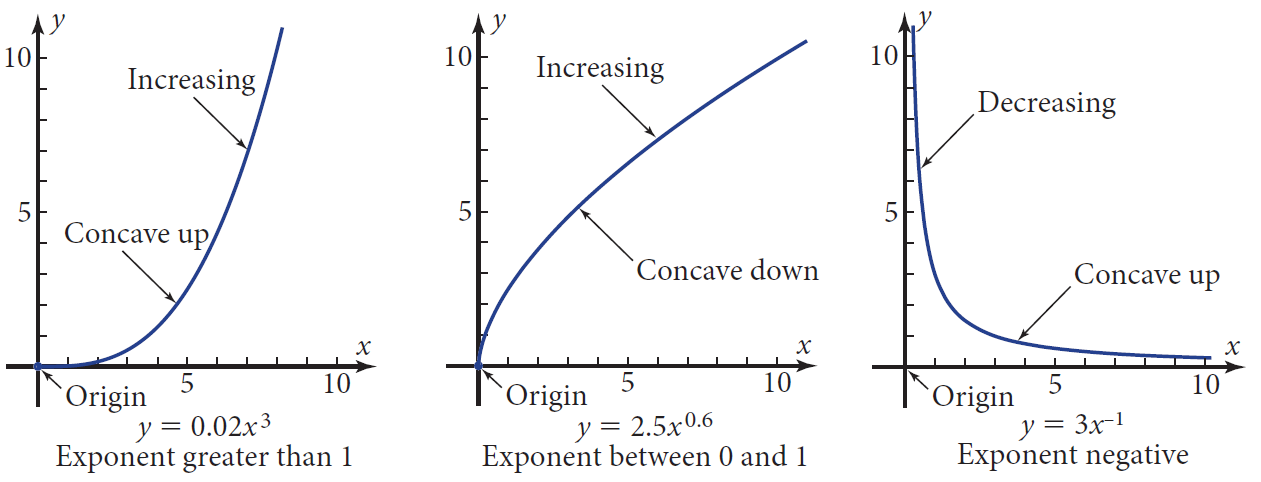
\includegraphics[width=1\textwidth]{figure/book3.png} % Adjust width here to scale the image
    \caption{Power functions}
    \label{fig:book_image3}
\end{figure}

The parent function for a power function is

\[
y = x^b.
\]

For the general power function \(y = ax^b\):
\begin{itemize}
    \item If \(b > 0\), then \(y\) varies directly with the \(b\)th power of \(x\), meaning \(y\) is directly proportional to the \(b\)th power of \(x\).
    \item If \(b < 0\), then \(y\) varies inversely with the \(b\)th power of \(x\), meaning \(y\) is inversely proportional to the \(b\)th power of \(x\).
\end{itemize}

The dilation factor \(a\) serves as the proportionality constant.

The translated form of a power function is

\[
y = d + a(x - c)^b,
\]

where \(c\) and \(d\) are the horizontal and vertical translations, respectively. This can be compared with the translated forms of linear and quadratic functions:

\[
\begin{aligned}
& y = y_1 + a(x - x_1) &\text{(linear function)}, \\
& y = k + a(x - h)^2 &\text{(quadratic function)}.
\end{aligned}
\]

Unless otherwise stated, "power function" will imply the untranslated form, \(y = ax^b\).

\autoref{fig:book_image3} shows the graphs of power functions for different values of \(b\). In all cases, \(a > 0\). The shape and concavity of the graph depend on the value of \(b\):
\begin{itemize}
    \item If \(b > 0\), the graph contains the origin.
    \item If \(b < 0\), the graph has the axes as asymptotes.
    \item The function is increasing if \(b > 0\) and decreasing if \(b < 0\).
    \item The graph is concave up if \(b > 1\) or \(b < 0\), and concave down if \(0 < b < 1\).
\end{itemize}
The concavity of the graph describes the rate at which \(y\) increases. For \(b > 0\), concave up indicates that \(y\) is increasing at an increasing rate, while concave down indicates that \(y\) is increasing at a decreasing rate.

\subsection*{Exponential Functions}

The general equation for an exponential function is given by

\[
y = a b^x,
\]

where \(a\) and \(b\) are constants, \(a \neq 0\), \(b > 0\), and \(b \neq 1\). The domain of this function is all real numbers.

The parent function for an exponential equation is

\[
y = b^x,
\]
where the asymptote is the \(x\)-axis.

\begin{figure}[htbp]
    \centering
    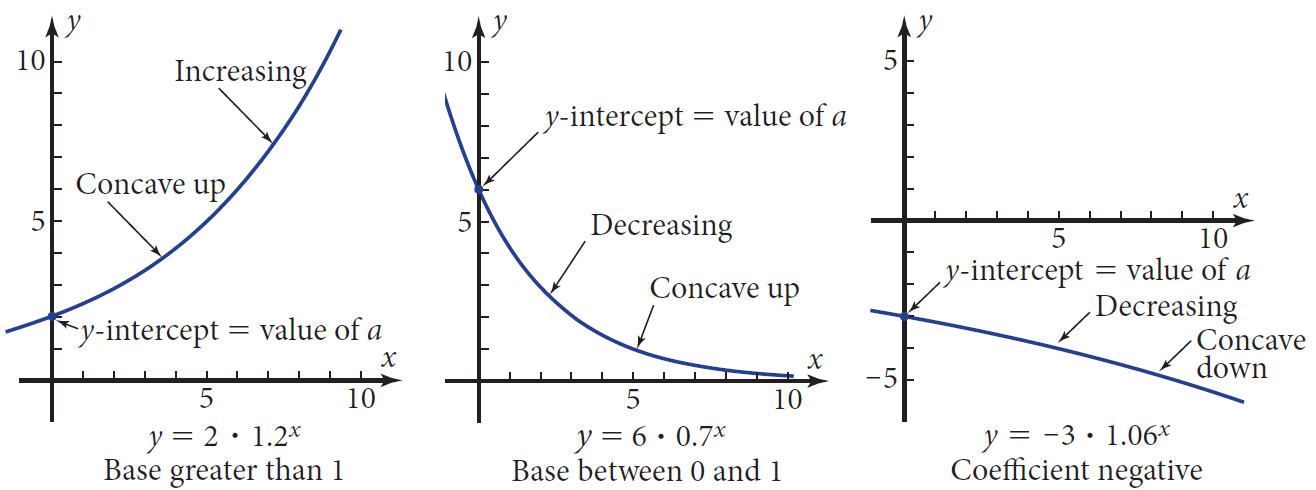
\includegraphics[width=1\textwidth]{figure/book4.png} % Adjust width here to scale the image
    \caption{Exponential functions}
    \label{fig:book_image4}
\end{figure}

In the equation \(y = a b^x\), we say that "\(y\) varies exponentially with \(x\)." This means that \(y\) changes by a constant factor \(b\) for each unit increase in \(x\).

The translated form of the exponential function is

\[
y = a b^x + c,
\]

where the asymptote is the line \(y = c\). Unless otherwise stated, "exponential function" will refer to the untranslated form \(y = a b^x\).

\autoref{fig:book_image4} illustrates exponential functions for different values of \(a\) and \(b\). The key properties of the graph are as follows:
\begin{itemize}
    \item The constant \(a\) is the \(y\)-intercept of the graph.
    \item The function is increasing if \(b > 1\) and decreasing if \(0 < b < 1\), provided \(a > 0\).
    \item If \(a < 0\), the function's behavior is reversed: it is decreasing if \(b > 1\) and increasing if \(0 < b < 1\).
    \item The graph is concave up if \(a > 0\) and concave down if \(a < 0\).
\end{itemize}

Mathematicians often use one of two particular constants as the base for an exponential function: either 10, which is the base of the decimal system, or the naturally occurring number \( e \), which approximately equals 2.71828. These bases are significant in various mathematical applications.

\begin{definition}{Special Exponential Functions}

\begin{align*}
y &= a \cdot 10^{bx} \hspace{1cm} \text{base-10 exponential function} \\
y &= a \cdot e^{bx}  \hspace{1.2cm} \text{natural (base-}e\text{) exponential function,}
\end{align*}

where $a$ and $b$ are constants and the domain is all real numbers.
    
\end{definition}

To generalise the exponential function, the variable in the exponent is often multiplied by a constant. The (untranslated) general forms of these exponential functions are given below:

\[
y = a \cdot 10^{bx}
\quad \text{and} \quad
y = a \cdot e^{bx}
\]

These functions can be further generalised by incorporating translations in both the \(x\)- and \(y\)-directions. The translated forms are:

\[
y = a \cdot 10^{b(x - c)} + d
\quad \text{and} \quad
y = a \cdot e^{b(x - c)} + d
\]

The base-\(e\) exponential function, in particular, has a significant advantage when studying calculus, as the rate of change of \(e^x\) is equal to \(e^x\) itself.

\section{Logarithms}
Any positive number can be written as a power of 10. For instance,

\[
\begin{aligned}
3 & = 10^{0.477 \ldots} \\
5 & = 10^{0.6989 \ldots} \\
15 & = 10^{1.1760 \ldots}
\end{aligned}
\]

The exponents \(0.4771 \ldots\), \(0.6989 \ldots\), and \(1.1760 \ldots\) are called the base-10 logarithms of 3, 5, and 15, respectively:

\[
\begin{aligned}
\log 3 & = 0.4771 \ldots \\
\log 5 & = 0.6989 \ldots \\
\log 15 & = 1.1760 \ldots
\end{aligned}
\]

To better understand the meaning of logarithms, press \texttt{LOG} 3 on your calculator. You will get:

\[
\log 3 = 0.477121254 \ldots
\]

Then, without rounding, raise 10 to this power. You will obtain:

\[
10^{0.477121254 \ldots} = 3
\]

The powers of 10 have the normal properties of exponentiation. For instance,
\[
\begin{aligned}
15 & = (3)(5) = \left(10^{0.4771 \ldots}\right)\left(10^{0.6999 \ldots}\right) \\
& = 10^{0.4771 \ldots + 0.6599 \ldots} \\
& = 10^{1.1760 \ldots}
\end{aligned}
\]

This means \(10^{0.4771 \ldots + 0.6599 \ldots} = 10^{1.1760 \ldots}\). Here, you add the exponents while keeping the same base. You can verify with your calculator that \(10^{1.1760 \ldots}\) indeed equals 15.

From this example, you can infer that logarithms have the same properties as exponents. This is expected because logarithms \textit{are} exponents. For instance,

\[
\log(3 \cdot 5) = \log 3 + \log 5 \quad \text{\textit{The logarithm of a product equals the sum of the logarithms of the factors}.}
\]

From the values given earlier, you can also show that:

\[
\log \frac{15}{3} = \log 15 - \log 3 \quad \text{\textit{The logarithm of a quotient}.}
\]

This property is reasonable because you divide powers of equal bases by subtracting the exponents:

\[
\frac{15}{3} = \frac{10^{1.1760 \ldots}}{10^{0.477 \ldots}} = 10^{1.1760 \ldots - 0.4771 \ldots} = 10^{0.6989 \ldots} = 5
\]

Since a power can be written as a product, you can find the logarithm of a power as follows:

\[
\begin{aligned}
\log 34 & = \log (3 \cdot 3 \cdot 3 \cdot 3) = \log 3 + \log 3 + \log 3 + \log 3 \\
& = 4 \log 3 \quad \text{\textit{Combine like terms}.}
\end{aligned}
\]

The logarithm of a power equals the exponent of that power times the logarithm of the base. To verify this result, observe that \(3^4 = 81\). Press \(4 \times \texttt{LOG}\,3\) on your calculator, and you'll find it equals \(1.9084 \ldots\).

\begin{definition}{Base-10 Logarithms}

\[
\log x=y \iff 10^y=x
\]

\textit{Verbally}: $\log x$ is the exponent in the power of 10 that gives $x$   
\end{definition}

The term logarithm comes from the Greek words \emph{logos}, meaning "ratio," and \emph{arithmos}, meaning "number." Before the invention of calculators, base-10 logarithms were calculated approximately using infinite series and recorded in tables. Products involving many factors, such as
\[
(357)(4.367)(22.4)(3.142)
\]
could be calculated by adding their logarithms (exponents) rather than tediously multiplying several pairs of numbers. This method was invented by Englishman Henry Briggs (1561–1630) and Scotsman John Napier (1550–1616). The name logarithm, thus, reflects this "logical way to do arithmetic".

\begin{custombox}{Properties of base-10 logarithms}
\begin{itemize}
    \item Log of a Product:
    
    \[
    \log x y=\log x+\log y
    \]
    
    \textit{Verbally}: The $\log$ of a product equals the sum of the logs of the factors.
    \vspace{0.2cm}
    \item Log of a Quotient:
    
    \[
    \log \frac{x}{y}=\log x-\log y
    \]
    \vspace{0.1cm}
    \textit{Verbally}: The $\log$ of a quotient equals the log of the numerator minus the $\log$ of the denominator.
    \vspace{0.2cm}
    \item Log of a Power:
    \[
    \log x^y=y \log x
    \]
    \textit{Verbally}: The $\log$ of a power equals the exponent times the log of the base.
\end{itemize}

   
\end{custombox}

\begin{example} Find $x$ if $\log_{10} 10^{3.721}=x$

\begin{solution}
By definition, the logarithm is the exponent of 10. So $x=3.721$.
\end{solution}
\end{example}

\begin{example} Find $x$ if $0.258=10^x$

\begin{solution}
   By definition, $x$, the exponent of 10, is the logarithm of 0.258.

    \[
    x=\log_{10} 0.258=-0.5883 \ldots
    \]
\end{solution}
    
\end{example}

\begin{custombox}{The most important thing to remember about logarithms is this}
    \textbf{A logarithm is an exponent.}
\end{custombox}

\subsection*{Logarithms with Any Base: The Change-of-Base Property}
If \(x = 10^y\), then \(y\) is the base-10 logarithm of \(x\). Similarly, if \(x = 2^y\), then \(y\) is the base-2 logarithm of \(x\). The only difference between these logarithms is the number that serves as the base. To distinguish among logarithms with different bases, the base is written as a subscript after the abbreviation "log." For instance:

\[
\begin{aligned}
3 &= \log_2 8 \Leftrightarrow 2^3 = 8, \\
4 &= \log_3 81 \Leftrightarrow 3^4 = 81, \\
2 &= \log_{10} 100 \Leftrightarrow 10^2 = 100.
\end{aligned}
\]

The symbol \(\log_2 8\) is pronounced "log to the base 2 of 8." The symbol \(\log_{10} 100\) is, of course, equivalent to \(\log 100\), as defined in the previous section. Note that in all cases, a logarithm represents an exponent.

\begin{definition}{Logarithm with Any Base}
\textit{Algebraically}:

\hspace{1cm}$\log _b x=y$ if and only if $b^y=x, \quad$ where $b>0, b \neq 1$, and $x>0$

\vspace{0.3cm}

\textit{Verbally}:

\hspace{1cm} $\log _b x=y$ means that $y$ is the exponent of $b$ that gives $x$ as the answer.
    
\end{definition}

The way you pronounce the symbol for logarithm gives you a way to remember the definition. The next two examples show you how to do this.

\begin{example} Write $\log _5 c=a$ in exponential form.

\begin{solution}

Think this:
\begin{itemize}
    \item "\(\log_5 \ldots\)" is read as "log base 5 \(\ldots\)," meaning 5 is the base.
    \item A logarithm is an exponent. Since the \(\log\) equals \(a\), \(a\) must be the exponent.
    \item The "answer" obtained from \(5^a\) is the argument of the logarithm, denoted as \(c\).
\end{itemize}

Write only this: 

\[
5^a = c
\]
\end{solution}
\end{example}

\begin{example} Write $z^4=m$ in logarithmic form.

\begin{solution}
    $\log _z m=4$
\end{solution}
    
\end{example}

Two bases of logarithms are used frequently enough to have their own key on most calculators. One is the base-10 logarithm, also known as the common logarithm, as discussed in the previous section. The other is the base-\(e\) logarithm, known as the natural logarithm, where \(e = 2.71828 \ldots\), a naturally occurring number (like \(\pi\)) that will be advantageous in your future mathematical studies.

The symbol \(\ln x\) (pronounced "el en of \(x\)") is used for natural logarithms, and is defined as:
\[
\ln x = \log_e x
\]

\begin{definition}{Common Logarithm and Natural Logarithm}
\hspace{1cm} \textit{Common}: The symbol $\log x$ means $\log _{10} x$.

\hspace{1cm}  \textit{Natural}: \hspace{0.2cm}The symbol $\ln x$ means $\log _e x$, where $e$ is a constant equal to $2.71828182845 \ldots$
\end{definition}

\begin{example} Find $\log _5 17$. Check your answer by an appropriate numerical method.

\begin{solution} Let $x=\log _5 17$.

\begin{equation*}
\begin{aligned}
& 5^x=17 \\
& \log _{10} 5^x=\log _{10} 17 \\
& x \log _{10} 5=\log _{10} 17 \\
& x=\frac{\log _{10} 17}{\log _{10} 5}=1.7603 \ldots \\
& \log _5 17=1.7603 \ldots \\
& 5^{1.7603 \ldots}=17
\end{aligned}
\end{equation*}
\end{solution}
\end{example}

In this example, note that the base-5 logarithm of a number is directly proportional to the base-10 logarithm of that number. The conclusion of the example can be expressed as follows:

\[
\log_5 17 = \frac{1}{\log_{10} 5} \cdot \log_{10} 17 = 1.4306 \ldots \log_{10} 17
\]

To find the base-5 logarithm of any number, simply multiply its base-10 logarithm by \(1.4306 \ldots\) (that is, divide by \(\log_{10} 5\)).

This proportional relationship is known as the change-of-base property. From the results of Example 3, you can write:

\[
\log_5 17 = \frac{\log_{10} 17}{\log_{10} 5}
\]

Notice that the logarithm with the desired base is isolated on the left side of the equation, while the two logarithms on the right side share the same base—typically one that is available on your calculator. The box below illustrates this property for bases \(a\) and \(b\) with argument \(x\):

\begin{custombox}{The Change-of-Base Property of Logarithms}

\begin{equation*}
\log _a x=\frac{\log_b x}{\log_b a} \quad \text { or } \quad \log_a x=\frac{1}{\log_b a}\left(\log_b x\right)
\end{equation*}
    
\end{custombox}

\begin{example}
Find $\ln 29$ using the change-of-base property with base-10 logarithms. Check your answer directly by pressing $\ln 29$ on your calculator.

\begin{solution}

\[
\ln 29=\frac{\log 29}{\log e}=\frac{1.4623 \ldots}{0.4342 \ldots}=3.3672 \ldots
\]

\hspace{0.9cm} Directly: $\quad \ln 29=3.3672 \ldots,$

which agrees with the answer we got using the change-of-base property.
\end{solution}
\end{example}

\begin{custombox}{Properties of Logarithms}
\setlength{\leftskip}{1cm}  % Reset the text indent
\setlength{\rightskip}{1cm} % Reset the right indent
The Logarithm of a Power:
$$
\log _b x^y=y \log _b x
$$

\textit{Verbally}: The logarithm of a power equals the product of the exponent and the logarithm of the base.
\vspace{0.5cm}
The Logarithm of a Product:
$$
\log _b(x y)=\log _b x+\log _b y
$$
\textit{Verbally}: The logarithm of a product equals the sum of the logarithms of the factors.
\vspace{0.5cm}
The Logarithm of a Quotient:
$$
\log _b \frac{x}{y}=\log _b x-\log _b y
$$

\textit{Verbally}: The logarithm of a quotient equals the logarithm of the numerator minus the logarithm of the denominator.

\setlength{\leftskip}{0cm}  % Reset the text indent
\setlength{\rightskip}{0cm} % Reset the right indent

\end{custombox}

\subsection*{Solving Exponential and Logarithmic Equations}
Logarithms provide a way to solve an equation with a variable in the exponent or to solve an equation that already contains logarithms. We will demonstrate this through the next few examples.

\begin{example} Solve the exponential equation $7^{3 x}=983$ algebraically, using logarithms.

\begin{solution}
\begin{align*}
& 7^{3x} = 983  \\
& \log 7^{3x} = \log 983 && \texttt{\small Take the base-10 logarithm of both sides.} \\
& 3x \log 7 = \log 983 && \texttt{\small Apply the logarithm power property.} \\
& x = \frac{\log 983}{3 \log 7} && \texttt{\small Divide both sides by the coefficient of x.}\\
& x = 1.1803 \ldots   
\end{align*}


\end{solution}
    
\end{example}

\begin{example} Solve the equation
    \begin{equation*}
\log _2(x-1)+\log _2(x-3)=3
\end{equation*}

\newpage

\begin{solution}

\begin{align*}
& \log _2(x-1)+\log _2(x-3)=3  \\
& \log _2[(x-1)(x-3)]=3 && \texttt{\small Apply the logarithm of a product property.} \\
& 2^3=(x-1)(x-3) && \texttt{\small Use the definition of logarithm.} \\
& 8=x^2-4 x+3 && \texttt{\small Expand the product.}\\
& x^2-4 x-5=0 && \texttt{\small Reduce one side to zero. Use the symmetric }\\
&\vspace{-0.2cm}   && \texttt{\small property of equality.} \\
& (x-5)(x+1)=0 && \texttt{\small Solve by factoring.} \\
& x=5 \quad \text{ or } \quad x=-1
\end{align*}
We need to be cautious here because the solutions in the final step are the solutions of the quadratic equation, and we must make sure they are also solutions of the original logarithmic equation. Check by substituting the solutions into the original equation.

\begin{minipage}[t]{0.45\textwidth}
If $x=5$, then
\[
\begin{aligned}
& \log _2(5-1)+\log _2(5-3) \\
& =\log _2 4+\log _2 2 \\
& =2+1=3
\end{aligned}
\]
\end{minipage}%
\hfill
\begin{minipage}[t]{0.45\textwidth}
If $x=-1$, then
\[
\begin{aligned}
& \log _2(-1-1)+\log _2(-1-3) \\
& =\log _2(-2)+\log _2(-4)
\end{aligned}
\]
which is undefined.
\end{minipage}

\end{solution}

\end{example}

\begin{example} Solve the equation

\[
e^{2 x}-3 e^x+2=0
\]

\begin{solution}

\[
\begin{aligned}
& e^{2 x}-3 e^x+2=0 \\
& \left(e^x\right)^2-3 e^x+2=0
\end{aligned}
\]
We realise that this is a quadratic equation in the variable $e^x$. Using the quadratic formula, you get

\[
\begin{aligned}
& e^x=\frac{+3 \pm \sqrt{9-4(2)}}{2}=\frac{3 \pm 1}{2} \\
& e^x=2 \text { or } e^x=1
\end{aligned}
\]


You now have to solve these two equations.
\[
\begin{array}{ll}
e^x=2 & \qquad e^x=1 \\
x=\ln 2=0.6931 \ldots & \qquad x=0
\end{array}
\]
Check:

\[
\begin{array}{ll}
e^{2 \ln 2}-3 e^{\ln 2}+2 & \qquad \left(e^0\right)^2-3 e^0+2 \\
=\left(e^{\ln 2}\right)^2-3 e^{\ln 2}+2 & \qquad =1^2-3(1)+2=0 \\
=2^2-3(2)+2=0 &
\end{array}
\]
Both solutions are correct.
\end{solution}  
\end{example}

\newpage

\begin{example} Solve the logarithmic equation $\ln (x+3)+\ln (x+5)=0$

\begin{solution}
    \[
\begin{aligned}
& \ln (x+3)+\ln (x+5)=0 \\
& \ln [(x+3)(x+5)]=0 \\
& (x+3)(x+5)=e^0=1 \\
& x^2+8 x+15=1 \\
& x^2+8 x+14=0 \\
& x=-2.5857 \ldots \quad \text { or } \qquad x=-5.4142 \ldots
\end{aligned}
\]
Check:
\[
\begin{aligned}
& x=-2.5857 \ldots: \\
& \ln (-2.5857 \ldots+3)+\ln (-2.5857 \ldots+5) \\
& =\ln (0.4142 \ldots)+\ln (2.4142 \ldots) \\
& =-0.8813 \ldots+0.8813 \ldots=0
\end{aligned}
\]
which is ok.

\[
\begin{aligned}
& x=-5.4142 \ldots: \\
& \ln (-5.4142 \ldots+3)+\ln (-5.4142 \ldots+5) \\
& =\ln (-2.4142 \ldots)+\ln (-0.4142 \ldots)
\end{aligned}
\]

which is undefined.

The only valid solution is $x=-2.5857 \ldots$.
\end{solution}
    
\end{example}



\chapter{Number Systems}
\label{chap:ch2}

We are so accustomed to working within the decimal system that we often forget it is a relatively recent invention and was once considered revolutionary. It is time to carefully examine how we represent numbers. Typically, we use the decimal system, where a number like 3459 is shorthand for \(3 \times 1000 + 4 \times 100 + 5 \times 10 + 9\). The position of each digit is crucial, as it allows us to distinguish between values like 30 and 3. The decimal system is a\textbf{ positional numeral system}, meaning it has designated positions for units, tens, hundreds, and so forth. Each digit’s position implies the multiplier (a power of ten) that should be used with that digit, and each position has a value ten times that of the position to its right.

Notice that we can save space by writing 1000 as \(10^3\), where the exponent 3 indicates the number of zeros. Thus, \(100000 = 10^5\). If the exponent is negative, it represents a fraction, e.g., \(10^{-3} = \frac{1}{1000}\). Perhaps the most ingenious aspect of the positional system was the addition of the decimal point, which allows us to include decimal fractions. For example, the number 123.456 is equivalent to:
\[
1 \times 100 + 2 \times 10 + 3 \times 1 + 4 \times \frac{1}{10} + 5 \times \frac{1}{100} + 6 \times \frac{1}{1000}.
\]

This can be visualised as:
\[
\begin{array}{rccccccccc}
\text{Multiplier:} & \ldots & 10^2 & 10^1 & 10^0 & . & 10^{-1} & 10^{-2} & 10^{-3} & \ldots \\
\text{Digits:} & \ldots & 1 & 2 & 3 & . & 4 & 5 & 6 &\ldots \\
& & & & & \uparrow & & & & \\
& & & & & \text{Decimal Point:} & & & &
\end{array}
\]
However, there is no inherent reason why we must use powers of 10, or base 10. The Babylonians, for instance, used base 60, and base 12 was very common in medieval Europe. Today, the most widely used numeral systems are summarised in \autoref{tab:number_systems}

\begin{table}[ht]
\centering
\renewcommand{\arraystretch}{1.4}
\begin{tabular}{|c|c|c|c|}
\hline
\textbf{Numeral system} & \textbf{Symbols} & \textbf{Base} & \textbf{Additional information} \\ \hline
\textbf{Decimal} & 0-9 & 10 & - \\ \hline
\textbf{Binary} & 0, 1 & 2 & - \\ \hline
\textbf{Hexadecimal} & 0-9, A-F & 16 & $\mathrm{A} \equiv 10, \mathrm{B} \equiv 11, \mathrm{C} \equiv 12,$ $\mathrm{D} \equiv 13, \mathrm{E} \equiv 14, \mathrm{F} \equiv 15$ \\ \hline
\textbf{Octal} & 0-7 & 8 & - \\ \hline
\end{tabular}
\caption{Summary of Common Numeral Systems}
\label{tab:number_systems}
\end{table}

We begin by focusing on binary which will also receive the most detailed attention in this chapter.

\section{Binary Numbers}
In the binary scale, we express numbers in powers of 2 rather than the 10s of the decimal scale. For some numbers, this is easy. Recall $2^0=1$,

\begin{table}[!ht]
\centering
\renewcommand{\arraystretch}{1.4}
\begin{tabular}{|c c c c c c c c|}
\hline 
\multirow{2}{*}{Decimal number} & & \multirow{2}{*}{In powers of 2} & \multicolumn{4}{c}{Power of 2} & \multirow{2}{*}{Binary number} \\
& & & 3 & 2 & 1 & 0 & \\ \hline
8 & $=$ & $2^3$ & 1 & 0 & 0 & 0 & 1000 \\
7 & $=$ & $2^2 + 2^1 + 2^0$ & 0 & 1 & 1 & 1 & 111 \\
6 & $=$ & $2^2 + 2^1$ & 0 & 1 & 1 & 0 & 110 \\
5 & $=$ & $2^2 + 2^0$ & 0 & 1 & 0 & 1 & 101 \\
4 & $=$ & $2^2$ & 0 & 1 & 0 & 0 & 100 \\
3 & $=$ & $2^1 + 2^0$ & 0 & 0 & 1 & 1 & 11 \\
2 & $=$ & $2^1$ & 0 & 0 & 1 & 0 & 10 \\
1 & $=$ & $2^0$ & 0 & 0 & 0 & 1 & 1 \\ \hline
\end{tabular}
\caption{Decimal Numbers in Binary Representation}
\end{table}

As in decimal, we write this with the position of the digit representing the power, the first place after the decimal being the $2^0$ position, the next the $2^1$, and so on. To convert a decimal number to binary, we can use the \texttt{mod} operator.

As an example, consider 88 in decimal or $88_{10}$. We would like to write it as a binary number. We take the number and successively divide \texttt{mod} 2. See below:

\begin{table}[h!]
\centering
\renewcommand{\arraystretch}{1.4}
\begin{tabular}{|c|c|c|c|c|}
\hline 
Step Number $n$ & $x_n$ & $x_n / 2$ & $x_n \bmod 2$ \\ \hline
0 & 88 & 44 & 0 \\ 
1 & 44 & 22 & 0 \\
2 & 22 & 11 & 0 \\
3 & 11 & 5 & 1 \\
4 & 5 & 2 & 1 \\
5 & 2 & 1 & 0 \\
6 & 1 & 0 & 1 \\ \hline
\end{tabular}
\caption{Conversion of Decimal 88 to Binary}
\end{table}

Writing the last column in reverse, that is from the bottom up, we have 1011000, which is the binary form of 88, i.e., $88_{10} = 1011000_2$.

Binary decimals are less common but quite possible. Thus, 101.1011 is just $2^2 + 2^0 + 2^{-1} + 2^{-3} + 2^{-4}$, which is, after some calculation, 5.6875. We have seen how to turn the integer part of a decimal number into a binary number, and we can do the same with a decimal fraction. Consider 0.6875. As before, we draw up a table:

\begin{table}[h!]
\centering
\renewcommand{\arraystretch}{1.4}
\begin{tabular}{|c|c|c|c|}
\hline 
Step Number $n$ & $x_n$ & $x_n \times 2$ & $\left\lfloor x_n \times 2 \right\rfloor$ \\ \hline
0 & 0.6875 & 1.375 & 1 \\ \hline
1 & 0.375 & 0.75 & 0 \\ \hline
2 & 0.75 & 1.5 & 1 \\ \hline
3 & 0.5 & 1 & 1 \\ \hline
\end{tabular}
\caption{Conversion of Decimal Fraction 0.6875 to Binary}
\end{table}

Giving, reading down, $0.6875_{10} = 1011_2$.

\subsection*{Binary Expansion}

The process outlined in the previous section is called \textbf{binary expansion} and refers to the representation of a number in the binary (base-2) numeral system. Every decimal number can be expressed as a sum of powers of 2, where each power corresponds to a binary digit (bit) in the number's binary form.

Let's reconsider the decimal number 88. To find its binary expansion, we identify the largest power of 2 less than or equal to 88 and continue subtracting powers of 2 until we reach 0.

First, we note that $2^6 = 64$ is the largest power of 2 less than 88:
\[
88 = 64 + 24
\]

Next, we find that $2^4 = 16$ is the largest power of 2 less than 24:
\[
24 = 16 + 8
\]

Finally, $2^3 = 8$ exactly matches the remainder:
\[
8 = 8 + 0
\]

Thus, we have:
\[
88 = 2^6 + 2^4 + 2^3
\]

In binary, each of these powers of 2 is represented by a '1' in the corresponding place value, with '0' in place values where no power of 2 contributes:
\[
88_{10} = 1011000_2
\]

To summarise:
\begin{itemize}
    \item $2^6 = 64$ corresponds to the leftmost '1' in the binary expansion.
    \item $2^4 = 16$ corresponds to the next '1'.
    \item $2^3 = 8$ corresponds to the next '1'.
    \item The remaining digits are '0' because $2^5$, $2^2$, $2^1$, and $2^0$ do not contribute to the value 88.
\end{itemize}

Thus, the binary expansion of 88 is $1011000_2$. This method of representing numbers is fundamental in computer science and digital electronics, where binary representation is the standard for data storage and processing.

\subsection*{Binary Operations}
Binary operations are basic arithmetic operations performed on binary numbers. These operations are essential in computing and digital systems, as they form the foundation for how computers process and manipulate data.

Binary addition, subtraction, and multiplication are similar to their decimal counterparts but follow simpler rules due to the binary system's limited digits. For example, binary addition follows these rules:

\[
0 + 0 = 0, \quad 0 + 1 = 1, \quad 1 + 0 = 1, \quad 1 + 1 = 10
\]

In this case, \(1 + 1\) results in \(10_2\), which means 0 with a carry of 1 to the next higher bit. Binary subtraction and multiplication follow similar straightforward rules that are easy to implement in digital systems.

The XOR (exclusive OR) operation is another important binary operation. XOR produces a 1 if the two bits being compared are different and a 0 if they are the same:

\[
0 \oplus 0 = 0, \quad 0 \oplus 1 = 1, \quad 1 \oplus 0 = 1, \quad 1 \oplus 1 = 0
\]

In binary addition, the XOR operation is used to add two bits without considering any carry from a previous bit. This is because XOR effectively performs addition modulo 2, which aligns perfectly with how binary addition works. For example:

\[
\begin{array}{c|c|c|c}
\text{Bit 1} & \text{Bit 2} & \text{XOR (Sum)} & \text{AND (Carry)} \\
\hline
0 & 0 & 0 & 0 \\
0 & 1 & 1 & 0 \\
1 & 0 & 1 & 0 \\
1 & 1 & 0 & 1 \\
\end{array}
\]

In the case of \(1 + 1\), XOR gives a sum of 0 and an AND operation (which detects the carry) gives a carry of 1, resulting in the binary number 10.

\begin{align*}
0 + 0 &= 0 \\
0 + 1 &= 1 \\
1 + 1 &= 10 \quad \text{so we carry 1 and leave a zero} \\
1 + 1 + 1 &= 1 + (1 + 1) = 1 + 10 = 11.
\end{align*}

We can write this in very much the same way as for a decimal addition:

\[
\begin{array}{r|r|r|r|r|r|r|r}
& 1 & 1 & 0 & 1 & 0 & 1 & \\
+ & 1 & 0 & 1 & 1 & 1 & 0 & \\
\hline
1 & 1 & 0 & 0 & 0 & 1 & 1 & \quad \text{Sum} \\
\uparrow & & & & \uparrow & & & \\
& & & & & & &
\end{array}
\]

The right-hand arrow shows where we carry a 1. The left-hand arrow shows where we have $1 + 1 + 1$ so we carry a 1 and have a 1 left over.

As we will see below, we will often need to handle multiple carries. There are two ways to handle this which resemble the methods we know from the decimal system. We will explain using an example.

\subsubsection*{Method 1: Column-wise Binary Addition with Multiple Carries}
Consider

\begin{equation*}
\begin{tikzpicture}[
    every node/.style={column sep=.5mm,row sep=1mm}]
    \matrix (m) [matrix of math nodes,
        nodes in empty cells,
        %nodes=draw
    ] 
    {
        &  &  &  &  &  &  &  & 1 & 1 & 1 & 1 & 1 &     \\
    +   &  &  &  &  &  &  &  & 1 & 1 & 1 & 0 & 1 &            \\
    +   &  &  &  &  &  &  &  & 1 & 1 & 1 & 0 & 1 &            \\
    +   &  &  &  &  &  &  &  & 1 & 1 & 1 & 1 & 1 &            \\
        &  &  &  &  &  &  &  &  &  &  &  &  &            \\                                                  
    };

    \draw[-,color=black,semithick] (m-4-2.south west) -- (m-4-13.south east);

\end{tikzpicture}
\end{equation*}

\textbf{Step 1: Add the Rightmost Column }\newline
Start by adding the rightmost bits:

$$
1+1+1+1=100_2 \quad(\text { which is binary for } 4)
$$
Reading the result from right to left (i.e. from \textit{least significant bit} (LSB) to the \textit{most significant bit}(MSB))
\begin{itemize}
    \item write down the 0
    \item carry the 0 to the next column
    \item carry the 1 to the third column
\end{itemize}
You end up with

\begin{equation*}
\begin{tikzpicture}[
    row 1/.style={font=\textsl,font=\tiny, anchor=mid,
        inner sep=1.5pt},
    every node/.style={column sep=.5mm,row sep=1mm}]
    \matrix (m) [matrix of math nodes,
        nodes in empty cells,
        %nodes=draw
    ] 
    {
        &   &   &   &   &   &  &  &  &  & 1 & 0 &   &            \\
        &  &  &  &  &  &  &  & 1 & 1 & 1 & 1 & 1 &     \\
    +   &  &  &  &  &  &  &  & 1 & 1 & 1 & 0 & 1 &            \\
    +   &  &  &  &  &  &  &  & 1 & 1 & 1 & 0 & 1 &            \\
    +   &  &  &  &  &  &  &  & 1 & 1 & 1 & 1 & 1 &            \\
        &  &  &  &  &  &  &  &  &  &  &  & 0 &            \\                                                  
    };

    \draw[-,color=black,semithick] (m-5-2.south west) -- (m-5-13.south east);

\end{tikzpicture}
\end{equation*}

\textbf{Step 2: Add the Second Column from the Right}\newline
Next, add the second column:



$$
0+1+0+0+1=10_2 \quad(\text { which is binary for } 2)
$$
Reading the result from LSB to MSB:
\begin{itemize}
    \item write down the 0
    \item carry the 1 to the next column
\end{itemize}
You end up with

\begin{equation*}
\begin{tikzpicture}[
    row 1/.style={font=\textsl,font=\tiny, anchor=mid,
        inner sep=1.5pt},
    row 2/.style={font=\textsl,font=\tiny, anchor=mid,
        inner sep=1.5pt},
    every node/.style={column sep=.5mm,row sep=1mm}]
    \matrix (m) [matrix of math nodes,
        nodes in empty cells,
        %nodes=draw
    ] 
    {
        &   &   &   &   &   &  &  &  &  & 1 &  &   &            \\
        &   &   &   &   &   &  &  &  &  & 1 &  &   &            \\
        &  &  &  &  &  &  &  & 1 & 1 & 1 & 1 & 1 &     \\
    +   &  &  &  &  &  &  &  & 1 & 1 & 1 & 0 & 1 &            \\
    +   &  &  &  &  &  &  &  & 1 & 1 & 1 & 0 & 1 &            \\
    +   &  &  &  &  &  &  &  & 1 & 1 & 1 & 1 & 1 &            \\
        &  &  &  &  &  &  &  &  &  &  & 0 & 0 &            \\                                                  
    };

    \draw[-,color=black,semithick] (m-6-2.south west) -- (m-6-13.south east);

\end{tikzpicture}
\end{equation*}


\textbf{Step 3: Add the Third Column from the Right}\newline
Now, add the third column:

$$
1+1+1+1+1+1=110_2 \quad(\text { which is binary for } 6)
$$
Reading the result from LSB to MSB
\begin{itemize}
    \item write down the 0
    \item carry the 1 to the fourth column
    \item carry the 1 to the fifth column
\end{itemize}
You end up with

Our sum so far:

\begin{equation*}
\begin{tikzpicture}[
    row 1/.style={font=\textsl,font=\tiny, anchor=mid,
        inner sep=1.5pt},
    every node/.style={column sep=.5mm,row sep=1mm}]
    \matrix (m) [matrix of math nodes,
        nodes in empty cells,
        %nodes=draw
    ] 
    {
        &   &   &   &   &   &  &  & 1 & 1 &  &  &   &            \\
        &  &  &  &  &  &  &  & 1 & 1 & 1 & 1 & 1 &     \\
    +   &  &  &  &  &  &  &  & 1 & 1 & 1 & 0 & 1 &            \\
    +   &  &  &  &  &  &  &  & 1 & 1 & 1 & 0 & 1 &            \\
    +   &  &  &  &  &  &  &  & 1 & 1 & 1 & 1 & 1 &            \\
        &  &  &  &  &  &  &  &  &  & 0 & 0 & 0 &            \\                                                  
    };

    \draw[-,color=black,semithick] (m-5-2.south west) -- (m-5-13.south east);

\end{tikzpicture}
\end{equation*}


\textbf{Step 4: Add the Fourth Column from the Right}\newline
Move to the fourth column:

$$
1+1+1+1+1=101_2 \quad(\text { which is binary for } 5)
$$

Reading the result from LSB to MSB
\begin{itemize}
    \item write down the 1
    \item carry the 0 to the fifth column
    \item carry the 1 to the sixth column
\end{itemize}
You end up with

\begin{equation*}
\begin{tikzpicture}[
    row 1/.style={font=\textsl,font=\tiny, anchor=mid,
        inner sep=1.5pt},
    row 2/.style={font=\textsl,font=\tiny, anchor=mid,
        inner sep=1.5pt},
    every node/.style={column sep=.5mm,row sep=1mm}]
    \matrix (m) [matrix of math nodes,
        nodes in empty cells,
        %nodes=draw
    ] 
    {
        &   &   &   &   &   &  &  & 0 &  &  &  &   &            \\
        &   &   &   &   &   &  & 1 & 1 &  &  &  &   &            \\
        &  &  &  &  &  &  &  & 1 & 1 & 1 & 1 & 1 &     \\
    +   &  &  &  &  &  &  &  & 1 & 1 & 1 & 0 & 1 &            \\
    +   &  &  &  &  &  &  &  & 1 & 1 & 1 & 0 & 1 &            \\
    +   &  &  &  &  &  &  &  & 1 & 1 & 1 & 1 & 1 &            \\
        &  &  &  &  &  &  &  &  & 1 & 0 & 0 & 0 &            \\                                                  
    };

    \draw[-,color=black,semithick] (m-6-2.south west) -- (m-6-13.south east);

\end{tikzpicture}
\end{equation*}

\textbf{Step 5: Add the Leftmost Column}\newline
Add the leftmost column:

$$
1+1+1+1+1=101_2 \quad(\text { which is binary for } 5)
$$
Reading the result from LSB to MSB
\begin{itemize}
    \item write down the 1
    \item carry the 0 to the sixth column
    \item carry the 1 to the seventh column
\end{itemize}
This results in

\begin{equation*}
\begin{tikzpicture}[
    row 1/.style={font=\textsl,font=\tiny, anchor=mid,
        inner sep=1.5pt},
    row 2/.style={font=\textsl,font=\tiny, anchor=mid,
        inner sep=1.5pt},
    every node/.style={column sep=.5mm,row sep=1mm}]
    \matrix (m) [matrix of math nodes,
        nodes in empty cells,
        %nodes=draw
    ] 
    {
        &   &   &   &   &   &  & 0 &  &  &  &  &   &            \\
        &   &   &   &   &   & 1 & 1 &  &  &  &  &   &            \\
        &  &  &  &  &  &  &  & 1 & 1 & 1 & 1 & 1 &     \\
    +   &  &  &  &  &  &  &  & 1 & 1 & 1 & 0 & 1 &            \\
    +   &  &  &  &  &  &  &  & 1 & 1 & 1 & 0 & 1 &            \\
    +   &  &  &  &  &  &  &  & 1 & 1 & 1 & 1 & 1 &            \\
        &  &  &  &  &  &  &  & 1 & 1 & 0 & 0 & 0 &            \\                                                  
    };

    \draw[-,color=black,semithick] (m-6-2.south west) -- (m-6-13.south east);

\end{tikzpicture}
\end{equation*}


\textbf{Step 6: Add the Remaining Carries}\newline
Finally, add the remaining carries:

\begin{equation*}
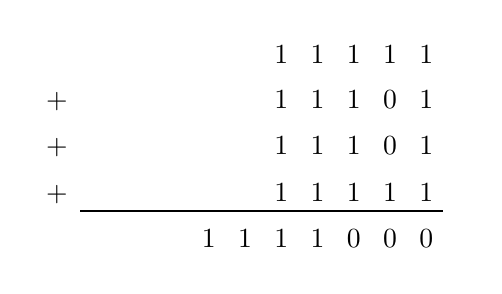
\begin{tikzpicture}[
    every node/.style={column sep=.5mm,row sep=1mm}]
    \matrix (m) [matrix of math nodes,
        nodes in empty cells,
        %nodes=draw
    ] 
    {
        &  &  &  &  &  &  &  & 1 & 1 & 1 & 1 & 1 &     \\
    +   &  &  &  &  &  &  &  & 1 & 1 & 1 & 0 & 1 &            \\
    +   &  &  &  &  &  &  &  & 1 & 1 & 1 & 0 & 1 &            \\
    +   &  &  &  &  &  &  &  & 1 & 1 & 1 & 1 & 1 &            \\
        &  &  &  &  &  & 1 & 1 & 1 & 1 & 0 & 0 &  0&            \\                                                  
    };

    \draw[-,color=black,semithick] (m-4-2.south west) -- (m-4-13.south east);

\end{tikzpicture}
\end{equation*}

The following example demonstrates the entire process by using different colors to distinguish each column and the corresponding carries they produce. Note that the last two digits in the sum are colored black, as they do not result from any specific column but are instead generated solely from the carries.

\begin{equation*}
\begin{tikzpicture}[
    row 1/.style={font=\textsl,font=\tiny, anchor=mid,
        inner sep=1.5pt},
    row 2/.style={font=\textsl,font=\tiny, anchor=mid,
        inner sep=1.5pt},
    row 3/.style={font=\textsl,font=\tiny, anchor=mid,
        inner sep=1.5pt},
    every node/.style={column sep=.5mm,row sep=1mm}]
    \matrix (m) [matrix of math nodes,
        nodes in empty cells,
        %nodes=draw
    ] 
    {
        &   &   &   &   &   &  \textcolor{YellowOrange}{1} &  \textcolor{YellowOrange}{0} &  &  &  &  &   &            \\
        &   &   &   &   &   &  & \textcolor{Purple}{1} & \textcolor{Purple}{0} &  & \textcolor{red}{1}  &  &   &            \\
        &   &   &   &   &   &  &  & \textcolor{Green}{1}  & \textcolor{Green}{1}  & \textcolor{blue}{1}  & \textcolor{blue}{0}  &   &            \\
        &  &  &  &  &  &  &  & \textcolor{YellowOrange}{1} & \textcolor{Purple}{1} & \textcolor{Green}{1}  & \textcolor{red}{1}  & \textcolor{blue}{1} &     \\
    +   &  &  &  &  &  &  &  &  \textcolor{YellowOrange}{1} & \textcolor{Purple}{1} & \textcolor{Green}{1}  & \textcolor{red}{0} & \textcolor{blue}{1}  &            \\
    +   &  &  &  &  &  &  &  &  \textcolor{YellowOrange}{1} & \textcolor{Purple}{1} & \textcolor{Green}{1}  & \textcolor{red}{0}  & \textcolor{blue}{1}  &            \\
    +   &  &  &  &  &  &  &  &  \textcolor{YellowOrange}{1} & \textcolor{Purple}{1} & \textcolor{Green}{1}  & \textcolor{red}{1}  & \textcolor{blue}{1}  &            \\
        &  &  &  &  &  & 1 & 1 &  \textcolor{YellowOrange}{1} & \textcolor{Purple}{1} & \textcolor{Green}{0}  & \textcolor{red}{0}  & \textcolor{blue}{1}  &            \\                                                  
    };

    \draw[-,color=black,semithick] (m-7-2.south west) -- (m-7-13.south east);

\end{tikzpicture}
\end{equation*}

\subsubsection*{Method 2: Direct Summation and Simplification}
We will illustrate the second method using the same example. In the previous case, we carried the actual binary number to the next columns. In this method, we write down 0 if the sum is even and 1 if the sum is odd. Every time a sum a multiple of 2, we carry a 1 to the next columns, and then continue this process for each column, including the carries in the calculation of that column.

\textbf{Step 1: Add the Rightmost Column}\newline
Add bits in column 1 (from counting from MSB):

$$
1+1+1+1=100_2 \quad(\text { which is binary for } 4)
$$
Reading the result from LSB to MSB
\begin{itemize}
    \item write down the 0
    \item carry a 1 for the first multiple of 2
    \item carry a 1 for the second multiple of 2
\end{itemize}
This results in


\begin{equation*}
\begin{tikzpicture}[
    row 1/.style={font=\textsl,font=\tiny, anchor=mid,
        inner sep=1.5pt},
    row 2/.style={font=\textsl,font=\tiny, anchor=mid,
        inner sep=1.5pt},
    row 3/.style={font=\textsl,font=\tiny, anchor=mid,
        inner sep=1.5pt},
    every node/.style={column sep=.5mm,row sep=1mm}]
    \matrix (m) [matrix of math nodes,
        nodes in empty cells,
        %nodes=draw
    ] 
    {
        &   &   &   &   &   &  &  &  &  &  &  &   &            \\
        &   &   &   &   &   &  &  &  &  &  & 1 &   &            \\
        &   &   &   &   &   &  &  & &  &  & 1 &   &            \\
        &  &  &  &  &  &  &  & 1 & 1 & 1 & 1 & 1 &     \\
    +   &  &  &  &  &  &  &  & 1 & 1 & 1 & 0 & 1 &            \\
    +   &  &  &  &  &  &  &  & 1 & 1 & 1 & 0 & 1 &            \\
    +   &  &  &  &  &  &  &  & 1 & 1 & 1 & 1 & 1 &            \\
        &  &  &  &  &  &  &  &  &  &  &  & 0 &            \\                                                  
    };

    \draw[-,color=black,semithick] (m-7-2.south west) -- (m-7-13.south east);

\end{tikzpicture}
\end{equation*}

\textbf{Step 2: Add the Second Column from the Right}\newline
Add bits in column 2 (from counting from MSB):

$$
1+1+1+1=100_2 \quad(\text { which is binary for } 4)
$$
Reading the result from LSB to MSB
\begin{itemize}
    \item write down the 0
    \item carry a 1 for the first multiple of 2
    \item carry a 1 for the second multiple of 2
\end{itemize}
This results in


\begin{equation*}
\begin{tikzpicture}[
    row 1/.style={font=\textsl,font=\tiny, anchor=mid,
        inner sep=1.5pt},
    row 2/.style={font=\textsl,font=\tiny, anchor=mid,
        inner sep=1.5pt},
    row 3/.style={font=\textsl,font=\tiny, anchor=mid,
        inner sep=1.5pt},
    every node/.style={column sep=.5mm,row sep=1mm}]
    \matrix (m) [matrix of math nodes,
        nodes in empty cells,
        %nodes=draw
    ] 
    {
        &   &   &   &   &   &  &  &  &  &  &  &   &            \\
        &   &   &   &   &   &  &  &  &  & 1  &  &   &            \\
        &   &   &   &   &   &  &  & &  & 1 &  &   &            \\
        &  &  &  &  &  &  &  & 1 & 1 & 1 & 1 & 1 &     \\
    +   &  &  &  &  &  &  &  & 1 & 1 & 1 & 0 & 1 &            \\
    +   &  &  &  &  &  &  &  & 1 & 1 & 1 & 0 & 1 &            \\
    +   &  &  &  &  &  &  &  & 1 & 1 & 1 & 1 & 1 &            \\
        &  &  &  &  &  &  &  &  &  &  & 0 & 0 &            \\                                                  
    };

    \draw[-,color=black,semithick] (m-7-2.south west) -- (m-7-13.south east);

\end{tikzpicture}
\end{equation*}

\textbf{Step 3: Add the Third Column from the Right}
Add bits in column 3 (from counting from MSB):

$$
1+1+1+1+1+1=110_2 \quad(\text { which is binary for } 6)
$$
Reading the result from LSB to MSB
\begin{itemize}
    \item write down the 0
    \item carry a 1 for the first multiple of 2
    \item carry a 1 for the second multiple of 2
    \item carry a 1 for the third multiple of 2
\end{itemize}

This results in


\begin{equation*}
\begin{tikzpicture}[
    row 1/.style={font=\textsl,font=\tiny, anchor=mid,
        inner sep=1.5pt},
    row 2/.style={font=\textsl,font=\tiny, anchor=mid,
        inner sep=1.5pt},
    row 3/.style={font=\textsl,font=\tiny, anchor=mid,
        inner sep=1.5pt},
    every node/.style={column sep=.5mm,row sep=1mm}]
    \matrix (m) [matrix of math nodes,
        nodes in empty cells,
        %nodes=draw
    ] 
    {
        &   &   &   &   &   &  &  &  & 1 &  &  &   &            \\
        &   &   &   &   &   &  &  &  & 1 &   &  &   &            \\
        &   &   &   &   &   &  &  & & 1 &  &  &   &            \\
        &  &  &  &  &  &  &  & 1 & 1 & 1 & 1 & 1 &     \\
    +   &  &  &  &  &  &  &  & 1 & 1 & 1 & 0 & 1 &            \\
    +   &  &  &  &  &  &  &  & 1 & 1 & 1 & 0 & 1 &            \\
    +   &  &  &  &  &  &  &  & 1 & 1 & 1 & 1 & 1 &            \\
        &  &  &  &  &  &  &  &  &  & 0 & 0 & 0 &            \\                                                  
    };

    \draw[-,color=black,semithick] (m-7-2.south west) -- (m-7-13.south east);

\end{tikzpicture}
\end{equation*}

\textbf{Step 4: Add the Fourth Column from the Right}\newline
Add bits in column 4 (from counting from MSB):

$$
1+1+1+1+1+1+1=111_2 \quad(\text { which is binary for } 7)
$$
Reading the result from LSB to MSB
\begin{itemize}
    \item write down the 1
    \item carry a 1 for the first multiple of 2
    \item carry a 1 for the second multiple of 2
    \item carry a 1 for the third multiple of 2
\end{itemize}
This results in


\begin{equation*}
\begin{tikzpicture}[
    row 1/.style={font=\textsl,font=\tiny, anchor=mid,
        inner sep=1.5pt},
    row 2/.style={font=\textsl,font=\tiny, anchor=mid,
        inner sep=1.5pt},
    row 3/.style={font=\textsl,font=\tiny, anchor=mid,
        inner sep=1.5pt},
    every node/.style={column sep=.5mm,row sep=1mm}]
    \matrix (m) [matrix of math nodes,
        nodes in empty cells,
        %nodes=draw
    ] 
    {
        &   &   &   &   &   &  &  & 1 &  &  &  &   &            \\
        &   &   &   &   &   &  &  & 1 &  &   &  &   &            \\
        &   &   &   &   &   &  &  & 1 &  &  &  &   &            \\
        &  &  &  &  &  &  &  & 1 & 1 & 1 & 1 & 1 &     \\
    +   &  &  &  &  &  &  &  & 1 & 1 & 1 & 0 & 1 &            \\
    +   &  &  &  &  &  &  &  & 1 & 1 & 1 & 0 & 1 &            \\
    +   &  &  &  &  &  &  &  & 1 & 1 & 1 & 1 & 1 &            \\
        &  &  &  &  &  &  &  &  & 1 & 0 & 0 & 0 &            \\                                                  
    };

    \draw[-,color=black,semithick] (m-7-2.south west) -- (m-7-13.south east);

\end{tikzpicture}
\end{equation*}


\textbf{Step 5: Add the Leftmost Column}\newline
Add bits in leftmost column):

$$
1+1+1+1+1+1+1=111_2 \quad(\text { which is binary for } 7)
$$
Reading the result from LSB to MSB
\begin{itemize}
    \item write down the result in binary, i.e. 1 1 1
\end{itemize}
This results in


\begin{equation*}
\begin{tikzpicture}[
    row 1/.style={font=\textsl,font=\tiny, anchor=mid,
        inner sep=1.5pt},
    row 2/.style={font=\textsl,font=\tiny, anchor=mid,
        inner sep=1.5pt},
    row 3/.style={font=\textsl,font=\tiny, anchor=mid,
        inner sep=1.5pt},
    every node/.style={column sep=.5mm,row sep=1mm}]
    \matrix (m) [matrix of math nodes,
        nodes in empty cells,
        %nodes=draw
    ] 
    {
        &   &   &   &   &   &  &  &  &  &  &  &   &            \\
        &   &   &   &   &   &  &  &  &  &   &  &   &            \\
        &   &   &   &   &   &  &  & &  &  &  &   &            \\
        &  &  &  &  &  &  &  & 1 & 1 & 1 & 1 & 1 &     \\
    +   &  &  &  &  &  &  &  & 1 & 1 & 1 & 0 & 1 &            \\
    +   &  &  &  &  &  &  &  & 1 & 1 & 1 & 0 & 1 &            \\
    +   &  &  &  &  &  &  &  & 1 & 1 & 1 & 1 & 1 &            \\
        &  &  &  &  &  & 1 & 1 & 1 & 1 & 0 & 0 & 0 &            \\                                                  
    };

    \draw[-,color=black,semithick] (m-7-2.south west) -- (m-7-13.south east);
\end{tikzpicture}
\end{equation*}

which corresponds to the result we obtained above. While not demonstrated explicitly here, subtraction works in a similar fashion.

By using one of these methods for handling multiple carries, allow us to also multiply two binary numbers.



\subsection*{Multiplication in Binary}
Multiplication in binary is technically easier than multiplication in decimal. In binary operations, we work exclusively with two digits: 0 and 1. This means that both the the multiplier\footnote{The "multiplicand" is the number that has to be multiplied, and the "multiplier" is the number by which it is multiplied.} and multiplicand consist of 0's and 1' (and so does the multiplicand). The process of finding the binary product is analogous to traditional multiplication in the decimal system. The four five steps involved in multiplying binary digits are:

\[
\begin{aligned}
& 0 \times 0=0 \\
& 0 \times 1=0 \\
& 1 \times 0=0 \\
& 1 \times 1=1 \\
& 1 \times 10_2 = 10_2 \quad \left( \text{multiplying by base } 10_2 \text{ adds a 0 to the end} \right)
\end{aligned}
\]

The last step means that $101_2 \times 10_2 = 1010_2$ which is analogous to the decimal case: $143_{10} \times 10_{10} = 1430_{10}$.

We will illustrate the process by supplying a couple of examples.

\begin{example}


\begin{equation*}
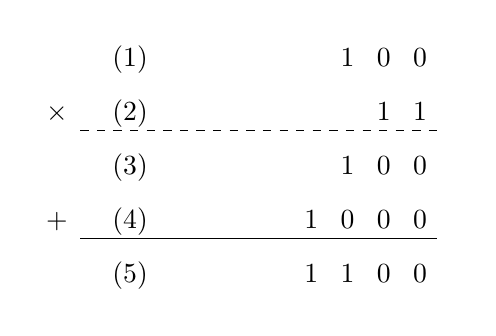
\begin{tikzpicture}[
    every node/.style={column sep=.5mm,row sep=1mm}]
    \matrix (m) [matrix of math nodes,
        nodes in empty cells,
        %nodes=draw
    ] 
    {
        &   &  (1) &   &   &   &  &  &  &  & 1 & 0 & 0  &            \\
     \times   &   & (2)  &   &   &   &  &  &  &  &   & 1 &  1 &            \\
        &   & (3)  &   &   &   &  &  & &  & 1 & 0 & 0  &            \\
       + &  & (4) &  &  &  &  &  &  & 1 & 0 & 0 & 0 &     \\
        &  & (5) &  &  &  &  &  &  & 1 & 1 & 0 & 0 &            \\                                                  
    };

    \draw[dashed, color=black, semithick] (m-2-2.south west) -- (m-2-13.south east);
    \draw[-,color=black,semithick] (m-4-2.south west) -- (m-4-13.south east);
    \end{tikzpicture}
\end{equation*}

Here are the steps:

\begin{itemize}
    \item Multiply the multiplicand (line 1) by the LSB of the multiplier (line 2), which in this case is 1.
    \item Record this result in line 3.
    \item Append a 0 to line 4 to account for the shift to the next power of 2 in the multiplier.
    \item Multiply the multiplicand (line 1) by the next bit of the multiplier (line 2), which is also 1 in this case.
    \item Add this result to line 4, after the 0 you appended earlier.
    \item Finally, sum the values in lines 3 and 4, as outlined in the previous section, to obtain the final result in line 5.
\end{itemize}
\end{example}

We offer two additional examples:

\begin{example}

\begin{equation*}
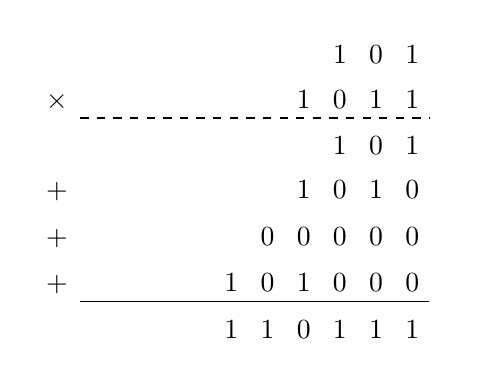
\begin{tikzpicture}[
    every node/.style={column sep=.5mm,row sep=1mm}]
    \matrix (m) [matrix of math nodes,
        nodes in empty cells,
        %nodes=draw
    ] 
    {
        &   &   &   &   &   &  &  &  &  & 1 & 0 & 1  &            \\
     \times   &   &   &   &   &   &  &  &  & 1 &  0 & 1 &  1 &            \\
        &   &   &   &   &   &  &  & &  & 1 & 0 & 1  &            \\
       + &  &  &  &  &  &  &  &  & 1 & 0 & 1 & 0 &     \\
       + &  &  &  &  &  &  &  & 0 & 0 & 0 & 0 & 0 &            \\               
       + &  &  &  &  &  &  & 1 & 0 & 1 & 0 & 0 & 0 &     \\
        &  &  &  &  &  &  & 1 & 1 & 0 & 1 & 1 & 1 &            \\                                        
    };

    \draw[dashed, color=black, semithick] (m-2-2.south west) -- (m-2-13.south east);
    \draw[-,color=black,semithick] (m-6-2.south west) -- (m-6-13.south east);
    \end{tikzpicture}
\end{equation*}
    
\end{example}

\begin{example}
\label{ex1.3}
\begin{equation*}
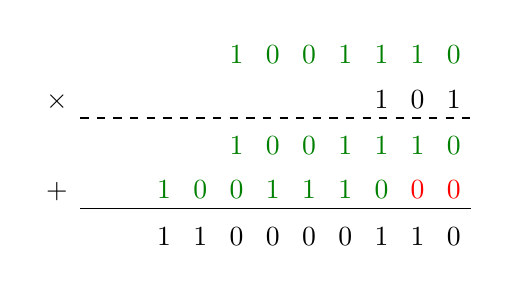
\begin{tikzpicture}[
    every node/.style={column sep=.5mm,row sep=1mm}]
    \matrix (m) [matrix of math nodes,
        nodes in empty cells,
        %nodes=draw
    ] 
    {
        &   &   &   &   &   & \textcolor{Green}{1} & \textcolor{Green}{0} & \textcolor{Green}{0} & \textcolor{Green}{1} & \textcolor{Green}{1} & \textcolor{Green}{1} & \textcolor{Green}{0}  &            \\
     \times   &   &   &   &   &   &  &  &  &  &  1 & 0 &  1 &            \\
        &   &   &   &   &   & \textcolor{Green}{1} & \textcolor{Green}{0} & \textcolor{Green}{0} & \textcolor{Green}{1} & \textcolor{Green}{1} & \textcolor{Green}{1} & \textcolor{Green}{0}   &            \\
       + &  &  &  & \textcolor{Green}{1} & \textcolor{Green}{0} & \textcolor{Green}{0} & \textcolor{Green}{1} & \textcolor{Green}{1} & \textcolor{Green}{1} & \textcolor{Green}{0} & \textcolor{Red}{0} & \textcolor{Red}{0} &            \\             
        &  &  &  & 1 & 1 & 0 & 0 & 0 & 0 & 1 & 1 & 0 &     \\                                     
    };

    \draw[dashed, color=black, semithick] (m-2-2.south west) -- (m-2-13.south east);
    \draw[-,color=black,semithick] (m-4-2.south west) -- (m-4-13.south east);
    \end{tikzpicture}
\end{equation*}
    
\end{example}

In \autoref{ex1.3} notice that we omitted the row of zeroes that the second value of the multiplier would have produced, and notice even further that we added two 0's before restating the multiplicand in the sum.

Binary multiplication, like binary addition, is a core operation in computer arithmetic. By breaking the process down into manageable steps—multiplying individual bits and then summing the results—it becomes clear how similar it is to the multiplication methods we use in the decimal system. The main difference is the simplicity and efficiency of working within the binary system, where only the digits 0 and 1 are involved.

We notice how binary multiplication builds on binary addition. Each step, involving shifts and sums, essentially consists of repeated additions adjusted by powers of two. A strong grasp of binary addition naturally leads to a better understanding of binary multiplication and its applications.

\section{Octal and Hexadecimal}
Octal is a base-8 numbering system that uses the digits 0 through 7. It is closely related to binary, which is a base-2 system. The connection between the two lies in how easily binary numbers can be converted to octal and vice versa. Each octal digit corresponds to exactly three binary digits (bits), making conversions straightforward. For example, the binary number `110` converts directly to the octal digit `6`. Because of this close relationship, octal is often used as a shorthand for binary in computing, particularly in contexts where grouping binary digits in sets of three simplifies reading and interpreting binary data.

\[
\begin{aligned}
12_8 &= 1 \cdot 8^1 + 2 \cdot 8^0  = 10_{10} \\
3021_8 & = 3 \cdot 8^3 + 0 \cdot 8^2 + 2 \cdot 8^1 + 1 \cdot 8^0 = 1553_{10}
\end{aligned}
\]

Since \(8\) is \(2^3\), we can express it in binary:

\[
\begin{aligned}
3 & \rightarrow \textcolor{Green}{011} \\
0 & \rightarrow \textcolor{YellowOrange}{000} \\
2 & \rightarrow \textcolor{blue}{010} \\
1 & \rightarrow \textcolor{red}{001} \\
\end{aligned}
\]

\[
\text{Thus, } 3021_8 = \textcolor{Green}{011}\textcolor{YellowOrange}{000} \textcolor{blue}{010}\textcolor{red}{001}_2 = \textcolor{Green}{11}\textcolor{YellowOrange}{000} \textcolor{blue}{010}\textcolor{red}{001}_2
\]

We obtain the final result by removing leading zeros.

Hexadecimal is a base-16 numbering system that uses sixteen distinct symbols: the digits 0-9 and the letters A-F, where A represents 10, B represents 11, and so on up to F, which represents 15. Hexadecimal is closely related to binary because each hexadecimal digit corresponds exactly to four binary digits (bits). This direct relationship makes it easy to convert between the two systems. For example, the hexadecimal digit `A` translates to the binary sequence `1010`. Due to this efficiency in grouping, hexadecimal is often used in computing as a more compact and readable way to represent binary data, particularly in areas like memory addresses and colour codes in web design.

\[
\begin{aligned}
123_{16} &= 1 \cdot 16^2 + 2 \cdot 16^1 + 3 \cdot 16^0  = 256 + 32 + 3 = 291_{10} \\
A2E_{16} & = 10 \cdot 16^2 + 2 \cdot 16^1 + 14 \cdot 16^0 = 2560 + 32 + 14 = 2606_{10}
\end{aligned}
\]

Since \(16\) is \(2^4\), we can, for instance, express $A2E_{16}$ in binary:

\[
\begin{aligned}
A & \rightarrow 1010 \\
2 & \rightarrow 0010 \\
E & \rightarrow 1110 \\
\end{aligned}
\]

\[
\text{Thus, } A2E_{16} = 101000101110_2
\]

Similarly we get $5EB52_{16}$ as

\[
\begin{aligned}
5 & \rightarrow 0101 \\
E & \rightarrow 1110 \\
B & \rightarrow 1011 \\
5 & \rightarrow 0101 \\
2 & \rightarrow 0010 \\
\end{aligned}
\]

\[
\text{Thus, } 5EB52_{16} = 01011110101101010010_2
\]

Again, notice that we removed the leading 0's from $5_{16}$ when writing the result.

\section{Converting Between Systems}

Understanding how to convert numbers between binary, decimal, octal, and hexadecimal systems is essential in computer science and digital electronics. Each system is a different base, and each has its own applications. Here's a step-by-step guide to help you convert numbers from one system to another.

\subsection*{Decimal to Binary Conversion}
To convert a decimal number to binary:
\begin{enumerate}
    \item Divide the decimal number by 2.
    \item Record the remainder (it will be 0 or 1).
    \item Divide the quotient by 2 and record the remainder.
    \item Repeat until the quotient is 0.
    \item The binary number is the sequence of remainders read from bottom to top.
\end{enumerate}

\begin{example} Convert \(23_{10}\) to binary.

\begin{solution}

\[
\begin{aligned}
23 \div 2 & = 11 \quad \text{remainder } 1 \\
11 \div 2 & = 5 \quad \text{remainder } 1 \\
5 \div 2 & = 2 \quad \text{remainder } 1 \\
2 \div 2 & = 1 \quad \text{remainder } 0 \\
1 \div 2 & = 0 \quad \text{remainder } 1 \\
\end{aligned}
\]
Thus, \(23_{10} = 10111_2\). \end{solution}
\end{example}

\subsection*{Decimal to Octal Conversion}
To convert a decimal number to octal:
\begin{enumerate}
    \item Divide the decimal number by 8.
    \item Record the remainder.
    \item Divide the quotient by 8 and record the remainder.
    \item Repeat until the quotient is 0.
    \item The octal number is the sequence of remainders read from bottom to top.
\end{enumerate}

\begin{example}Convert \(78_{10}\) to octal.

\begin{solution}
    


\[
\begin{aligned}
78 \div 8 & = 9 \quad \text{remainder } 6 \\
9 \div 8 & = 1 \quad \text{remainder } 1 \\
1 \div 8 & = 0 \quad \text{remainder } 1 \\
\end{aligned}
\]
Thus, \(78_{10} = 116_8\). \end{solution}
    
\end{example}

\subsection*{Decimal to Hexadecimal Conversion}
To convert a decimal number to hexadecimal:
\begin{enumerate}
    \item Divide the decimal number by 16.
    \item Record the remainder (use A, B, C, D, E, F for remainders 10, 11, 12, 13, 14, 15 respectively).
    \item Divide the quotient by 16 and record the remainder.
    \item Repeat until the quotient is 0.
    \item The hexadecimal number is the sequence of remainders read from bottom to top.
\end{enumerate}

\begin{example}Convert \(255_{10}\) to hexadecimal.

\begin{solution}
    
\[
\begin{aligned}
255 \div 16 & = 15 \quad \text{remainder } 15 \quad (\text{F}) \\
15 \div 16 & = 0 \quad \text{remainder } 15 \quad (\text{F}) \\
\end{aligned}
\]
Thus, \(255_{10} = FF_{16}\).\end{solution}

\end{example}


\subsection*{Binary to Decimal Conversion}
To convert a binary number to decimal:
\begin{enumerate}
    \item Multiply each bit by 2 raised to the power of its position, starting from 0 on the right.
    \item Sum all the products.
\end{enumerate}

Notice that this amounts to the method outlined above about binary expansion.

\begin{example} Convert \(1101_2\) to decimal.

\begin{solution}
    

\[
\begin{aligned}
1 \cdot 2^3 + 1 \cdot 2^2 + 0 \cdot 2^1 + 1 \cdot 2^0 & = 8 + 4 + 0 + 1 = 13_{10}
\end{aligned}
\] \end{solution}

\end{example}

\subsection*{Binary to Octal Conversion}
To convert a binary number to octal:
\begin{enumerate}
    \item Group the binary digits into sets of three, starting from the right. Add leading zeros if necessary.
    \item Convert each group of three binary digits to its octal equivalent.
\end{enumerate}

\begin{example}Convert \(110110_2\) to octal.

\begin{solution}
\[
\begin{aligned}
110 & \rightarrow 6 \\
110 & \rightarrow 6 \\
\end{aligned}
\]
Thus, \(110110_2 = 66_8\). \end{solution}

\end{example}

\subsection*{Binary to Hexadecimal Conversion}
To convert a binary number to hexadecimal:
\begin{enumerate}
    \item Group the binary digits into sets of four, starting from the right. Add leading zeros if necessary.
    \item Convert each group of four binary digits to its hexadecimal equivalent.
\end{enumerate}

\begin{example}Convert \(10110101_2\) to hexadecimal.

\begin{solution}
\[
\begin{aligned}
1011 & \rightarrow B \\
0101 & \rightarrow 5 \\
\end{aligned}
\]
Thus, \(10110101_2 = B5_{16}\). \end{solution}

\end{example}

\subsection*{Octal to Binary Conversion}
To convert an octal number to binary: Convert each octal digit to its 3-bit binary equivalent!

\begin{example}Convert \(57_8\) to binary.

\begin{solution}
\[
\begin{aligned}
5 & \rightarrow 101 \\
7 & \rightarrow 111 \\
\end{aligned}
\]
Thus, \(57_8 = 101111_2\). \end{solution}

\end{example}

\subsection*{Octal to Decimal Conversion}
To convert an octal number to decimal:
\begin{enumerate}
    \item Multiply each digit by 8 raised to the power of its position, starting from 0 on the right.
    \item Sum all the products.
\end{enumerate}

\begin{example}Convert \(157_8\) to decimal.

\begin{solution}
    
\[
\begin{aligned}
1 \cdot 8^2 + 5 \cdot 8^1 + 7 \cdot 8^0 & = 64 + 40 + 7 = 111_{10}
\end{aligned}
\] \end{solution}

\end{example}

\subsection*{Octal to Hexadecimal Conversion}
To convert an octal number to hexadecimal:
\begin{enumerate}
    \item First, convert the octal number to binary.
    \item Then, convert the binary number to hexadecimal by grouping the binary digits in sets of four.
\end{enumerate}

\begin{example}Convert \(157_8\) to hexadecimal.

\begin{solution}

\[
\begin{aligned}
1 & \rightarrow 001 \\
5 & \rightarrow 101 \\
7 & \rightarrow 111 \\
\end{aligned}
\]
Thus, \(157_8 = 001101111_2 = 6F_{16}\). \end{solution}
\end{example}

\subsection*{Hexadecimal to Binary Conversion}
To convert a hexadecimal number to binary: Convert each hexadecimal digit to its 4-bit binary equivalent.

\begin{example}Convert \(2B_{16}\) to binary.

\begin{solution}
    


\[
\begin{aligned}
2 & \rightarrow 0010 \\
B & \rightarrow 1011 \\
\end{aligned}
\]
Thus, \(2B_{16} = 00101011_2\).\end{solution}

\end{example}

\subsection*{Hexadecimal to Decimal Conversion}
To convert a hexadecimal number to decimal:
\begin{enumerate}
    \item Multiply each digit by 16 raised to the power of its position, starting from 0 on the right.
    \item Sum all the products.
\end{enumerate}

\begin{example}Convert \(2B_{16}\) to decimal.

\begin{solution}
\[
\begin{aligned}
2 \cdot 16^1 + 11 \cdot 16^0 & = 32 + 11 = 43_{10}
\end{aligned}
\] \end{solution}
\end{example}

\subsection*{Hexadecimal to Octal Conversion}
To convert a hexadecimal number to octal:
\begin{enumerate}
    \item First, convert the hexadecimal number to binary.
    \item Then, convert the binary number to octal by grouping the binary digits in sets of three.
\end{enumerate}

\begin{example}Convert \(2B_{16}\) to octal.

\begin{solution}

\[
\begin{aligned}
2 & \rightarrow 0010 \\
B & \rightarrow 1011 \\
\end{aligned}
\]
Thus, \(2B_{16} = 00101011_2 = 53_8\). \end{solution}

\end{example}

\subsection*{Final Thoughts on Conversion}
The concept of expansion plays a central role in these conversions. Whether you are expanding a decimal number into its binary, octal, or hexadecimal form, or converting a binary number into its octal or hexadecimal equivalent, you are more or less expressing the number in terms of powers of the base. The expansion method is essentially the same for each system as it boils down to dividing by the highest power of the base recursively:

$$
\begin{aligned}
7562_{10} & =1 \cdot 16^3+3466=1 \cdot 16^3+13 \cdot 16^2+138 \\
& =\textcolor{red}{1} \cdot 16^3+ \textcolor{blue}{13} \cdot 16^2+\textcolor{YellowOrange}{8} \cdot 16^1+\textcolor{Green}{10} \cdot 16^0=\textcolor{red}{1} \, \textcolor{blue}{D} \, \textcolor{YellowOrange}{8} \, \textcolor{Green}{A}
\end{aligned}
$$

By understanding these expansions and the relationships between these number systems, you can efficiently switch between them, allowing you to represent and manipulate data in the most suitable format for any given situation.

\chapter{Numeral Systems}
\label{chap:ch3}

We are so accustomed to working within the decimal system that we often forget it is a relatively recent invention and was once considered revolutionary. It is time to carefully examine how we represent numbers. Typically, we use the decimal system, where a number like 3459 is shorthand for \(3 \times 1000 + 4 \times 100 + 5 \times 10 + 9\). The position of each digit is crucial, as it allows us to distinguish between values like 30 and 3. The decimal system is a\textbf{ positional numeral system}, meaning it has designated positions for units, tens, hundreds, and so forth. Each digit’s position implies the multiplier (a power of ten) that should be used with that digit, and each position has a value ten times that of the position to its right.

Notice that we can save space by writing 1000 as \(10^3\), where the exponent 3 indicates the number of zeros. Thus, \(100000 = 10^5\). If the exponent is negative, it represents a fraction, e.g., \(10^{-3} = \frac{1}{1000}\). Perhaps the most ingenious aspect of the positional system was the addition of the decimal point, which allows us to include decimal fractions. For example, the number 123.456 is equivalent to:
\[
1 \times 100 + 2 \times 10 + 3 \times 1 + 4 \times \frac{1}{10} + 5 \times \frac{1}{100} + 6 \times \frac{1}{1000}.
\]

This can be visualised as:
\[
\begin{array}{rccccccccc}
\text{Multiplier:} & \ldots & 10^2 & 10^1 & 10^0 & . & 10^{-1} & 10^{-2} & 10^{-3} & \ldots \\
\text{Digits:} & \ldots & 1 & 2 & 3 & . & 4 & 5 & 6 &\ldots \\
& & & & & \uparrow & & & & \\
& & & & & \text{Decimal Point:} & & & &
\end{array}
\]
However, there is no inherent reason why we must use powers of 10, or base 10. The Babylonians, for instance, used base 60, and base 12 was very common in medieval Europe. Today, the most widely used numeral systems are summarised in \autoref{tab:number_systems}

\begin{table}[ht]
\centering
\renewcommand{\arraystretch}{1.4}
\begin{tabular}{|c|c|c|c|}
\hline
\textbf{Numeral system} & \textbf{Symbols} & \textbf{Base} & \textbf{Additional information} \\ \hline
\textbf{Decimal} & 0-9 & 10 & - \\ \hline
\textbf{Binary} & 0, 1 & 2 & - \\ \hline
\textbf{Hexadecimal} & 0-9, A-F & 16 & $\mathrm{A} \equiv 10, \mathrm{B} \equiv 11, \mathrm{C} \equiv 12,$ $\mathrm{D} \equiv 13, \mathrm{E} \equiv 14, \mathrm{F} \equiv 15$ \\ \hline
\textbf{Octal} & 0-7 & 8 & - \\ \hline
\end{tabular}
\caption{Summary of Common Numeral Systems}
\label{tab:number_systems}
\end{table}

We begin by focusing on binary which will also receive the most detailed attention in this chapter.

\section{Binary Numbers}
In the binary scale, we express numbers in powers of 2 rather than the 10s of the decimal scale. For some numbers, this is easy. Recall $2^0=1$,

\begin{table}[!ht]
\centering
\renewcommand{\arraystretch}{1.4}
\begin{tabular}{|c c c c c c c c|}
\hline 
\multirow{2}{*}{Decimal number} & & \multirow{2}{*}{In powers of 2} & \multicolumn{4}{c}{Power of 2} & \multirow{2}{*}{Binary number} \\
& & & 3 & 2 & 1 & 0 & \\ \hline
8 & $=$ & $2^3$ & 1 & 0 & 0 & 0 & 1000 \\
7 & $=$ & $2^2 + 2^1 + 2^0$ & 0 & 1 & 1 & 1 & 111 \\
6 & $=$ & $2^2 + 2^1$ & 0 & 1 & 1 & 0 & 110 \\
5 & $=$ & $2^2 + 2^0$ & 0 & 1 & 0 & 1 & 101 \\
4 & $=$ & $2^2$ & 0 & 1 & 0 & 0 & 100 \\
3 & $=$ & $2^1 + 2^0$ & 0 & 0 & 1 & 1 & 11 \\
2 & $=$ & $2^1$ & 0 & 0 & 1 & 0 & 10 \\
1 & $=$ & $2^0$ & 0 & 0 & 0 & 1 & 1 \\ \hline
\end{tabular}
\caption{Decimal Numbers in Binary Representation}
\end{table}

As in decimal, we write this with the position of the digit representing the power, the first place after the decimal being the $2^0$ position, the next the $2^1$, and so on. To convert a decimal number to binary, we can use the \texttt{mod} operator.

As an example, consider 88 in decimal or $88_{10}$. We would like to write it as a binary number. We take the number and successively divide \texttt{mod} 2. See below:

\begin{table}[h!]
\centering
\renewcommand{\arraystretch}{1.4}
\begin{tabular}{|c|c|c|c|c|}
\hline 
Step Number $n$ & $x_n$ & $x_n / 2$ & $x_n \bmod 2$ \\ \hline
0 & 88 & 44 & 0 \\ 
1 & 44 & 22 & 0 \\
2 & 22 & 11 & 0 \\
3 & 11 & 5 & 1 \\
4 & 5 & 2 & 1 \\
5 & 2 & 1 & 0 \\
6 & 1 & 0 & 1 \\ \hline
\end{tabular}
\caption{Conversion of Decimal 88 to Binary}
\end{table}

Writing the last column in reverse, that is from the bottom up, we have 1011000, which is the binary form of 88, i.e., $88_{10} = 1011000_2$.

Binary decimals are less common but quite possible. Thus, 101.1011 is just $2^2 + 2^0 + 2^{-1} + 2^{-3} + 2^{-4}$, which is, after some calculation, 5.6875. We have seen how to turn the integer part of a decimal number into a binary number, and we can do the same with a decimal fraction. Consider 0.6875. As before, we draw up a table:

\begin{table}[h!]
\centering
\renewcommand{\arraystretch}{1.4}
\begin{tabular}{|c|c|c|c|}
\hline 
Step Number $n$ & $x_n$ & $x_n \times 2$ & $\left\lfloor x_n \times 2 \right\rfloor$ \\ \hline
0 & 0.6875 & 1.375 & 1 \\ \hline
1 & 0.375 & 0.75 & 0 \\ \hline
2 & 0.75 & 1.5 & 1 \\ \hline
3 & 0.5 & 1 & 1 \\ \hline
\end{tabular}
\caption{Conversion of Decimal Fraction 0.6875 to Binary}
\end{table}

Giving, reading down, $0.6875_{10} = 1011_2$.

\subsection*{Binary Expansion}

The process outlined in the previous section is called \textbf{binary expansion} and refers to the representation of a number in the binary (base-2) numeral system. Every decimal number can be expressed as a sum of powers of 2, where each power corresponds to a binary digit (bit) in the number's binary form.

Let's reconsider the decimal number 88. To find its binary expansion, we identify the largest power of 2 less than or equal to 88 and continue subtracting powers of 2 until we reach 0.

First, we note that $2^6 = 64$ is the largest power of 2 less than 88:
\[
88 = 64 + 24
\]

Next, we find that $2^4 = 16$ is the largest power of 2 less than 24:
\[
24 = 16 + 8
\]

Finally, $2^3 = 8$ exactly matches the remainder:
\[
8 = 8 + 0
\]

Thus, we have:
\[
88 = 2^6 + 2^4 + 2^3
\]

In binary, each of these powers of 2 is represented by a '1' in the corresponding place value, with '0' in place values where no power of 2 contributes:
\[
88_{10} = 1011000_2
\]

To summarise:
\begin{itemize}
    \item $2^6 = 64$ corresponds to the leftmost '1' in the binary expansion.
    \item $2^4 = 16$ corresponds to the next '1'.
    \item $2^3 = 8$ corresponds to the next '1'.
    \item The remaining digits are '0' because $2^5$, $2^2$, $2^1$, and $2^0$ do not contribute to the value 88.
\end{itemize}

Thus, the binary expansion of 88 is $1011000_2$. This method of representing numbers is fundamental in computer science and digital electronics, where binary representation is the standard for data storage and processing.

\subsection*{Binary Operations}
Binary operations are basic arithmetic operations performed on binary numbers. These operations are essential in computing and digital systems, as they form the foundation for how computers process and manipulate data.

Binary addition, subtraction, and multiplication are similar to their decimal counterparts but follow simpler rules due to the binary system's limited digits. For example, binary addition follows these rules:

\[
0 + 0 = 0, \quad 0 + 1 = 1, \quad 1 + 0 = 1, \quad 1 + 1 = 10
\]

In this case, \(1 + 1\) results in \(10_2\), which means 0 with a carry of 1 to the next higher bit. Binary subtraction and multiplication follow similar straightforward rules that are easy to implement in digital systems.

The XOR (exclusive OR) operation is another important binary operation. XOR produces a 1 if the two bits being compared are different and a 0 if they are the same:

\[
0 \oplus 0 = 0, \quad 0 \oplus 1 = 1, \quad 1 \oplus 0 = 1, \quad 1 \oplus 1 = 0
\]

In binary addition, the XOR operation is used to add two bits without considering any carry from a previous bit. This is because XOR effectively performs addition modulo 2, which aligns perfectly with how binary addition works. For example:

\[
\begin{array}{c|c|c|c}
\text{Bit 1} & \text{Bit 2} & \text{XOR (Sum)} & \text{AND (Carry)} \\
\hline
0 & 0 & 0 & 0 \\
0 & 1 & 1 & 0 \\
1 & 0 & 1 & 0 \\
1 & 1 & 0 & 1 \\
\end{array}
\]

In the case of \(1 + 1\), XOR gives a sum of 0 and an AND operation (which detects the carry) gives a carry of 1, resulting in the binary number 10.

\begin{align*}
0 + 0 &= 0 \\
0 + 1 &= 1 \\
1 + 1 &= 10 \quad \text{so we carry 1 and leave a zero} \\
1 + 1 + 1 &= 1 + (1 + 1) = 1 + 10 = 11.
\end{align*}

We can write this in very much the same way as for a decimal addition:

\[
\begin{array}{r|r|r|r|r|r|r|r}
& 1 & 1 & 0 & 1 & 0 & 1 & \\
+ & 1 & 0 & 1 & 1 & 1 & 0 & \\
\hline
1 & 1 & 0 & 0 & 0 & 1 & 1 & \quad \text{Sum} \\
\uparrow & & & & \uparrow & & & \\
& & & & & & &
\end{array}
\]

The right-hand arrow shows where we carry a 1. The left-hand arrow shows where we have $1 + 1 + 1$ so we carry a 1 and have a 1 left over.

As we will see below, we will often need to handle multiple carries. There are two ways to handle this which resemble the methods we know from the decimal system. We will explain using an example.

\subsubsection*{Method 1: Column-wise Binary Addition with Multiple Carries}
Consider

\begin{equation*}
\begin{tikzpicture}[
    every node/.style={column sep=.5mm,row sep=1mm}]
    \matrix (m) [matrix of math nodes,
        nodes in empty cells,
        %nodes=draw
    ] 
    {
        &  &  &  &  &  &  &  & 1 & 1 & 1 & 1 & 1 &     \\
    +   &  &  &  &  &  &  &  & 1 & 1 & 1 & 0 & 1 &            \\
    +   &  &  &  &  &  &  &  & 1 & 1 & 1 & 0 & 1 &            \\
    +   &  &  &  &  &  &  &  & 1 & 1 & 1 & 1 & 1 &            \\
        &  &  &  &  &  &  &  &  &  &  &  &  &            \\                                                  
    };

    \draw[-,color=black,semithick] (m-4-2.south west) -- (m-4-13.south east);

\end{tikzpicture}
\end{equation*}

\textbf{Step 1: Add the Rightmost Column }\newline
Start by adding the rightmost bits:

$$
1+1+1+1=100_2 \quad(\text { which is binary for } 4)
$$
Reading the result from right to left (i.e. from \textit{least significant bit} (LSB) to the \textit{most significant bit}(MSB))
\begin{itemize}
    \item write down the 0
    \item carry the 0 to the next column
    \item carry the 1 to the third column
\end{itemize}
You end up with

\begin{equation*}
\begin{tikzpicture}[
    row 1/.style={font=\textsl,font=\tiny, anchor=mid,
        inner sep=1.5pt},
    every node/.style={column sep=.5mm,row sep=1mm}]
    \matrix (m) [matrix of math nodes,
        nodes in empty cells,
        %nodes=draw
    ] 
    {
        &   &   &   &   &   &  &  &  &  & 1 & 0 &   &            \\
        &  &  &  &  &  &  &  & 1 & 1 & 1 & 1 & 1 &     \\
    +   &  &  &  &  &  &  &  & 1 & 1 & 1 & 0 & 1 &            \\
    +   &  &  &  &  &  &  &  & 1 & 1 & 1 & 0 & 1 &            \\
    +   &  &  &  &  &  &  &  & 1 & 1 & 1 & 1 & 1 &            \\
        &  &  &  &  &  &  &  &  &  &  &  & 0 &            \\                                                  
    };

    \draw[-,color=black,semithick] (m-5-2.south west) -- (m-5-13.south east);

\end{tikzpicture}
\end{equation*}

\textbf{Step 2: Add the Second Column from the Right}\newline
Next, add the second column:



$$
0+1+0+0+1=10_2 \quad(\text { which is binary for } 2)
$$
Reading the result from LSB to MSB:
\begin{itemize}
    \item write down the 0
    \item carry the 1 to the next column
\end{itemize}
You end up with

\begin{equation*}
\begin{tikzpicture}[
    row 1/.style={font=\textsl,font=\tiny, anchor=mid,
        inner sep=1.5pt},
    row 2/.style={font=\textsl,font=\tiny, anchor=mid,
        inner sep=1.5pt},
    every node/.style={column sep=.5mm,row sep=1mm}]
    \matrix (m) [matrix of math nodes,
        nodes in empty cells,
        %nodes=draw
    ] 
    {
        &   &   &   &   &   &  &  &  &  & 1 &  &   &            \\
        &   &   &   &   &   &  &  &  &  & 1 &  &   &            \\
        &  &  &  &  &  &  &  & 1 & 1 & 1 & 1 & 1 &     \\
    +   &  &  &  &  &  &  &  & 1 & 1 & 1 & 0 & 1 &            \\
    +   &  &  &  &  &  &  &  & 1 & 1 & 1 & 0 & 1 &            \\
    +   &  &  &  &  &  &  &  & 1 & 1 & 1 & 1 & 1 &            \\
        &  &  &  &  &  &  &  &  &  &  & 0 & 0 &            \\                                                  
    };

    \draw[-,color=black,semithick] (m-6-2.south west) -- (m-6-13.south east);

\end{tikzpicture}
\end{equation*} \newpage


\textbf{Step 3: Add the Third Column from the Right}\newline
Now, add the third column:

$$
1+1+1+1+1+1=110_2 \quad(\text { which is binary for } 6)
$$
Reading the result from LSB to MSB
\begin{itemize}
    \item write down the 0
    \item carry the 1 to the fourth column
    \item carry the 1 to the fifth column
\end{itemize}
You end up with

Our sum so far:

\begin{equation*}
\begin{tikzpicture}[
    row 1/.style={font=\textsl,font=\tiny, anchor=mid,
        inner sep=1.5pt},
    every node/.style={column sep=.5mm,row sep=1mm}]
    \matrix (m) [matrix of math nodes,
        nodes in empty cells,
        %nodes=draw
    ] 
    {
        &   &   &   &   &   &  &  & 1 & 1 &  &  &   &            \\
        &  &  &  &  &  &  &  & 1 & 1 & 1 & 1 & 1 &     \\
    +   &  &  &  &  &  &  &  & 1 & 1 & 1 & 0 & 1 &            \\
    +   &  &  &  &  &  &  &  & 1 & 1 & 1 & 0 & 1 &            \\
    +   &  &  &  &  &  &  &  & 1 & 1 & 1 & 1 & 1 &            \\
        &  &  &  &  &  &  &  &  &  & 0 & 0 & 0 &            \\                                                  
    };

    \draw[-,color=black,semithick] (m-5-2.south west) -- (m-5-13.south east);

\end{tikzpicture}
\end{equation*}


\textbf{Step 4: Add the Fourth Column from the Right}\newline
Move to the fourth column:

$$
1+1+1+1+1=101_2 \quad(\text { which is binary for } 5)
$$

Reading the result from LSB to MSB
\begin{itemize}
    \item write down the 1
    \item carry the 0 to the fifth column
    \item carry the 1 to the sixth column
\end{itemize}
You end up with

\begin{equation*}
\begin{tikzpicture}[
    row 1/.style={font=\textsl,font=\tiny, anchor=mid,
        inner sep=1.5pt},
    row 2/.style={font=\textsl,font=\tiny, anchor=mid,
        inner sep=1.5pt},
    every node/.style={column sep=.5mm,row sep=1mm}]
    \matrix (m) [matrix of math nodes,
        nodes in empty cells,
        %nodes=draw
    ] 
    {
        &   &   &   &   &   &  &  & 0 &  &  &  &   &            \\
        &   &   &   &   &   &  & 1 & 1 &  &  &  &   &            \\
        &  &  &  &  &  &  &  & 1 & 1 & 1 & 1 & 1 &     \\
    +   &  &  &  &  &  &  &  & 1 & 1 & 1 & 0 & 1 &            \\
    +   &  &  &  &  &  &  &  & 1 & 1 & 1 & 0 & 1 &            \\
    +   &  &  &  &  &  &  &  & 1 & 1 & 1 & 1 & 1 &            \\
        &  &  &  &  &  &  &  &  & 1 & 0 & 0 & 0 &            \\                                                  
    };

    \draw[-,color=black,semithick] (m-6-2.south west) -- (m-6-13.south east);

\end{tikzpicture}
\end{equation*}

\textbf{Step 5: Add the Leftmost Column}\newline
Add the leftmost column:

$$
1+1+1+1+1=101_2 \quad(\text { which is binary for } 5)
$$
Reading the result from LSB to MSB
\begin{itemize}
    \item write down the 1
    \item carry the 0 to the sixth column
    \item carry the 1 to the seventh column
\end{itemize}
This results in

\begin{equation*}
\begin{tikzpicture}[
    row 1/.style={font=\textsl,font=\tiny, anchor=mid,
        inner sep=1.5pt},
    row 2/.style={font=\textsl,font=\tiny, anchor=mid,
        inner sep=1.5pt},
    every node/.style={column sep=.5mm,row sep=1mm}]
    \matrix (m) [matrix of math nodes,
        nodes in empty cells,
        %nodes=draw
    ] 
    {
        &   &   &   &   &   &  & 0 &  &  &  &  &   &            \\
        &   &   &   &   &   & 1 & 1 &  &  &  &  &   &            \\
        &  &  &  &  &  &  &  & 1 & 1 & 1 & 1 & 1 &     \\
    +   &  &  &  &  &  &  &  & 1 & 1 & 1 & 0 & 1 &            \\
    +   &  &  &  &  &  &  &  & 1 & 1 & 1 & 0 & 1 &            \\
    +   &  &  &  &  &  &  &  & 1 & 1 & 1 & 1 & 1 &            \\
        &  &  &  &  &  &  &  & 1 & 1 & 0 & 0 & 0 &            \\                                                  
    };

    \draw[-,color=black,semithick] (m-6-2.south west) -- (m-6-13.south east);

\end{tikzpicture}
\end{equation*}


\textbf{Step 6: Add the Remaining Carries}\newline
Finally, add the remaining carries:

\begin{equation*}
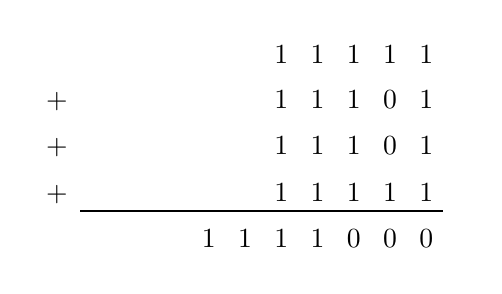
\begin{tikzpicture}[
    every node/.style={column sep=.5mm,row sep=1mm}]
    \matrix (m) [matrix of math nodes,
        nodes in empty cells,
        %nodes=draw
    ] 
    {
        &  &  &  &  &  &  &  & 1 & 1 & 1 & 1 & 1 &     \\
    +   &  &  &  &  &  &  &  & 1 & 1 & 1 & 0 & 1 &            \\
    +   &  &  &  &  &  &  &  & 1 & 1 & 1 & 0 & 1 &            \\
    +   &  &  &  &  &  &  &  & 1 & 1 & 1 & 1 & 1 &            \\
        &  &  &  &  &  & 1 & 1 & 1 & 1 & 0 & 0 &  0&            \\                                                  
    };

    \draw[-,color=black,semithick] (m-4-2.south west) -- (m-4-13.south east);

\end{tikzpicture}
\end{equation*}

The following example demonstrates the entire process by using different colors to distinguish each column and the corresponding carries they produce. Note that the last two digits in the sum are colored black, as they do not result from any specific column but are instead generated solely from the carries.

\begin{equation*}
\begin{tikzpicture}[
    row 1/.style={font=\textsl,font=\tiny, anchor=mid,
        inner sep=1.5pt},
    row 2/.style={font=\textsl,font=\tiny, anchor=mid,
        inner sep=1.5pt},
    row 3/.style={font=\textsl,font=\tiny, anchor=mid,
        inner sep=1.5pt},
    every node/.style={column sep=.5mm,row sep=1mm}]
    \matrix (m) [matrix of math nodes,
        nodes in empty cells,
        %nodes=draw
    ] 
    {
        &   &   &   &   &   &  \textcolor{YellowOrange}{1} &  \textcolor{YellowOrange}{0} &  &  &  &  &   &            \\
        &   &   &   &   &   &  & \textcolor{Purple}{1} & \textcolor{Purple}{0} &  & \textcolor{red}{1}  &  &   &            \\
        &   &   &   &   &   &  &  & \textcolor{Green}{1}  & \textcolor{Green}{1}  & \textcolor{blue}{1}  & \textcolor{blue}{0}  &   &            \\
        &  &  &  &  &  &  &  & \textcolor{YellowOrange}{1} & \textcolor{Purple}{1} & \textcolor{Green}{1}  & \textcolor{red}{1}  & \textcolor{blue}{1} &     \\
    +   &  &  &  &  &  &  &  &  \textcolor{YellowOrange}{1} & \textcolor{Purple}{1} & \textcolor{Green}{1}  & \textcolor{red}{0} & \textcolor{blue}{1}  &            \\
    +   &  &  &  &  &  &  &  &  \textcolor{YellowOrange}{1} & \textcolor{Purple}{1} & \textcolor{Green}{1}  & \textcolor{red}{0}  & \textcolor{blue}{1}  &            \\
    +   &  &  &  &  &  &  &  &  \textcolor{YellowOrange}{1} & \textcolor{Purple}{1} & \textcolor{Green}{1}  & \textcolor{red}{1}  & \textcolor{blue}{1}  &            \\
        &  &  &  &  &  & 1 & 1 &  \textcolor{YellowOrange}{1} & \textcolor{Purple}{1} & \textcolor{Green}{0}  & \textcolor{red}{0}  & \textcolor{blue}{1}  &            \\                                                  
    };

    \draw[-,color=black,semithick] (m-7-2.south west) -- (m-7-13.south east);

\end{tikzpicture}
\end{equation*}

\subsubsection*{Method 2: Direct Summation and Simplification}
We will illustrate the second method using the same example. In the previous case, we carried the actual binary number to the next columns. In this method, we write down 0 if the sum is even and 1 if the sum is odd. Every time a sum a multiple of 2, we carry a 1 to the next columns, and then continue this process for each column, including the carries in the calculation of that column.

\textbf{Step 1: Add the Rightmost Column}\newline
Add bits in column 1 (from counting from MSB):

$$
1+1+1+1=100_2 \quad(\text { which is binary for } 4)
$$
Reading the result from LSB to MSB
\begin{itemize}
    \item write down the 0
    \item carry a 1 for the first multiple of 2
    \item carry a 1 for the second multiple of 2
\end{itemize}
This results in


\begin{equation*}
\begin{tikzpicture}[
    row 1/.style={font=\textsl,font=\tiny, anchor=mid,
        inner sep=1.5pt},
    row 2/.style={font=\textsl,font=\tiny, anchor=mid,
        inner sep=1.5pt},
    row 3/.style={font=\textsl,font=\tiny, anchor=mid,
        inner sep=1.5pt},
    every node/.style={column sep=.5mm,row sep=1mm}]
    \matrix (m) [matrix of math nodes,
        nodes in empty cells,
        %nodes=draw
    ] 
    {
        &   &   &   &   &   &  &  &  &  &  &  &   &            \\
        &   &   &   &   &   &  &  &  &  &  & 1 &   &            \\
        &   &   &   &   &   &  &  & &  &  & 1 &   &            \\
        &  &  &  &  &  &  &  & 1 & 1 & 1 & 1 & 1 &     \\
    +   &  &  &  &  &  &  &  & 1 & 1 & 1 & 0 & 1 &            \\
    +   &  &  &  &  &  &  &  & 1 & 1 & 1 & 0 & 1 &            \\
    +   &  &  &  &  &  &  &  & 1 & 1 & 1 & 1 & 1 &            \\
        &  &  &  &  &  &  &  &  &  &  &  & 0 &            \\                                                  
    };

    \draw[-,color=black,semithick] (m-7-2.south west) -- (m-7-13.south east);

\end{tikzpicture}
\end{equation*}

\textbf{Step 2: Add the Second Column from the Right}\newline
Add bits in column 2 (from counting from MSB):

$$
1+1+1+1=100_2 \quad(\text { which is binary for } 4)
$$
Reading the result from LSB to MSB
\begin{itemize}
    \item write down the 0
    \item carry a 1 for the first multiple of 2
    \item carry a 1 for the second multiple of 2
\end{itemize}
This results in


\begin{equation*}
\begin{tikzpicture}[
    row 1/.style={font=\textsl,font=\tiny, anchor=mid,
        inner sep=1.5pt},
    row 2/.style={font=\textsl,font=\tiny, anchor=mid,
        inner sep=1.5pt},
    row 3/.style={font=\textsl,font=\tiny, anchor=mid,
        inner sep=1.5pt},
    every node/.style={column sep=.5mm,row sep=1mm}]
    \matrix (m) [matrix of math nodes,
        nodes in empty cells,
        %nodes=draw
    ] 
    {
        &   &   &   &   &   &  &  &  &  &  &  &   &            \\
        &   &   &   &   &   &  &  &  &  & 1  &  &   &            \\
        &   &   &   &   &   &  &  & &  & 1 &  &   &            \\
        &  &  &  &  &  &  &  & 1 & 1 & 1 & 1 & 1 &     \\
    +   &  &  &  &  &  &  &  & 1 & 1 & 1 & 0 & 1 &            \\
    +   &  &  &  &  &  &  &  & 1 & 1 & 1 & 0 & 1 &            \\
    +   &  &  &  &  &  &  &  & 1 & 1 & 1 & 1 & 1 &            \\
        &  &  &  &  &  &  &  &  &  &  & 0 & 0 &            \\                                                  
    };

    \draw[-,color=black,semithick] (m-7-2.south west) -- (m-7-13.south east);

\end{tikzpicture}
\end{equation*}

\newpage

\textbf{Step 3: Add the Third Column from the Right}
Add bits in column 3 (from counting from MSB):

$$
1+1+1+1+1+1=110_2 \quad(\text { which is binary for } 6)
$$
Reading the result from LSB to MSB
\begin{itemize}
    \item write down the 0
    \item carry a 1 for the first multiple of 2
    \item carry a 1 for the second multiple of 2
    \item carry a 1 for the third multiple of 2
\end{itemize}
This results in


\begin{equation*}
\begin{tikzpicture}[
    row 1/.style={font=\textsl,font=\tiny, anchor=mid,
        inner sep=1.5pt},
    row 2/.style={font=\textsl,font=\tiny, anchor=mid,
        inner sep=1.5pt},
    row 3/.style={font=\textsl,font=\tiny, anchor=mid,
        inner sep=1.5pt},
    every node/.style={column sep=.5mm,row sep=1mm}]
    \matrix (m) [matrix of math nodes,
        nodes in empty cells,
        %nodes=draw
    ] 
    {
        &   &   &   &   &   &  &  &  & 1 &  &  &   &            \\
        &   &   &   &   &   &  &  &  & 1 &   &  &   &            \\
        &   &   &   &   &   &  &  & & 1 &  &  &   &            \\
        &  &  &  &  &  &  &  & 1 & 1 & 1 & 1 & 1 &     \\
    +   &  &  &  &  &  &  &  & 1 & 1 & 1 & 0 & 1 &            \\
    +   &  &  &  &  &  &  &  & 1 & 1 & 1 & 0 & 1 &            \\
    +   &  &  &  &  &  &  &  & 1 & 1 & 1 & 1 & 1 &            \\
        &  &  &  &  &  &  &  &  &  & 0 & 0 & 0 &            \\                                                  
    };

    \draw[-,color=black,semithick] (m-7-2.south west) -- (m-7-13.south east);

\end{tikzpicture}
\end{equation*}

\textbf{Step 4: Add the Fourth Column from the Right}\newline
Add bits in column 4 (from counting from MSB):

$$
1+1+1+1+1+1+1=111_2 \quad(\text { which is binary for } 7)
$$
Reading the result from LSB to MSB
\begin{itemize}
    \item write down the 1
    \item carry a 1 for the first multiple of 2
    \item carry a 1 for the second multiple of 2
    \item carry a 1 for the third multiple of 2
\end{itemize}
This results in


\begin{equation*}
\begin{tikzpicture}[
    row 1/.style={font=\textsl,font=\tiny, anchor=mid,
        inner sep=1.5pt},
    row 2/.style={font=\textsl,font=\tiny, anchor=mid,
        inner sep=1.5pt},
    row 3/.style={font=\textsl,font=\tiny, anchor=mid,
        inner sep=1.5pt},
    every node/.style={column sep=.5mm,row sep=1mm}]
    \matrix (m) [matrix of math nodes,
        nodes in empty cells,
        %nodes=draw
    ] 
    {
        &   &   &   &   &   &  &  & 1 &  &  &  &   &            \\
        &   &   &   &   &   &  &  & 1 &  &   &  &   &            \\
        &   &   &   &   &   &  &  & 1 &  &  &  &   &            \\
        &  &  &  &  &  &  &  & 1 & 1 & 1 & 1 & 1 &     \\
    +   &  &  &  &  &  &  &  & 1 & 1 & 1 & 0 & 1 &            \\
    +   &  &  &  &  &  &  &  & 1 & 1 & 1 & 0 & 1 &            \\
    +   &  &  &  &  &  &  &  & 1 & 1 & 1 & 1 & 1 &            \\
        &  &  &  &  &  &  &  &  & 1 & 0 & 0 & 0 &            \\                                                  
    };

    \draw[-,color=black,semithick] (m-7-2.south west) -- (m-7-13.south east);

\end{tikzpicture}
\end{equation*}


\textbf{Step 5: Add the Leftmost Column}\newline
Add bits in leftmost column):

$$
1+1+1+1+1+1+1=111_2 \quad(\text { which is binary for } 7)
$$
Reading the result from LSB to MSB
\begin{itemize}
    \item write down the result in binary, i.e. 1 1 1
\end{itemize}
This results in


\begin{equation*}
\begin{tikzpicture}[
    row 1/.style={font=\textsl,font=\tiny, anchor=mid,
        inner sep=1.5pt},
    row 2/.style={font=\textsl,font=\tiny, anchor=mid,
        inner sep=1.5pt},
    row 3/.style={font=\textsl,font=\tiny, anchor=mid,
        inner sep=1.5pt},
    every node/.style={column sep=.5mm,row sep=1mm}]
    \matrix (m) [matrix of math nodes,
        nodes in empty cells,
        %nodes=draw
    ] 
    {
        &   &   &   &   &   &  &  &  &  &  &  &   &            \\
        &   &   &   &   &   &  &  &  &  &   &  &   &            \\
        &   &   &   &   &   &  &  & &  &  &  &   &            \\
        &  &  &  &  &  &  &  & 1 & 1 & 1 & 1 & 1 &     \\
    +   &  &  &  &  &  &  &  & 1 & 1 & 1 & 0 & 1 &            \\
    +   &  &  &  &  &  &  &  & 1 & 1 & 1 & 0 & 1 &            \\
    +   &  &  &  &  &  &  &  & 1 & 1 & 1 & 1 & 1 &            \\
        &  &  &  &  &  & 1 & 1 & 1 & 1 & 0 & 0 & 0 &            \\                                                  
    };

    \draw[-,color=black,semithick] (m-7-2.south west) -- (m-7-13.south east);
\end{tikzpicture}
\end{equation*}

which corresponds to the result we obtained above. While not demonstrated explicitly here, subtraction works in a similar fashion.

By using one of these methods for handling multiple carries, allow us to also multiply two binary numbers.



\subsection*{Multiplication in Binary}
Multiplication in binary is technically easier than multiplication in decimal. In binary operations, we work exclusively with two digits: 0 and 1. This means that both the the multiplier\footnote{The "multiplicand" is the number that has to be multiplied, and the "multiplier" is the number by which it is multiplied.} and multiplicand consist of 0's and 1' (and so does the multiplicand). The process of finding the binary product is analogous to traditional multiplication in the decimal system. The four five steps involved in multiplying binary digits are:

\[
\begin{aligned}
& 0 \times 0=0 \\
& 0 \times 1=0 \\
& 1 \times 0=0 \\
& 1 \times 1=1 \\
& 1 \times 10_2 = 10_2 \quad \left( \text{multiplying by base } 10_2 \text{ adds a 0 to the end} \right)
\end{aligned}
\]

The last step means that $101_2 \times 10_2 = 1010_2$ which is analogous to the decimal case: $143_{10} \times 10_{10} = 1430_{10}$.

We will illustrate the process by supplying a couple of examples.

\newpage

\begin{example}


\begin{equation*}
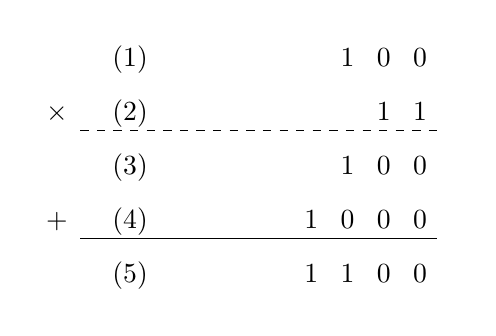
\begin{tikzpicture}[
    every node/.style={column sep=.5mm,row sep=1mm}]
    \matrix (m) [matrix of math nodes,
        nodes in empty cells,
        %nodes=draw
    ] 
    {
        &   &  (1) &   &   &   &  &  &  &  & 1 & 0 & 0  &            \\
     \times   &   & (2)  &   &   &   &  &  &  &  &   & 1 &  1 &            \\
        &   & (3)  &   &   &   &  &  & &  & 1 & 0 & 0  &            \\
       + &  & (4) &  &  &  &  &  &  & 1 & 0 & 0 & 0 &     \\
        &  & (5) &  &  &  &  &  &  & 1 & 1 & 0 & 0 &            \\                                                  
    };

    \draw[dashed, color=black, semithick] (m-2-2.south west) -- (m-2-13.south east);
    \draw[-,color=black,semithick] (m-4-2.south west) -- (m-4-13.south east);
    \end{tikzpicture}
\end{equation*}

Here are the steps:

\begin{itemize}
    \item Multiply the multiplicand (line 1) by the LSB of the multiplier (line 2), which in this case is 1.
    \item Record this result in line 3.
    \item Append a 0 to line 4 to account for the shift to the next power of 2 in the multiplier.
    \item Multiply the multiplicand (line 1) by the next bit of the multiplier (line 2), which is also 1 in this case.
    \item Add this result to line 4, after the 0 you appended earlier.
    \item Finally, sum the values in lines 3 and 4, as outlined in the previous section, to obtain the final result in line 5.
\end{itemize}
\end{example}

We offer two additional examples:

\begin{example}

\begin{equation*}
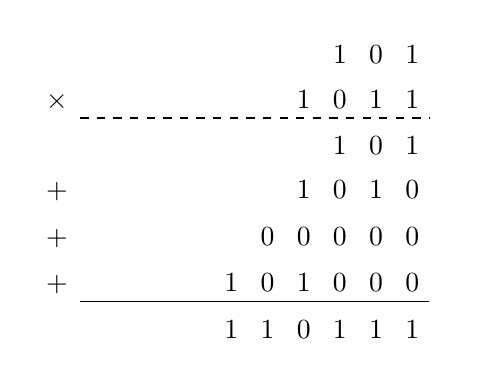
\begin{tikzpicture}[
    every node/.style={column sep=.5mm,row sep=1mm}]
    \matrix (m) [matrix of math nodes,
        nodes in empty cells,
        %nodes=draw
    ] 
    {
        &   &   &   &   &   &  &  &  &  & 1 & 0 & 1  &            \\
     \times   &   &   &   &   &   &  &  &  & 1 &  0 & 1 &  1 &            \\
        &   &   &   &   &   &  &  & &  & 1 & 0 & 1  &            \\
       + &  &  &  &  &  &  &  &  & 1 & 0 & 1 & 0 &     \\
       + &  &  &  &  &  &  &  & 0 & 0 & 0 & 0 & 0 &            \\               
       + &  &  &  &  &  &  & 1 & 0 & 1 & 0 & 0 & 0 &     \\
        &  &  &  &  &  &  & 1 & 1 & 0 & 1 & 1 & 1 &            \\                                        
    };

    \draw[dashed, color=black, semithick] (m-2-2.south west) -- (m-2-13.south east);
    \draw[-,color=black,semithick] (m-6-2.south west) -- (m-6-13.south east);
    \end{tikzpicture}
\end{equation*}
    
\end{example}

\begin{example}
\label{ex3.1}
\begin{equation*}
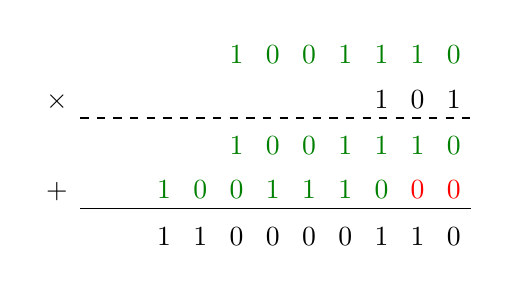
\begin{tikzpicture}[
    every node/.style={column sep=.5mm,row sep=1mm}]
    \matrix (m) [matrix of math nodes,
        nodes in empty cells,
        %nodes=draw
    ] 
    {
        &   &   &   &   &   & \textcolor{Green}{1} & \textcolor{Green}{0} & \textcolor{Green}{0} & \textcolor{Green}{1} & \textcolor{Green}{1} & \textcolor{Green}{1} & \textcolor{Green}{0}  &            \\
     \times   &   &   &   &   &   &  &  &  &  &  1 & 0 &  1 &            \\
        &   &   &   &   &   & \textcolor{Green}{1} & \textcolor{Green}{0} & \textcolor{Green}{0} & \textcolor{Green}{1} & \textcolor{Green}{1} & \textcolor{Green}{1} & \textcolor{Green}{0}   &            \\
       + &  &  &  & \textcolor{Green}{1} & \textcolor{Green}{0} & \textcolor{Green}{0} & \textcolor{Green}{1} & \textcolor{Green}{1} & \textcolor{Green}{1} & \textcolor{Green}{0} & \textcolor{Red}{0} & \textcolor{Red}{0} &            \\             
        &  &  &  & 1 & 1 & 0 & 0 & 0 & 0 & 1 & 1 & 0 &     \\                                     
    };

    \draw[dashed, color=black, semithick] (m-2-2.south west) -- (m-2-13.south east);
    \draw[-,color=black,semithick] (m-4-2.south west) -- (m-4-13.south east);
    \end{tikzpicture}
\end{equation*}
    
\end{example}

In \autoref{ex3.1} notice that we omitted the row of zeroes that the second value of the multiplier would have produced, and notice even further that we added two 0's before restating the multiplicand in the sum.

Binary multiplication, like binary addition, is a core operation in computer arithmetic. By breaking the process down into manageable steps—multiplying individual bits and then summing the results—it becomes clear how similar it is to the multiplication methods we use in the decimal system. The main difference is the simplicity and efficiency of working within the binary system, where only the digits 0 and 1 are involved.

We notice how binary multiplication builds on binary addition. Each step, involving shifts and sums, essentially consists of repeated additions adjusted by powers of two. A strong grasp of binary addition naturally leads to a better understanding of binary multiplication and its applications.

\section{Octal and Hexadecimal}
Octal is a base-8 numbering system that uses the digits 0 through 7. It is closely related to binary, which is a base-2 system. The connection between the two lies in how easily binary numbers can be converted to octal and vice versa. Each octal digit corresponds to exactly three binary digits (bits), making conversions straightforward. For example, the binary number `110` converts directly to the octal digit `6`. Because of this close relationship, octal is often used as a shorthand for binary in computing, particularly in contexts where grouping binary digits in sets of three simplifies reading and interpreting binary data.

\[
\begin{aligned}
12_8 &= 1 \cdot 8^1 + 2 \cdot 8^0  = 10_{10} \\
3021_8 & = 3 \cdot 8^3 + 0 \cdot 8^2 + 2 \cdot 8^1 + 1 \cdot 8^0 = 1553_{10}
\end{aligned}
\]

Since \(8\) is \(2^3\), we can express it in binary:

\[
\begin{aligned}
3 & \rightarrow \textcolor{Green}{011} \\
0 & \rightarrow \textcolor{YellowOrange}{000} \\
2 & \rightarrow \textcolor{blue}{010} \\
1 & \rightarrow \textcolor{red}{001} \\
\end{aligned}
\]

\[
\text{Thus, } 3021_8 = \textcolor{Green}{011}\textcolor{YellowOrange}{000} \textcolor{blue}{010}\textcolor{red}{001}_2 = \textcolor{Green}{11}\textcolor{YellowOrange}{000} \textcolor{blue}{010}\textcolor{red}{001}_2
\]

We obtain the final result by removing leading zeros.

Hexadecimal is a base-16 numbering system that uses sixteen distinct symbols: the digits 0-9 and the letters A-F, where A represents 10, B represents 11, and so on up to F, which represents 15. Hexadecimal is closely related to binary because each hexadecimal digit corresponds exactly to four binary digits (bits). This direct relationship makes it easy to convert between the two systems. For example, the hexadecimal digit `A` translates to the binary sequence `1010`. Due to this efficiency in grouping, hexadecimal is often used in computing as a more compact and readable way to represent binary data, particularly in areas like memory addresses and colour codes in web design.

\[
\begin{aligned}
123_{16} &= 1 \cdot 16^2 + 2 \cdot 16^1 + 3 \cdot 16^0  = 256 + 32 + 3 = 291_{10} \\
A2E_{16} & = 10 \cdot 16^2 + 2 \cdot 16^1 + 14 \cdot 16^0 = 2560 + 32 + 14 = 2606_{10}
\end{aligned}
\]

Since \(16\) is \(2^4\), we can, for instance, express $A2E_{16}$ in binary:

\[
\begin{aligned}
A & \rightarrow 1010 \\
2 & \rightarrow 0010 \\
E & \rightarrow 1110 \\
\end{aligned}
\]

\[
\text{Thus, } A2E_{16} = 101000101110_2
\]

Similarly we get $5EB52_{16}$ as

\[
\begin{aligned}
5 & \rightarrow 0101 \\
E & \rightarrow 1110 \\
B & \rightarrow 1011 \\
5 & \rightarrow 0101 \\
2 & \rightarrow 0010 \\
\end{aligned}
\]

\[
\text{Thus, } 5EB52_{16} = 01011110101101010010_2
\]

Again, notice that we removed the leading 0's from $5_{16}$ when writing the result.

\section{Converting Between Systems}

Understanding how to convert numbers between binary, decimal, octal, and hexadecimal systems is essential in computer science and digital electronics. Each system is a different base, and each has its own applications. Here's a step-by-step guide to help you convert numbers from one system to another.

\subsection*{Decimal to Binary Conversion}
To convert a decimal number to binary:
\begin{enumerate}
    \item Divide the decimal number by 2.
    \item Record the remainder (it will be 0 or 1).
    \item Divide the quotient by 2 and record the remainder.
    \item Repeat until the quotient is 0.
    \item The binary number is the sequence of remainders read from bottom to top.
\end{enumerate}

\begin{example} Convert \(23_{10}\) to binary.

\begin{solution}

\[
\begin{aligned}
23 \div 2 & = 11 \quad \text{remainder } 1 \\
11 \div 2 & = 5 \quad \text{remainder } 1 \\
5 \div 2 & = 2 \quad \text{remainder } 1 \\
2 \div 2 & = 1 \quad \text{remainder } 0 \\
1 \div 2 & = 0 \quad \text{remainder } 1 \\
\end{aligned}
\]
Thus, \(23_{10} = 10111_2\). \end{solution}
\end{example}

\subsection*{Decimal to Octal Conversion}
To convert a decimal number to octal:
\begin{enumerate}
    \item Divide the decimal number by 8.
    \item Record the remainder.
    \item Divide the quotient by 8 and record the remainder.
    \item Repeat until the quotient is 0.
    \item The octal number is the sequence of remainders read from bottom to top.
\end{enumerate}

\begin{example}Convert \(78_{10}\) to octal.

\begin{solution}
    


\[
\begin{aligned}
78 \div 8 & = 9 \quad \text{remainder } 6 \\
9 \div 8 & = 1 \quad \text{remainder } 1 \\
1 \div 8 & = 0 \quad \text{remainder } 1 \\
\end{aligned}
\]
Thus, \(78_{10} = 116_8\). \end{solution}
    
\end{example}

\subsection*{Decimal to Hexadecimal Conversion}
To convert a decimal number to hexadecimal:
\begin{enumerate}
    \item Divide the decimal number by 16.
    \item Record the remainder (use A, B, C, D, E, F for remainders 10, 11, 12, 13, 14, 15 respectively).
    \item Divide the quotient by 16 and record the remainder.
    \item Repeat until the quotient is 0.
    \item The hexadecimal number is the sequence of remainders read from bottom to top.
\end{enumerate}

\begin{example}Convert \(255_{10}\) to hexadecimal.

\begin{solution}
    
\[
\begin{aligned}
255 \div 16 & = 15 \quad \text{remainder } 15 \quad (\text{F}) \\
15 \div 16 & = 0 \quad \text{remainder } 15 \quad (\text{F}) \\
\end{aligned}
\]
Thus, \(255_{10} = FF_{16}\).\end{solution}

\end{example}


\subsection*{Binary to Decimal Conversion}
To convert a binary number to decimal:
\begin{enumerate}
    \item Multiply each bit by 2 raised to the power of its position, starting from 0 on the right.
    \item Sum all the products.
\end{enumerate}

Notice that this amounts to the method outlined above about binary expansion.

\begin{example} Convert \(1101_2\) to decimal.

\begin{solution}
    

\[
\begin{aligned}
1 \cdot 2^3 + 1 \cdot 2^2 + 0 \cdot 2^1 + 1 \cdot 2^0 & = 8 + 4 + 0 + 1 = 13_{10}
\end{aligned}
\] \end{solution}

\end{example}

\subsection*{Binary to Octal Conversion}
To convert a binary number to octal:
\begin{enumerate}
    \item Group the binary digits into sets of three, starting from the right. Add leading zeros if necessary.
    \item Convert each group of three binary digits to its octal equivalent.
\end{enumerate}

\begin{example}Convert \(110110_2\) to octal.

\begin{solution}
\[
\begin{aligned}
110 & \rightarrow 6 \\
110 & \rightarrow 6 \\
\end{aligned}
\]
Thus, \(110110_2 = 66_8\). \end{solution}

\end{example}

\subsection*{Binary to Hexadecimal Conversion}
To convert a binary number to hexadecimal:
\begin{enumerate}
    \item Group the binary digits into sets of four, starting from the right. Add leading zeros if necessary.
    \item Convert each group of four binary digits to its hexadecimal equivalent.
\end{enumerate}

\begin{example}Convert \(10110101_2\) to hexadecimal.

\begin{solution}
\[
\begin{aligned}
1011 & \rightarrow B \\
0101 & \rightarrow 5 \\
\end{aligned}
\]
Thus, \(10110101_2 = B5_{16}\). \end{solution}

\end{example}

\subsection*{Octal to Binary Conversion}
To convert an octal number to binary:
\begin{enumerate}
    \item Convert each octal digit to its 3-bit binary equivalent.
\end{enumerate}

\begin{example}Convert \(57_8\) to binary.

\begin{solution}
\[
\begin{aligned}
5 & \rightarrow 101 \\
7 & \rightarrow 111 \\
\end{aligned}
\]
Thus, \(57_8 = 101111_2\). \end{solution}

\end{example}

\subsection*{Octal to Decimal Conversion}
To convert an octal number to decimal:
\begin{enumerate}
    \item Multiply each digit by 8 raised to the power of its position, starting from 0 on the right.
    \item Sum all the products.
\end{enumerate}

\begin{example}Convert \(157_8\) to decimal.

\begin{solution}
    
\[
\begin{aligned}
1 \cdot 8^2 + 5 \cdot 8^1 + 7 \cdot 8^0 & = 64 + 40 + 7 = 111_{10}
\end{aligned}
\] \end{solution}

\end{example}

\subsection*{Octal to Hexadecimal Conversion}
To convert an octal number to hexadecimal:
\begin{enumerate}
    \item First, convert the octal number to binary.
    \item Then, convert the binary number to hexadecimal by grouping the binary digits in sets of four.
\end{enumerate}

\begin{example}Convert \(157_8\) to hexadecimal.

\begin{solution}

\[
\begin{aligned}
1 & \rightarrow 001 \\
5 & \rightarrow 101 \\
7 & \rightarrow 111 \\
\end{aligned}
\]
Thus, \(157_8 = 001101111_2 = 6F_{16}\). \end{solution}
\end{example}

\subsection*{Hexadecimal to Binary Conversion}
To convert a hexadecimal number to binary:
\begin{enumerate}
    \item Convert each hexadecimal digit to its 4-bit binary equivalent.
\end{enumerate}

\begin{example}Convert \(2B_{16}\) to binary.

\begin{solution}
    


\[
\begin{aligned}
2 & \rightarrow 0010 \\
B & \rightarrow 1011 \\
\end{aligned}
\]
Thus, \(2B_{16} = 00101011_2\).\end{solution}

\end{example}

\subsection*{Hexadecimal to Decimal Conversion}
To convert a hexadecimal number to decimal:
\begin{enumerate}
    \item Multiply each digit by 16 raised to the power of its position, starting from 0 on the right.
    \item Sum all the products.
\end{enumerate}

\begin{example}Convert \(2B_{16}\) to decimal.

\begin{solution}
\[
\begin{aligned}
2 \cdot 16^1 + 11 \cdot 16^0 & = 32 + 11 = 43_{10}
\end{aligned}
\] \end{solution}
\end{example}

\subsection*{Hexadecimal to Octal Conversion}
To convert a hexadecimal number to octal:
\begin{enumerate}
    \item First, convert the hexadecimal number to binary.
    \item Then, convert the binary number to octal by grouping the binary digits in sets of three.
\end{enumerate}

\begin{example}Convert \(2B_16\) to octal.

\begin{solution}

\[
\begin{aligned}
2 & \rightarrow 0010 \\
B & \rightarrow 1011 \\
\end{aligned}
\]
Thus, \(2B_{16} = 00101011_2 = 53_8\). \end{solution}

\end{example}

\subsection*{Final Thoughts on Conversion}
The concept of expansion plays a central role in these conversions. Whether you are expanding a decimal number into its binary, octal, or hexadecimal form, or converting a binary number into its octal or hexadecimal equivalent, you are more or less expressing the number in terms of powers of the base. The expansion method is essentially the same for each system as it boils down to dividing by the highest power of the base recursively:

$$
\begin{aligned}
7562_{10} & =1 \cdot 16^3+3466=1 \cdot 16^3+13 \cdot 16^2+138 \\
& =\textcolor{red}{1} \cdot 16^3+ \textcolor{blue}{13} \cdot 16^2+\textcolor{YellowOrange}{8} \cdot 16^1+\textcolor{Green}{10} \cdot 16^0=\textcolor{red}{1} \, \textcolor{blue}{D} \, \textcolor{YellowOrange}{8} \, \textcolor{Green}{A}
\end{aligned}
$$

By understanding these expansions and the relationships between these number systems, you can efficiently switch between them, allowing you to represent and manipulate data in the most suitable format for any given situation.

\chapter{Combinatorics and Probability Theory}
\label{chap:ch4}
Imagine you are tasked with forming teams of 3 for a semester project in a class of 45 students. Initially, the order in which you choose the team members does not matter, so you are just concerned with combinations. The number of ways to form a team of 3 from 45 students comes out to 14,190 possibilities!

The following semester introduces the students to Scrum project management, where each team must have three specific roles: Scrum Master, Product Owner, and Development Team. This small change, specifying roles, suddenly transforms the problem from a simple \textit{combination} into a \textit{permutation}. Now, the number of possible ways to assign these roles leaps to 85,140!

Frustrated by the sheer number of options, the 45 students throw a party to relax. Being well-mannered, they decide that everyone should shake hands with every other person exactly once. After a few minutes, they calculate the total number of handshakes — 990. The students are once again surprised by how something as simple as shaking hands can add up so quickly.

As the night progresses, one student proposes a fun game — a random drawing for five door prizes, each unique. With 45 students in attendance and only five prizes available, the chance of winning nothing becomes a concerning 89 per cent. The students quickly realize that the odds are not in their favor.

Not ready to give up on their luck, a smaller group decides to flip a coin 10 times, with the hope of landing exactly five heads to win the game. However, when they learn that the probability of this happening is only about 25 per cent, their spirits dampen further.

The students conclude that rather than relying on chance, it is time to dive deeper into understanding combinatorics and probability theory. Armed with this knowledge, they can better predict outcomes and avoid future disappointments at both parties and project planning.

\section{Sample Space and Events}
\label{sec:sample_space}
A \textbf{random experiment }is one that can lead to different outcomes, even when repeated under the same conditions. This randomness is a fundamental aspect of many engineering tasks.

Think of it this way: Let us say you are testing the speed of a website under different conditions. Sometimes it loads quickly, and other times it is slower. Even if you are using the same code and server, things like network traffic or server load make the results vary each time. 

\begin{definition}{Random Experiment}
    A random experiment is one that can give different results, even if you do everything the same each time.
\end{definition}

Or, imagine you are measuring the signal strength in a wireless device. You might get slightly different readings each time because of things like interference or small changes in the environment.

This randomness shows up all over the place, from software performance tests to electrical engineering experiments. It is important to expect it and include it in your thinking. Otherwise, you might make decisions based on incomplete or misleading data. When you account for random variation, you can make smarter predictions and designs.

To model and analyze a random experiment, it is crucial to understand the set of possible outcomes that can occur. In probability theory, this set is called the \textbf{sample space}, denoted by \( S \). A sample space can be either \textbf{discrete} (consisting of a finite or countably infinite set of outcomes) or \textbf{continuous} (containing an interval of real numbers). The exact definition of a sample space often depends on the objectives of the analysis.

An \textbf{outcome} is a single possible result of the random experiment, and an \textbf{event} is any subset of the sample space, which may consist of one or more outcomes. Below are some examples to illustrate these concepts:

\begin{example}[ Network Latency] \\
Consider an experiment where you measure the latency of data packets in a network. The sample space can be defined based on the type of measurements:
\begin{itemize}
    \item If latency is measured as a positive real number, the sample space is continuous: 
    \[
    S = \{ x \mid x > 0 \}.
    \]
    \item If it is known that latency ranges between 10 and 100 milliseconds, the sample space can be refined to:
    \[
    S = \{ x \mid 10 \leq x \leq 100 \}.
    \]
    \item If the objective is to categorize latency as low, medium, or high, the sample space becomes discrete:
    \[
    S = \{\text{low}, \text{medium}, \text{high}\}.
    \]
    \item For a simple evaluation of whether the latency meets a standard threshold, the sample space can be reduced to:
    \[
    S = \{\text{pass}, \text{fail}\}.
    \]
\end{itemize}
Each outcome in these sample spaces represents a single possible latency measurement, and events can be defined as sets of outcomes, such as "latency is high."

\end{example}

Understanding the nature of sample spaces, outcomes, and events is fundamental in probability, as it allows us to define and work with probabilities of complex scenarios in various engineering contexts. Let us summarise these key concepts:

\begin{definition}{Sample Spaces, Outcomes, and Events}
    \textbf{Sample Space:} The set of all possible outcomes of a random experiment is called the sample space, denoted by \( S \). Outcomes can be discrete or continuous, depending on the nature of the experiment.
    
    \textbf{Outcome:} A single possible result of a random experiment.
    
    \textbf{Event:} Any subset of the sample space, which may consist of one or more outcomes.
\end{definition}

\begin{example} Software Release Testing \\
    Imagine a software testing process where each test case can either pass or fail. The sample space for a single test case is discrete and can be represented as:
    \[
    S = \{\text{pass}, \text{fail}\}.
    \]
    If you run three test cases, the combined sample space for all possible outcomes is:
    \begin{align*}
    S = \{&(\text{pass, pass, pass}), (\text{pass, pass, fail}), (\text{pass, fail, pass}), \\
    &(\text{pass, fail, fail}), (\text{fail, pass, pass}), (\text{fail, pass, fail}), \\
    &(\text{fail, fail, pass}), (\text{fail, fail, fail})\}.
    \end{align*}
    This sample space includes all sequences of outcomes for the three tests.
    
    \begin{itemize}
        \item The total number of possible outcomes is \( 2^3 = 8 \).
        \item An event could be defined as "at least one test fails," which would include outcomes like \(\text{(fail, pass, pass)}\), \(\text{(pass, fail, fail)}\), and others where at least one test fails.
    \end{itemize}
    
    \end{example}
    

\begin{example} Component Quality in Manufacturing \\
A company manufactures electronic components, and each component is tested for compliance with quality standards. The test can return one of three outcomes: \texttt{pass}, \texttt{marginal}, or \texttt{fail}. The sample space is:
\[
S = \{\text{pass}, \text{marginal}, \text{fail}\}.
\]
\textbf{Event:} Suppose we are interested in the event that a component does not pass the quality test. This event is a set of outcomes:
\[
E = \{\text{marginal}, \text{fail}\}.
\]
\end{example}

This means that all the operations we have defined on sets translate directly into operations on events:
\begin{itemize}
    \item $A \cup B$: the event that at least one of $A$ or $B$ occurs.
    \item $A \cap B$: the event that both $A$ and $B$ occur together.
    \item $\skoverline{A}$ or $A^c$: the event that $A$ does not occur.
    \item $A \setminus B$ or $A - B$: the event that $A$ occurs but $B$ does not.
    \item $A \Delta B$ or $A \oplus B$: the event that either $A$ or $B$ occurs, but not both (symmetric difference).
\end{itemize}

Thus, probability theory builds directly on set theory: probability assigns a numerical measure to these subsets of the sample space. In the next chapter, we will see how this measure is defined and used to reason about uncertainty.

We can summarise the considerations of this section in the following table:

\begin{table}[h]
    \centering
    \renewcommand{\arraystretch}{1.5} % Adjust this value for desired spacing
    \begin{tabular}{|c|c|c|c|}
    \hline
    \textbf{Operation} & \textbf{Boolean Algebra} & \textbf{Logic} & \textbf{Set Theory} \\
    \hline
    \texttt{NOT} & $\skoverline{x}$ & $\neg x$ & $A^c$ or $A'$\\
    \hline
    \texttt{OR} & $+$ & $\vee$ & $\cup$ \\
    \hline
    \texttt{AND} & $\cdot$ & $\wedge$ & $\cap$ \\
    \hline
    \texttt{NAND} & $\skoverline{x \cdot y}$ & $\neg (x \wedge y)$ & $(A \cap B)^c$ or \(\skoverline{A \cap B}\)\\
    \hline
    \texttt{NOR} & $\skoverline{x + y}$ & $\neg (x \vee y)$ & $(A \cup B)^c$ or \(\skoverline{A \cup B}\) \\
    \hline
    \texttt{XOR} (Symmetric Difference) & $x \oplus y$ & $(x \wedge \neg y) \vee (\neg x \wedge y)$ & $A \triangle B$ or \(A \oplus B\) \\
    \hline
    Difference & $x \cdot \skoverline{y}$ & $x \wedge \neg y$ & $A - B$ or \( A \setminus B \) \\
    \hline
    \end{tabular}
    \caption{Comparison of Operators in Boolean Algebra, Logic, and Set Theory}
\end{table}

In this book, we will use the notation $A^c$ to denote the complement of the set $A$, which includes all elements not in $A$.

\section{Counting Principles}

In many problems across mathematics, computer science, and engineering, determining the number of ways certain events can occur is important. Whether you're arranging elements, selecting groups, or navigating through complex scenarios, counting techniques provide the foundational tools to solve these problems. These techniques go beyond simple arithmetic and allow us to tackle questions like:

\begin{itemize}
    \item How many ways can we arrange a set of objects?
    \item In how many different paths can a process unfold?
    \item What is the probability of a specific event occurring given multiple possibilities?
\end{itemize}

Counting techniques, such as permutations, combinations, and the multiplication rule, help us quantify these possibilities systematically.

\subsection*{Multiplication Rule}

We start out by discussing the most basic counting principle: the \textbf{multiplication rule}:

\begin{theorem}[Multiplication Rule]
    Let an operation be described as a sequence of $k$ steps. Assume the following conditions:
    
    \begin{itemize}
        \item There are $n_1$ ways to complete step 1.
        \item There are $n_2$ ways to complete step 2 for each way of completing step 1.
        \item There are $n_3$ ways to complete step 3 for each way of completing step 2, and so on.
    \end{itemize}
    
    Then, the total number of ways to complete the entire operation is given by:
    
    \[
    n_1 \times n_2 \times \cdots \times n_k.
    \]
\end{theorem}
    
\begin{example}
    Suppose you are choosing a meal at a restaurant. You have the following options:
        
    \begin{itemize}
            \item 3 choices for the main course.
            \item 4 choices for the side dish.
            \item 2 choices for the drink.
    \end{itemize}
        
    Using the multiplication rule, the total number of ways to choose a meal is:
        
    \[
        3 \times 4 \times 2 = 24.
    \]
        
    Therefore, there are 24 different meal combinations available.
\end{example}

\begin{example} Automobile Options

An automobile manufacturer provides vehicles equipped with selected
options. Each vehicle is ordered

\begin{itemize}
    \item With or without an automatic transmission
    \item With or without a sunroof
    \item With one of three choices of a stereo system
    \item With one of four exterior colors
\end{itemize}

If the sample space consists of the set of all possible vehicle types, what is the number of outcomes in the sample space?
\end{example}

\begin{solution}
Using the multiplication rule, we can calculate the total number of possible vehicle types by multiplying the number of choices for each option:

\begin{itemize}
    \item 2 choices for the transmission (with or without automatic transmission)
    \item 2 choices for the sunroof (with or without sunroof)
    \item 3 choices for the stereo system
    \item 4 choices for the exterior color
\end{itemize}

Therefore, the total number of possible vehicle types is:

\[
2 \times 2 \times 3 \times 4 = 48
\]

So, there are 48 different possible vehicle types in the sample space.
\end{solution}

\subsection*{Replacement and Order in Counting}

Next we turn to an important distinction between with and without replacement in counting principles:

\begin{definition}[Counting with and without Replacement]
    When counting the number of ways to select objects from a set, two common scenarios are:

    \begin{itemize}
        \item \textbf{With Replacement}: An object can be selected more than once.
        \item \textbf{Without Replacement}: Once an object is selected, it cannot be chosen again.
    \end{itemize}
    \end{definition}
    
\begin{example}
    Suppose you have a bag containing 5 different colored balls. You draw 2 balls:
\begin{itemize}
    \item \textbf{With Replacement}: The first ball is placed back in the bag before drawing the second. There are \(5 \times 5 = 25\) possible outcomes.
    \item \textbf{Without Replacement}: The first ball is not placed back, so the number of outcomes is \(5 \times 4 = 20\).
\end{itemize}
\end{example}

\begin{example}
    Three people are drawing cards one after another from a standard deck of 52 cards. The goal is to find the Ace of Spades. Let's examine the two scenarios: with replacement and without replacement.

    \textbf{Without Replacement}

    In this scenario, each card drawn is not put back into the deck, reducing the total number of cards available after each draw.
    \begin{itemize}
        \item First Draw: The first person has a $\frac{1}{52}$ chance of drawing the Ace of Spades.
        \item Second Draw: If the first person does not draw the Ace of Spades, there are now 51 cards left, and the second person has a $\frac{1}{51}$ chance of drawing the Ace of Spades.
        \item Third Draw: If the Ace of Spades has not been drawn by the first two people, the third person has a $\frac{1}{50}$ chance of drawing it.
    \end{itemize}
    
    The probabilities change with each draw because the total number of cards decreases, and previously drawn cards are not available.
    
    \textbf{With Replacement}

    In this scenario, each card drawn is returned to the deck and reshuffled before the next person draws. This keeps the total number of cards constant.
    \begin{itemize}
        \item First Draw: The first person has a $\frac{1}{52}$ chance of drawing the Ace of Spades.
        \item Second Draw: Since the card is replaced and shuffled back into the deck, the second person also has a $\frac{1}{52}$ chance of drawing the Ace of Spades.
        \item Third Draw: Similarly, the third person has a $\frac{1}{52}$ chance of drawing the Ace of Spades.
    \end{itemize}
    
    The probabilities remain the same for each draw because the deck is reset to its original state after each draw.

\end{example}

\begin{example}
    Imagine you have a group of 5 students: Alice, Bob, Charlie, David, and Eve. You need to select 2 of them for different scenarios, illustrating when the order of selection matters and when it does not.
    \begin{itemize}
        \item \textbf{Order Matters}: Selecting Alice as Captain and Bob as Assistant Captain is a different outcome than selecting Bob as Captain and Alice as Assistant Captain.
        \end{itemize}
    Now, imagine you are simply selecting 2 students to form a study group with no specific roles assigned. Here, the order does not matter.
    \begin{itemize}
        \item \textbf{Order does not matters:}  Choosing Alice and Bob is considered the same outcome as choosing Bob and Alice; there is no distinction between the two orders since there are no assigned roles.
    \end{itemize}
    \label{ex:order_matters}
\end{example}

\autoref{ex:order_matters} illustrates the distinction between \textit{permutations} and \textit{combinations}, two fundamental counting principles that are widely used in probability theory and combinatorics.

\begin{definition}[Permutation and Combination]
    \begin{itemize}
        \item \textbf{Permutation (order matters)}: Different sequences are counted as distinct outcomes, leading to a higher count.
        \item \textbf{Combination (order does not matter)}: Sequences are treated as identical, resulting in a lower count.
    \end{itemize}
\end{definition}

We will first discuss permutations, which are used when the order of selection matters.

\subsection*{Permutations}

Consider a set of elements, such as $S=\{a, b, c\}$. A permutation of the elements is an ordered sequence of the elements. For example, $a b c, a c b, b a c, b c a, c a b$, and $c b a$ are all of the permutations of the elements of $S$.

\begin{proposition}[Permutations of \(n\) Distinct Objects]
    The number of ordered arrangements (permutations) of $n$ distinct objects is
    \[
    n! = n \cdot (n-1) \cdot \dots \cdot 2 \cdot 1.
    \]
\end{proposition}

This outcome is a direct application of the multiplication rule. To form a permutation, you start by choosing an element for the first position from the total of $n$ elements. Next, you choose an element for the second position from the remaining $n-1$ elements, then for the third position from the remaining $n-2$ elements, and continue this way until all positions are filled. Such arrangements are often called linear permutations.

\begin{example}
    It is said that any shuffling of a deck of card has only happened once in history. This is because the number of ways to shuffle a deck of 52 cards is \(52!\), which is an astronomically large number.

    \[52! \approx 8.07 \times 10^{67}\]
\end{example}

\begin{example}
    Suppose you have 5 different books on a shelf. You want to rearrange them in a different order. The number of ways to rearrange the books is
    \[5! = 5 \times 4 \times 3 \times 2 \times 1 = 120\]
\end{example}

There are cases where we are only interested in arranging a subset of elements from a larger set. The formula for counting these arrangements also derives from the multiplication rule.

\begin{theorem}[Permutations of Subsets]
    For integers $n \ge r \ge 0$, the number of ordered selections of $r$ distinct objects from $n$ distinct objects is
    \[
    P_r^n = P(n,r) = n \cdot (n-1) \cdots (n-r+1) = \frac{n!}{(n-r)!}.
    \]
\end{theorem}

\begin{example}
    Suppose you have 5 different books on a shelf, and you want to rearrange 3 of them in a different order. The number of ways to rearrange the 3 books is
    \[
    P_3^5=5 \times 4 \times 3 = 60
    \]
\end{example}

\begin{example}
    There are 10 entries in a contest. Only three will win, $1^{\text {st }}, 2^{\text {nd }}$, or $3^{\text {rd }}$ prize. What are the possible results?
\end{example}
\begin{solution}
    The number of ways to award the prizes is the number of permutations of 3 objects selected from 10, which is
    \[
    P_3^{10}= \frac{10!}{(10-3)!}=\frac{10!}{7!} = 10 \times 9 \times 8 = 720
    \]
    Therefore, there are 720 possible outcomes for awarding the prizes.
\end{solution}

\subsection*{Combinations}

When the order of selection does not matter, we use the concept of combinations. Combinations are used when we are interested in selecting a subset of elements from a larger set without regard to the order in which they are selected. Let is start out with a couple of examples to illustrate the concept of combinations.

\begin{example}
    Suppose you have a group of 5 students: Alice, Bob, Charlie, David, and Eve. You need to select 2 of them to form a study group. The order in which you select the students does not matter. The possible combinations are:
    \begin{itemize}
        \item Alice and Bob
        \item Alice and Charlie
        \item Alice and David
        \item Alice and Eve
        \item Bob and Charlie
        \item Bob and David
        \item Bob and Eve
        \item Charlie and David
        \item Charlie and Eve
        \item David and Eve
    \end{itemize}
    The order of the students in the study group does not matter, so the combinations are considered identical.
\end{example}

\begin{example}
    Maria has three tickets for a concert. She'd like to use one of the tickets herself. She could then offer the other two tickets to any of four friends (Ann, Beth, Chris, Dave). How many ways can 2 people be selected from 4 to go to a concert?
\end{example}

\begin{example}
A circuit board has four different locations in which a component can be placed. If three identical components are to be placed on the board, how many different designs are possible?
\end{example}

\begin{solution}
    Since you can only place one component in each slot, placing a component in any slot immediately restricts the choices for the next component.
        
    \begin{enumerate}
        \item Fill slots 1, 2, and 3.
        \item Fill slots 1, 2, and 4.
        \item Fill slots 1, 3, and 4.
        \item Fill slots 2, 3, and 4.
    \end{enumerate}
\end{solution}

These examples illustrate the concept of combinations, where the order of selection does not matter. The formula for combinations is derived from the permutation formula by dividing out the number of ways to arrange the $r$ elements.

\begin{theorem}[Combinations]
    The number of combinations of $r$ elements selected from a set of $n$ different elements is given by
    \[
    C_r^n = \binom{n}{r} = \frac{n!}{r!(n-r)!}
    \]
\end{theorem}

This is also sometimes referred to as the \textbf{binomial coefficient}, denoted by $\binom{n}{r}$, which is read as "n choose r". It is called the binomial coefficient because it appears in the binomial theorem, which expands the powers of a binomial expression:

\begin{theorem}[Binomial Theorem]
    In algebra, the binomial coefficient is used to expand powers of binomials. According to the binomial theorem

$$
(a+b)^n=\sum_{k=0}^n\binom{n}{k} a^k b^{n-k}
$$

\end{theorem}

The theorem states that the expansion of the binomial expression $(a+b)^n$ is the sum of the terms $\binom{n}{k} a^k b^{n-k}$ for $k=0,1,2,\ldots,n$. The binomial coefficient $\binom{n}{k}$ gives the number of ways to choose $k$ elements from a set of $n$ elements. We will place no more emphasis on the binomial theorem here, but it is a fundamental concept in algebra and combinatorics, and is widely used in probability theory.

We will conclude our discussion of counting principles with principles of counting with replacement.

\begin{proposition}[With replacement]
For selections from $n$ types:
\begin{itemize}
    \item \textbf{Ordered with replacement}: $n^r$ outcomes.
    \item \textbf{Unordered with replacement}: $\displaystyle \binom{n+r-1}{r}$ outcomes. % (stars and bars)
\end{itemize}
\end{proposition}

\section{Basic Probability}
Probability quantifies the likelihood or chance that an outcome of a random experiment will occur. For instance, when you hear, “The chance of rain today is 30\%,” it expresses our belief about the likelihood of rain. Probabilities are numbers assigned to outcomes, ranging from 0 to 1 (or equivalently, from 0\% to 100\%). A probability of 0 means the outcome will not happen, while a probability of 1 means it will happen for sure.

Probabilities can be interpreted in different ways:

\begin{itemize}
    \item \textbf{Objective (or Classical) Probability}: Often referred to as classical probability, this approach is used when outcomes are equally likely, such as in rolling a fair die or flipping a coin. Probabilities are assigned based on the assumption that each outcome has an equal chance of occurring. For example, when rolling a fair six-sided die, the probability of rolling a 3 is \( \frac{1}{6} \) because there are 6 equally likely outcomes (1, 2, 3, 4, 5, 6), and only one of them is a 3. The probability is the same for all observers.
        
    \item \textbf{Relative Frequency (Empirical Probability)}: Empirical probability is based on observations from experiments rather than theoretical calculations. For example, if a software tester runs a stress test on a server 100 times and it crashes 7 times, the empirical probability of a crash is \( \frac{7}{100} = 0.07 \). This approach relies on actual data rather than assumptions or intuition.
        
    \item \textbf{Subjective Probability}: This reflects our personal belief or degree of confidence in an outcome. Different people might assign different probabilities to the same event based on their knowledge or perspective. You and your friends discuss Denmark’s chances of winning the World Cup. Based on recent performance and team strength, you estimate a 10\% chance. However, a more optimistic friend assigns a 20\% chance, while another gives only 5\%, considering stronger competitors. This illustrates subjective probability, where each person's estimate varies based on personal beliefs and biases rather than objective data.
    

\end{itemize}

When assigning probabilities, it’s essential that the sum of all probabilities in an experiment equals 1, ensuring consistency with the relative frequency interpretation.

We start by establishing the Axioms of Probability, which lay the foundation for how probabilities are assigned to events. These axioms define the basic properties that every probability measure must satisfy.
    
\begin{axiom}[Axioms of Probability]
    \begin{itemize}
        \item \textbf{Axiom 1:} For any event \(A\), \( 0 \leq P(A) \leq 1 \).
        \item \textbf{Axiom 2:} Probability of the sample space \(S\) is \(P(S) = 1\).
        \item \textbf{Axiom 3:} If \(A_1, A_2, A_3, \cdots\) are disjoint events, then \(P\left(A_1 \cup A_2 \cup A_3 \cdots\right) = P\left(A_1\right) + P\left(A_2\right) + P\left(A_3\right) + \cdots\)
    \end{itemize}
\end{axiom}

The property that \( 0 \leq P(A) \leq 1 \) is equivalent to the requirement that a relative frequency must be between 0 and 1. The property that \( P(S) = 1 \) is a consequence of the fact that an outcome from the sample space occurs on every trial of an experiment. Consequently, the relative frequency of \( S \) is 1. Property 3 implies that if the events \( A_1 \) and \( A_2 \) have no outcomes in common, the relative frequency of outcomes in \( A_1 \cup A_2 \) is the sum of the relative frequencies of the outcomes in \( A_1 \) and \( A_2 \).

In the next sections we will see more about the probability of events and how to calculate them.

\subsection*{Probability of an Event}
The probability of an event is a measure of the likelihood that the event will occur. It is denoted by \( P(A) \), where \( A \) is the event. The probability of an event ranges from 0 to 1, where 0 indicates that the event will not occur, and 1 indicates that the event will occur for sure.

\begin{definition}[Probability of an Event]
    The probability of an event \( A \), denoted by \( P(A) \), is the likelihood that event \( A \) will occur. It is defined as the ratio of the number of favorable outcomes to the total number of outcomes in the sample space.
    \[
    P(A) = \frac{\text{Number of favorable outcomes}}{\text{Total number of outcomes}}
    \]
\end{definition}

\begin{example}
    Suppose you are testing a software module with 10 different test cases. Out of these, 3 test cases are known to fail due to a bug. If you randomly select one test case to run, what is the probability that the selected test case will fail?
\end{example}

\begin{solution}
    Here, the event $A$ is "the test case fails."
\begin{itemize}
    \item Number of favorable outcomes (failing test cases) $=3$
    \item Total number of outcomes (total test cases) $=10$
\end{itemize}

Using the formula:

$$
P(A)=\frac{\text { Number of favorable outcomes }}{\text { Total number of outcomes }}=\frac{3}{10}=0.3
$$


Therefore, the probability that a randomly selected test case will fail is 0.3 , indicating that there is a $30 \%$ chance of failure.

\end{solution}

\begin{example}
    Imagine a software development environment where you have 50 files, consisting of 20 Python scripts, 15 Java files, and 15 configuration files. If you randomly select one file to edit, what is the probability that the file is a Python script?
\end{example}

\begin{solution}
Here, the event $A$ is "the selected file is a Python script."
\begin{itemize}
    \item Number of favorable outcomes (Python scripts) $=20$
    \item Total number of outcomes (total files) $=50$
\end{itemize}

Using the formula:

$$
P(A)=\frac{\text { Number of favorable outcomes }}{\text { Total number of outcomes }}=\frac{20}{50}=0.4
$$

Thus, the probability of selecting a Python script is 0.4 , meaning there is a $40 \%$ chance of choosing a Python file from the set.

\end{solution}

\section{Probability of Joint Events and Set Operations}
Joint events are formed by applying basic set operations to individual events. Commonly, we encounter unions of events, such as $A \cup B$; intersections of events, such as $A \cap B$; and complements of events, such as $A^c$. These combined events are often of particular interest, and their probabilities can frequently be derived from the probabilities of the individual events that compose them. Understanding these set operations is essential for accurately calculating the probability of joint events. In this section, we will explore how unions of events and other set operations can be used to determine the probabilities of more complex events.

When dealing with events, the intersection represents \texttt{AND} while the union represents \texttt{OR} The probability of the intersection of events $A$ and $B$, denoted as $P(A \cap B)$, can also be expressed as $P(A, B)$ or $P(A B)$.

From the axioms of probability, we can derive the following rules of probabilities:

\begin{theorem}{Rules of Probability}
    \begin{itemize}
        \item \textbf{Complement Rule:} The probability of the complement of event $A$ is
    
        \[
        P(A^c) = 1 - P(A)
        \]

        \item \textbf{Empty Set Rule:} The probability of the empty set is 0, i.e.,
        
        \[P(\emptyset) = 0\]
        
        \item \textbf{Addition Rule:} For any two events $A$ and $B$, the probability of the union of events $A$ and $B$ is given by
        \[
        P(A \cup B) = P(A) + P(B) - P(A \cap B)
        \]

        \item \textbf{Difference Rule:} The probability of the difference between events $A$ and $B$ is given by
        \[
        P(A-B)=P(A)-P(A \cap B)
        \]
        \item \textbf{Subset Rule:} If $A$ is a subset of $B$ ($A \subset B$), then
        \[P(A) \leq P(B)\].
    \end{itemize}
\end{theorem}

We can obtain the Complement Rule by noting:

\begin{align*}
    1 &= P(S) & \text{(axiom 2)} \\
      &= P(A \cup A^c) & \text{(definition of complement)} \\
      &= P(A) + P(A^c) & \text{(since } A \text{ and } A^c \text{ are disjoint)}
\end{align*}

Since $\emptyset=S^c$, we can apply part the Complement Rule to deduce that $P(\emptyset)=1-P(S)=0$. This is intuitive because, by definition, an event occurs when the outcome of the random experiment is part of that event. However, since the empty set contains no elements, no outcome of the experiment can ever belong to it, making its probability zero.

The Difference Rule can be obtained by showing that $P(A)=P(A \cap B)+P(A-B)$. Note that the two sets $A \cap B$ and $A-B$ are disjoint and their union is $A$. Thus, by the third axiom of probability

\begin{align*}
    P(A) &= P\left((A \cap B) \cup (A - B)\right) & \text{(since } A = (A \cap B) \cup (A - B)) \\
         &= P(A \cap B) + P(A - B) & \text{(since } A \cap B \text{ and } A - B \text{ are disjoint)}
    \end{align*}
    

The Addition Rule we obtain by noting that $A$ and $B-A$ are disjoint sets and their union is $A \cup B$. Thus,

\begin{align*}
    P(A \cup B) &= P(A \cup (B - A)) && (\text{since } A \cup B = A \cup (B - A)) \\
                &= P(A) + P(B - A) && (\text{since } A \text{ and } B - A \text{ are disjoint}) \\
                &= P(A) + P(B) - P(A \cap B) && (\text{by part the Difference Rule})
    \end{align*}
    
And finally the Subset Rule is a direct consequence of the fact that if $A \subset B$, then $B$ can be written as the union of $A$ and $B-A$. Since $A$ and $B-A$ are disjoint, we have $P(B)=P(A)+P(B-A) \geq P(A)$.

We conclude this section with a few examples illustrating the application of these rules to calculate probabilities of joint events.

\begin{example}
    A company has bid on two large construction projects. The company president believes that the probability of winning the first contract is 0.6, the probability of winning the second contract is 0.4, and the probability of winning both contracts is 0.2.

    \begin{enumerate}[label=(\alph*)]
        \item What is the probability that the company wins at least one contract?
        \item What is the probability that the company wins the first contract but not the second contract?
        \item What is the probability that the company wins neither contract?
        \item What is the probability that the company wins exactly one contract?
    \end{enumerate}
\end{example}

\begin{solution}
    Let $A$ be the event that the company wins the first contract, and $B$ be the event that the company wins the second contract. Given:
    \begin{itemize}
        \item $P(A) = 0.6$
        \item $P(B) = 0.4$
        \item $P(A \cap B) = 0.2$
    \end{itemize}
    
    \begin{enumerate}[label=(\alph*)]
        \item The probability that the company wins at least one contract is the probability of the union of events $A$ and $B$. Using the Addition Rule:
        
        \begin{align*}
            P(A \cup B) &= P(A) + P(B) - P(A \cap B) \\
                        &= 0.6 + 0.4 - 0.2 \\
                        &= 0.8
        \end{align*}
        
        Therefore, the probability that the company wins at least one contract is 0.8.
        
        \item The probability that the company wins the first contract but not the second contract is the probability of the difference between events $A$ and $B$. Using the Difference Rule:
        
        \begin{align*}
            P(A - B) &= P(A) - P(A \cap B) \\
                    &= 0.6 - 0.2 \\
                    &= 0.4
        \end{align*}
        
        Therefore, the probability that the company wins the first contract but not the second contract is 0.4.
        
        \item The probability that the company wins neither contract is the probability of the complement of the union of events $A$ and $B$. Using the Complement Rule:
        
        \begin{align*}
            P((A \cup B)^c) &= 1 - P(A \cup B) \\
                                    &= 1 - 0.8 \\
                                    &= 0.2
        \end{align*}
        
        Therefore, the probability that the company wins neither contract is 0.2.
        
        \item The probability that the company wins exactly one contract is the probability of the difference between the union of events $A$ and $B$ and the intersection of events $A$ and $B$. Using the Difference Rule:
            
            \begin{align*}
                P((A \cup B) - (A \cap B)) &= P(A \cup B) - P(A \cap B) \\
                                            &= 0.8 - 0.2 \\
                                            &= 0.6
            \end{align*}
            So, the probability that the company wins exactly one contract is 0.6.
            \end{enumerate}
\end{solution}

\begin{example}
    \begin{itemize}
    \item There is a 60 percent chance that it will rain today.
    \item There is a 50 percent chance that it will rain tomorrow.
    \item There is a 30 percent chance that it does not rain either day.
    \end{itemize}
    
\begin{enumerate}[label=(\alph*)]
    \item The probability that it will rain today or tomorrow
    \item The probability that it will rain today and tomorrow.
    \item The probability that it will rain today but not tomorrow.
    \item The probability that it either will rain today or tomorrow, but not both.
\end{enumerate}
    
\begin{solution}
\begin{enumerate}[label=(\alph*)]
    \item     Let \( A \) be the event that it rains today, and \( B \) be the event that it rains tomorrow.
        
    Given:
    \begin{align*}
        P(A \cup B) &= 1 - P\left((A \cup B)^c\right) \quad &\text{by the Complement Rule} \\
                &= 1 - P\left(A^c \cap B^c\right) \quad &\text{by De Morgan's Law} \\
                &= 1 - 0.3 \\
                &= 0.7
    \end{align*}
            
        
    Therefore, the probability that it will rain today or tomorrow is \( 0.7 \).

    \item The probability that it will rain today and tomorrow: this is $P(A \cap B)$. To find this we note that
    \begin{align*}
    P(A \cap B) &= P(A) + P(B) - P(A \cup B) \\
                &= 0.6 + 0.5 - 0.7 \\
                &= 0.4
    \end{align*}

    \item The probability that it will rain today but not tomorrow: this is $P\left(A \cap B^c\right)$.

    \begin{align*}
        P(A \cap B^c) &= P(A - B) \\
                      &= P(A) - P(A \cap B) \\
                      &= 0.6 - 0.4 \\
                      &= 0.2
        \end{align*}
        
    \item The probability that it either will rain today or tomorrow but not both: this is $P(A-B)+P(B-A)$. We have already found $P(A-B)=.2$. Similarly, we can find $P(B-A)$:
    
    \begin{align*}
        P(B-A) & =P(B)-P(B \cap A) \\
        & =0.5-0.4 \\
        & =0.1
        \end{align*}
    Thus,
    \begin{align*}
        P(A-B)+P(B-A) &= 0.2+0.1 \\
                      &= 0.3
    \end{align*}
\end{enumerate}
\end{solution}
\end{example}

\chapter{Conditional Probability and Bayes' Theorem}\label{chap:ch5}

In this section, we introduce more fundamental concepts of probability. We begin with \textbf{conditional probability}, which assesses the likelihood of an event occurring \textit{given} that another event has already taken place. Building on this, we introduce \textbf{the multiplication rule}, a key principle for determining the probability of multiple events happening in sequence. Next, we explore \textbf{the law of total probability}, which allows us to break down and calculate probabilities across different scenarios or partitions of the sample space. To further distinguish how events interact, we examine \textbf{dependent and independent events}, clarifying how the occurrence of one event influences or does not influence another. 

Finally, we look into \textbf{Bayes' Theorem}, a powerful tool for updating probabilities in light of new evidence.

\section{Conditional Probability}
Consider the following scenario: in a particular population, 5\% of individuals have a specific medical condition. Therefore, the probability that a randomly selected person has the condition is 5\%:

\[
P(D) = 0.05,
\]

where \( D \) represents the event that a person has the disease. This probability \( P(D) \) is known as the \textit{prior probability}, as it reflects our initial belief about the likelihood of the event before any additional information is obtained.

Now, imagine selecting a random person and being informed that they have tested positive for the disease. With this additional information, how should we update the probability that the person actually has the disease? In other words, what is the probability that a person has the disease given that they tested positive? Let \( T \) denote the event that a person tests positive. This conditional probability is expressed as:

\[
P(D \mid T),
\]

which represents the probability of \( D \) occurring given that \( T \) has occurred. This updated probability \( P(D \mid T) \) is known as the \textit{posterior probability}, as it reflects our revised belief about the likelihood of the event after taking the new evidence into account. Intuitively, it is reasonable to expect that \( P(D \mid T) \) is greater than the prior probability \( P(D) \). However, what is the exact value of \( P(D \mid T) \)? Before introducing a general formula, let us consider a simple example.

\begin{example}
I roll a fair die. Let \( A \) be the event that the outcome is a prime number, i.e., \( A = \{2, 3, 5\} \). Also, let \( B \) be the event that the outcome is greater than or equal to 3, i.e., \( B = \{3, 4, 5\} \). 

\begin{enumerate}[label=(\alph*)]
    \item What is the probability of \( A \), \( P(A) \)?
    \item What is the probability of \( A \) given \( B \), \( P(A \mid B) \)?
\end{enumerate}

\end{example}

\begin{solution}
    \begin{enumerate}[label=(\alph*)]
        \item The probability of \( A \) is the number of outcomes in \( A \) divided by the total number of outcomes. Since there are 3 prime numbers and 6 possible outcomes, we have:
    
        \begin{align*}
        P(A) &= \frac{3}{6} = \frac{1}{2}
        \end{align*}
    
        \item The probability of \( A \) given \( B \) is the number of outcomes in the intersection of \( A \) and \( B \) divided by the number of outcomes in \( B \). Since the outcomes in the intersection of \( A \) and \( B \) are \(\{3, 5\}\) and the outcomes in \( B \) are \(\{3, 4, 5\}\), we have:
    
        \begin{align*}
        P(A \mid B) &=\frac{|A \cap B|}{|B|} = \frac{|\{3,5\}|}{|\{3,4, 5\}|} = \frac{2}{3}
        \end{align*}

    \end{enumerate}
\end{solution}

Having understood the basic example, we can now generalize the approach to derive a more universal formula for conditional probability. Starting from the specific case, we can manipulate the expression by dividing both the numerator and the denominator by the total number of possible outcomes, \( |S| \), as shown below:

\[
P(A \mid B) = \frac{|A \cap B|}{|B|} = \frac{\frac{|A \cap B|}{|S|}}{\frac{|B|}{|S|}} = \frac{P(A \cap B)}{P(B)}
\]

\textbf{Explanation:}

\begin{itemize}
    \item \textbf{Numerator:} \( |A \cap B| \) represents the number of outcomes where both events \( A \) and \( B \) occur. Dividing by \( |S| \) converts this count into a probability, \( P(A \cap B) \).
    \item \textbf{Denominator:} \( |B| \) is the number of outcomes where event \( B \) occurs. Similarly, dividing by \( |S| \) yields the probability of event \( B \), denoted as \( P(B) \).
\end{itemize}

Thus, the conditional probability \( P(A \mid B) \) can be expressed as the ratio of the joint probability of \( A \) and \( B \) to the probability of \( B \).

While the above derivation assumes a finite sample space with equally likely outcomes, the resulting formula is remarkably general. It holds true regardless of whether the sample space is finite or infinite, and whether the outcomes are equally likely or not. This universality makes the formula a cornerstone of probability theory.

\begin{definition}[Conditional Probability]
For any two events \( A \) and \( B \) with \( P(B) > 0 \), the conditional probability of \( A \) given \( B \) is defined as:
\[
P(A \mid B) = \frac{P(A \cap B)}{P(B)}, \qquad P(B) > 0
\]
\end{definition}

Here is the intuition behind the formula. When we know that event \( B \) has occurred, we effectively eliminate all outcomes that are not part of \( B \). This reduction transforms our original sample space into the subset \( B \).

Within this new, restricted sample space \( B \), the only way for event \( A \) to occur is if the outcome lies in the intersection of \( A \) and \( B \), denoted by \( A \cap B \). To determine the conditional probability \( P(A \mid B) \), we calculate the ratio of the probability of both \( A \) and \( B \) occurring to the probability of \( B \) occurring alone. Mathematically, this is expressed as:

\[
P(A \mid B) = \frac{P(A \cap B)}{P(B)}
\]

This formulation ensures that the probabilities within the new sample space \( B \) are normalized, meaning the total probability sums to 1. For instance, consider the conditional probability of \( B \) given \( B \):

\[
P(B \mid B) = \frac{P(B \cap B)}{P(B)} = \frac{P(B)}{P(B)} = 1
\]

This result intuitively confirms that if \( B \) has occurred, the probability of \( B \) occurring is certain, i.e., 1.

Note that the conditional probability \( P(A \mid B) \) is undefined when \( P(B) = 0 \). This scenario implies that event \( B \) never occurs. Since conditional probability relies on the occurrence of \( B \), if \( B \) has a probability of zero, there are no outcomes in the sample space to condition upon. Therefore, discussing the probability of \( A \) given \( B \) becomes meaningless in this context.

We can also formulate the axioms of probability in terms of conditional probability. The axioms of probability are as follows:

\begin{axiom}[Axioms of Conditional Probability]
    \begin{itemize}
        \item \textbf{Axiom 1:} For any event \(A\), \( 0 \leq P(A\mid B) \leq 1 \).
        \item \textbf{Axiom 2:} Conditional probability of $B$ given $B$ is 1, i.e., $P(B \mid B)=1$.
        \item \textbf{Axiom 3:} If \(A_1, A_2, A_3, \cdots\) are disjoint events, then $P\left(A_1 \cup A_2 \cup A_3 \cdots \mid B\right)=P\left(A_1 \mid B\right)+P\left(A_2 \mid B\right)+P\left(A_3 \mid B\right)+\cdots$
    \end{itemize}
\end{axiom}

And we are also able to derive other rules of conditional probability from these axioms:

\begin{theorem}{Rules of Conditional Probability}
    \begin{itemize}
        \item \textbf{Complement Rule:} The probability of the complement of event $A$ given $C$ is
    
        \[
        P\left(\skoverline{A} \mid C\right)=1-P(A \mid C)
        \]

        \item \textbf{Empty Set Rule:} The probability of the empty set given some event $C$ is 0, i.e.,
        
        \[P(\emptyset \mid C) = 0\]
        
        \item \textbf{Addition Rule:} For any two events $A$ and $B$, the probability of the union of events $A$ and $B$ given another event $C$ is
        \[
        P(A \cup B \mid C)=P(A \mid C)+P(B \mid C)-P(A \cap B \mid C)
        \]

        \item \textbf{Difference Rule:} The probability of the difference between events $A$ and $B$ given another event $C$ is
        \[
            P(A-B \mid C)=P(A \mid C)-P(A \cap B \mid C)
        \]
        \item \textbf{Subset Rule:} If $A \subset B$, then
        \[
        P(A \mid C) \leq P(B \mid C)
        \]
    \end{itemize}
\end{theorem}

The following example illustrates the application of conditional probability and introduces the concept of \textbf{contingency tables} as well as \textbf{false positives} and \textbf{false negatives}.

\begin{example}
    A researcher aims to assess the effectiveness of a diagnostic test designed to detect renal disease in patients with high blood pressure. To achieve this, she conducts the test on a sample of 137 patients, categorized as follows:

\begin{itemize}
    \item \textbf{67 patients} with a confirmed diagnosis of renal disease.
    \item \textbf{70 patients} who are known to be healthy (i.e., do not have renal disease).
\end{itemize}

The diagnostic test produces one of two possible outcomes for each patient:

\begin{itemize}
    \item \textbf{Positive}: Indicates that the patient has renal disease.
    \item \textbf{Negative}: Indicates that the patient does not have renal disease.
\end{itemize}

The findings are summarised in the following contingency table:

    \begin{tabular}{lrrr} 
        & \multicolumn{2}{c}{ Test Results } & \\
        Truth & Positive & Negative & Total \\
        Renal Disease & 44 & 23 & 67 \\
        Healthy & 10 & 60 & 70 \\
        Total & 54 & 83 & 137
        \end{tabular}
        
    In this experiment:


        \begin{itemize}
            \item \textbf{True Positives}: Patients who have renal disease and tested positive.
            \item \textbf{False Negatives}: Patients who have renal disease but tested negative.
            \item \textbf{False Positives}: Healthy patients who tested positive.
            \item \textbf{True Negatives}: Healthy patients who tested negative.
        \end{itemize}
    
        Determine the following probabilities:
        \begin{enumerate}[label=(\alph*)]
            \item The Probability of Renal Disease, $P(D)$.
            \item The Probability of Renal Disease,  \( P(T^+) \).
            \item The Probability of Renal Disease,  \( P(T^-) \).
            \item If a person has renal disease, what is the probability that they test positive for the disease?
            \item Determine the probability that a patient has renal disease given a positive test result, \( P(\text{Renal Disease} \mid \text{Positive}) \).
            \item Determine the probability that a patient does not have renal disease given a negative test result, \( P(\text{Healthy} \mid \text{Negative}) \).
            \item Assess the overall accuracy of the diagnostic test.
        \end{enumerate}
        label{ex:renal-disease}
\end{example}

\begin{solution}
    Using the contingency table, we can calculate the following probabilities:

    \begin{enumerate}[label=(\alph*)]
        \item \textbf{Probability of Renal Disease, \( P(D) \)}:
        \begin{align*}
        P(D) &= \frac{\text{Number of patients with renal disease}}{\text{Total number of patients}} \\
        &= \frac{67}{137} \approx 0.4883 \text{ or } 48.83\%
        \end{align*}
        
        \item \textbf{Probability of a Positive Test, \( P(T^+) \)}:
        \begin{align*}
        P(T^+) &= \frac{\text{Number of positive tests}}{\text{Total number of patients}} \\
        &= \frac{54}{137} \approx 0.3942 \text{ or } 39.42\%
        \end{align*}
        
        \item \textbf{Probability of a Negative Test, \( P(T^-) \)}:
        \begin{align*}
        P(T^-) &= \frac{\text{Number of negative tests}}{\text{Total number of patients}} \\
        &= \frac{80}{137} \approx 0.6058 \text{ or } 60.58\%
        \end{align*}


        \item \textbf{Probability of a Positive Test Given Renal Disease, \( P(T^+ \mid D) \)}:
        \begin{align*}
            P(T+\mid D)=\frac{44}{67} \approx 0.6567
        \end{align*}

        \item \textbf{Probability of Renal Disease Given a Positive Test, \( P(D \mid T^+) \)}:
        \begin{align*}
        P(D \mid T^+) &= \frac{P(D \cap T^+)}{P(T^+)} \\
        &= \frac{44}{54}=\frac{22}{27} \approx 0.8148
        \end{align*}

        \item \textbf{Probability of Being Healthy Given a Negative Test, \( P(\text{Healthy} \mid T^-) \)}:
        \begin{align*}
        P(\text{Healthy} \mid T^-) &= \frac{P(\text{Healthy} \cap T^-)}{P(T^-)} \\
        &= \frac{60}{83} \approx 0.7229
        \end{align*}

        \item \textbf{Overall Accuracy of the Diagnostic Test}:
        The overall accuracy of the diagnostic test is the proportion of correct diagnoses, i.e., the sum of true positives and true negatives divided by the total number of patients:
        \begin{align*}
            \text{Overall Accuracy} =\frac{44+60}{137}=\frac{104}{137} \approx 0.7591
        \end{align*}
    \end{enumerate}


The results of the analysis indicate that the diagnostic test has a high probability of correctly identifying patients with renal disease (81.48\%). However, the test is less effective at identifying healthy patients, with a probability of 72.29\%. The overall accuracy of the test is 75.91\%, reflecting the proportion of correct diagnoses across all patients.
\end{solution}

Here’s a classic probability puzzle known as the Two-Child Problem.This scenario has appeared in various forms in the literature, each with subtle twists that lead to different results. Before looking at the calculations, take a moment to make your own predictions — you might be surprised by the outcomes!

\begin{example}
    Consider a family with two children, and we are interested in the possible gender combinations of the children. The sample space for this situation is:

\[
S = \{(G, G), (G, O), (B, O), (O, O)\}
\]

where \( G \) represents a girl and \( O \) represents a child that is not a girl. For simplicity, we assume that all four outcomes are equally likely.

\begin{enumerate}[label=(\alph*)]
    \item What is the probability that both children are girls given that the first child is a girl?
    \item We ask the father: "Do you have at least one daughter?" He responds "Yes!" Given this extra information, what is the probability that both children are girls? In other words, what is the probability that both children are girls given that we know at least one of them is a girl?
\end{enumerate}
\end{example}

\begin{solution}
    Let $A$ be the event that both children are girls, i.e., $A=\{(G, G)\}$. Let $B$ be the event that the first child is a girl, i.e., $B=\{(G, G),(G, O)\}$. Finally, let $C$ be the event that at least one of the children is a girl, i.e., $C=\{(G, G),(G, O),(O, G)\}$. Since the outcomes are equally likely, we can write
    \begin{align*}
    P(A) &= \frac{1}{4} \\
    P(B) &= \frac{2}{4} = \frac{1}{2} \\
    P(C) &= \frac{3}{4}
    \end{align*}


    \begin{enumerate}[label=(\alph*)]
         \item What is the probability that both children are girls given that the first child is a girl? This is $P(A \mid B)$, thus we can write

                    \begin{align*}
                    P(A \mid B) & =\frac{P(A \cap B)}{P(B)} \\
                    & =\frac{P(A)}{P(B)} \quad(\text { since } A \subset B) \\
                    & =\frac{\frac{1}{4}}{\frac{1}{2}}=\frac{1}{2}
                    \end{align*}
                
                \item What is the probability that both children are girls given that we know at least one of them is a girl? This is $P(A \mid C)$, thus we can write

                    \begin{align*}
                    P(A \mid C) & =\frac{P(A \cap C)}{P(C)} \\
                    & =\frac{P(A)}{P(C)} \quad(\text { since } A \subset C) \\
                    & =\frac{\frac{1}{4}}{\frac{3}{4}}=\frac{1}{3}
                    \end{align*}
        
    \end{enumerate}
\end{solution}

\begin{remark}
    Many people might intuitively guess that both \( P(A \mid B) \) and \( P(A \mid C) \) would be 50\%. However, while \( P(A \mid B) = 50\%\), \( P(A \mid C) \) is only 33\%. This illustrates how probability can be counterintuitive. The key is to recognize that event \( B \) is a subset of event \( C \). Specifically, \( B \) excludes the outcome \( (B, G) \), which is included in \( C \). As a result, \( C \) has more outcomes not in \( A \) than \( B \), leading to a smaller \( P(A \mid C) \) compared to \( P(A \mid B) \).
\end{remark}

\section{Multiplication and Total Probability Rules}
The multiplication rule is a fundamental principle in probability theory that allows us to calculate the probability of multiple events occurring in sequence. This rule is particularly useful when the events are dependent, meaning that the occurrence of one event influences the probability of the subsequent event.

\begin{theorem}[Multiplication Rule]
    For any two events \( A \) and \( B \), the probability of both events occurring is given by:
    \[
    P(A \cap B) = P(A) P(B \mid A) = P(B) P(A \mid B)
    \]
\end{theorem}

\begin{example}
    Suppose a software development team is testing a new feature. There are two stages of testing: Unit Testing (A) and Integration Testing (B). The probability that a bug is detected in Unit Testing is $P(A)=0.3$. If a bug is detected during Unit Testing, the probability that it will also be detected in Integration Testing is $P(B)$ A) $=0.7$. What is the probability that a bug is detected in both stages of testing?
\end{example}

\begin{solution}
    Using the Multiplication Rule:

\[
P(A \cap B)=P(A) \cdot P(B \mid A)=0.3 \times 0.7=0.21
\]


Therefore, the probability that a bug is detected in both Unit Testing and Integration Testing is 0.21 .
\end{solution}

\begin{example}
A company has implemented a two-layer security system to protect against network breaches: \textbf{Firewall (A)} and \textbf{Intrusion Detection System (IDS) (B)}. The probability that a breach attempt is detected by the Firewall is \( P(A) = 0.4 \). If the breach passes through the Firewall, the probability that it is detected by the IDS is \( P(B \mid \skoverline{A}) = 0.6 \). The probability that the breach is detected by both the Firewall and the IDS is \( P(B \mid A) = 0.8 \).

\begin{enumerate}[label=(\alph*)]
    \item What is the probability that a breach is detected by at least one of the security layers?
    \item What is the probability that a breach is detected by both security layers?
\end{enumerate}

\end{example}

\begin{solution}
\begin{enumerate}[label=(\alph*)]
    \item \textbf{Probability of Detection by at Least One Layer:}

    To find the probability that the breach is detected by at least one layer, we calculate the probability of a breach passing through both layers undetected and subtract it from 1.

    \begin{align*}
        P(\text{Undetected}) &= P(\skoverline{A}) \cdot P(\skoverline{B} \mid \skoverline{A}) 
        = (1 - 0.4) \cdot (1 - 0.6) 
        = 0.6 \cdot 0.4
        = 0.24
    \end{align*}

    Therefore, the probability of detecting the breach with at least one layer is:

    \begin{align*}
    P(\text{Detected}) &= 1 - P(\text{Undetected}) = 1 - 0.24 = 0.76
    \end{align*}

    \item \textbf{Probability of Detection by Both Layers:}

    Using the Multiplication Rule:

    \begin{align*}
    P(A \cap B) &= P(A) \cdot P(B \mid A) = 0.4 \cdot 0.8 = 0.32
    \end{align*}

    The probability of detecting the breach with at least one layer is 0.76, while the probability of detecting the breach with by both the Firewall and the IDS is 0.32. This discrepancy highlights the importance of considering the dependencies between events when calculating probabilities.
\end{enumerate}
\end{solution}

\begin{remark}
    It might seem intuitive to some to calculate the joint probability of detection using $P(A \cap B)=P(A) \cdot P(B)=0.4 \cdot 0.6=0.24$. However, this approach ignores the fact that the probability of detection by the IDS depends on the outcome of the Firewall. This is why we use the conditional probability $P(B \mid A)$, which properly accounts for the dependency between the two layers, yielding the correct result of 0.32 .
\end{remark}

In some scenarios, the probability of an event depends on various conditions. By knowing the conditional probabilities under these different scenarios, we can determine the overall probability of the event. For instance, consider semiconductor manufacturing, where the probability that a chip causes a product failure when it is not contaminated is \( P(\skoverline{B}) = 0.005 \). On the other hand, if the chip is subjected to high levels of contamination, the probability of failure is \( P(B \mid A) = 0.10 \). Suppose that in a given production run, \( 20\% \) of the chips are highly contaminated (\( P(A) = 0.20 \)). What is the probability that a product using one of these chips fails?

The probability of failure depends on whether the chip was exposed to high contamination or not. For any event \( A \), it can be decomposed into two mutually exclusive parts: one that intersects with \( B \) and another that intersects with the complement \( \skoverline{B} \). Mathematically, we can express this as:

\[
A = (B \cap A) \cup (\skoverline{B} \cap A)
\]

This decomposition is visualized in the Venn diagram in Figure \ref{fig:decoA}. Since \( B \) and \( \skoverline{B} \) are mutually exclusive, their intersections with \( A \) are also mutually exclusive. Thus, using the rule for the probability of the union of mutually exclusive events and the multiplication rule, we can derive the total probability as follows:

\[
P(A) = P(A \cap B) + P(A \cap \skoverline{B})
\]

% Definition of ellipses
\def\firstellipse{(3,1) ellipse (4.5cm and 2.2cm)} % First ellipse with horizontal and vertical radii

\colorlet{ellipse edge}{main}
\colorlet{ellipse area}{main!20}

\tikzset{filled/.style={fill=ellipse area, draw=ellipse edge, thick},
    outline/.style={draw=ellipse edge, thick}}

\colorlet{ellipse edge}{main}
\colorlet{ellipse area}{main!20}

\begin{figure}[htbp]
    \centering
    \begin{tikzpicture}
        % Draw the ellipses

        % Draw the rectangle to represent the universal set
        \draw[outline] (-2,-2) rectangle (8,4);
        

         % Draw the ellipse and fill
        \begin{scope}
            \fill[filled] \firstellipse;
            \end{scope}
            \draw[outline] \firstellipse node[anchor=north west, xshift=2.5cm, yshift=-1.8cm] {$A$} node[anchor=north west, xshift=1.5cm, yshift=0.2cm] {$A \cap \skoverline{B}$} node[anchor=north west, xshift=-4.2cm, yshift=2.8cm] {$B$} node[anchor=north west, xshift=-3cm, yshift=0.2cm] {$A \cap B$} node[anchor=north west, xshift=3.7cm, yshift=2.8cm] {$\skoverline{B}$};

         % Draw a squiggly line down the middle of the rectangle
         \draw[decorate, decoration={snake, amplitude=0.05cm, segment length=1cm, post length=0.5cm}] (3,4) -- (3,-2);
        \end{tikzpicture}
        \caption{$P(A)=P(A \cap B)+P(A \cap \bar{B})$}
        \label{fig:decoA}
\end{figure}

We summarise this int he following theorem:

\begin{theorem}[Law of Total Probability]
For any events \( A \) and \( B \) such that \( B \) and \( \skoverline{B} \) form a partition of the sample space \( S \), the total probability of event \( A \) is given by:
    \begin{align*}
    P(A) &= P(A \cap B) + P(A \cap \skoverline{B}) \\
    &= P(B) P(A \mid B) + P(\skoverline{B}) P(A \mid \skoverline{B})
    \end{align*}

    For any event \( A \) and any partition of the sample space \( B_1, B_2, \ldots, B_n \) such that \( B_i \cap B_j = \emptyset \) for all \( i \neq j \) and \( \bigcup_{i=1}^{n} B_i = S \), the total probability of event \( A \) is given by:
    \begin{align*}
    P(A) &= \sum_{i=1}^{n} P(A \mid B_i) P(B_i)
    \end{align*}
\end{theorem}

Let us consider some examples.

\begin{example}
    A company produces two types of products: \textbf{Product A} and \textbf{Product B}. The probability that a product is defective is \( P(D \mid A) = 0.05 \) for Product A and \( P(D \mid B) = 0.10 \) for Product B. The company manufactures 60\% of its products as Product A and 40\% as Product B. What is the probability that a randomly selected product is defective?
\end{example}

\begin{solution}
    Using the Law of Total Probability:

    \[
    P(D) = P(D \mid A) P(A) + P(D \mid B) P(B)
    \]

    Substituting the given values:

    \[
    P(D) = 0.05 \times 0.60 + 0.10 \times 0.40 = 0.03 + 0.04 = 0.07
    \]

    Therefore, the probability that a randomly selected product is defective is 0.07.
\end{solution}

A graphical display of partitioning an event B
among a collection of mutually exclusive and exhaustive events is shown in \autoref{fig:decoAmulB}. The event A is partitioned into five mutually exclusive events \( B_1, B_2, B_3, B_4, B_5 \), which together form the sample space \( S \). The total probability of event A is calculated as the sum of the conditional probabilities of A given each partition \( B_i \) multiplied by the probability of each partition \( P(B_i) \).

\begin{figure}[htbp]
    \centering
    \begin{tikzpicture}
        % Draw the rectangle to represent the universal set
        \draw[outline] (-2,-2) rectangle (8,4);
        
        % Draw the ellipse and fill
        \begin{scope}
            \fill[filled] \firstellipse;
        \end{scope}
        \draw[outline] 
            \firstellipse 
            node[anchor=north west, xshift=3.2cm, yshift=-1.5cm] {$A$};
        
        % Draw squiggly lines to create five partitions
        \draw[decorate, decoration={snake, amplitude=0.05cm, segment length=1cm, post length=0.5cm}] (0,4) -- (0,-2); % First squiggly line
        \draw[decorate, decoration={snake, amplitude=0.05cm, segment length=1cm, post length=0.5cm}] (2,4) -- (2,-2); % Second squiggly line (existing one)
        \draw[decorate, decoration={snake, amplitude=0.05cm, segment length=1cm, post length=0.5cm}] (4,4) -- (4,-2); % Third squiggly line
        \draw[decorate, decoration={snake, amplitude=0.05cm, segment length=1cm, post length=0.5cm}] (6,4) -- (6,-2); % Fourth squiggly line
        
        % Label the partitions B_1, B_2, ..., B_5
        \node at (-1, 3.5) {$B_1$};
        \node at (1, 3.5) {$B_2$};
        \node at (3, 3.5) {$B_3$};
        \node at (5, 3.5) {$B_4$};
        \node at (7, 3.5) {$B_5$};
    \end{tikzpicture}
    \caption{$P(A) = \sum_{i=1}^{5} P(A \mid B_i) P(B_i)$}
    \label{fig:decoAmulB}
\end{figure}

\begin{example}
    A university offers three types of courses: \textbf{Online}, \textbf{Hybrid}, and \textbf{In-Person}. The probability that a student fails a course is \( P(F \mid \text{Online}) = 0.10 \) for Online courses, \( P(F \mid \text{Hybrid}) = 0.05 \) for Hybrid courses, and \( P(F \mid \text{In-Person}) = 0.02 \) for In-Person courses. The university offers 50\% of its courses as Online, 30\% as Hybrid, and 20\% as In-Person. What is the probability that a randomly selected student fails a course?
\end{example}

\begin{solution}
    Using the Law of Total Probability:

    \[
    P(F) = P(F \mid \text{Online}) P(\text{Online}) + P(F \mid \text{Hybrid}) P(\text{Hybrid}) + P(F \mid \text{In-Person}) P(\text{In-Person})
    \]

    Substituting the given values:

    \[
    P(F) = 0.10 \times 0.50 + 0.05 \times 0.30 + 0.02 \times 0.20 = 0.05 + 0.015 + 0.004 = 0.069
    \]

    Therefore, the probability that a randomly selected student fails a course is 0.069.
\end{solution}

\section{Independence}
Let $A$ represent the event that it rains tomorrow, with $P(A)=\frac{1}{3}$. Additionally, suppose I toss a fair coin, and let $B$ be the event that it lands heads up, so $P(B)=\frac{1}{2}$.

Now, consider the probability $P(A \mid B)$. What do you think it would be? You might intuitively guess that $P(A \mid B)=P(A)=\frac{1}{3}$, and you would be correct! The coin toss outcome has no influence on the weather forecast. This means that whether $B$ occurs or not, the probability of $A$ remains unchanged. This scenario illustrates the concept of independent events: two events are independent if the occurrence of one does not provide any information about the other.

Let's now formalize the definition of independence.
\newpage

\begin{definition}[Independence]
    Two events are considered independent if the occurrence of one event does not affect the probability of the other event. In other words, the probability of one event does not depend on the occurrence of the other event. Two events \( A \) and \( B \) are independent if:
    \begin{align*}
        P(A \mid B) &= P(A) \\
        P(B \mid A) &= P(B) \\
        P(A \cap B) &= P(A) P(B)
    \end{align*}
\end{definition}

In summary, independence can be understood in two equivalent ways: "Independence means that the probability of the intersection of two events can be found by simply multiplying their individual probabilities," or, alternatively, "Independence means that the conditional probability of one event given the other is the same as the original, unconditioned probability."

\begin{lemma}
If $A$ and $B$ are independent then
\begin{itemize}
    \item $A$ and $\skoverline{B}$ are independent,
    \item $\skoverline{A}$ and $B$ are independent,
    \item $\skoverline{A}$ and $\skoverline{B}$ are independent.
\end{itemize}
\end{lemma}

When dealing with the probability of the union of multiple independent events, \( A_1, A_2, \ldots, A_n \), it is often easier to find the probability of their intersection than their union. In these situations, De Morgan's Law can be quite useful:

\[
A_1 \cup A_2 \cup \cdots \cup A_n = \skoverline{ \left(\skoverline{A_1} \cap \skoverline{A_2} \cap \cdots \cap \skoverline{A_n}\right)}
\]

Using this relationship, we can express the probability of the union as:

\begin{align*}
P\left(A_1 \cup A_2 \cup \cdots \cup A_n\right) &= 1 - P\left(\skoverline{A_1} \cap \skoverline{A_2} \cap \cdots \cap \skoverline{A_n}\right) \\
&= 1 - P\left(\skoverline{A_1}\right) P\left(\skoverline{A_2}\right) \cdots P\left(\skoverline{A_n}\right) \quad \text{(since the \( A_i \)'s are independent)} \\
&= 1 - \left(1 - P\left(A_1\right)\right)\left(1 - P\left(A_2\right)\right) \cdots \left(1 - P\left(A_n\right)\right).
\end{align*}


\begin{theorem}[Independence and DeMorgan's Law]
        If \( A_1, A_2, \cdots, A_n \) are independent then
        \begin{align*}
        &P\left(A_1 \cup A_2 \cup \cdots \cup A_n\right)=1-\left(1-P\left(A_1\right)\right)\left(1-P\left(A_2\right)\right) \cdots\left(1-P\left(A_n\right)\right)
        \end{align*}
\end{theorem}

\textbf{Warning!} A common misconception is to confuse independence with disjointness. However, these are fundamentally different concepts. Two events, $A$ and $B$, are disjoint if the occurrence of one prevents the occurrence of the other, i.e., $A \cap B=\emptyset$. In this case, knowing that $A$ has occurred gives us complete information about $B$ namely, that $B$ cannot occur. This dependence means that disjoint events cannot be independent.

\newpage

\begin{table}[ht]
    \begin{center}
    \renewcommand{\arraystretch}{1.5} % Adjusts row spacing
    \begin{tabular}{c|c|c}
    \textbf{Concept} & \textbf{Description} & \textbf{Key Formulas} \\
    \hline
    Disjoint & Events $A$ and $B$ cannot occur at the same time & 
    \begin{tabular}{@{}c@{}}
    $A \cap B = \emptyset$ \\
    $P(A \cup B) = P(A) + P(B)$
    \end{tabular} \\
    \hline
    Independent & Occurrence of $B$ gives no information about $A$ &
    \begin{tabular}{@{}c@{}}
    $P(A \mid B) = P(A)$ \\
    $P(B \mid A) = P(B)$ \\
    $P(A \cap B) = P(A) \cdot P(B)$
    \end{tabular} \\
    \end{tabular}
    \end{center}
    \caption{Comparison of Disjoint and Independent Events.}
    \label{tab:disjoint_vs_independent}
\end{table}

We can extend the concept of independence to multiple events. A set of events \( A_1, A_2, \ldots, A_n \) are considered independent if the occurrence of any subset of these events does not provide any information about the occurrence of the other events. Mathematically, this is expressed as:

\begin{definition}[Independence of Multiple Events]
    A set of events \( A_1, A_2, \ldots, A_k \) are considered independent if  the joint probability is equal to the product of the individual probabilities:
    \[
    P(A_1 \cap A_2 \cap \cdots \cap A_k) = P(A_1) \cdot P(A_2) \cdots P(A_k)
    \]
\end{definition}

\begin{example}Gambler's Fallacy

The \textbf{Gambler's Fallacy }is a common cognitive bias that arises when individuals believe that the outcome of a random event is influenced by previous outcomes. This fallacy is often observed in gambling scenarios, where individuals incorrectly assume that the probability of an event occurring is affected by past events.

A man tosses a fair coin eight times and observes whether the toss yields a head $(\mathrm{H})$ or a tail $(\mathrm{T})$ on each toss. Which of the following sequences of coin tosses is the man more likely to get a head $(H)$ on his next toss? This one:

TTTTTTTT

or this one:

HHTHTTHH

The answer is neither as illustrated here:

\begin{align*}
        P\left(H_9 \mid T_1 T_2 \ldots T_8\right)=\frac{P\left(H_9 \cap T_1 \cap T_2 \cap \cdots \cap T_8\right)}{P\left(T_1 \cap T_2 \cap \cdots \cap T_8\right)} & =\frac{\left(\frac{1}{2}\right)^9}{\left(\frac{1}{2}\right)^8} \\
        & =\frac{1}{2}
\end{align*}
    
\end{example}

Try to avoid falling into the trap of the Gambler's Fallacy. For example, if a fair coin lands on tails eight times in a row, it’s easy to think that a head is "due" on the next toss. However, each toss is independent, and the probability remains the same — there’s still a 50\% chance of heads or tails, regardless of past results.

\section{Bayes' Theorem}
We are now ready to introduce one of the most powerful tools in conditional probability: Bayes' rule (or theorem). This rule is particularly useful when we know \( P(A \mid B) \) but want to find \( P(B \mid A) \). Starting with the definition of conditional probability, we have:

\[
P(A \mid B) \cdot P(B) = P(A \cap B) = P(B \mid A) \cdot P(A)
\]

By dividing both sides by \( P(A) \), we arrive at:

\[
P(B \mid A) = \frac{P(A \mid B) \cdot P(B)}{P(A)}
\]

This formula is famously known as Bayes' rule. In many cases, to calculate \( P(A) \) in Bayes' rule, we need the law of total probability. Therefore, Bayes' rule is often presented in the form:

\[
P(B \mid A) = \frac{P(A \mid B) \cdot P(B)}{P(A \mid B) \cdot P(B) + P(A \mid \skoverline{B}) \cdot P(\skoverline{B})}
\]

or more generally

\[
P\left(B_j \mid A\right) = \frac{P\left(A \mid B_j\right) \cdot P\left(B_j\right)}{\sum_i P\left(A \mid B_i\right) \cdot P\left(B_i\right)}
\]

where \( B_1, B_2, \ldots, B_n \) form a partition of the sample space.

\begin{theorem}[Bayes' Theorem]
    For any two events $A$ and $B$, where $P(A) \neq 0$, we have
    \begin{align*}
    P(B \mid A) = \frac{P(A \mid B) \cdot P(B)}{P(A)}
     = \frac{P(A \mid B) \cdot P(B)}{P(A \mid B) \cdot P(B) + P(A \mid \skoverline{B}) \cdot P(\skoverline{B})}
    \end{align*}

    If $B_1, B_2, B_3, \cdots$ form a partition of the sample space $S$, and $A$ is any event with $P(A) \neq 0$, we have

    \begin{align*}
    P\left(B_j \mid A\right) = \frac{P\left(A \mid B_j\right) \cdot P\left(B_j\right)}{\sum_i P\left(A \mid B_i\right) \cdot P\left(B_i\right)}
    \end{align*}
\end{theorem}

We start with a´n infamous example to highlight the importance of Bayes' Theorem.

\begin{example} False Positive Paradox

   Imagine a rare disease that affects about 1 in every 10,000 people. There is a test available to detect this disease, and while the test is highly accurate, it is not perfect. Specifically:
\begin{itemize}
    \item The probability that the test shows a positive result (indicating the disease) when the person does not have the disease is $2 \%$.
    \item The probability that the test shows a negative result (indicating no disease) when the person does have the disease is $1 \%$.
\end{itemize}

Now, suppose a randomly selected person takes the test, and the result comes back positive. What is the probability that this person actually has the disease?
\end{example}

\begin{solution}
    Let \( D \) be the event that the person has the disease, and let \( T^+ \) be the event that the test result is positive. We know:

\[
\begin{aligned}
& P(D) = \frac{1}{10,000} \\
& P\left(T^+ \mid \skoverline{D}\right) = 0.02 \\
& P\left(\skoverline{T^+} \mid D\right) = 0.01
\end{aligned}
\]

We want to compute \( P(D \mid T^+) \). Using Bayes' rule:

\[
\begin{aligned}
P(D \mid T^+) &= \frac{P(T^+ \mid D) P(D)}{P(T^+ \mid D) P(D) + P\left(T^+ \mid \skoverline{D}\right) P\left(\skoverline{D}\right)} \\
&= \frac{(1 - 0.01) \times 0.0001}{(1 - 0.01) \times 0.0001 + 0.02 \times (1 - 0.0001)} \\
&= 0.0049
\end{aligned}
\]

This result means there is less than half a percent chance that the person actually has the disease. Despite the positive test result, the low prevalence of the disease and the test's false positive rate contribute to this counterintuitive outcome.
\end{solution}

\begin{example}
    Bayesian networks are commonly used on the websites of high-technology manufacturers to help customers quickly diagnose issues with their products. For instance, a printer manufacturer uses data from test results to identify potential causes of printer failures. Printer failures are primarily associated with three types of problems: hardware, software, and other issues (like connectors). The probabilities of these problems are as follows:
\begin{itemize}
    \item Probability of a hardware issue: $P(H)=0.1$
    \item Probability of a software issue: $P(S)=0.6$
    \item Probability of another type of issue: $P(O)=0.3$
\end{itemize}

The likelihood of a printer failing, given each type of problem, is:
\begin{itemize}
    \item Probability of failure given a hardware issue: $P(F \mid H)=0.9$
    \item Probability of failure given a software issue: $P(F \mid S)=0.2$
    \item Probability of failure given another issue: $P(F \mid O)=0.5$
\end{itemize}

Given that a customer experiences a printer failure and uses the manufacturer's website to diagnose the issue, what is the most likely cause of the problem?
\end{example}

\begin{solution}
    To determine the most likely cause of the printer failure, we need to calculate the probability of each type of problem given that a failure has occurred. This involves using Bayes' theorem to compute the posterior probabilities.

Let $F$ denote the event of a printer failure. We want to find:

\[
P(H \mid F), \quad P(S \mid F), \quad P(O \mid F)
\]

\textbf{Step 1: Calculate the Total Probability of Failure
}

First, we use the law of total probability to find $P(F)$ :

\[
P(F) = P(F \mid H) \cdot P(H) + P(F \mid S) \cdot P(S) + P(F \mid O) \cdot P(O)
\]

Substituting the given values:

\[
\begin{aligned}
P(F) &= (0.9 \times 0.1) + (0.2 \times 0.6) + (0.5 \times 0.3) \\
P(F) &= 0.09 + 0.12 + 0.15 = 0.36
\end{aligned}
\]

\textbf{Step 2: Apply Bayes' Theorem to Find the Posterior Probabilities
}

Now, apply Bayes' theorem for each problem type:

\begin{enumerate}
    \item Probability of Hardware Problem Given Failure:
    \[
    P(H \mid F)=\frac{P(F \mid H) \cdot P(H)}{P(F)}=\frac{0.9 \times 0.1}{0.36}=\frac{0.09}{0.36}=0.25
    \]

    \item Probability of Software Problem Given Failure:
    \[
    P(S \mid F)=\frac{P(F \mid S) \cdot P(S)}{P(F)}=\frac{0.2 \times 0.6}{0.36}=\frac{0.12}{0.36}=0.3333
    \]

    \item Probability of Other Problems Given Failure:
    \[
    P(O \mid F)=\frac{P(F \mid O) \cdot P(O)}{P(F)}=\frac{0.5 \times 0.3}{0.36}=\frac{0.15}{0.36}=0.4167
    \]
\end{enumerate}

\textbf{Step 3: Interpret the Results}
\begin{itemize}
    \item Hardware Problem: $25 \%$ chance
    \item Software Problem: Approximately $33.33 \%$ chance
    \item Other Problem: Approximately $41.67 \%$ chance
\end{itemize}

\textbf{Conclusion:} Given a printer failure, the most likely cause is an Other Problem, such as connectors, with a probability of approximately $41.67 \%$.


\end{solution}
\chapter{Conditional Probability and Bayes' Theorem}\label{chap:ch6}

In this section, we introduce more fundamental concepts of probability. We begin with \textbf{conditional probability}, which assesses the likelihood of an event occurring \textit{given} that another event has already taken place. Building on this, we introduce \textbf{the multiplication rule}, a key principle for determining the probability of multiple events happening in sequence. Next, we explore \textbf{the law of total probability}, which allows us to break down and calculate probabilities across different scenarios or partitions of the sample space. To further distinguish how events interact, we examine \textbf{dependent and independent events}, clarifying how the occurrence of one event influences or does not influence another. 

Finally, we look into \textbf{Bayes' Theorem}, a powerful tool for updating probabilities in light of new evidence.

\section{Conditional Probability}
Consider the following scenario: in a particular population, 5\% of individuals have a specific medical condition. Therefore, the probability that a randomly selected person has the condition is 5\%:

\[
P(D) = 0.05,
\]

where \( D \) represents the event that a person has the disease. This probability \( P(D) \) is known as the \textit{prior probability}, as it reflects our initial belief about the likelihood of the event before any additional information is obtained.

Now, imagine selecting a random person and being informed that they have tested positive for the disease. With this additional information, how should we update the probability that the person actually has the disease? In other words, what is the probability that a person has the disease given that they tested positive? Let \( T \) denote the event that a person tests positive. This conditional probability is expressed as:

\[
P(D \mid T),
\]

which represents the probability of \( D \) occurring given that \( T \) has occurred. This updated probability \( P(D \mid T) \) is known as the \textit{posterior probability}, as it reflects our revised belief about the likelihood of the event after taking the new evidence into account. Intuitively, it is reasonable to expect that \( P(D \mid T) \) is greater than the prior probability \( P(D) \). However, what is the exact value of \( P(D \mid T) \)? Before introducing a general formula, let us consider a simple example.

\begin{example}
I roll a fair die. Let \( A \) be the event that the outcome is a prime number, i.e., \( A = \{2, 3, 5\} \). Also, let \( B \) be the event that the outcome is greater than or equal to 3, i.e., \( B = \{3, 4, 5\} \). 

\begin{enumerate}[label=(\alph*)]
    \item What is the probability of \( A \), \( P(A) \)?
    \item What is the probability of \( A \) given \( B \), \( P(A \mid B) \)?
\end{enumerate}

\end{example}

\begin{solution}
    \begin{enumerate}[label=(\alph*)]
        \item The probability of \( A \) is the number of outcomes in \( A \) divided by the total number of outcomes. Since there are 3 prime numbers and 6 possible outcomes, we have:
    
        \begin{align*}
        P(A) &= \frac{3}{6} = \frac{1}{2}
        \end{align*}
    
        \item The probability of \( A \) given \( B \) is the number of outcomes in the intersection of \( A \) and \( B \) divided by the number of outcomes in \( B \). Since the outcomes in the intersection of \( A \) and \( B \) are \(\{3, 5\}\) and the outcomes in \( B \) are \(\{3, 4, 5\}\), we have:
    
        \begin{align*}
        P(A \mid B) &=\frac{|A \cap B|}{|B|} = \frac{|\{3,5\}|}{|\{3,4, 5\}|} = \frac{2}{3}
        \end{align*}

    \end{enumerate}
\end{solution}

Having understood the basic example, we can now generalize the approach to derive a more universal formula for conditional probability. Starting from the specific case, we can manipulate the expression by dividing both the numerator and the denominator by the total number of possible outcomes, \( |S| \), as shown below:

\[
P(A \mid B) = \frac{|A \cap B|}{|B|} = \frac{\frac{|A \cap B|}{|S|}}{\frac{|B|}{|S|}} = \frac{P(A \cap B)}{P(B)}
\]

\textbf{Explanation:}

\begin{itemize}
    \item \textbf{Numerator:} \( |A \cap B| \) represents the number of outcomes where both events \( A \) and \( B \) occur. Dividing by \( |S| \) converts this count into a probability, \( P(A \cap B) \).
    \item \textbf{Denominator:} \( |B| \) is the number of outcomes where event \( B \) occurs. Similarly, dividing by \( |S| \) yields the probability of event \( B \), denoted as \( P(B) \).
\end{itemize}

Thus, the conditional probability \( P(A \mid B) \) can be expressed as the ratio of the joint probability of \( A \) and \( B \) to the probability of \( B \).

While the above derivation assumes a finite sample space with equally likely outcomes, the resulting formula is remarkably general. It holds true regardless of whether the sample space is finite or infinite, and whether the outcomes are equally likely or not. This universality makes the formula a cornerstone of probability theory.

\begin{definition}[Conditional Probability]
For any two events \( A \) and \( B \) with \( P(B) > 0 \), the conditional probability of \( A \) given \( B \) is defined as:
\[
P(A \mid B) = \frac{P(A \cap B)}{P(B)}, \qquad P(B) > 0
\]
\end{definition}

Here is the intuition behind the formula. When we know that event \( B \) has occurred, we effectively eliminate all outcomes that are not part of \( B \). This reduction transforms our original sample space into the subset \( B \).

Within this new, restricted sample space \( B \), the only way for event \( A \) to occur is if the outcome lies in the intersection of \( A \) and \( B \), denoted by \( A \cap B \). To determine the conditional probability \( P(A \mid B) \), we calculate the ratio of the probability of both \( A \) and \( B \) occurring to the probability of \( B \) occurring alone. Mathematically, this is expressed as:

\[
P(A \mid B) = \frac{P(A \cap B)}{P(B)}
\]

This formulation ensures that the probabilities within the new sample space \( B \) are normalized, meaning the total probability sums to 1. For instance, consider the conditional probability of \( B \) given \( B \):

\[
P(B \mid B) = \frac{P(B \cap B)}{P(B)} = \frac{P(B)}{P(B)} = 1
\]

This result intuitively confirms that if \( B \) has occurred, the probability of \( B \) occurring is certain, i.e., 1.

Note that the conditional probability \( P(A \mid B) \) is undefined when \( P(B) = 0 \). This scenario implies that event \( B \) never occurs. Since conditional probability relies on the occurrence of \( B \), if \( B \) has a probability of zero, there are no outcomes in the sample space to condition upon. Therefore, discussing the probability of \( A \) given \( B \) becomes meaningless in this context.

We can also formulate the axioms of probability in terms of conditional probability. The axioms of probability are as follows:

\begin{axiom}[Axioms of Conditional Probability]
    \begin{itemize}
        \item \textbf{Axiom 1:} For any event \(A\), \( 0 \leq P(A\mid B) \leq 1 \).
        \item \textbf{Axiom 2:} Conditional probability of $B$ given $B$ is 1, i.e., $P(B \mid B)=1$.
        \item \textbf{Axiom 3:} If \(A_1, A_2, A_3, \cdots\) are disjoint events, then $P\left(A_1 \cup A_2 \cup A_3 \cdots \mid B\right)=P\left(A_1 \mid B\right)+P\left(A_2 \mid B\right)+P\left(A_3 \mid B\right)+\cdots$
    \end{itemize}
\end{axiom}

And we are also able to derive other rules of conditional probability from these axioms:

\begin{theorem}{Rules of Conditional Probability}
    \begin{itemize}
        \item \textbf{Complement Rule:} The probability of the complement of event $A$ given $C$ is
    
        \[
        P\left(\skoverline{A} \mid C\right)=1-P(A \mid C)
        \]

        \item \textbf{Empty Set Rule:} The probability of the empty set given some event $C$ is 0, i.e.,
        
        \[P(\emptyset \mid C) = 0\]
        
        \item \textbf{Addition Rule:} For any two events $A$ and $B$, the probability of the union of events $A$ and $B$ given another event $C$ is
        \[
        P(A \cup B \mid C)=P(A \mid C)+P(B \mid C)-P(A \cap B \mid C)
        \]

        \item \textbf{Difference Rule:} The probability of the difference between events $A$ and $B$ given another event $C$ is
        \[
            P(A-B \mid C)=P(A \mid C)-P(A \cap B \mid C)
        \]
        \item \textbf{Subset Rule:} If $A \subset B$, then
        \[
        P(A \mid C) \leq P(B \mid C)
        \]
    \end{itemize}
\end{theorem}

The following example illustrates the application of conditional probability and introduces the concept of \textbf{contingency tables} as well as \textbf{false positives} and \textbf{false negatives}.

\begin{example}
    A researcher aims to assess the effectiveness of a diagnostic test designed to detect renal disease in patients with high blood pressure. To achieve this, she conducts the test on a sample of 137 patients, categorized as follows:

\begin{itemize}
    \item \textbf{67 patients} with a confirmed diagnosis of renal disease.
    \item \textbf{70 patients} who are known to be healthy (i.e., do not have renal disease).
\end{itemize}

The diagnostic test produces one of two possible outcomes for each patient:

\begin{itemize}
    \item \textbf{Positive}: Indicates that the patient has renal disease.
    \item \textbf{Negative}: Indicates that the patient does not have renal disease.
\end{itemize}

The findings are summarised in the following contingency table:

    \begin{tabular}{lrrr} 
        & \multicolumn{2}{c}{ Test Results } & \\
        Truth & Positive & Negative & Total \\
        Renal Disease & 44 & 23 & 67 \\
        Healthy & 10 & 60 & 70 \\
        Total & 54 & 83 & 137
        \end{tabular}
        
    In this experiment:


        \begin{itemize}
            \item \textbf{True Positives}: Patients who have renal disease and tested positive.
            \item \textbf{False Negatives}: Patients who have renal disease but tested negative.
            \item \textbf{False Positives}: Healthy patients who tested positive.
            \item \textbf{True Negatives}: Healthy patients who tested negative.
        \end{itemize}
    
        Determine the following probabilities:
        \begin{enumerate}[label=(\alph*)]
            \item The Probability of Renal Disease, $P(D)$.
            \item The Probability of Renal Disease,  \( P(T^+) \).
            \item The Probability of Renal Disease,  \( P(T^-) \).
            \item If a person has renal disease, what is the probability that they test positive for the disease?
            \item Determine the probability that a patient has renal disease given a positive test result, \( P(\text{Renal Disease} \mid \text{Positive}) \).
            \item Determine the probability that a patient does not have renal disease given a negative test result, \( P(\text{Healthy} \mid \text{Negative}) \).
            \item Assess the overall accuracy of the diagnostic test.
        \end{enumerate}
        label{ex:renal-disease}
\end{example}

\begin{solution}
    Using the contingency table, we can calculate the following probabilities:

    \begin{enumerate}[label=(\alph*)]
        \item \textbf{Probability of Renal Disease, \( P(D) \)}:
        \begin{align*}
        P(D) &= \frac{\text{Number of patients with renal disease}}{\text{Total number of patients}} \\
        &= \frac{67}{137} \approx 0.4883 \text{ or } 48.83\%
        \end{align*}
        
        \item \textbf{Probability of a Positive Test, \( P(T^+) \)}:
        \begin{align*}
        P(T^+) &= \frac{\text{Number of positive tests}}{\text{Total number of patients}} \\
        &= \frac{54}{137} \approx 0.3942 \text{ or } 39.42\%
        \end{align*}
        
        \item \textbf{Probability of a Negative Test, \( P(T^-) \)}:
        \begin{align*}
        P(T^-) &= \frac{\text{Number of negative tests}}{\text{Total number of patients}} \\
        &= \frac{80}{137} \approx 0.6058 \text{ or } 60.58\%
        \end{align*}


        \item \textbf{Probability of a Positive Test Given Renal Disease, \( P(T^+ \mid D) \)}:
        \begin{align*}
            P(T+\mid D)=\frac{44}{67} \approx 0.6567
        \end{align*}

        \item \textbf{Probability of Renal Disease Given a Positive Test, \( P(D \mid T^+) \)}:
        \begin{align*}
        P(D \mid T^+) &= \frac{P(D \cap T^+)}{P(T^+)} \\
        &= \frac{44}{54}=\frac{22}{27} \approx 0.8148
        \end{align*}

        \item \textbf{Probability of Being Healthy Given a Negative Test, \( P(\text{Healthy} \mid T^-) \)}:
        \begin{align*}
        P(\text{Healthy} \mid T^-) &= \frac{P(\text{Healthy} \cap T^-)}{P(T^-)} \\
        &= \frac{60}{83} \approx 0.7229
        \end{align*}

        \item \textbf{Overall Accuracy of the Diagnostic Test}:
        The overall accuracy of the diagnostic test is the proportion of correct diagnoses, i.e., the sum of true positives and true negatives divided by the total number of patients:
        \begin{align*}
            \text{Overall Accuracy} =\frac{44+60}{137}=\frac{104}{137} \approx 0.7591
        \end{align*}
    \end{enumerate}


The results of the analysis indicate that the diagnostic test has a high probability of correctly identifying patients with renal disease (81.48\%). However, the test is less effective at identifying healthy patients, with a probability of 72.29\%. The overall accuracy of the test is 75.91\%, reflecting the proportion of correct diagnoses across all patients.
\end{solution}

Here’s a classic probability puzzle known as the Two-Child Problem.This scenario has appeared in various forms in the literature, each with subtle twists that lead to different results. Before looking at the calculations, take a moment to make your own predictions — you might be surprised by the outcomes!

\begin{example}
    Consider a family with two children, and we are interested in the possible gender combinations of the children. The sample space for this situation is:

\[
S = \{(G, G), (G, O), (B, O), (O, O)\}
\]

where \( G \) represents a girl and \( O \) represents a child that is not a girl. For simplicity, we assume that all four outcomes are equally likely.

\begin{enumerate}[label=(\alph*)]
    \item What is the probability that both children are girls given that the first child is a girl?
    \item We ask the father: "Do you have at least one daughter?" He responds "Yes!" Given this extra information, what is the probability that both children are girls? In other words, what is the probability that both children are girls given that we know at least one of them is a girl?
\end{enumerate}
\end{example}

\begin{solution}
    Let $A$ be the event that both children are girls, i.e., $A=\{(G, G)\}$. Let $B$ be the event that the first child is a girl, i.e., $B=\{(G, G),(G, O)\}$. Finally, let $C$ be the event that at least one of the children is a girl, i.e., $C=\{(G, G),(G, O),(O, G)\}$. Since the outcomes are equally likely, we can write
    \begin{align*}
    P(A) &= \frac{1}{4} \\
    P(B) &= \frac{2}{4} = \frac{1}{2} \\
    P(C) &= \frac{3}{4}
    \end{align*}


    \begin{enumerate}[label=(\alph*)]
         \item What is the probability that both children are girls given that the first child is a girl? This is $P(A \mid B)$, thus we can write

                    \begin{align*}
                    P(A \mid B) & =\frac{P(A \cap B)}{P(B)} \\
                    & =\frac{P(A)}{P(B)} \quad(\text { since } A \subset B) \\
                    & =\frac{\frac{1}{4}}{\frac{1}{2}}=\frac{1}{2}
                    \end{align*}
                
                \item What is the probability that both children are girls given that we know at least one of them is a girl? This is $P(A \mid C)$, thus we can write

                    \begin{align*}
                    P(A \mid C) & =\frac{P(A \cap C)}{P(C)} \\
                    & =\frac{P(A)}{P(C)} \quad(\text { since } A \subset C) \\
                    & =\frac{\frac{1}{4}}{\frac{3}{4}}=\frac{1}{3}
                    \end{align*}
        
    \end{enumerate}
\end{solution}

\begin{remark}
    Many people might intuitively guess that both \( P(A \mid B) \) and \( P(A \mid C) \) would be 50\%. However, while \( P(A \mid B) = 50\%\), \( P(A \mid C) \) is only 33\%. This illustrates how probability can be counterintuitive. The key is to recognize that event \( B \) is a subset of event \( C \). Specifically, \( B \) excludes the outcome \( (B, G) \), which is included in \( C \). As a result, \( C \) has more outcomes not in \( A \) than \( B \), leading to a smaller \( P(A \mid C) \) compared to \( P(A \mid B) \).
\end{remark}

\section{Multiplication and Total Probability Rules}
The multiplication rule is a fundamental principle in probability theory that allows us to calculate the probability of multiple events occurring in sequence. This rule is particularly useful when the events are dependent, meaning that the occurrence of one event influences the probability of the subsequent event.

\begin{theorem}[Multiplication Rule]
    For any two events \( A \) and \( B \), the probability of both events occurring is given by:
    \[
    P(A \cap B) = P(A) P(B \mid A) = P(B) P(A \mid B)
    \]
\end{theorem}

\begin{example}
    Suppose a software development team is testing a new feature. There are two stages of testing: Unit Testing (A) and Integration Testing (B). The probability that a bug is detected in Unit Testing is $P(A)=0.3$. If a bug is detected during Unit Testing, the probability that it will also be detected in Integration Testing is $P(B)$ A) $=0.7$. What is the probability that a bug is detected in both stages of testing?
\end{example}

\begin{solution}
    Using the Multiplication Rule:

\[
P(A \cap B)=P(A) \cdot P(B \mid A)=0.3 \times 0.7=0.21
\]


Therefore, the probability that a bug is detected in both Unit Testing and Integration Testing is 0.21 .
\end{solution}

\begin{example}
A company has implemented a two-layer security system to protect against network breaches: \textbf{Firewall (A)} and \textbf{Intrusion Detection System (IDS) (B)}. The probability that a breach attempt is detected by the Firewall is \( P(A) = 0.4 \). If the breach passes through the Firewall, the probability that it is detected by the IDS is \( P(B \mid \skoverline{A}) = 0.6 \). The probability that the breach is detected by both the Firewall and the IDS is \( P(B \mid A) = 0.8 \).

\begin{enumerate}[label=(\alph*)]
    \item What is the probability that a breach is detected by at least one of the security layers?
    \item What is the probability that a breach is detected by both security layers?
\end{enumerate}

\end{example}

\begin{solution}
\begin{enumerate}[label=(\alph*)]
    \item \textbf{Probability of Detection by at Least One Layer:}

    To find the probability that the breach is detected by at least one layer, we calculate the probability of a breach passing through both layers undetected and subtract it from 1.

    \begin{align*}
        P(\text{Undetected}) &= P(\skoverline{A}) \cdot P(\skoverline{B} \mid \skoverline{A}) 
        = (1 - 0.4) \cdot (1 - 0.6) 
        = 0.6 \cdot 0.4
        = 0.24
    \end{align*}

    Therefore, the probability of detecting the breach with at least one layer is:

    \begin{align*}
    P(\text{Detected}) &= 1 - P(\text{Undetected}) = 1 - 0.24 = 0.76
    \end{align*}

    \item \textbf{Probability of Detection by Both Layers:}

    Using the Multiplication Rule:

    \begin{align*}
    P(A \cap B) &= P(A) \cdot P(B \mid A) = 0.4 \cdot 0.8 = 0.32
    \end{align*}

    The probability of detecting the breach with at least one layer is 0.76, while the probability of detecting the breach with by both the Firewall and the IDS is 0.32. This discrepancy highlights the importance of considering the dependencies between events when calculating probabilities.
\end{enumerate}
\end{solution}

\begin{remark}
    It might seem intuitive to some to calculate the joint probability of detection using $P(A \cap B)=P(A) \cdot P(B)=0.4 \cdot 0.6=0.24$. However, this approach ignores the fact that the probability of detection by the IDS depends on the outcome of the Firewall. This is why we use the conditional probability $P(B \mid A)$, which properly accounts for the dependency between the two layers, yielding the correct result of 0.32 .
\end{remark}

In some scenarios, the probability of an event depends on various conditions. By knowing the conditional probabilities under these different scenarios, we can determine the overall probability of the event. For instance, consider semiconductor manufacturing, where the probability that a chip causes a product failure when it is not contaminated is \( P(\skoverline{B}) = 0.005 \). On the other hand, if the chip is subjected to high levels of contamination, the probability of failure is \( P(B \mid A) = 0.10 \). Suppose that in a given production run, \( 20\% \) of the chips are highly contaminated (\( P(A) = 0.20 \)). What is the probability that a product using one of these chips fails?

The probability of failure depends on whether the chip was exposed to high contamination or not. For any event \( A \), it can be decomposed into two mutually exclusive parts: one that intersects with \( B \) and another that intersects with the complement \( \skoverline{B} \). Mathematically, we can express this as:

\[
A = (B \cap A) \cup (\skoverline{B} \cap A)
\]

This decomposition is visualized in the Venn diagram in Figure \ref{fig:decoA}. Since \( B \) and \( \skoverline{B} \) are mutually exclusive, their intersections with \( A \) are also mutually exclusive. Thus, using the rule for the probability of the union of mutually exclusive events and the multiplication rule, we can derive the total probability as follows:

\[
P(A) = P(A \cap B) + P(A \cap \skoverline{B})
\]

% Definition of ellipses
\def\firstellipse{(3,1) ellipse (4.5cm and 2.2cm)} % First ellipse with horizontal and vertical radii

\colorlet{ellipse edge}{main}
\colorlet{ellipse area}{main!20}

\tikzset{filled/.style={fill=ellipse area, draw=ellipse edge, thick},
    outline/.style={draw=ellipse edge, thick}}

\colorlet{ellipse edge}{main}
\colorlet{ellipse area}{main!20}

\begin{figure}[htbp]
    \centering
    \begin{tikzpicture}
        % Draw the ellipses

        % Draw the rectangle to represent the universal set
        \draw[outline] (-2,-2) rectangle (8,4);
        

         % Draw the ellipse and fill
        \begin{scope}
            \fill[filled] \firstellipse;
            \end{scope}
            \draw[outline] \firstellipse node[anchor=north west, xshift=2.5cm, yshift=-1.8cm] {$A$} node[anchor=north west, xshift=1.5cm, yshift=0.2cm] {$A \cap \skoverline{B}$} node[anchor=north west, xshift=-4.2cm, yshift=2.8cm] {$B$} node[anchor=north west, xshift=-3cm, yshift=0.2cm] {$A \cap B$} node[anchor=north west, xshift=3.7cm, yshift=2.8cm] {$\skoverline{B}$};

         % Draw a squiggly line down the middle of the rectangle
         \draw[decorate, decoration={snake, amplitude=0.05cm, segment length=1cm, post length=0.5cm}] (3,4) -- (3,-2);
        \end{tikzpicture}
        \caption{$P(A)=P(A \cap B)+P(A \cap \bar{B})$}
        \label{fig:decoA}
\end{figure}

We summarise this int he following theorem:

\begin{theorem}[Law of Total Probability]
For any events \( A \) and \( B \) such that \( B \) and \( \skoverline{B} \) form a partition of the sample space \( S \), the total probability of event \( A \) is given by:
    \begin{align*}
    P(A) &= P(A \cap B) + P(A \cap \skoverline{B}) \\
    &= P(B) P(A \mid B) + P(\skoverline{B}) P(A \mid \skoverline{B})
    \end{align*}

    For any event \( A \) and any partition of the sample space \( B_1, B_2, \ldots, B_n \) such that \( B_i \cap B_j = \emptyset \) for all \( i \neq j \) and \( \bigcup_{i=1}^{n} B_i = S \), the total probability of event \( A \) is given by:
    \begin{align*}
    P(A) &= \sum_{i=1}^{n} P(A \mid B_i) P(B_i)
    \end{align*}
\end{theorem}

Let us consider some examples.

\begin{example}
    A company produces two types of products: \textbf{Product A} and \textbf{Product B}. The probability that a product is defective is \( P(D \mid A) = 0.05 \) for Product A and \( P(D \mid B) = 0.10 \) for Product B. The company manufactures 60\% of its products as Product A and 40\% as Product B. What is the probability that a randomly selected product is defective?
\end{example}

\begin{solution}
    Using the Law of Total Probability:

    \[
    P(D) = P(D \mid A) P(A) + P(D \mid B) P(B)
    \]

    Substituting the given values:

    \[
    P(D) = 0.05 \times 0.60 + 0.10 \times 0.40 = 0.03 + 0.04 = 0.07
    \]

    Therefore, the probability that a randomly selected product is defective is 0.07.
\end{solution}

A graphical display of partitioning an event B
among a collection of mutually exclusive and exhaustive events is shown in \autoref{fig:decoAmulB}. The event A is partitioned into five mutually exclusive events \( B_1, B_2, B_3, B_4, B_5 \), which together form the sample space \( S \). The total probability of event A is calculated as the sum of the conditional probabilities of A given each partition \( B_i \) multiplied by the probability of each partition \( P(B_i) \).

\begin{figure}[htbp]
    \centering
    \begin{tikzpicture}
        % Draw the rectangle to represent the universal set
        \draw[outline] (-2,-2) rectangle (8,4);
        
        % Draw the ellipse and fill
        \begin{scope}
            \fill[filled] \firstellipse;
        \end{scope}
        \draw[outline] 
            \firstellipse 
            node[anchor=north west, xshift=3.2cm, yshift=-1.5cm] {$A$};
        
        % Draw squiggly lines to create five partitions
        \draw[decorate, decoration={snake, amplitude=0.05cm, segment length=1cm, post length=0.5cm}] (0,4) -- (0,-2); % First squiggly line
        \draw[decorate, decoration={snake, amplitude=0.05cm, segment length=1cm, post length=0.5cm}] (2,4) -- (2,-2); % Second squiggly line (existing one)
        \draw[decorate, decoration={snake, amplitude=0.05cm, segment length=1cm, post length=0.5cm}] (4,4) -- (4,-2); % Third squiggly line
        \draw[decorate, decoration={snake, amplitude=0.05cm, segment length=1cm, post length=0.5cm}] (6,4) -- (6,-2); % Fourth squiggly line
        
        % Label the partitions B_1, B_2, ..., B_5
        \node at (-1, 3.5) {$B_1$};
        \node at (1, 3.5) {$B_2$};
        \node at (3, 3.5) {$B_3$};
        \node at (5, 3.5) {$B_4$};
        \node at (7, 3.5) {$B_5$};
    \end{tikzpicture}
    \caption{$P(A) = \sum_{i=1}^{5} P(A \mid B_i) P(B_i)$}
    \label{fig:decoAmulB}
\end{figure}

\begin{example}
    A university offers three types of courses: \textbf{Online}, \textbf{Hybrid}, and \textbf{In-Person}. The probability that a student fails a course is \( P(F \mid \text{Online}) = 0.10 \) for Online courses, \( P(F \mid \text{Hybrid}) = 0.05 \) for Hybrid courses, and \( P(F \mid \text{In-Person}) = 0.02 \) for In-Person courses. The university offers 50\% of its courses as Online, 30\% as Hybrid, and 20\% as In-Person. What is the probability that a randomly selected student fails a course?
\end{example}

\begin{solution}
    Using the Law of Total Probability:

    \[
    P(F) = P(F \mid \text{Online}) P(\text{Online}) + P(F \mid \text{Hybrid}) P(\text{Hybrid}) + P(F \mid \text{In-Person}) P(\text{In-Person})
    \]

    Substituting the given values:

    \[
    P(F) = 0.10 \times 0.50 + 0.05 \times 0.30 + 0.02 \times 0.20 = 0.05 + 0.015 + 0.004 = 0.069
    \]

    Therefore, the probability that a randomly selected student fails a course is 0.069.
\end{solution}

\section{Independence}
Let $A$ represent the event that it rains tomorrow, with $P(A)=\frac{1}{3}$. Additionally, suppose I toss a fair coin, and let $B$ be the event that it lands heads up, so $P(B)=\frac{1}{2}$.

Now, consider the probability $P(A \mid B)$. What do you think it would be? You might intuitively guess that $P(A \mid B)=P(A)=\frac{1}{3}$, and you would be correct! The coin toss outcome has no influence on the weather forecast. This means that whether $B$ occurs or not, the probability of $A$ remains unchanged. This scenario illustrates the concept of independent events: two events are independent if the occurrence of one does not provide any information about the other.

Let's now formalize the definition of independence.
\newpage

\begin{definition}[Independence]
    Two events are considered independent if the occurrence of one event does not affect the probability of the other event. In other words, the probability of one event does not depend on the occurrence of the other event. Two events \( A \) and \( B \) are independent if:
    \begin{align*}
        P(A \mid B) &= P(A) \\
        P(B \mid A) &= P(B) \\
        P(A \cap B) &= P(A) P(B)
    \end{align*}
\end{definition}

In summary, independence can be understood in two equivalent ways: "Independence means that the probability of the intersection of two events can be found by simply multiplying their individual probabilities," or, alternatively, "Independence means that the conditional probability of one event given the other is the same as the original, unconditioned probability."

\begin{lemma}
If $A$ and $B$ are independent then
\begin{itemize}
    \item $A$ and $\skoverline{B}$ are independent,
    \item $\skoverline{A}$ and $B$ are independent,
    \item $\skoverline{A}$ and $\skoverline{B}$ are independent.
\end{itemize}
\end{lemma}

When dealing with the probability of the union of multiple independent events, \( A_1, A_2, \ldots, A_n \), it is often easier to find the probability of their intersection than their union. In these situations, De Morgan's Law can be quite useful:

\[
A_1 \cup A_2 \cup \cdots \cup A_n = \skoverline{ \left(\skoverline{A_1} \cap \skoverline{A_2} \cap \cdots \cap \skoverline{A_n}\right)}
\]

Using this relationship, we can express the probability of the union as:

\begin{align*}
P\left(A_1 \cup A_2 \cup \cdots \cup A_n\right) &= 1 - P\left(\skoverline{A_1} \cap \skoverline{A_2} \cap \cdots \cap \skoverline{A_n}\right) \\
&= 1 - P\left(\skoverline{A_1}\right) P\left(\skoverline{A_2}\right) \cdots P\left(\skoverline{A_n}\right) \quad \text{(since the \( A_i \)'s are independent)} \\
&= 1 - \left(1 - P\left(A_1\right)\right)\left(1 - P\left(A_2\right)\right) \cdots \left(1 - P\left(A_n\right)\right).
\end{align*}


\begin{theorem}[Independence and DeMorgan's Law]
        If \( A_1, A_2, \cdots, A_n \) are independent then
        \begin{align*}
        &P\left(A_1 \cup A_2 \cup \cdots \cup A_n\right)=1-\left(1-P\left(A_1\right)\right)\left(1-P\left(A_2\right)\right) \cdots\left(1-P\left(A_n\right)\right)
        \end{align*}
\end{theorem}

\textbf{Warning!} A common misconception is to confuse independence with disjointness. However, these are fundamentally different concepts. Two events, $A$ and $B$, are disjoint if the occurrence of one prevents the occurrence of the other, i.e., $A \cap B=\emptyset$. In this case, knowing that $A$ has occurred gives us complete information about $B$ namely, that $B$ cannot occur. This dependence means that disjoint events cannot be independent.

\newpage

\begin{table}[ht]
    \begin{center}
    \renewcommand{\arraystretch}{1.5} % Adjusts row spacing
    \begin{tabular}{c|c|c}
    \textbf{Concept} & \textbf{Description} & \textbf{Key Formulas} \\
    \hline
    Disjoint & Events $A$ and $B$ cannot occur at the same time & 
    \begin{tabular}{@{}c@{}}
    $A \cap B = \emptyset$ \\
    $P(A \cup B) = P(A) + P(B)$
    \end{tabular} \\
    \hline
    Independent & Occurrence of $B$ gives no information about $A$ &
    \begin{tabular}{@{}c@{}}
    $P(A \mid B) = P(A)$ \\
    $P(B \mid A) = P(B)$ \\
    $P(A \cap B) = P(A) \cdot P(B)$
    \end{tabular} \\
    \end{tabular}
    \end{center}
    \caption{Comparison of Disjoint and Independent Events.}
    \label{tab:disjoint_vs_independent}
\end{table}

We can extend the concept of independence to multiple events. A set of events \( A_1, A_2, \ldots, A_n \) are considered independent if the occurrence of any subset of these events does not provide any information about the occurrence of the other events. Mathematically, this is expressed as:

\begin{definition}[Independence of Multiple Events]
    A set of events \( A_1, A_2, \ldots, A_k \) are considered independent if  the joint probability is equal to the product of the individual probabilities:
    \[
    P(A_1 \cap A_2 \cap \cdots \cap A_k) = P(A_1) \cdot P(A_2) \cdots P(A_k)
    \]
\end{definition}

\begin{example}Gambler's Fallacy

The \textbf{Gambler's Fallacy }is a common cognitive bias that arises when individuals believe that the outcome of a random event is influenced by previous outcomes. This fallacy is often observed in gambling scenarios, where individuals incorrectly assume that the probability of an event occurring is affected by past events.

A man tosses a fair coin eight times and observes whether the toss yields a head $(\mathrm{H})$ or a tail $(\mathrm{T})$ on each toss. Which of the following sequences of coin tosses is the man more likely to get a head $(H)$ on his next toss? This one:

TTTTTTTT

or this one:

HHTHTTHH

The answer is neither as illustrated here:

\begin{align*}
        P\left(H_9 \mid T_1 T_2 \ldots T_8\right)=\frac{P\left(H_9 \cap T_1 \cap T_2 \cap \cdots \cap T_8\right)}{P\left(T_1 \cap T_2 \cap \cdots \cap T_8\right)} & =\frac{\left(\frac{1}{2}\right)^9}{\left(\frac{1}{2}\right)^8} \\
        & =\frac{1}{2}
\end{align*}
    
\end{example}

Try to avoid falling into the trap of the Gambler's Fallacy. For example, if a fair coin lands on tails eight times in a row, it’s easy to think that a head is "due" on the next toss. However, each toss is independent, and the probability remains the same — there’s still a 50\% chance of heads or tails, regardless of past results.

\section{Bayes' Theorem}
We are now ready to introduce one of the most powerful tools in conditional probability: Bayes' rule (or theorem). This rule is particularly useful when we know \( P(A \mid B) \) but want to find \( P(B \mid A) \). Starting with the definition of conditional probability, we have:

\[
P(A \mid B) \cdot P(B) = P(A \cap B) = P(B \mid A) \cdot P(A)
\]

By dividing both sides by \( P(A) \), we arrive at:

\[
P(B \mid A) = \frac{P(A \mid B) \cdot P(B)}{P(A)}
\]

This formula is famously known as Bayes' rule. In many cases, to calculate \( P(A) \) in Bayes' rule, we need the law of total probability. Therefore, Bayes' rule is often presented in the form:

\[
P(B \mid A) = \frac{P(A \mid B) \cdot P(B)}{P(A \mid B) \cdot P(B) + P(A \mid \skoverline{B}) \cdot P(\skoverline{B})}
\]

or more generally

\[
P\left(B_j \mid A\right) = \frac{P\left(A \mid B_j\right) \cdot P\left(B_j\right)}{\sum_i P\left(A \mid B_i\right) \cdot P\left(B_i\right)}
\]

where \( B_1, B_2, \ldots, B_n \) form a partition of the sample space.

\begin{theorem}[Bayes' Theorem]
    For any two events $A$ and $B$, where $P(A) \neq 0$, we have
    \begin{align*}
    P(B \mid A) = \frac{P(A \mid B) \cdot P(B)}{P(A)}
     = \frac{P(A \mid B) \cdot P(B)}{P(A \mid B) \cdot P(B) + P(A \mid \skoverline{B}) \cdot P(\skoverline{B})}
    \end{align*}

    If $B_1, B_2, B_3, \cdots$ form a partition of the sample space $S$, and $A$ is any event with $P(A) \neq 0$, we have

    \begin{align*}
    P\left(B_j \mid A\right) = \frac{P\left(A \mid B_j\right) \cdot P\left(B_j\right)}{\sum_i P\left(A \mid B_i\right) \cdot P\left(B_i\right)}
    \end{align*}
\end{theorem}

We start with a´n infamous example to highlight the importance of Bayes' Theorem.

\begin{example} False Positive Paradox

   Imagine a rare disease that affects about 1 in every 10,000 people. There is a test available to detect this disease, and while the test is highly accurate, it is not perfect. Specifically:
\begin{itemize}
    \item The probability that the test shows a positive result (indicating the disease) when the person does not have the disease is $2 \%$.
    \item The probability that the test shows a negative result (indicating no disease) when the person does have the disease is $1 \%$.
\end{itemize}

Now, suppose a randomly selected person takes the test, and the result comes back positive. What is the probability that this person actually has the disease?
\end{example}

\begin{solution}
    Let \( D \) be the event that the person has the disease, and let \( T^+ \) be the event that the test result is positive. We know:

\[
\begin{aligned}
& P(D) = \frac{1}{10,000} \\
& P\left(T^+ \mid \skoverline{D}\right) = 0.02 \\
& P\left(\skoverline{T^+} \mid D\right) = 0.01
\end{aligned}
\]

We want to compute \( P(D \mid T^+) \). Using Bayes' rule:

\[
\begin{aligned}
P(D \mid T^+) &= \frac{P(T^+ \mid D) P(D)}{P(T^+ \mid D) P(D) + P\left(T^+ \mid \skoverline{D}\right) P\left(\skoverline{D}\right)} \\
&= \frac{(1 - 0.01) \times 0.0001}{(1 - 0.01) \times 0.0001 + 0.02 \times (1 - 0.0001)} \\
&= 0.0049
\end{aligned}
\]

This result means there is less than half a percent chance that the person actually has the disease. Despite the positive test result, the low prevalence of the disease and the test's false positive rate contribute to this counterintuitive outcome.
\end{solution}

\begin{example}
    Bayesian networks are commonly used on the websites of high-technology manufacturers to help customers quickly diagnose issues with their products. For instance, a printer manufacturer uses data from test results to identify potential causes of printer failures. Printer failures are primarily associated with three types of problems: hardware, software, and other issues (like connectors). The probabilities of these problems are as follows:
\begin{itemize}
    \item Probability of a hardware issue: $P(H)=0.1$
    \item Probability of a software issue: $P(S)=0.6$
    \item Probability of another type of issue: $P(O)=0.3$
\end{itemize}

The likelihood of a printer failing, given each type of problem, is:
\begin{itemize}
    \item Probability of failure given a hardware issue: $P(F \mid H)=0.9$
    \item Probability of failure given a software issue: $P(F \mid S)=0.2$
    \item Probability of failure given another issue: $P(F \mid O)=0.5$
\end{itemize}

Given that a customer experiences a printer failure and uses the manufacturer's website to diagnose the issue, what is the most likely cause of the problem?
\end{example}

\begin{solution}
    To determine the most likely cause of the printer failure, we need to calculate the probability of each type of problem given that a failure has occurred. This involves using Bayes' theorem to compute the posterior probabilities.

Let $F$ denote the event of a printer failure. We want to find:

\[
P(H \mid F), \quad P(S \mid F), \quad P(O \mid F)
\]

\textbf{Step 1: Calculate the Total Probability of Failure
}

First, we use the law of total probability to find $P(F)$ :

\[
P(F) = P(F \mid H) \cdot P(H) + P(F \mid S) \cdot P(S) + P(F \mid O) \cdot P(O)
\]

Substituting the given values:

\[
\begin{aligned}
P(F) &= (0.9 \times 0.1) + (0.2 \times 0.6) + (0.5 \times 0.3) \\
P(F) &= 0.09 + 0.12 + 0.15 = 0.36
\end{aligned}
\]

\textbf{Step 2: Apply Bayes' Theorem to Find the Posterior Probabilities
}

Now, apply Bayes' theorem for each problem type:

\begin{enumerate}
    \item Probability of Hardware Problem Given Failure:
    \[
    P(H \mid F)=\frac{P(F \mid H) \cdot P(H)}{P(F)}=\frac{0.9 \times 0.1}{0.36}=\frac{0.09}{0.36}=0.25
    \]

    \item Probability of Software Problem Given Failure:
    \[
    P(S \mid F)=\frac{P(F \mid S) \cdot P(S)}{P(F)}=\frac{0.2 \times 0.6}{0.36}=\frac{0.12}{0.36}=0.3333
    \]

    \item Probability of Other Problems Given Failure:
    \[
    P(O \mid F)=\frac{P(F \mid O) \cdot P(O)}{P(F)}=\frac{0.5 \times 0.3}{0.36}=\frac{0.15}{0.36}=0.4167
    \]
\end{enumerate}

\textbf{Step 3: Interpret the Results}
\begin{itemize}
    \item Hardware Problem: $25 \%$ chance
    \item Software Problem: Approximately $33.33 \%$ chance
    \item Other Problem: Approximately $41.67 \%$ chance
\end{itemize}

\textbf{Conclusion:} Given a printer failure, the most likely cause is an Other Problem, such as connectors, with a probability of approximately $41.67 \%$.


\end{solution}
\chapter{Linear Equations in Linear Algebra}\label{chap:ch7}

In 1949, Harvard Professor Wassily Leontief used one of the earliest computers, the Mark II, to solve a system of linear equations that modelled the U.S. economy. He divided the economy into 500 sectors, like coal, automotive, and communications, and described how each sector interacted using linear equations. Due to hardware limitations, he reduced the problem to 42 equations, which took the Mark II 56 hours to solve. This effort marked a milestone in computational applications, earning Leontief the 1973 Nobel Prize.

Leontief’s work showcased how linear algebra, combined with computing, could solve large-scale problems — an idea that resonates even more today in the realm of software engineering. Linear algebra is fundamental to many modern technologies, particularly in Machine Learning (ML) and Artificial Intelligence (AI). From powering recommendation systems to optimising neural networks, linear algebra is at the core of algorithms that drive today's intelligent systems.

In ML and AI, large datasets are transformed into matrices, where linear algebra techniques like matrix factorisation, eigenvalue decomposition, and singular value decomposition (SVD) are used to extract insights and make predictions. Neural networks, the backbone of AI, rely on linear algebra to propagate data through layers and adjust weights during training. As a software engineer, mastering these concepts in linear algebra equips you to build scalable, intelligent systems capable of tackling today’s most complex computational problems. 

With the exponential growth in data and computing, the significance of linear algebra in software development, especially in AI and ML, continues to rise. It is a vital tool that bridges theoretical mathematics with real-world applications in tech.

\section{Systems of Linear Equations}

Linear equations and their systems form the foundation of linear algebra, a critical area in mathematics with extensive applications in software engineering. From computer graphics to machine learning algorithms, understanding how to model and solve linear systems is essential for developing efficient and effective software solutions. We begin with a definition:

\begin{definition}{Linear Equations} A linear equation in the variables $x_1, x_2, \ldots, x_n$ is an equation that can be written in the form
\[
a_1 x_1 + a_2 x_2 + \cdots + a_n x_n = b
\]

where $b$ and the coefficients $a_1, \ldots, a_n$ are constants.

\end{definition}

Linear equations represent straight lines, planes, and hyperplanes in various dimensions, making them useful for modeling relationships in data and algorithms.

\begin{example} A line in two-dimensional space given by $y = m x + b$ is a linear equation. It can be rewritten to fit our standard form:

    \[
-m x+y=b
\]

Here, $a_1 = -m$, $a_2 = 1$, and $b$ is the constant term. \end{example}

\begin{example} The general equation of a plane in three-dimensional space is

\[
a x+b y+c z=d
\]

where $a$, $b$, $c$, and $d$ are constants. This equation is linear in the variables $x$, $y$, and $z$.
\end{example}

\begin{definition}{Systems of Linear Equations} A \textbf{system of linear equations} (also called a \textbf{linear system}) is a collection of one or more linear equations involving the same set of variables. \end{definition}

\begin{example} Consider the following system of linear equations in the variables $x_1, x_2, x_3$:
\[
\begin{aligned}
2x_1 + 3x_2 + x_3 &= 3 \\
7x_2 - 4x_3 &= 10 \\
x_3 &= 1
\end{aligned}
\]
This system contains three equations with three unknowns.

\end{example}

To solve the system, we first note from the third equation that $x_3 = 1$. Substituting this into the second equation, we solve for $x_2$:
\[
\begin{aligned}
7x_2 - 4(1) &= 10 \\
7x_2 &= 14 \\
x_2 &= 2
\end{aligned}
\]
Now, substituting $x_2 = 2$ and $x_3 = 1$ into the first equation, we solve for $x_1$:
\[
\begin{aligned}
2x_1 + 3(2) + 1 &= 3 \\
2x_1 &= -4 \\
x_1 &= -2
\end{aligned}
\]
Thus, the solution to the system is $\left(x_1, x_2, x_3\right) = (-2, 2, 1)$.

\begin{definition}{Solutions to a System of Linear Equations} A \textbf{solution} of a linear system in the variables $x_1, x_2, \ldots, x_n$ is a list of numbers $(s_1, s_2, \ldots, s_n)$ that satisfies all equations of the system when substituted for the variables $x_1, x_2, \ldots, x_n$, respectively. The set of all possible solutions is called its \textbf{solution set}. Two linear systems are called \textbf{equivalent} if they have the same solution set. \end{definition}

A system of linear equations has one of the following outcomes:
\begin{enumerate}[label=(\roman*)]
    \item \textbf{No solutions}, when the equations are inconsistent.
    \item \textbf{Exactly one solution}, when there is a unique set of values satisfying all equations.
    \item \textbf{Infinitely many solutions}, when there are multiple sets of values that satisfy the equations.
\end{enumerate}

We say a system is \textbf{consistent} if it has either one or infinitely many solutions. We say a system
is \textbf{inconsistent} if it has no solution. We formalise this later in this chapter.

\begin{remark} Determining whether a system is consistent addresses the \emph{existence} of solutions. If solutions exist, we may further explore the \emph{uniqueness} of these solutions. \end{remark}

\subsection*{Representing Systems with Matrices}
Matrices provide a compact and efficient way to represent and manipulate systems of linear equations, which is particularly beneficial in software applications involving large datasets.

\begin{definition} A \textbf{matrix} is a rectangular array of numbers arranged in rows and columns. The \textbf{coefficient matrix} of a linear system contains only the coefficients of the variables, while the \textbf{augmented matrix} includes an additional column for the constants from the right-hand side of the equations. \end{definition}

\begin{example} For the linear system:
\[
\begin{aligned}
2 x_1+3 x_2+x_3 & =3 \\
7 x_2-4 x_3 & =10 \\
x_3 & =1
\end{aligned}
\]

the coefficient matrix is:

\[
\left[\begin{array}{ccc}
2 & 3 & 1 \\
0 & 7 & -4 \\
0 & 0 & 1
\end{array}\right]
\]

and the augmented matrix is:

\[
\left[\begin{array}{ccc|c}
2 & 3 & 1 & 3 \\
0 & 7 & -4 & 10 \\
0 & 0 & 1 & 1
\end{array}\right]
\]

\end{example}

The vertical line between the coefficient part and the augmented part is optional and is used to visually separate the coefficients from the constants.

\begin{definition} The \textbf{size} of a matrix is defined by the number of its rows and columns, expressed as \emph{rows} $\times$ \emph{columns}. For instance, the coefficient matrix above is of size $3 \times 3$, and the augmented matrix is of size $3 \times 4$. \end{definition}

\subsection*{Solving Systems using Augmented Matrices}

We now illustrate how to solve a system of linear equations using augmented matrix notation. This process will be formalised in the next section but here we offer an example. This method streamlines the process of solving systems by focusing on matrix manipulations.

\begin{example}
    \label{ex:augmented-matrix}
Let $r_1$ denote the first row, $r_2$ the second row, and $r_3$ the third row.

\[
\left[\begin{array}{cccc}
2 & 3 & 1 & 3 \\
0 & 7 & -4 & 10 \\
0 & 0 & 1 & 1
\end{array}\right]
\]

To simplify the system, we perform \textit{elementary row operations}. Specifically, we adjust $r_1$ and $r_2$ as follows:
\[
\begin{aligned}
r_1 & \mapsto r_1 - r_3, \\
r_2 & \mapsto r_2 + 4r_3,
\end{aligned}
\]
which gives:
\[
\left[\begin{array}{cccc}
2 & 3 & 0 & 2 \\
0 & 7 & 0 & 14 \\
0 & 0 & 1 & 1
\end{array}\right]
\]

Next, we scale $r_2$ by $\frac{1}{7}$:
\[
r_2 \mapsto \frac{1}{7}r_2, \quad \left[\begin{array}{cccc}
2 & 3 & 0 & 2 \\
0 & 1 & 0 & 2 \\
0 & 0 & 1 & 1
\end{array}\right]
\]

Now, we eliminate the $3$ in the first row by performing:
\[
r_1 \mapsto r_1 - 3r_2, \quad \left[\begin{array}{cccc}
2 & 0 & 0 & -4 \\
0 & 1 & 0 & 2 \\
0 & 0 & 1 & 1
\end{array}\right]
\]

Finally, we scale $r_1$ by $\frac{1}{2}$ to get:
\[
r_1 \mapsto \frac{1}{2}r_1, \quad \left[\begin{array}{cccc}
1 & 0 & 0 & -2 \\
0 & 1 & 0 & 2 \\
0 & 0 & 1 & 1
\end{array}\right]
\]

We can now reinterpret the matrix as a linear system. From the augmented matrix, we find:
\[
\begin{aligned}
x_1 &= -2, \\
x_2 &= 2, \\
x_3 &= 1.
\end{aligned}
\]
This can be expressed compactly as:
\[
(x_1, x_2, x_3) = (-2, 2, 1).
\]
Thus, the solution is identical to the one we obtained through substitution.
\end{example}

\begin{example}
    \label{ex:inconsistent-system}
Determine if the following system is consistent:
        \[
            \begin{array}{r}
            x_2+4 x_3=2 \\
            x_1-3 x_2+2 x_3=6 \\
            x_1-2 x_2+6 x_3=9
            \end{array}
        \]
\end{example}

\begin{solution}
    First, we write the augmented matrix of the system:
    \[
    \left[\begin{array}{cccc}
    0 & 1 & 4 & 2 \\
    1 & -3 & 2 & 6 \\
    1 & -2 & 6 & 9
    \end{array}\right]
    \]
    
    To simplify the matrix, we interchange $r_1$ and $r_2$:
    \[
    r_1 \leftrightarrow r_2, \quad \left[\begin{array}{cccc}
    1 & -3 & 2 & 6 \\
    0 & 1 & 4 & 2 \\
    1 & -2 & 6 & 9
    \end{array}\right]
    \]
    
    Next, we eliminate the $1$ in the first column of $r_3$ by performing:
    \[
    r_3 \mapsto r_3 - r_1, \quad \left[\begin{array}{cccc}
    1 & -3 & 2 & 6 \\
    0 & 1 & 4 & 2 \\
    0 & 1 & 4 & 3
    \end{array}\right]
    \]
    
    Then, we eliminate the $1$ in the second column of $r_3$:
    \[
    r_3 \mapsto r_3 - r_2, \quad \left[\begin{array}{cccc}
    1 & -3 & 2 & 6 \\
    0 & 1 & 4 & 2 \\
    0 & 0 & 0 & 1
    \end{array}\right]
    \]
    
    The third row now corresponds to the equation:
    \[
    0x_1 + 0x_2 + 0x_3 = 1
    \]
    which simplifies to:
    \[
    0 = 1
    \]
    This is a contradiction, so the system is \textbf{inconsistent} and has no solution. \end{solution}

\begin{example}
    Give a solution of the following system (if one exists). Is it unique?
    \[
        \begin{aligned}
        x_1+2 x_2+3 x_3 & =4 \\
        3 x_1+6 x_2+9 x_3 & =12
        \end{aligned}
    \]
\end{example}

\begin{solution}
        \[
        \left[\begin{array}{cccc}
        1 & 2 & 3 & 4 \\
        3 & 6 & 9 & 12
        \end{array}\right]
        \]
        
        We observe that $r_2$ is a multiple of $r_1$:
        \[
        r_2 = 3r_1
        \]
        
        To simplify the system, we perform the following elementary row operation to eliminate redundancy:
        \[
        r_2 \mapsto r_2 - 3r_1,
        \]
        which yields:
        \[
        \left[\begin{array}{cccc}
        1 & 2 & 3 & 4 \\
        0 & 0 & 0 & 0
        \end{array}\right]
        \]
        
        The second row now consists entirely of zeros, indicating that it does not provide any new information. This means the system is underdetermined and has infinitely many solutions.
        
        We can express the first equation in terms of $x_1$:
        \[
        x_1 = 4 - 2x_2 - 3x_3
        \]
        
        Letting $x_2$ and $x_3$ be free variables (parameters), we set:
        \[
        x_2 = s, \quad x_3 = t, \quad \text{where } s, t \in \mathbb{R}
        \]
        
        Substituting back, we find:
        \[
        \begin{aligned}
        x_1 &= 4 - 2s - 3t, \\
        x_2 &= s, \\
        x_3 &= t.
        \end{aligned}
        \]
        
        This can be expressed compactly as:
        \[
        (x_1, x_2, x_3) = (4 - 2s - 3t, \ s, \ t), \quad \text{for all } s, t \in \mathbb{R}.
        \]
        
        The system has infinitely many solutions parameterized by $s$ and $t$. Therefore, the solution is not unique.\end{solution}

\begin{example}
    \label{ex:unique-solution}
    Choose $h$ and $k$ such that the following system
    \[
    \begin{aligned}
    x_1-3 x_2 & =1 \\
    2 x_1+h x_2 & =k
    \end{aligned}
    \]
    has
\begin{enumerate}[label=(\roman*)]
    \item a unique solution,
    \item many solutions, and
    \item no solution.
\end{enumerate}

\begin{solution}
        \[
        \left[\begin{array}{ccc}
        1 & -3 & 1 \\
        2 & h & k
        \end{array}\right]
        \]
        
        To simplify the system, we perform an elementary row operation to eliminate $x_1$ from the second equation. Specifically, we adjust $r_2$ as follows:
        \[
        r_2 \mapsto r_2 - 2r_1,
        \]
        which yields:
        \[
        \left[\begin{array}{ccc}
        1 & -3 & 1 \\
        0 & h + 6 & k - 2
        \end{array}\right]
        \]
        
        Now, we analyze the resulting system based on the value of $h + 6$.
        
        \textbf{Case 1: $h + 6 \ne 0$}
        
        When $h + 6 \ne 0$, we can solve for $x_2$ from the second equation:
        \[
        (h + 6)x_2 = k - 2 \implies x_2 = \dfrac{k - 2}{h + 6}
        \]
        Substituting $x_2$ back into the first equation:
        \[
        x_1 - 3x_2 = 1 \implies x_1 = 1 + 3x_2 = 1 + 3\left(\dfrac{k - 2}{h + 6}\right)
        \]
        Thus, we obtain a unique solution for $x_1$ and $x_2$. \textbf{The system has a unique solution when $h + 6 \ne 0$.}
        
        \newpage

        \textbf{Case 2: $h + 6 = 0$}
        
        When $h + 6 = 0$, i.e., $h = -6$, the second equation becomes:
        \[
        0x_2 = k - 2
        \]
        This simplifies to:
        \[
        0 = k - 2
        \]
        We have two subcases:
        
        \textbf{\textit{Subcase 2a:} $k - 2 = 0$}
        
          If $k = 2$, the equation becomes $0 = 0$, which is always true. The second equation provides no new information, so the system reduces to:
          \[
          x_1 - 3x_2 = 1
          \]
          Here, $x_2$ is a free variable. Solving for $x_1$:
          \[
          x_1 = 1 + 3x_2
          \]
          \textbf{The system has infinitely many solutions when $h = -6$ and $k = 2$.}
        
        \textbf{\textit{Subcase 2b:} $k - 2 \ne 0$}
        
          If $k \ne 2$, the equation becomes $0 = k - 2$, which is a contradiction since $0 \ne k - 2$. \textbf{Thus, the system has no solution when $h = -6$ and $k \ne 2$.}
                
        \textbf{Conclusion:}
        
        \begin{enumerate}[label=(\roman*)]
            \item \textbf{No solution} when $h = -6$ and $k \ne 2$.
            \item \textbf{A unique solution} when $h \ne -6$.
            \item \textbf{Infinitely many solutions} when $h = -6$ and $k = 2$.
        \end{enumerate} \end{solution}


\end{example}
\section{Elementary Row Operations and Echelon Forms}

In \autoref{ex:augmented-matrix}-\autoref{ex:unique-solution}, we performed a series of operations known as \textbf{elementary row operations}. These are fundamental transformations that simplify systems without changing their solution sets.

The three types of elementary row operations are:
\begin{itemize}
    \item \textbf{Replacement:} Replace one row by the sum of itself and a multiple of another row.
    \item \textbf{Interchange:} Swap two rows.
    \item \textbf{Scaling:} Multiply all entries in a row by a nonzero constant.
\end{itemize}

Two matrices are called \textbf{row equivalent} if one can be transformed into the other through a sequence of elementary row operations.

\begin{remark}
Two linear systems are equivalent (i.e., they have the same solution set) if their augmented matrices are row equivalent. Performing elementary row operations on an augmented matrix does not change the solution set of the system. \end{remark}

As you may have noticed in the examples, the matrices resulting from these operations often have a special pattern — lots of zeros below certain entries. This isn't just a coincidence but a goal in the process. We call this the \textbf{echelon form} of a matrix. By organizing a matrix into echelon form, we:

\begin{itemize}
    \item Make solving systems of linear equations easier.
    \item Systematically simplify the matrix, reducing the complexity of calculations.
    \item Reveal key properties about the system, like existence and number of solutions or whether certain equations are dependent.
\end{itemize}

\begin{definition}{Echelon Forms}
A matrix is in \textbf{echelon form} if it satisfies the following conditions:
\begin{enumerate}
    \item All zero rows are at the bottom.
    \item Each leading entry of a row is in a column to the right of the leading entry of the row above it.
    \item All entries in a column below a leading entry are zeros.
\end{enumerate}

In addition to echelon form, a matrix may also be in \textbf{reduced row echelon form} (RREF), which has the following properties:
\begin{enumerate}[resume]
    \item The leading entry in each nonzero row is 1.
    \item Each leading 1 is the only nonzero entry in its column.
\end{enumerate}
\end{definition}

We say that an echelon matrix $U$ is an echelon form of the matrix $A$ if $U$ is row equivalent to $A$. Similarly, we say that a reduced echelon matrix $U$ is the reduced echelon form of the matrix $A$ if $U$ is row equivalent to $A$.

The significance of putting the augmented matrix of a linear system in echelon form is explained by the
following theorem.

\begin{theorem}{Existence Theorem}
A linear system is consistent if and only if an echelon form of the augmented matrix has no row of the form
    \[
    \left[\begin{array}{llll}
    0 & \ldots & 0 & b
    \end{array}\right]
    \]
where $b$ is nonzero.
\end{theorem}

We saw an example of an inconsistent system in \autoref{ex:inconsistent-system} because the echelon form of the augmented matrix has a row of the form $\left[\begin{array}{lll|l} 0 & 0 & 0 & 1 \end{array}\right]$. This row indicates that the system has no solution.

\begin{example}
    The augmented matrix of the linear system used as the main example in the preceding section,

\[
\left[\begin{array}{cccc}
2 & 3 & 1 & 3 \\
0 & 7 & -4 & 10 \\
0 & 0 & 1 & 1
\end{array}\right] , 
\] is already in echelon form. Since it has no row of the form mentioned in the theorem, we know immediately
that this system is consistent. The leading entries are $2$, $7$, and $1$, and all entries below them are zeros. This matrix is not in reduced row echelon form however because the leading entries are not all $1$.
\end{example}

Recall that we performed a sequence of row operations on the preceding matrix to get

\[
\left[\begin{array}{cccc}
1 & 0 & 0 & -2 \\
0 & 1 & 0 & 2 \\
0 & 0 & 1 & 1
\end{array}\right]
\]

which is in reduced echelon form. This allowed us easily to see the solutions of this system, which is the main advantage of putting the matrix in this form. This brings us to the following important theorem.

\begin{theorem}{Uniqueness of Reduced Echelon Form}
    Each matrix is row equivalent to one and only one reduced echelon matrix
\end{theorem}

A pivot position in a matrix $A$ is a location in $A$ that corresponds to a leading 1 in the reduced echelon form of $A$. A pivot column is a column of $A$ that contains a pivot position. Notice that you can obtain a pivot by scaling the leading entry of a row to be $1$. Therefore, the pivot column is the column of the leading entry.

We are now ready to present the algorithm for solving a system of linear equations using matrices.

\begin{custombox}{The Row Reduction Algorithm}
    Here we describe an algorithm for turning any matrix into an equivalent
    (reduced) echelon matrix. This algorithm is the foundation of solving systems of linear equations using matrices.

    \begin{enumerate}
        \item Begin with the leftmost nonzero column. This is a pivot column, with the pivot position at the top.
        \item Select a nonzero entry in the pivot column as a pivot. If necessary, interchange rows to move this entry into the pivot position.
        \item Use row replacement operations to create zeros in all positions below the pivot.
        \item Apply steps 1-3 to the submatrix of all entries below and to the right of the pivot position. Repeat this process until there are no more nonzero rows to modify. (At this point we have reached an echelon form of the matrix.)
        \item Beginning with the rightmost pivot and working upward and to the left, create zeros above each pivot using row operations. If a pivot is not 1, make it 1 by a scaling operation. (This step produces the reduced echelon form of the matrix.)
    \end{enumerate}

\end{custombox}

\subsection*{Solutions of Linear Systems}

Let $A$ be the coefficient matrix of a linear system. The pivot columns in the matrix correspond to what we call \textbf{basic variables}. The nonpivot columns correspond to what we call \textbf{free variables}.

\begin{example} Suppose the augmented matrix of a linear system has been reduced to the following form:

\[
\left[\begin{array}{lllll}
\blacksquare & * & * & * & * \\
0 & \blacksquare & * & * & * \\
0 & 0 & 0 & \blacksquare & * \\
0 & 0 & 0 & 0 & 0
\end{array}\right]
\]

where $\blacksquare$ represents any nonzero number, and $*$ represents any number (including 0 ). The basic variables of this system are $x_1, x_2$, and $x_4$. The only free variable is $x_3$.

\end{example}


\begin{theorem}{Uniqueness Theorem}
    If a linear system is consistent, then the solution set contains either
    \begin{enumerate}[label=(\roman*)]
        \item a unique solution, when there are no free variables, or
        \item infinitely many solutions, when there is at least one free variable.
    \end{enumerate}
\end{theorem}

\begin{example} Suppose the following matrix is the augmented matrix of a linear system in the variables $x_1, x_2$, and $x_3$. Row reduce the matrix to echelon form to determine if it is consistent.

\[
\left[\begin{array}{cccc}
1 & 2 & 3 & 4 \\
5 & 6 & 7 & 8 \\
9 & 10 & 11 & 12
\end{array}\right]
\]
If it is consistent, find the reduced echelon form and write the solution set using free variables as parameters.
\end{example}

\begin{solution} To simplify the system, we perform \textit{elementary row operations}.
        
    \textbf{Step 1: Eliminate the \( 5 \) in \( r_2 \)}
        
        We adjust \( r_2 \) as follows:
        \[
        r_2 \mapsto r_2 - 5r_1,
        \]
        which gives:
        \[
        \left[\begin{array}{cccc}
        1 & 2 & 3 & 4 \\
        0 & -4 & -8 & -12 \\
        9 & 10 & 11 & 12
        \end{array}\right]
        \]
        
    \textbf{Step 2: Eliminate the \( 9 \) in \( r_3 \)}
        
        We adjust \( r_3 \) as follows:
        \[
        r_3 \mapsto r_3 - 9r_1,
        \]
        which gives:
        \[
        \left[\begin{array}{ccc|c}
        1 & 2 & 3 & 4 \\
        0 & -4 & -8 & -12 \\
        0 & -8 & -16 & -24
        \end{array}\right]
        \]
        
    \textbf{Step 3: Eliminate the \( -8 \) in \( r_3 \)}
        
        We adjust \( r_3 \) again to eliminate the entry in the second column:
        \[
        r_3 \mapsto r_3 - 2r_2,
        \]
        which gives:
        \[
        \left[\begin{array}{cccc}
        1 & 2 & 3 & 4 \\
        0 & -4 & -8 & -12 \\
        0 & 0 & 0 & 0
        \end{array}\right]
        \]
        
    \newpage

    \textbf{Step 4: Scale \( r_2 \) to obtain a leading 1}
        
        We scale \( r_2 \) by \( -\dfrac{1}{4} \):
        \[
        r_2 \mapsto -\dfrac{1}{4} r_2,
        \]
        which gives:
        \[
        \left[\begin{array}{ccc|c}
        1 & 2 & 3 & 4 \\
        0 & 1 & 2 & 3 \\
        0 & 0 & 0 & 0
        \end{array}\right]
        \]
        
    \textbf{Step 5: Eliminate the \( 2 \) in \( r_1 \)}
        
        We adjust \( r_1 \) as follows:
        \[
        r_1 \mapsto r_1 - 2r_2,
        \]
        which gives:
        \[
        \left[\begin{array}{ccc|c}
        1 & 0 & -1 & -2 \\
        0 & 1 & 2 & 3 \\
        0 & 0 & 0 & 0
        \end{array}\right]
        \]
        
    At this point, the matrix is in \textit{reduced row-echelon form}.
        
    \textbf{Step 6: Interpret the matrix as a linear system}
        
        From the augmented matrix, we have:
        \[
        \begin{aligned}
        r_1 &: \quad x_1 - x_3 = -2, \\
        r_2 &: \quad x_2 + 2x_3 = 3, \\
        r_3 &: \quad 0 = 0.
        \end{aligned}
        \]
        
    Since the third row corresponds to the equation \( 0 = 0 \), which is always true, the system is \textbf{consistent}.
        
    \textbf{Step 7: Express the solution using a free variable}
        \[
        \begin{aligned}
        x_1 &= -2 + x_3, \\
        x_2 &= 3 - 2x_3, \\
        x_3 &= x_3.
        \end{aligned}
        \]      
\end{solution}

\chapter{Vectors and Matrices}\label{chap:ch8}
A \textbf{vector} is a mathematical object that has both \textbf{magnitude} (length) and \textbf{direction}. In two or three dimensions, a vector is often represented as an arrow pointing from one point to another. For example, the vector \(\vect{v} = (x_1, x_2)\) in 2D space describes a movement from the origin \((0,0)\) to the point \((x_1, x_2)\).

Vectors are used to represent quantities like velocity, force, and displacement, which require both magnitude and direction to fully describe them. Vectors can be added together, scaled by a number, and decomposed into components.

Matrices, on the other hand, are rectangular arrays of numbers arranged in rows and columns. They are used to represent and solve systems of linear equations, perform transformations, and encode relationships between sets of vectors.

\section{Vectors in \texorpdfstring{$\mathbb{R}^2$}{R2} and \texorpdfstring{$\mathbb{R}^n$}{Rn}}

In linear algebra, vectors are often represented as \textbf{column matrices}. For example, the vector \(\vect{v} = (x_1, x_2)\) can be written as a column matrix:

\[ \vect{v} = \begin{bmatrix} x_1 \\ x_2 \end{bmatrix} \]

We say that two vectors are \textbf{equal} if and only if their corresponding entries are equal.

\begin{example}
    The following are vectors in $\mathbb{R}^2$ (a.k.a. the plane consisting of ordered pairs of real numbers):

    \[
    \vect{u}=\left[\begin{array}{l}
    3 \\
    5
    \end{array}\right], \quad \vect{v}=\left[\begin{array}{l}
    5 \\
    3
    \end{array}\right]
    \]
    They are not equal because their corresponding entries do not match.
\end{example}

\begin{figure}[htbp]
    \centering
    % First graph (points)
    \begin{minipage}{0.45\textwidth}
        \centering
        \begin{tikzpicture}
            % Draw the axes
            \draw[->] (-3, 0) -- (3, 0) node[right] {$x_1$};
            \draw[->] (0, -3) -- (0, 3) node[above] {$x_2$};

            % Plot the points
            \filldraw[headercolor] (-2,-1) circle (2pt) node[anchor=north east] {(-2, -1)};
            \filldraw[headercolor] (1,1) circle (2pt) node[anchor=south west] {(1, 1)};
            \filldraw[headercolor] (2,-2) circle (2pt) node[anchor=north west] {(2, -2)};
        \end{tikzpicture}
        \subcaption{Points in the plane}
    \end{minipage}
    \hfill
    % Second graph (vectors)
    \begin{minipage}{0.45\textwidth}
        \centering
        \begin{tikzpicture}
            % Draw the axes
            \draw[->] (-3, 0) -- (3, 0) node[right] {$x_1$};
            \draw[->] (0, -3) -- (0, 3) node[above] {$x_2$};

            % Plot the vectors
            \draw[->, thick, headercolor] (0,0) -- (-2,-1) node[anchor=north east] {(-2, -1)};
            \draw[->, thick, headercolor] (0,0) -- (1,1) node[anchor=south west] {(1, 1)};
            \draw[->, thick, headercolor] (0,0) -- (2,-2) node[anchor=north west] {(2, -2)};
        \end{tikzpicture}
        \subcaption{Vectors from the origin}
    \end{minipage}
    \caption{Points and vectors in the plane}
    \label{fig:points-vectors}
\end{figure}

The sum of two vectors $\vect{u}$ and $\vect{v}$ in $\mathbb{R}^2$, denoted $\vect{u} + \vect{v}$, is obtained by adding the corresponding entries of $\vect{u}$ and $\vect{v}$. Given a real number $c$, the scalar multiple of $\vect{u}$ by $c$, denoted $c \vect{u}$, is obtained by multiplying each entry in $\vect{u}$ by $c$.

\begin{example}
    If $\vect{u}$ and $\vect{v}$ are as in the preceding example, then 

$$
\begin{aligned}
\vect{u} + \vect{v} & =\left[\begin{array}{l}
3 \\
5
\end{array}\right] + \left[\begin{array}{l}
5 \\
3
\end{array}\right] = \left[\begin{array}{l}
3+5 \\
5+3
\end{array}\right] = \left[\begin{array}{l}
8 \\
8
\end{array}\right], \text { and } \\
6 \vect{u} & = 6\left[\begin{array}{l}
3 \\
5
\end{array}\right] = \left[\begin{array}{l}
6 \cdot 3 \\
6 \cdot 5
\end{array}\right] = \left[\begin{array}{l}
18 \\
30
\end{array}\right]
\end{aligned}
$$

\end{example}

\begin{remark}
    It is often helpful to identify a vector $\left[\begin{array}{l}a \\ b\end{array}\right] \in \mathbb{R}^2$ with a geometric point $(a, b)$ in the plane in order to get a picture of what we are working with. Please see \autoref{fig:points-vectors} for an example.
\end{remark}

If $\vect{u}$ and $\vect{v}$ in $\mathbb{R}^2$ are thought of as points in the plane, then $\vect{u} + \vect{v}$ corresponds to the fourth vertex of the parallelogram whose other vertices are $\vect{0}, \vect{u}$, and $\vect{v}$.
Note: By $\vect{0}$, we mean the zero vector, or the vector whose entries are all zero. In $\mathbb{R}^2$, we have $\vect{0} = \left[\begin{array}{l}
0 \\
0
\end{array}\right]$.

We call this the \textit{parallelogram law of addition} and it can be seen in \autoref{fig:parallelogram-law}.

\begin{figure}[htbp]
    \centering
    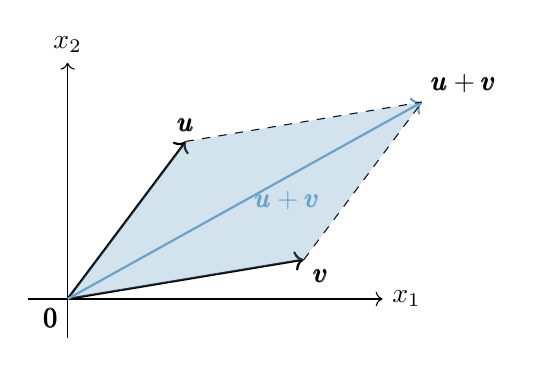
\begin{tikzpicture}
        % Draw axes
        \draw[->] (-0.5, 0) -- (4, 0) node[right] {$x_1$};
        \draw[->] (0, -0.5) -- (0, 3) node[above] {$x_2$};

        % Define the vectors u and v
        \coordinate (O) at (0, 0);
        \coordinate (U) at (1.5, 2);
        \coordinate (V) at (3, 0.5);
        \coordinate (UplusV) at (3+1.5, 2+0.5);

        % Draw vectors
        \draw[->, thick] (O) -- (U);
        \draw[->, thick] (O) -- (V);
        \draw[->, thick, headercolor] (O) -- (UplusV) node[midway, right] {$\vect{u} + \vect{v}$};

        % Draw the parallelogram
        \draw[dashed] (U) -- (UplusV);
        \draw[dashed] (V) -- (UplusV);
        \fill[headercolor, opacity=0.3] (O) -- (U) -- (UplusV) -- (V) -- cycle;

        % Add labels
        \node[above right] at (UplusV) {$\vect{u} + \vect{v}$};
        \node[above] at (U) {$\vect{u}$};
        \node[below right] at (V) {$\vect{v}$};

        % Mark the origin
        \node[below left] at (O) {$\vect{0}$};
    \end{tikzpicture}
    \caption{The parallelogram law of vector addition in $\mathbb{R}^2$.}
    \label{fig:parallelogram-law}
\end{figure}

These ideas generalise to higher-dimensional spaces. More specifically, we can define $\mathbb{R}^n$ as follows.

\begin{definition}
    For each positive integer $n$, we let $\mathbb{R}^n$ denote the collection of ordered $n$-tuples with each entry in $\mathbb{R}$. We often write these elements as $n \times 1$ matrices. We define addition and scalar multiplication of vectors in $\mathbb{R}^n$ in the same way as we do for $\mathbb{R}^2$. That is, we go coordinate-by-coordinate.
\end{definition}

\begin{example}
    If $u_1, u_2, \ldots, u_n \in \mathbb{R}$, then

    \[
    \vect{u} = \left[\begin{array}{c}
    u_1 \\
    u_2 \\
    \vdots \\
    u_n
    \end{array}\right] \in \mathbb{R}^n.
    \]
     
\end{example}

\begin{example}
    If $\vect{u}$ and $\vect{v}$ are in $\mathbb{R}^n$ (with entries denoted $u_1, \ldots, u_n$ and $v_1, \ldots, v_n$, respectively), and $c \in \mathbb{R}$, then

    \[
    \begin{aligned}
    & \vect{u} + \vect{v} = {\left[\begin{array}{c}
    u_1 \\
    u_2 \\
    \vdots \\
    u_n
    \end{array}\right] + \left[\begin{array}{c}
    v_1 \\
    v_2 \\
    \vdots \\
    v_n
    \end{array}\right] = \left[\begin{array}{c}
    u_1 + v_1 \\
    u_2 + v_2 \\
    \vdots \\
    u_n + v_n
    \end{array}\right], \text { and } } 
    & c \vect{u} = c\left[\begin{array}{c}
    u_1 \\
    u_2 \\
    \vdots \\
    u_n
    \end{array}\right] = \left[\begin{array}{c}
    c u_1 \\
    c u_2 \\
    \vdots \\
    c u_n
    \end{array}\right]
    \end{aligned}
    \]   
\end{example}

\begin{custombox}{Algebraic Properties of $\mathbb{R}^n$}
    Let $\vect{u}, \vect{v}, \vect{w} \in \mathbb{R}^n$ and $c, d \in \mathbb{R}$. Then the following properties hold:
    \begin{enumerate}
        \item \textbf{Commutative Property of Addition:} $\vect{u} + \vect{v} = \vect{v} + \vect{u}$.
        \item \textbf{Associative Property of Addition:} $(\vect{u} + \vect{v}) + \vect{w} = \vect{u} + (\vect{v} + \vect{w})$.
        \item \textbf{Additive Identity:} There exists a vector $\vect{0} \in \mathbb{R}^n$ such that $\vect{u} + \vect{0} = \vect{u}$ for all $\vect{u} \in \mathbb{R}^n$.
        \item \textbf{Additive Inverse:} For each $\vect{u} \in \mathbb{R}^n$, there exists a vector $-\vect{u} \in \mathbb{R}^n$ such that $\vect{u} + (-\vect{u}) = \vect{0}$.
        \item \textbf{Distributive Property:} $c(\vect{u} + \vect{v}) = c\vect{u} + c\vect{v}$ and $(c + d)\vect{u} = c\vect{u} + d\vect{u}$.
        \item \textbf{Associative Property of Scalar Multiplication:} $c(d\vect{u}) = (cd)\vect{u}$.
        \item \textbf{Multiplicative Identity:} $1\vect{u} = \vect{u}$.
    \end{enumerate}  
\end{custombox}

A \textbf{linear combination} is a way to combine vectors using scalar multiplication and addition. Given a set of vectors, we multiply each by a scalar and then sum the results. Linear combinations help us understand how vectors relate to each other and whether one vector can be expressed in terms of others.

\begin{definition}{Linear Combinations}
    Given a set of vectors $\vect{v}_1, \vect{v}_2, \ldots, \vect{v}_p \in \mathbb{R}^n$ and scalars $c_1, c_2, \ldots, c_p \in \mathbb{R}$, the vector $\vect{y}$ given by

\[
\vect{y} = c_1 \vect{v}_1 + \cdots + c_p \vect{v}_p
\]

is called a linear combination of $\vect{v}_1, \vect{v}_2, \ldots, \vect{v}_p$ with weights $c_1, c_2, \ldots, c_p$.

\end{definition}

\begin{example}
    Let $\vect{v}_1 = \left[\begin{array}{l}
        1 \\
        2
        \end{array}\right]$ and $\vect{v}_2 = \left[\begin{array}{c}
        1 \\
        -1
        \end{array}\right]$. Some linear combinations of $\vect{v}_1$ and $\vect{v}_2$ include
        
        \[
        \begin{aligned}
        \vect{0} & = 0 \vect{v}_1 + 0 \vect{v}_2 \\
        {\left[\begin{array}{l}
        3 \\
        0
        \end{array}\right] } & = \vect{v}_1 + 2 \vect{v}_2 \\
        {\left[\begin{array}{l}
        -5 \\
        -1
        \end{array}\right] } & = -2 \vect{v}_1 - 3 \vect{v}_2, \text { and } \\
        {\left[\begin{array}{l}
        5 \\
        1
        \end{array}\right] } & = 2 \vect{v}_1 + 3 \vect{v}_2
        \end{aligned}
        \]
        
\end{example}

\subsection*{Vector Equations and Linear Systems}

It is often the case that we wish to know if some vector $\vect{b}$ can be formed as a linear combination of some other set of vectors $\vect{a}_1, \ldots, \vect{a}_n$. The process for figuring this out is given by the following.

\begin{custombox}{Using Matrices to Determine Linear Combinations}
A vector equation

\[
x_1 \vect{a}_1 + x_2 \vect{a}_2 + \cdots + x_n \vect{a}_n = \vect{b}
\]

has the same solution set as the linear system whose augmented matrix is

\[
\left[\begin{array}{lllll}
\vect{a}_1 & \vect{a}_2 & \ldots & \vect{a}_n & \vect{b}
\end{array}\right].
\]    
\end{custombox}

More specifically, if the $\vect{a}_i$'s are in $\mathbb{R}^m$ with

\[
\vect{a}_1 = \left[\begin{array}{c}
a_{11} \\
a_{21} \\
\vdots \\
a_{m1}
\end{array}\right], \quad \vect{a}_2 = \left[\begin{array}{c}
a_{12} \\
a_{22} \\
\vdots \\
a_{m2}
\end{array}\right], \ldots, \quad \vect{a}_n = \left[\begin{array}{c}
a_{1n} \\
a_{2n} \\
\vdots \\
a_{mn}
\end{array}\right], \quad \text{and} \quad \vect{b} = \left[\begin{array}{c}
b_1 \\
b_2 \\
\vdots \\
b_m
\end{array}\right]
\]

then you would row reduce the matrix

\[
\begin{aligned}
& \left[\begin{array}{ccccc}
a_{11} & a_{12} & \ldots & a_{1n} & b_1 \\
a_{21} & a_{22} & \ldots & a_{2n} & b_2 \\
\vdots & \vdots & \ddots & \vdots & \vdots \\
a_{m1} & a_{m2} & \ldots & a_{mn} & b_m
\end{array}\right] \\
& \begin{array}{ccccc}
\hspace{0.5cm} \uparrow & \hspace{0.3cm} \uparrow & \hspace{0.0cm} \ldots & \hspace{0.2cm} \uparrow & \hspace{0.2cm} \uparrow \\
\hspace{0.4cm} \vect{a}_1 & \hspace{0.3cm} \vect{a}_2 & \hspace{0.1cm} \ldots & \hspace{0.2cm} \vect{a}_n & \hspace{0.2cm} \vect{b}
\end{array}
\end{aligned}
\]

to determine if there is some set of weights $x_1, \ldots, x_n$ that work.

\begin{example} Let
\[
\begin{aligned}
&\vect{a}_1=\left[\begin{array}{c}
2 \\
-1 \\
1
\end{array}\right], \quad \vect{a}_2=\left[\begin{array}{c}
0 \\
8 \\
-2
\end{array}\right], \quad \vect{a}_3=\left[\begin{array}{l}
6 \\
5 \\
1
\end{array}\right], \quad \text { and } \vect{b}=\left[\begin{array}{c}
10 \\
3 \\
7
\end{array}\right]
\end{aligned}
\]

We determine if $\vect{b}$ is a linear combination of $\vect{a}_1, \vect{a}_2, \vect{a}_3$, i.e. if there is some set of weights $x_1, x_2, x_3$ such that $x_1 \vect{a}_1 + x_2 \vect{a}_2 + x_3 \vect{a}_3 = \vect{b}$. By the above, we translate this question to the matrix setting.

\[
\begin{alignedat}{3}
& \left[\begin{array}{cccc}
2 & 0 & 6 & 10 \\
-1 & 8 & 5 & 3 \\
1 & -2 & 1 & 7
\end{array}\right]
& \quad & r_1 \leftrightarrow r_3 
& \quad & 
\left[\begin{array}{cccc}
1 & -2 & 1 & 7 \\
-1 & 8 & 5 & 3 \\
2 & 0 & 6 & 10
\end{array}\right] \\[10pt]
& & \quad & \begin{aligned}
    r_2 & \mapsto r_2 + r_1 \\
    r_3 & \mapsto r_3 - 2r_1
\end{aligned}
& \quad & 
\left[\begin{array}{cccc}
1 & -2 & 1 & 7 \\
0 & 6 & 6 & 10 \\
0 & 4 & 4 & -4
\end{array}\right] \\[10pt]
& & \quad & r_3 \mapsto r_3 - \frac{4}{6} r_2
& \quad & 
\left[\begin{array}{cccc}
1 & -2 & 1 & 7 \\
0 & 6 & 6 & 10 \\
0 & 0 & 0 & \blacksquare
\end{array}\right] .
\end{alignedat}
\]

Since the symbol $\blacksquare$ denotes something nonzero, we see that there's no solution, i.e. that $\vect{b}$ is not a linear combination of $\vect{a}_1, \vect{a}_2, \vect{a}_3$.

\end{example}

\begin{example} Let

\[
\vect{a}_1 = \left[\begin{array}{l}
1 \\
0 \\
1
\end{array}\right], \quad
\vect{a}_2 = \left[\begin{array}{c}
-4 \\
6 \\
-4
\end{array}\right], \quad
\vect{a}_3 = \left[\begin{array}{c}
-6 \\
7 \\
5
\end{array}\right], \quad
\text{and } \vect{b} = \left[\begin{array}{c}
11 \\
-5 \\
9
\end{array}\right]
\]

We determine if $\vect{b}$ is a linear combination of $\vect{a}_1, \vect{a}_2, \vect{a}_3$. We reduce the corresponding matrix to echelon form:

\[
\left[\begin{array}{cccc}
1 & -4 & -6 & 11 \\
0 & 6 & 7 & -5 \\
1 & -4 & 5 & 9
\end{array}\right]
\quad r_3 \mapsto r_3 - r_1 \quad
\left[\begin{array}{cccc}
1 & -4 & -6 & 11 \\
0 & 6 & 7 & -5 \\
0 & 0 & 11 & -2
\end{array}\right]
\]

and we see that there is a solution. Now we find what weights $x_1, x_2, x_3$ work by finding the reduced echelon form.

\[
\begin{alignedat}{3}
& r_3 \mapsto \frac{1}{11} r_3 \quad &
& \left[\begin{array}{cccc}
1 & -4 & -6 & 11 \\
0 & 6 & 7 & -5 \\
0 & 0 & 1 & -\frac{2}{11}
\end{array}\right] \\[10pt]
& \begin{aligned}
    r_2 & \mapsto r_2 - 7r_3 \\
    r_1 & \mapsto r_1 + 6r_3
\end{aligned} & \quad &
\left[\begin{array}{cccc}
1 & -4 & 0 & \frac{109}{11} \\
0 & 6 & 0 & -\frac{41}{11} \\
0 & 0 & 1 & -\frac{2}{11}
\end{array}\right]
\end{alignedat}
\]

\[
\begin{alignedat}{3}
& r_2 \mapsto \frac{1}{6}r_2 \quad &
& \left[\begin{array}{cccc}
1 & -4 & 0 & \frac{109}{11} \\
0 & 1 & 0 & -\frac{41}{66} \\
0 & 0 & 1 & -\frac{2}{11}
\end{array}\right] \\[10pt]
& r_1 \mapsto r_1 + 4r_2 \quad &
& \left[\begin{array}{cccc}
1 & 0 & 0 & \frac{245}{38} \\
0 & 1 & 0 & -\frac{41}{66} \\
0 & 0 & 1 & -\frac{2}{11}
\end{array}\right],
\end{alignedat}
\]

so $\left(x_1, x_2, x_3\right)=\left(\frac{245}{33},-\frac{41}{66},-\frac{2}{11}\right)$. Since there are no free variables, this is the unique solution.

\end{example}

The \textbf{span} of a set of vectors is the collection of all possible linear combinations of those vectors. In other words, it's the set of all vectors you can reach by scaling and adding the given vectors. The span gives us insight into the "space" those vectors cover:

\begin{definition}{Span of a Set of Vectors}
    If $\vect{v}_1, \ldots, \vect{v}_p$ are in $\mathbb{R}^n$, then the set of all linear combinations of $\vect{v}_1, \ldots, \vect{v}_p$ is denoted by \text{Span} $\left\{\vect{v}_1, \ldots, \vect{v}_p\right\}$ and is called the subset of $\mathbb{R}^n$ spanned by $\vect{v}_1, \ldots, \vect{v}_p$. In other words, the span of $\vect{v}_1, \ldots, \vect{v}_p$ is all vectors that can be written in the form
    $$
    c_1 \vect{v}_1 + \cdots + c_p \vect{v}_p
    $$
    with $c_1, \ldots, c_p$ scalars.

\end{definition}

\section{Matrix Equations}
In the previous sections, we explored different ways of representing linear relationships. For instance, we looked at individual linear equations, such as  
\[
2x_1 + 3x_2 = 5,
\]
and systems of linear equations, like  
\[
\begin{aligned}
x_1 + 2x_2 &= 4 \\
3x_1 - x_2 &= 2.
\end{aligned}
\]
We also expressed these systems as vector equations, such as  
\[
x_1 \begin{bmatrix} 1 \\ 3 \end{bmatrix} + x_2 \begin{bmatrix} 2 \\ -1 \end{bmatrix} = \begin{bmatrix} 4 \\ 2 \end{bmatrix}.
\]

Now, it's time to introduce a powerful new form: the \textbf{matrix equation}. This compact representation allows us to handle systems of linear equations efficiently using matrix notation. In this form, our system becomes  
\[
A \vect{x} = \vect{b},
\]
where \(A\) is a matrix, \(\vect{x}\) is a vector of variables, and \(\vect{b}\) is the result vector. Matrix equations give us a structured, algebraic approach to solving systems.

\begin{definition}{Matrix Equation}
  If $A$ is an $m \times n$ matrix with columns $\vect{a}_1, \ldots, \vect{a}_n$, and if $\vect{x} \in \mathbb{R}^n$, then the product of $A$ and $\vect{x}$, denoted by $A \vect{x}$, is

\[
A \vect{x} = \left[\begin{array}{llll}
\vect{a}_1 & \vect{a}_2 & \ldots & \vect{a}_n
\end{array}\right] \left[\begin{array}{c}
x_1 \\
x_2 \\
\vdots \\
x_n
\end{array}\right] = x_1 \vect{a}_1 + x_2 \vect{a}_2 + \cdots + x_n \vect{a}_n
\]
    
\end{definition}

\begin{example}
    \[
\begin{aligned}
{\left[\begin{array}{lll}
4 & 1 & 2 \\
8 & 0 & 3
\end{array}\right]\left[\begin{array}{l}
2 \\
1 \\
4
\end{array}\right] } & =2\left[\begin{array}{l}
4 \\
8
\end{array}\right]+1\left[\begin{array}{l}
1 \\
0
\end{array}\right]+4\left[\begin{array}{l}
2 \\
3
\end{array}\right] \\
& =\left[\begin{array}{c}
8 \\
16
\end{array}\right]+\left[\begin{array}{l}
1 \\
0
\end{array}\right]+\left[\begin{array}{c}
8 \\
12
\end{array}\right] \\
& =\left[\begin{array}{l}
17 \\
28
\end{array}\right]
\end{aligned}
\]
\end{example}

Building a bit on the main result from the preceding section, we have the following theorem.

\newpage

\begin{theorem}
    If $A$ is an $m \times n$ matrix, with columns $\vect{a}_1, \ldots, \vect{a}_n \in \mathbb{R}^m$ and if $\vect{b} \in \mathbb{R}^m$, the matrix equation

\[
A \vect{x} = \vect{b}
\]

has the same solution set as the vector equation

\[
x_1 \vect{a}_1 + x_2 \vect{a}_2 + \cdots + x_n \vect{a}_n = \vect{b}
\]

which, in turn, has the same solution set as the system of linear equations with augmented matrix

\[
\left[\begin{array}{lllll}
\vect{a}_1 & \vect{a}_2 & \ldots & \vect{a}_n & \vect{b}
\end{array}\right].
\]

\end{theorem}

This theorem is essential because it ties together the three forms of representing and solving systems of linear equations: matrix equations, vector equations, and systems of equations with augmented matrices. It shows that no matter which form we use, they all lead to the same solution set.

By stating that the matrix equation \( A \vect{x} = \vect{b} \) is equivalent to the vector equation \( x_1 \vect{a}_1 + x_2 \vect{a}_2 + \cdots + x_n \vect{a}_n = \vect{b} \), we can interpret solving a matrix equation as finding the right combination of the columns of \( A \) that yields \( \vect{b} \). This connection allows us to visualize the problem in terms of vector spaces and linear combinations.

Moreover, the theorem shows that this same process is reflected in the augmented matrix, where row reduction reveals the solution through elementary row operations. So whether we approach the problem algebraically, geometrically, or algorithmically, we are dealing with the same underlying structure. This unifying perspective simplifies our approach to solving systems and provides flexibility in how we choose to represent and manipulate the problem.

\begin{remark}
    The equation $A \vect{x} = \vect{b}$ has a solution if and only if $\vect{b}$ is a linear combination of the columns of $A$.
\end{remark}

The following theorem tells us when the column vectors of an $m \times n$ matrix (the columns are vectors in $\mathbb{R}^m$, since there are $m$ rows) can be used to generate all of $\mathbb{R}^m$. This basically summarises several things we have already seen in different contexts.

\begin{theorem}
Let \( A \) be an \( m \times n \) matrix. Then the following statements are equivalent:
\begin{enumerate}[label=(\alph*)]
    \item For each \( \vect{b} \in \mathbb{R}^m \), the equation \( A \vect{x} = \vect{b} \) has a solution.
    \item Each \( \vect{b} \in \mathbb{R}^m \) is a linear combination of the columns of \( A \).
    \item The columns of \( A \) span \( \mathbb{R}^m \).
    \item The matrix \( A \) has a pivot position in every row.
\end{enumerate}
\end{theorem}

This theorem shows that several seemingly different ideas are in fact equivalent. The existence of a solution to the matrix equation \( A \vect{x} = \vect{b} \) (statement (a)) depends on whether the columns of \( A \) can form any vector in \( \mathbb{R}^m \) (statement (b)). Geometrically, this means the columns span the entire space \( \mathbb{R}^m \) (statement (c)).

Finally, the presence of a pivot position in every row (statement (d)) gives an algebraic condition that guarantees the span of the columns covers \( \mathbb{R}^m \), ensuring that there is always a solution to \( A \vect{x} = \vect{b} \).

This equivalence is a powerful tool, as it connects solutions, linear combinations, and geometric interpretations, while also providing a concrete method (checking for pivot positions) to verify these properties.

\begin{custombox}{Row-Vector Rule for Computing \( A \vect{x} \)}
Assuming the product \( A \vect{x} \) is defined, the \( i \)-th entry in \( A \vect{x} \) is the sum of the products of corresponding entries from row \( i \) of \( A \) and the vector \( \vect{x} \). In other words, the \( i \)-th entry of \( A \vect{x} \) is the dot product of the vector forming the \( i \)-th row of \( A \) and the vector \( \vect{x} \).
    
\end{custombox}


This rule simplifies the matrix multiplication process by breaking it down into smaller, familiar operations — dot products — making it easier to compute and understand. It also highlights the connection between matrix multiplication and linear combinations, as the product \( A \vect{x} \) is a linear combination of the rows of \( A \) with weights given by the entries of \( \vect{x} \).

\begin{example} Let

\[
A=\left[\begin{array}{ccc}
1 & -1 & 4 \\
5 & 0 & 2
\end{array}\right], \text { and } \vect{x}=\left[\begin{array}{l}
2 \\
1 \\
5
\end{array}\right]
\]

Then

\[
\begin{aligned}
{\left[\begin{array}{ccc}
1 & -1 & 4 \\
5 & 0 & 2
\end{array}\right]\left[\begin{array}{l}
2 \\
1 \\
5
\end{array}\right] } & =\left[\begin{array}{c}
1 \cdot 2+(-1) \cdot 1+4 \cdot 5 \\
5 \cdot 2+0 \cdot 1+2 \cdot 5
\end{array}\right] \\
& =\left[\begin{array}{c}
21 \\
20
\end{array}\right]
\end{aligned}
\]
\end{example}

Notice that the number of columns in $A$ must match the number of rows in $\vect{x}$, for otherwise the dot product would not make sense!

The next theorem captures two important properties of matrix-vector multiplication: \textbf{distributivity} and \textbf{scalar multiplication}. These properties mirror the familiar rules of algebra but now apply in the context of matrices and vectors.

\begin{theorem}
If \( A \) is an \( m \times n \) matrix, \( \vect{u} \) and \( \vect{v} \) are vectors in \( \mathbb{R}^n \), and \( c \) is a scalar, then:

\begin{enumerate}[label=(\alph*)]
    \item \( A(\vect{u} + \vect{v}) = A \vect{u} + A \vect{v} \)  


    \item \( A(c \vect{u}) = c(A \vect{u}) \)  

\end{enumerate}
\end{theorem}

Property (a) shows that matrix multiplication distributes over vector addition. It means that multiplying \( A \) by the sum of two vectors is the same as multiplying \( A \) by each vector separately and then adding the results.     Property (b) illustrates that scalar multiplication commutes with matrix multiplication. Multiplying a vector by a scalar first, then applying the matrix, gives the same result as applying the matrix first and then multiplying the resulting vector by the scalar.

\begin{example} Let

\[
A = \left[\begin{array}{cccc}
1 & 5 & -2 & 0 \\
-3 & 1 & 9 & -5 \\
4 & -8 & -1 & 7
\end{array}\right], \quad \vect{p} = \left[\begin{array}{c}
3 \\
-2 \\
0 \\
-4
\end{array}\right], \quad \vect{b} = \left[\begin{array}{c}
-7 \\
9 \\
0
\end{array}\right]
\]

It can be shown that $\vect{p}$ is a solution of $A \vect{x} = \vect{b}$. Use this fact to write $\vect{b}$ as a linear combination of the columns of $A$.
    
\end{example}  

\begin{solution} Since $\vect{p}$ is a solution to $A \vect{x} = \vect{b}$, we have:
    \[
    A \vect{p} = \vect{b}.
    \]
    
    We can express $\vect{b}$ as a linear combination of the columns of $A$ using the entries of $\vect{p}$. Let $\vect{a}_1$, $\vect{a}_2$, $\vect{a}_3$, and $\vect{a}_4$ denote the columns of $A$, so:
    \[
    A = \left[ \vect{a}_1 \ \big| \ \vect{a}_2 \ \big| \ \vect{a}_3 \ \big| \ \vect{a}_4 \right].
    \]
    
    Thus,
    \[
    \vect{b} = p_1 \vect{a}_1 + p_2 \vect{a}_2 + p_3 \vect{a}_3 + p_4 \vect{a}_4.
    \]
    
    Now, we compute each term one at a time.
    
    \textbf{Compute $p_1 \vect{a}_1$:}
    \[
    p_1 \vect{a}_1 = 3 \left[\begin{array}{c}
    1 \\
    -3 \\
    4
    \end{array}\right] = \left[\begin{array}{c}
    3 \\
    -9 \\
    12
    \end{array}\right].
    \]
    
    \textbf{Compute $p_2 \vect{a}_2$:}
    \[
    p_2 \vect{a}_2 = (-2) \left[\begin{array}{c}
    5 \\
    1 \\
    -8
    \end{array}\right] = \left[\begin{array}{c}
    -10 \\
    -2 \\
    16
    \end{array}\right].
    \]
    
    \textbf{Compute $p_3 \vect{a}_3$:}
    \[
    p_3 \vect{a}_3 = 0 \left[\begin{array}{c}
    -2 \\
    9 \\
    -1
    \end{array}\right] = \left[\begin{array}{c}
    0 \\
    0 \\
    0
    \end{array}\right].
    \]
    
    \textbf{Compute $p_4 \vect{a}_4$:}
    \[
    p_4 \vect{a}_4 = (-4) \left[\begin{array}{c}
    0 \\
    -5 \\
    7
    \end{array}\right] = \left[\begin{array}{c}
    0 \\
    20 \\
    -28
    \end{array}\right].
    \]
    
    \textbf{Add the computed vectors to find $\vect{b}$:}
    \[
    \vect{b} = p_1 \vect{a}_1 + p_2 \vect{a}_2 + p_3 \vect{a}_3 + p_4 \vect{a}_4 = \left[\begin{array}{c}
    3 \\
    -9 \\
    12
    \end{array}\right] + \left[\begin{array}{c}
    -10 \\
    -2 \\
    16
    \end{array}\right] + \left[\begin{array}{c}
    0 \\
    0 \\
    0
    \end{array}\right] + \left[\begin{array}{c}
    0 \\
    20 \\
    -28
    \end{array}\right].
    \]
    
    Now, compute the sum step by step.
    
    \textbf{Step 1: Add $p_1 \vect{a}_1$ and $p_2 \vect{a}_2$:}
    \[
    \left[\begin{array}{c}
    3 \\
    -9 \\
    12
    \end{array}\right] + \left[\begin{array}{c}
    -10 \\
    -2 \\
    16
    \end{array}\right] = \left[\begin{array}{c}
    -7 \\
    -11 \\
    28
    \end{array}\right].
    \]
    
    \textbf{Step 2: Add $p_3 \vect{a}_3$ (which is zero) to the result:}
    \[
    \left[\begin{array}{c}
    -7 \\
    -11 \\
    28
    \end{array}\right] + \left[\begin{array}{c}
    0 \\
    0 \\
    0
    \end{array}\right] = \left[\begin{array}{c}
    -7 \\
    -11 \\
    28
    \end{array}\right].
    \]
    
    \textbf{Step 3: Add $p_4 \vect{a}_4$ to the result:}
    \[
    \left[\begin{array}{c}
    -7 \\
    -11 \\
    28
    \end{array}\right] + \left[\begin{array}{c}
    0 \\
    20 \\
    -28
    \end{array}\right] = \left[\begin{array}{c}
    -7 \\
    9 \\
    0
    \end{array}\right].
    \]
    
    \textbf{Final Result:}
    \[
    \vect{b} = \left[\begin{array}{c}
    -7 \\
    9 \\
    0
    \end{array}\right].
    \]
    
    \textbf{Conclusion:}
    
    We have expressed $\vect{b}$ as a linear combination of the columns of $A$ using the entries of $\vect{p}$:
    \[
    \vect{b} = 3 \vect{a}_1 - 2 \vect{a}_2 + 0 \vect{a}_3 - 4 \vect{a}_4.
    \]
\end{solution}

\section{Solution Sets of Linear Systems}
Solution sets of linear systems play a crucial role in the study of linear algebra and will reappear in various contexts throughout the subject. In this section, we use vector notation to provide clear, explicit, and geometric descriptions of these solution sets.

A linear system is said to be \textit{homogeneous} if it can be written in the form

\[
A \vect{x} = \vect{0}
\]

where $A$ is an $m \times n$ matrix and $\vect{0}$ is the zero vector in $\mathbb{R}^m$. Such a system always has the \textit{trivial solution}, namely $\vect{x} = \vect{0}$ (the zero vector in $\mathbb{R}^n$, not $\mathbb{R}^m$).

Since homogeneous systems always have the trivial solution, the interesting question is whether or not they have \textit{nontrivial solutions}.

\begin{remark}
    The homogeneous equation $A \vect{x} = \vect{0}$ has a nontrivial solution if and only if the equation has at least one free variable.
\end{remark}

\begin{example}
    Determine if the following homogeneous system has a nontrivial solution. If it does, describe the solution set using the free variable(s).
\[
\begin{aligned}
2 x_1+x_2-3 x_3 & =0 \\
x_1-x_2+x_3 & =0 \\
-2 x_1+5 x_2-7 x_3 & =0
\end{aligned}
\]

\end{example}

\begin{solution}
    We let $A$ be the coefficient matrix of the system, and reduce the augmented mat rix [ $\left.\begin{array}{cc}A & 0\end{array}\right]$ to echelon form (notice how we put the second equation first in order to simplify the computation a bit):

\[
\begin{aligned}
{\left[\begin{array}{cccc}
1 & -1 & 1 & 0 \\
2 & 1 & -3 & 0 \\
-2 & 5 & -7 & 0
\end{array}\right] } & \sim\left[\begin{array}{cccc}
1 & -1 & 1 & 0 \\
0 & 3 & -5 & 0 \\
0 & 3 & -5 & 0
\end{array}\right] \\
& \sim\left[\begin{array}{cccc}
1 & -1 & 1 & 0 \\
0 & 3 & -5 & 0 \\
0 & 0 & 0 & 0
\end{array}\right]
\end{aligned}
\]

so we see that $x_3$ is a free variable, and as a result we have nontrivial solutions. Now we get the reduced echelon form:

\[
\begin{aligned}
{\left[\begin{array}{cccc}
1 & -1 & 1 & 0 \\
0 & 3 & -5 & 0 \\
0 & 0 & 0 & 0
\end{array}\right] } & \sim\left[\begin{array}{cccc}
1 & -1 & 1 & 0 \\
0 & 1 & -\frac{5}{3} & 0 \\
0 & 0 & 0 & 0
\end{array}\right] \\
& \sim\left[\begin{array}{cccc}
1 & 0 & -\frac{2}{3} & 0 \\
0 & 1 & -\frac{5}{3} & 0 \\
0 & 0 & 0 & 0
\end{array}\right]
\end{aligned}
\]

This gives us the equations

\[
\begin{aligned}
& x_1-\frac{2}{3} x_3=0 \quad \Longrightarrow x_1=\frac{2}{3} x_3 \\
& x_2-\frac{5}{3} x_3=0 \quad \Longrightarrow x_2=\frac{5}{3} x_3
\end{aligned}
\]


In vector form, the solution $\vect{x}$ of the equation $A \vect{x}=0$ is written

\[
\vect{x}=\left[\begin{array}{l}
x_1 \\
x_2 \\
x_3
\end{array}\right]=\left[\begin{array}{c}
\frac{2}{3} x_3 \\
\frac{5}{3} x_3 \\
x_3
\end{array}\right]=x_3\left[\begin{array}{c}
\frac{2}{3} \\
\frac{5}{3} \\
1
\end{array}\right]
\]


Since $x_3$ can be anything, in geometric terms this solution set describes the line in $\mathbb{R}^3$ extending from the origin through the point $\left(\frac{2}{3}, \frac{5}{3}, 1\right)$.
\end{solution}


\begin{custombox}{Parametric Vector Form}
    Whenever a solution set is described explicitly with vectors (as in the preceding example), we say that the solution is in \textbf{parametric vector form}.
\end{custombox}

\begin{example} Describe all solutions of the homogeneous equation


\[
    x_1-2 x_2-5 x_3=0
\]

\end{example}

\begin{solution}

Writing this system in a matrix, we would see that $x_2$ and $x_3$ are free variables, and $x_1$ is a basic variable with $x_1=2 x_2+5 x_3$. Hence the general solution is

$$
\vect{x}=\left[\begin{array}{l}
x_1 \\
x_2 \\
x_3
\end{array}\right]=\left[\begin{array}{c}
2 x_2+5 x_3 \\
x_2 \\
x_3
\end{array}\right]=x_2\left[\begin{array}{l}
2 \\
1 \\
0
\end{array}\right]+x_3\left[\begin{array}{l}
5 \\
0 \\
1
\end{array}\right]
$$

where the right-most part of this equation is the \textbf{parametric vector} form of the solution set. In this case, the entire solution set is a plane in $\mathbb{R}^3$ that contains the two lines extending from $(0,0,0)$ to $(2,1,0)$, and from $(0,0,0)$ to $(5,0,1)$.
\end{solution}

When a \textit{nonhomogeneous} linear system has many solutions, the general solution can be written in parametric vector form as one vector plus arbitrary linear combinations of vectors that satisfy the corresponding homogeneous system.

\begin{example} We reconsider the homogeneous system at the beginning of this section, except this time it will be nonhomogeneous (i.e., the right side will not be all zeroes):

\[
\begin{aligned}
2 x_1 + x_2 - 3 x_3 & = 2 \\
x_1 - x_2 + x_3 & = 1 \\
-2 x_1 + 5 x_2 - 7 x_3 & = -2
\end{aligned}
\]

As before, we perform row operations on the augmented matrix \(\left[\begin{array}{cc} A & \vect{b} \end{array}\right]\) where \( A \) is the same coefficient matrix and

\[
\vect{b} = \begin{bmatrix}
2 \\
1 \\
-2
\end{bmatrix}
\]

and we find that

\[
\left[\begin{array}{cccc}
1 & -1 & 1 & 1 \\
2 & 1 & -3 & 2 \\
-2 & 5 & -7 & -2
\end{array}\right]
\sim
\left[\begin{array}{cccc}
1 & 0 & -\frac{2}{3} & 1 \\
0 & 1 & -\frac{5}{3} & 0 \\
0 & 0 & 0 & 0
\end{array}\right]
\]

Hence,

\[
\begin{aligned}
x_1 &= 1 + \frac{2}{3} x_3, \text{ and } \\
x_2 &= \frac{5}{3} x_3
\end{aligned}
\]

This can be written as

\[
\vect{x} = \begin{bmatrix}
x_1 \\
x_2 \\
x_3
\end{bmatrix} =
\begin{bmatrix}
1 + \frac{2}{3} x_3 \\
\frac{5}{3} x_3 \\
x_3
\end{bmatrix}
= \begin{bmatrix}
1 \\
0 \\
0
\end{bmatrix} + x_3 \begin{bmatrix}
\frac{2}{3} \\
\frac{5}{3} \\
1
\end{bmatrix}
\]

which has the form we claimed. This is the equation of the line through the point \((1,0,0)\) that is parallel to the line extending from \((0,0,0)\) through \(\left(\frac{2}{3}, \frac{5}{3}, 1\right)\).

\end{example}

We summarise the general situation with the following theorem. It might be best to think of the conclusion as shifting all homogeneous solutions by the vector $\vect{p}$.

\begin{theorem}
    Suppose $A \vect{x} = \vect{b}$ is consistent for some $\vect{b}$, and let $\vect{p}$ be a solution. Then the solution set of $A \vect{x} = \vect{b}$ is the set of all vectors of the form
    \[
    \vect{w} = \vect{p} + \vect{v}_h,
    \]
    where $\vect{v}_h$ is any solution of the homogeneous equation $A \vect{x} = \vect{0}$.
\end{theorem}

\begin{example} Write the general solution of

\[
x_1-2 x_2-5 x_3=3
\]

in parametric vector form. In geometric terms, what does this solution set look like in comparison to the solution set of the equation $x_1-2 x_2-5 x_3=0$ that we saw earlier?
\end{example}

\begin{solution}
        Let us solve the equation:
        \[
        x_1 - 2 x_2 - 5 x_3 = 3
        \]
        
        To express the general solution, we solve for \( x_1 \) in terms of \( x_2 \) and \( x_3 \):
    
        \[
        \begin{aligned}
        x_1 &= 3 + 2x_2 + 5x_3, \\
        x_2 &= x_2, \\
        x_3 &= x_3.
        \end{aligned}
        \]
        
        We can express the solution set in \textit{parametric vector form}:
        \[
        \begin{bmatrix}
        x_1 \\
        x_2 \\
        x_3
        \end{bmatrix}
        =
        \begin{bmatrix}
        3 \\
        0 \\
        0
        \end{bmatrix}
        +
        x_2
        \begin{bmatrix}
        2 \\
        1 \\
        0
        \end{bmatrix}
        +
        x_3
        \begin{bmatrix}
        5 \\
        0 \\
        1
        \end{bmatrix}, \quad \text{for all } s, t \in \mathbb{R}.
        \]
        
        \textbf{Geometric Interpretation:} The solution set represents a plane in \(\mathbb{R}^3\). This plane is parallel to the plane defined by the homogeneous equation:
        \[
        x_1 - 2 x_2 - 5 x_3 = 0
        \]
        
        The homogeneous solution set can be expressed as:
        \[
        \begin{bmatrix}
        x_1 \\
        x_2 \\
        x_3
        \end{bmatrix}
        =
        x_2
        \begin{bmatrix}
        2 \\
        1 \\
        0
        \end{bmatrix}
        +
        x_3
        \begin{bmatrix}
        5 \\
        0 \\
        1
        \end{bmatrix}, \quad \text{for all } s, t \in \mathbb{R}.
        \]
        
        Comparing both solution sets, we observe that the original solution is the homogeneous solution shifted by the vector \(\begin{bmatrix} 3 \\ 0 \\ 0 \end{bmatrix}\). Geometrically, this means the plane defined by \( x_1 - 2 x_2 - 5 x_3 = 3 \) is parallel to, but not the same as, the plane defined by \( x_1 - 2 x_2 - 5 x_3 = 0 \). The two planes are offset along the \( x_1 \)-axis by 3 units. The general solution of the equation \( x_1 - 2 x_2 - 5 x_3 = 3 \) is a plane in \(\mathbb{R}^3\) that is parallel to the solution set of the homogeneous equation \( x_1 - 2 x_2 - 5 x_3 = 0 \), but shifted away from the origin. \end{solution}

        \begin{example} Find the parametric equation of the line through $\vect{a}=\left[\begin{array}{c}3 \\ -2\end{array}\right]$ that is also parallel to $\vect{b}=\left[\begin{array}{c}-7 \\ 6\end{array}\right]$.
        \end{example}

        \begin{solution}
            The line through $\vect{a}$ parallel to $\vect{b}$ is given by the equation $\vect{r}=\vect{a}+t \vect{b}$, where $t$ is a parameter. Substituting the given vectors, we have
            \[
            \begin{aligned}
            \vect{r} &=\left[\begin{array}{c}
            3 \\
            -2
            \end{array}\right]+t\left[\begin{array}{c}
            -7 \\
            6
            \end{array}\right] \\
            &=\left[\begin{array}{c}
            3-7 t \\
            -2+6 t
            \end{array}\right]
            \end{aligned}
            \]
            This is the parametric equation of the line through $\vect{a}$ that is parallel to $\vect{b}$.
        \end{solution}

\section{Linear Independence}
We conclude this section by introducing one of the most important concepts in linear algebra: \textit{linear independence}. This concept is fundamental to understanding the structure of vectors and their relationships in vector spaces.

\begin{definition}
    An indexed set of vectors $\left\{\vect{v}_1, \ldots, \vect{v}_p\right\} \subset \mathbb{R}^n$ is said to be \textbf{linearly independent} if the vector equation
    
    \[
    x_1 \vect{v}_1 + \cdots + x_p \vect{v}_p = \vect{0}
    \]
    
    has only the trivial solution, i.e., if the only solution is $\left(x_1, \ldots, x_p\right) = (0, \ldots, 0)$. Likewise, the set $\left\{\vect{v}_1, \ldots, \vect{v}_p\right\}$ is said to be \textbf{linearly dependent} if there exist weights $c_1, \ldots, c_p$, not all zero, such that
    
    \[
    c_1 \vect{v}_1 + \cdots + c_p \vect{v}_p = \vect{0}
    \]
    
    We call such an equation a \textit{linear dependence relation} when the weights are not all zero.
    \end{definition}
    
    \begin{remark}
        A set of vectors cannot be both linearly independent and linearly dependent, but it must be one of them!
    \end{remark}

    Determining if a set of vectors is linearly independent is tantamount to solving the matrix equation

    \[
    A \vect{x}=0,
    \]

where the columns of $A$ are given by the vectors. The set of vectors is linearly independent if and only if the only solution is $\vect{x}=\vect{0}$. Otherwise, there is some linear dependence relation.

    \begin{example}
        Determine if the following vectors in $\mathbb{R}^3$ are linearly independent:

        \[
        \vect{v}_1 = \left[\begin{array}{l}
        2 \\
        1 \\
        2
        \end{array}\right], \quad \vect{v}_2 = \left[\begin{array}{l}
        1 \\
        1 \\
        1
        \end{array}\right], \quad \vect{v}_3 = \left[\begin{array}{l}
        0 \\
        1 \\
        1
        \end{array}\right]
        \]
    \end{example}

    \begin{solution}
        We begin by reducing the corresponding augmented matrix to echelon form:

\[
\begin{aligned}
{\left[\begin{array}{llll}
2 & 1 & 0 & 0 \\
1 & 1 & 1 & 0 \\
2 & 1 & 1 & 0
\end{array}\right] } & \sim\left[\begin{array}{llll}
1 & 1 & 1 & 0 \\
2 & 1 & 0 & 0 \\
2 & 1 & 1 & 0
\end{array}\right] \\
& \sim\left[\begin{array}{cccc}
1 & 1 & 1 & 0 \\
0 & -1 & -2 & 0 \\
0 & -1 & -1 & 0
\end{array}\right] \\
& \sim\left[\begin{array}{cccc}
1 & 1 & 1 & 0 \\
0 & -1 & -2 & 0 \\
0 & 0 & 1 & 0
\end{array}\right]
\end{aligned}
\]

from which we see that there is a solution. Now we want to know if the solution is the trivial solution $(0,0,0)$. Normally, we would continue row operations until we reach reduced echelon form, but we can be smarter about this. Notice first of all that there are no bad rows (so there is at least one solution), which we expect since a homogeneous system always has at least the trivial solution. Since there are no free variables, we see there is exactly one solution. This tells us that the solution must be

\[
\vect{x}=\left[\begin{array}{l}
x_1 \\
x_2 \\
x_3
\end{array}\right]=\left[\begin{array}{l}
0 \\
0 \\
0
\end{array}\right]
\]

Hence the set of vectors $\left\{\vect{v}_1, \vect{v}_2, \vect{v}_3\right\}$ is linearly independent.
\end{solution}

In general, it is very useful to determine if some set of vectors is linearly independent, so it is good to have
some theorems to handle this problem quickly in certain special cases.

\begin{theorem}
    \begin{enumerate}[(a)]
        \item If a set of vectors contains the zero vector, then the set is linearly dependent.
        \item If a set of vectors contains a scalar multiple of another vector, then the set is linearly dependent.
        \item If a set of vectors contains more vectors than there are entries in each vector, then the set is linearly dependent.
    \end{enumerate}
\end{theorem}

The last part of the theorem is particularly useful, as it allows us to quickly determine if a set of vectors is linearly dependent by checking if one of the vectors is a linear combination of the others. We can formalise this idea in the following corollary.

\begin{corollary}
    An indexed set $S = \left\{\vect{v}_1, \ldots, \vect{v}_p\right\}$ of two or more vectors is linearly dependent if and only if at least one of the vectors in $S$ is a linear combination of the others. If $S$ is linearly dependent and $\vect{v}_1 \neq \vect{0}$, then some $\vect{v}_j$ (with $1 < j \leq p$) is a linear combination of the preceding vectors $\vect{v}_1, \ldots, \vect{v}_{j-1}$.
\end{corollary}

\begin{remark}
    The corollary tells us that if a set of vectors is linearly dependent, then at least one of the vectors is redundant, as it can be expressed as a linear combination of the others. This redundancy is what causes the linear dependence. This does not mean that every vector in $S$ is a linear combination of the others, but only that \textit{at least one} vector in a linearly dependent set is a linear combination of others.
\end{remark}

\begin{example} Let
    \[
    \vect{u} = \left[\begin{array}{l}
    2 \\
    1 \\
    1
    \end{array}\right], \quad \vect{v} = \left[\begin{array}{l}
    4 \\
    3 \\
    5
    \end{array}\right], \quad \vect{w} = \left[\begin{array}{l}
    1 \\
    1 \\
    1
    \end{array}\right], \quad \vect{z} = \left[\begin{array}{l}
    0 \\
    0 \\
    1
    \end{array}\right].
    \]

    \begin{enumerate}[(a)]
        \item Is any pair of these vectors (e.g. $\{\vect{u}, \vect{v}\}$) linearly dependent? Explain.
        \item Does the answer to part (a) tell us that $\{\vect{u}, \vect{v}, \vect{w}, \vect{z}\}$ is linearly independent?
        \item Is $\{\vect{u}, \vect{v}, \vect{w}, \vect{z}\}$ linearly dependent? You should be able to answer this question without any computation.
    \end{enumerate}
\end{example}

\begin{solution}
    \begin{enumerate}[(a)]
        \item 
        To determine if any pair of these vectors is linearly dependent, we check whether one vector is a scalar multiple of the other.

        \textbf{Checking the pair $\{\vect{u}, \vect{v}\}$:} Assume there exists a scalar $k$ such that:
    
        \[
        \vect{v} = k \vect{u}.
        \]
        
        Compute $k$ using the first component:
        \[
        k = \dfrac{v_1}{u_1} = \dfrac{4}{2} = 2.
        \]
        
        Verify with the second component:
        \[
        v_2 = k u_2 \implies 3 = 2 \times 1 \implies 3 = 2.
        \]
        
        Since $3 \ne 2$, $\vect{v}$ is not a scalar multiple of $\vect{u}$.
        
        \textbf{Checking the pair $\{\vect{u}, \vect{w}\}$:} Assume there exists a scalar $k$ such that:
        \[
        \vect{u} = k \vect{w}.
        \]
        
        Compute $k$ using the first component:
        \[
        k = \dfrac{u_1}{w_1} = \dfrac{2}{1} = 2.
        \]
        
        Verify with the second component:
        \[
        u_2 = k w_2 \implies 1 = 2 \times 1 \implies 1 = 2.
        \]
        
        Since $1 \ne 2$, $\vect{u}$ is not a scalar multiple of $\vect{w}$.
        
        \textbf{Checking the pair $\{\vect{w}, \vect{z}\}$:} Since $z_1 = 0$ and $w_1 = 1$, assuming $\vect{w} = k \vect{z}$ leads to:
        \[
        w_1 = k z_1 \implies 1 = k \times 0 \implies 1 = 0,
        \] which is a contradiction.
    
        \item No, the fact that no pair is linearly dependent does not imply that the entire set is linearly independent. Linear independence requires that the only solution to:
        \[
        c_1 \vect{u} + c_2 \vect{v} + c_3 \vect{w} + c_4 \vect{z} = \vect{0}
        \]
        is $c_1 = c_2 = c_3 = c_4 = 0$.
        
        \item Yes, the set is linearly dependent. In $\mathbb{R}^3$, any set of more than three vectors must be linearly dependent because the maximum number of linearly independent vectors in $\mathbb{R}^3$ is three.
    \end{enumerate}
        
        \textbf{Conclusion:}
        
        \begin{enumerate}[(a)]
            \item No pair of these vectors is linearly dependent.
            \item The answer to part (a) does not guarantee that the entire set is linearly independent.
            \item The set $\{\vect{u}, \vect{v}, \vect{w}, \vect{z}\}$ is linearly dependent without the need for further computation.
        \end{enumerate}

\end{solution}


\chapter{Matrix Algebra}\label{chap:ch9}

In the previous chapters, we explored concepts like linear equations, echelon forms, row reductions, linear independence, vector equations, and matrix equations. Now, to take our problem-solving skills to the next level, we need to dive into matrix algebra. Matrix operations allow us to handle complex systems more efficiently, building on the foundations we've established. The tools and techniques in this chapter will streamline the way we work with multiple matrices and lead us toward deeper insights, including key ideas like the Invertible Matrix Theorem.

\section{Matrix Arithmetic}
Matrix arithmetic like adding, subtracting, scaling, and multiplying let you combine and manipulate matrices in simple ways. These operations are the building blocks for more complex matrix manipulations, like solving systems of equations and finding inverses.


\subsection*{Addition and Scalar Multiplication}
We begin with the definition of matrix addition.

\begin{definition}{Matrix Addition}
    Let $A$ and $B$ be $m \times n$ matrices. The \textbf{sum} of $A$ and $B$, denoted $A + B$, is the $m \times n$ matrix whose entries are obtained by adding the corresponding entries of $A$ and $B$.

    Given matrices

    $$
    A=\left[\begin{array}{cccc}
    a_{11} & a_{12} & \cdots & a_{1 n} \\
    a_{21} & a_{22} & \cdots & a_{2 n} \\
    \vdots & \vdots & \vdots & \vdots \\
    a_{m 1} & a_{m 2} & \cdots & a_{m n}
    \end{array}\right], \quad B=\left[\begin{array}{cccc}
    b_{11} & b_{12} & \cdots & b_{1 n} \\
    b_{21} & b_{22} & \cdots & b_{2 n} \\
    \vdots & \vdots & \vdots & \vdots \\
    b_{m 1} & b_{m 2} & \cdots & b_{m n}
    \end{array}\right]
    $$

    both of the same dimension $m \times n$, the sum $A+B$ is thus defined as

    $$
    A+B=\left[\begin{array}{cccc}
    a_{11}+b_{11} & a_{12}+b_{12} & \cdots & a_{1 n}+b_{1 n} \\
    a_{21}+b_{21} & a_{22}+b_{22} & \cdots & a_{2 n}+b_{2 n} \\
    \vdots & \vdots & \vdots & \vdots \\
    a_{m 1}+b_{m 1} & a_{m 2}+b_{m 2} & \cdots & a_{m n}+b_{m n}
    \end{array}\right]
    $$
\end{definition}

\begin{remark}
    Similar considerations apply for substraction of matrices, although not mentioned here explicitly.
\end{remark}

Next is the definition of scalar-matrix multiplication. \newpage

\begin{definition}{Scalar-Matrix Multiplication}
    Let $A$ be an $m \times n$ matrix and $c$ be a scalar. The \textbf{product} of $c$ and $A$, denoted $cA$, is the $m \times n$ matrix whose entries are obtained by multiplying each entry of $A$ by $c$, and is thus defined as

    $$
    c A=\left[\begin{array}{cccc}
    a_{11} & a_{12} & \cdots & a_{1 n} \\
    a_{21} & a_{22} & \cdots & a_{2 n} \\
    \vdots & \vdots & \vdots & \vdots \\
    a_{m 1} & a_{m 2} & \cdots & a_{m n}
    \end{array}\right] = \left[\begin{array}{cccc}
    c a_{11} & c a_{12} & \cdots & c a_{1 n} \\
    c a_{21} & c a_{22} & \cdots & c a_{2 n} \\
    \vdots & \vdots & \vdots & \vdots \\
    c a_{m 1} & c a_{m 2} & \cdots & c a_{m n}
    \end{array}\right]
    $$
    
\end{definition}

 \begin{example}
    Given matrices
    \[
A=\left[\begin{array}{ccc}
-5 & 2 & 0 \\
7 & -3 & 4 \\
-1 & 3 & 2
\end{array}\right] , \quad
B=\left[\begin{array}{ccc}
0 & -1 & 8 \\
6 & -14 & 2 \\
9 & 5 & 1
\end{array}\right]
\]
    find the sum $A + B$ and the product $3A$.
 \end{example}

\begin{solution}
    The sum $A + B$ is obtained by adding the corresponding entries of $A$ and $B$:
\begin{align*}
\begin{split}
A+B & =\left[\begin{array}{ccc}
-5 & 2 & 0 \\
7 & -3 & 4 \\
-1 & 3 & 2
\end{array}\right]+\left[\begin{array}{ccc}
0 & -1 & 8 \\
6 & -14 & 2 \\
9 & 5 & 1
\end{array}\right] \\
& =\left[\begin{array}{ccc}
(-5)+(0) & (2)+(-1) & (0)+(8) \\
(7)+(6) & (-3)+(-14) & (4)+(2) \\
(-1)+(9) & (3)+(5) & (2)+(1)
\end{array}\right] \\
& =\left[\begin{array}{ccc}
-5 & 1 & 8 \\
13 & -17 & 6 \\
8 & 8 & 3
\end{array}\right]
\end{split}
\intertext{The product $3A$ is obtained by multiplying each entry of $A$ by $3$:}
\begin{split}
3A & = 3 \left[\begin{array}{ccc}
-5 & 2 & 0 \\
7 & -3 & 4 \\
-1 & 3 & 2
\end{array}\right] \\
& = \left[\begin{array}{ccc}
3(-5) & 3(2) & 3(0) \\
3(7) & 3(-3) & 3(4) \\
3(-1) & 3(3) & 3(2)
\end{array}\right] \\
& = \left[\begin{array}{ccc}
-15 & 6 & 0 \\
21 & -9 & 12 \\
-3 & 9 & 6
\end{array}\right]
\end{split}
\end{align*}
\end{solution}

\begin{example}
Given $A$ and $B$ below, find $3A-2B$.
\[
    A=\left[\begin{array}{lll}
    1 & -2 & 5 \\
    0 & -3 & 9 \\
    4 & -6 & 7
    \end{array}\right], B=\left[\begin{array}{ccc}
    5 & 0 & -11 \\
    3 & -5 & 1 \\
    -1 & -9 & 0
    \end{array}\right]
    \]
    
\end{example}

\begin{solution}
    We compute:

    \[
\begin{aligned}
3 A-2 B & =\left[\begin{array}{ccc}
3 & -6 & 15 \\
0 & -9 & 27 \\
12 & -18 & 21
\end{array}\right]-\left[\begin{array}{ccc}
10 & 0 & -22 \\
6 & -10 & 2 \\
-2 & -18 & 0
\end{array}\right] \\
& =\left[\begin{array}{ccc}
-7 & -6 & 37 \\
-6 & 1 & 25 \\
14 & 0 & 21
\end{array}\right]
\end{aligned}
\]
\end{solution}

Before moving on to matrix multiplication, we need to state some basic algebraic properties of matrix addition and scalar multiplication.

\begin{theorem}

    Let $A$, $B$, $C$ be matrices of the same size and let $\alpha$, $\beta$ be scalars. Then
    \begin{enumerate}[(a)]
        \item $A+B=B+A$
        \item $(A+B)+C=A+(B+C)$
        \item $A+0=A$
        \item $\alpha(A+B)=\alpha A+\alpha B$
        \item $(\alpha+\beta) A=\alpha A+\beta A$
        \item $\alpha(\beta A)=(\alpha \beta) A$
    \end{enumerate}
\end{theorem}
\subsection*{Matrix Multiplication}
Matrix multiplication is a bit more complex than addition and scalar multiplication. The product of two matrices is defined only when the number of columns in the first matrix is equal to the number of rows in the second matrix. The product of two matrices $A$ and $B$ is a new matrix $C$ whose entries are determined by the dot product of the rows of $A$ and the columns of $B$. Note that $\vect{x}$ is a column vector.

Let \(B\) be an \(n \times p\) matrix and \(A\) be an \(m \times n\) matrix. If \(\vect{x} \in \mathbb{R}^p\), then multiplying \(B\) by \(\vect{x}\) produces a new vector \(B\vect{x}\) in \(\mathbb{R}^n\). Once we have this result, we can further multiply it by \(A\), giving us \(A(B\vect{x})\), which is a vector in \(\mathbb{R}^m\).

Thus, for any vector \(\vect{x}\) in \(\mathbb{R}^p\), this process produces a corresponding vector in \(\mathbb{R}^m\). This two-step operation—first multiplying by \(B\) and then by \(A\)—is referred to as the composition of \(A\) and \(B\), and is usually written as \(AB\). Therefore, we have:

\[
(AB)\vect{x} = A(B\vect{x})
\]

To compute the matrix resulting from this composition, we multiply \(A\) by \(B\) directly, following the rules of matrix multiplication. The result is a matrix \(C = AB\), where each entry of \(C\) is determined by the interactions between the rows of \(A\) and the columns of \(B\).

In essence, \(C\) represents the matrix that captures the combined effect of applying both \(B\) and \(A\) to any vector \(\vect{x} \in \mathbb{R}^p\), without needing to break it down into intermediate steps.

\begin{definition}
    For $A \in \mathbb{R}^{m \times n}$ and $B \in \mathbb{R}^{n \times p}$, with $B=\left[\begin{array}{lll}\vect{b_1} & \vect{b_2} \cdots & \vect{b_p}\end{array}\right]$, we define the product $A B$ by the formula

\[
A B=\left[\begin{array}{llll}
A \vect{b_1} & A \vect{b_2} & \cdots & A \vect{b_p}
\end{array}\right]
\]

\end{definition}

The product $AB$ is defined only when the number of columns of $A$ equals the number of rows of $B$. The following diagram is useful for remembering this:


\[
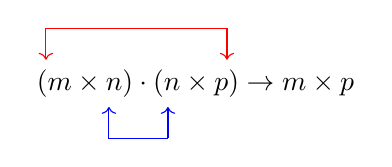
\begin{tikzpicture}
    % The matrix multiplication expression
    \node at (0,0) {\((m \times n) \cdot (n \times p) \rightarrow m \times p\)};
    
    % Red bidirectional U-shaped arrow on top
    \draw[red,<-] (-1.9,0.3) -- (-1.9,0.7) -- (0.4,0.7);
    \draw[red,->] (0.4,0.7) -- (0.4,0.3);
    
    % Blue bidirectional U-shaped arrow on the bottom
    \draw[blue,<-] (-1.1,-0.3) -- (-1.1,-0.7) -- (-0.35,-0.7);
    \draw[blue,->] (-0.35,-0.7) -- (-0.35,-0.3);
\end{tikzpicture}
\]

The diagram shows that the number of columns in the first matrix must equal the number of rows in the second matrix (the \textcolor{blue}{blue arrow}). The result is a new matrix with the number of rows from the first matrix and the number of columns from the second matrix (the \textcolor{red}{red arrow}).

\begin{example}
    For $A$ and $B$ below compute $AB$ and $BA$.

    \[
    A=\left[\begin{array}{lll}
    1 & 2 & -2 \\
    1 & 1 & -3
    \end{array}\right], \quad B=\left[\begin{array}{cccc}
    -4 & 2 & 4 & -4 \\
    -1 & -5 & -3 & 3 \\
    -4 & -4 & -3 & -1
    \end{array}\right]
    \]
    
\end{example}

\begin{solution}
    First $A B=\left[\begin{array}{llll}A \vect{b_1} & A \vect{b_2} & A \vect{b_3} & A \vect{b_4}\end{array}\right]$ :

\[
\begin{aligned}
& A B=\left[\begin{array}{lll}
1 & 2 & -2 \\
1 & 1 & -3
\end{array}\right]\left[\begin{array}{cccc}
-4 & 2 & 4 & -4 \\
-1 & -5 & -3 & 3 \\
-4 & -4 & -3 & -1
\end{array}\right] \\
& = \vcenter{\hbox{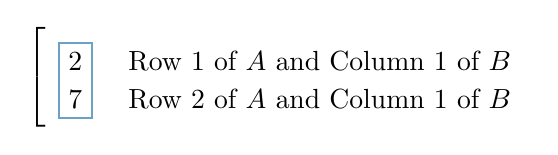
\begin{tikzpicture}
    \matrix (m1) [matrix of math nodes,left delimiter={[}] {
    2 & \quad \text{Row 1 of $A$ and Column 1 of $B$} \\
    7 & \quad \text{Row 2 of $A$ and Column 1 of $B$} \\
    };
    \draw[headercolor,thick] (m1-1-1.north west) rectangle (m1-2-1.south east);
\end{tikzpicture}}} \\
& = \vcenter{\hbox{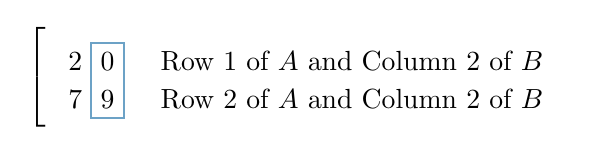
\begin{tikzpicture}
    \matrix (m2) [matrix of math nodes,left delimiter={[}] {
    2 & 0 & \quad \text{Row 1 of $A$ and Column 2 of $B$} \\
    7 & 9 & \quad \text{Row 2 of $A$ and Column 2 of $B$} \\
    };
    \draw[headercolor,thick] (m2-1-2.north west) rectangle (m2-2-2.south east);
\end{tikzpicture}}} \\
& = \vcenter{\hbox{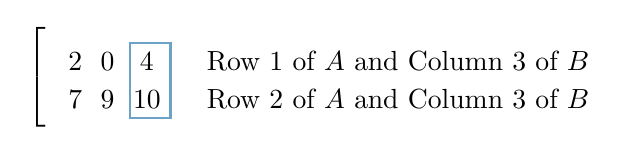
\begin{tikzpicture}
    \matrix (m3) [matrix of math nodes,left delimiter={[}] {
    2 & 0 & 4 & \quad \text{Row 1 of $A$ and Column 3 of $B$} \\
    7 & 9 & 10 & \quad \text{Row 2 of $A$ and Column 3 of $B$} \\
    };
    \draw[headercolor,thick] (m3-1-3.north west) rectangle (m3-2-3.south east);
\end{tikzpicture}}} \\
& = \vcenter{\hbox{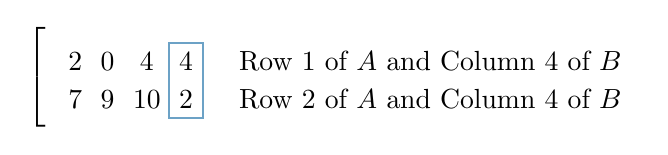
\begin{tikzpicture}
    \matrix (m4) [matrix of math nodes,left delimiter={[}] {
    2 & 0 & 4 & 4 & \quad \text{Row 1 of $A$ and Column 4 of $B$} \\
    7 & 9 & 10 & 2 & \quad \text{Row 2 of $A$ and Column 4 of $B$} \\
    };
    \draw[headercolor,thick] (m4-1-4.north west) rectangle (m4-2-4.south east);
\end{tikzpicture}}} \\
& = \vcenter{\hbox{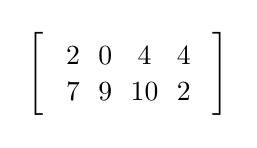
\begin{tikzpicture}
    \matrix (m4) [matrix of math nodes,left delimiter={[}, right delimiter={]}] {
    2 & 0 & 4 & 4 \\
    7 & 9 & 10 & 2 \\
    };
\end{tikzpicture}}}
\end{aligned}
\]

On the other hand, $B A$ is not defined! $B$ has 4 columns and $A$ has 2 rows. Thus, the number of columns in $B$ is not equal to the number of rows in $A$. \end{solution}

\begin{example}
    Example Compute the matrix $A B$, where

\[
A=\left[\begin{array}{ll}
1 & 2 \\
2 & 3 \\
3 & 4
\end{array}\right], \quad \text { and } B=\left[\begin{array}{cc}
2 & -1 \\
3 & 1
\end{array}\right]
\]

\end{example}

\begin{solution}
    By the definition of multiplication given above,

\[
\begin{aligned}
A B & =\left[A\left[\begin{array}{l}
2 \\
3
\end{array}\right] A\left[\begin{array}{c}
-1 \\
1
\end{array}\right]\right] \\
& \left.=\left[\begin{array}{ll}
1 & 2 \\
2 & 3 \\
3 & 4
\end{array}\right]\left[\begin{array}{l}
2 \\
3
\end{array}\right]\left[\begin{array}{ll}
1 & 2 \\
2 & 3 \\
3 & 4
\end{array}\right]\left[\begin{array}{c}
-1 \\
1
\end{array}\right]\right] \\
& =\left[\left[\begin{array}{l}
1 \cdot 2+2 \cdot 3 \\
2 \cdot 2+3 \cdot 3 \\
3 \cdot 2+4 \cdot 3
\end{array}\right]\left[\begin{array}{l}
1 \cdot(-1)+2 \cdot 1 \\
2 \cdot(-1)+3 \cdot 1 \\
3 \cdot(-1)+4 \cdot 1
\end{array}\right]\right] \\
& =\left[\begin{array}{cc}
8 & 1 \\
13 & 1 \\
18 & 1
\end{array}\right]
\end{aligned}
\]
\end{solution}

\begin{example} If $A$ is $3 \times 5$ and $B$ is $5 \times 2$, what are the sizes of $A B$ and $B A$ (assuming they are defined)?
\end{example}

\begin{solution}
    \begin{itemize}
        \item The product $A B$ is defined since the number of columns of $A$ matches the number of rows of $B$ (5). The resulting matrix $A B$ is a $3 \times 2$ matrix.
        \item The product $B A$ is not defined, since the number of columns of $B$ (2) does not match the number of rows of $A$ (3).
    \end{itemize}
\end{solution}

The next example illustrate that even if both $AB$ and $BA$ are defined, they are not necessarily equal.

\begin{example}
    For $A = \left[\begin{array}{rrr}
        -4 & 4 & 3 \\
        3 & -3 & -1 \\
        -2 & -1 & 1
        \end{array}\right] $ and $B = \left[\begin{array}{rrr}
            -1 & -1 & 0 \\
            -3 & 0 & -2 \\
            -2 & 1 & -2
            \end{array}\right]$ compute $AB$ and $BA$.

\end{example}

\begin{solution}
    First $AB$:

    \[
    \begin{aligned}
    A B &=\left[\begin{array}{rrr}
    -4 & 4 & 3 \\
    3 & -3 & -1 \\
    -2 & -1 & 1
    \end{array}\right]\left[\begin{array}{rrr}
    -1 & -1 & 0 \\
    -3 & 0 & -2 \\
    -2 & 1 & -2
    \end{array}\right] \\
    & =\left[\begin{array}{c}
    -14 \\
    8 \\
    3
    \end{array}\right. \\
    & =\left[\begin{array}{rr}
    -14 & 7 \\
    8 & -4 \\
    3 & 3
    \end{array}\right. \\
    & =\left[\begin{array}{rrr}
    -14 & 7 & -14 \\
    8 & -4 & 8 \\
    3 & 3 & 0
    \end{array}\right]
    \end{aligned}
    \]

    Next $BA$:
    \[
    \begin{aligned}
    B A & =\left[\begin{array}{rrr}
    -1 & -1 & 0 \\
    -3 & 0 & -2 \\
    -2 & 1 & -2
    \end{array}\right]\left[\begin{array}{rrr}
    -4 & 4 & 3 \\
    3 & -3 & -1 \\
    -2 & -1 & 1
    \end{array}\right] \\
    & =\left[\begin{array}{rrr}
    1 \\
    16 & \\
    15
    \end{array}\right. \\
    & =\left[\begin{array}{rrr}
    1 & -1 \\
    16 & -10 \\
    15 & -9
    \end{array}\right. \\
    & =\left[\begin{array}{rrr}
    1 & -1 & -2 \\
    16 & -10 & -11 \\
    15 & -9 & -9
    \end{array}\right]
    \end{aligned}
    \]

    We see that $AB \neq BA$. \end{solution}

    In regular arithmetic the multiplicative identity is 1. In matrix algebra, the multiplicative identity is the identity matrix, denoted by $I$. The identity matrix is a \textit{square} matrix with 1s on the diagonal and 0s elsewhere. The size of the identity matrix is determined by the context, and is usually clear from the context. For example, $I_2$ is a $2 \times 2$ identity matrix, and $I_3$ is a $3 \times 3$ identity matrix and in general $I_n \in \mathbb{R}^{n \times n}$ is an $n \times n$ identity matrix:

    $$
    I_n=\left[\begin{array}{ccccc}
    1 & 0 & 0 & \cdots & 0 \\
    0 & 1 & 0 & \cdots & 0 \\
    \vdots & \vdots & \vdots & \cdots & \vdots \\
    0 & 0 & 0 & \cdots & 1
    \end{array}\right]
    $$

    We can now state the following theorem.

    \begin{theorem}
        Let $A, B, C$ be matrices, of appropriate dimensions, and let $\alpha$ be a scalar. Then
\begin{enumerate}[(a)]
    \item $A(BC) = (AB)C$
    \item $A(B + C) = AB + AC$
    \item $(B + C)A = BA + CA$
    \item $\alpha(AB) = (\alpha A)B = A(\alpha B)$
    \item $I_n A = AI_n = A$
\end{enumerate}
\end{theorem}

We conclude this section by looking at the $k$th power of a matrix. \newpage

\begin{definition}
    Let $A$ be a square matrix, i.e. $ A \in \mathbb{R}^{n \times n}$. The $k$th power of $A$, denoted $A^k$, is defined as the product of $A$ with itself $k$ times. That is,

    $$
    A^k=\underbrace{ AAA \cdot \cdots A}_{k \text { times }}
    $$

    where $A$ appears $k$ times on the right-hand side.
\end{definition}

\begin{example}
    Compute $A^3$ if
    \[
    A=\left[\begin{array}{rr}
    -2 & 3 \\
    1 & 0
    \end{array}\right]
    \]
\end{example}

\begin{solution}

    Compute $A^2$ :

    \[
    A^2=\left[\begin{array}{rr}
    -2 & 3 \\
    1 & 0
    \end{array}\right]\left[\begin{array}{rr}
    -2 & 3 \\
    1 & 0
    \end{array}\right]=\left[\begin{array}{rr}
    7 & -6 \\
    -2 & 3
    \end{array}\right]
    \]

    And then $A^3$ :

    \[
    \begin{aligned}
    A^3=A^2 A & =\left[\begin{array}{rr}
    7 & -6 \\
    -2 & 3
    \end{array}\right]\left[\begin{array}{rr}
    -2 & 3 \\
    1 & 0
    \end{array}\right] \\
    & =\left[\begin{array}{rr}
    -20 & 21 \\
    7 & -6
    \end{array}\right]
    \end{aligned}
    \]

    We could also do:

    \[
    A^3=A A^2=\left[\begin{array}{rr}
    -2 & 3 \\
    1 & 0
    \end{array}\right]\left[\begin{array}{rr}
    7 & -6 \\
    -2 & 3
    \end{array}\right]=\left[\begin{array}{rr}
    -20 & 21 \\
    7 & -6
    \end{array}\right]
    \]

\end{solution}

\section{Matrix Transpose}
We begin with the definition of the transpose of a matrix.

\begin{definition}
    Given a matrix $A \in \mathbb{R}^{m \times n}$, the transpose of $A$ is the matrix $A^T$ whose $i$th column is the $i$th row of $A$.
\end{definition}

If $A$ is $m \times n$ then $A^T$ is $n \times m$. For example, if

\[
A=\left[\begin{array}{rrrrr}
0 & -1 & 8 & -7 & -4 \\
-4 & 6 & -10 & -9 & 6 \\
9 & 5 & -2 & -3 & 5 \\
-8 & 8 & 4 & 7 & 7
\end{array}\right]
\]

then

\[
A^T=\left[\begin{array}{rrrr}
0 & -4 & 9 & -8 \\
-1 & 6 & 5 & 8 \\
8 & -10 & -2 & 4 \\
-7 & -9 & -3 & 7 \\
-4 & 6 & 5 & 7
\end{array}\right]
\]

\begin{example} Compute $(AB)^T$ and $B^T A^T$ if

\[
A=\left[\begin{array}{rrr}
-2 & 1 & 0 \\
3 & -1 & -3
\end{array}\right], \quad B=\left[\begin{array}{rrr}
-2 & 1 & 2 \\
-1 & -2 & 0 \\
0 & 0 & -1
\end{array}\right].
\]
\end{example}

\begin{solution}
    First, compute $(AB)^T$:

    \[
    \begin{aligned}
    A B &=\left[\begin{array}{rrr}
    -2 & 1 & 0 \\
    3 & -1 & -3
    \end{array}\right]\left[\begin{array}{rrr}
    -2 & 1 & 2 \\
    -1 & -2 & 0 \\
    0 & 0 & -1
    \end{array}\right] \\
    &=\left[\begin{array}{rrr}
        3 & -4 & -4 \\
        -5 & 5 & 9
        \end{array}\right]
    \end{aligned}
    \]

    and then $(AB)^T$:

    \[
    \begin{aligned}
    (A B)^{T} &=\left[\begin{array}{rrr}
        3 & -4 & -4 \\
        -5 & 5 & 9
        \end{array}\right]^{T} \\
    &=\left[\begin{array}{rr}
        3 & -5 \\
        -4 & 5 \\
        -4 & 9
        \end{array}\right]
    \end{aligned}
    \]

    Next, compute $B^T A^T$:

    \[
    \begin{aligned}
    B^{T} A^{T} &=\left[\begin{array}{rrr}
        -2 & -1 & 0 \\
        1 & -2 & 0 \\
        2 & 0 & -1
        \end{array}\right]\left[\begin{array}{rr}
        -2 & 3 \\
        1 & -1 \\
        0 & -3
        \end{array}\right] \\
    &=\left[\begin{array}{rr}
    3 & -5 \\
    -4 & 5 \\
    -4 & 9
    \end{array}\right]
    \end{aligned}
    \]

    We see that $(AB)^T = B^T A^T$. \end{solution}

The following theorem summarises the properties of the transpose of a matrix.

\begin{theorem}
    Let $A$ and $B$ be matrices of appropriate dimensions and let $\alpha$ be a scalar. Then
    \begin{enumerate}[(a)]
        \item $(A^T)^T = A$
        \item $(A + B)^T = A^T + B^T$
        \item $(\alpha A)^T = \alpha A^T$
        \item $(AB)^T = B^T A^T$
    \end{enumerate}
\end{theorem}

A consequence of property (4) is that
\[
\left(A_1 A_2 \ldots A_k\right)^T=A_k^T A_{k-1}^T \cdots A_2^T A_1^T
\]

and as a special case

\[
\left(A^k\right)^T=\left(A^T\right)^k
\]

\section{Invertible Matrices}
The inverse of a square matrix \( A \in \mathbb{R}^{n \times n} \) extends the concept of the reciprocal for a nonzero real number \( a \in \mathbb{R} \). More precisely, the inverse of a non-zero number \( a \in \mathbb{R} \) is the unique number \( c \in \mathbb{R} \) such that \( a c = c a = 1 \). The inverse of \( a \neq 0 \), typically written as \( a^{-1} = \frac{1}{a} \), enables solving the equation \( a x = b \):

\[
a x = b \Rightarrow a^{-1} a x = a^{-1} b \Rightarrow x = a^{-1} b.
\]

This concept extends to square matrices, where the inverse of a matrix \( A \in \mathbb{R}^{n \times n} \) is a matrix \( C \in \mathbb{R}^{n \times n} \) such that \( A C = C A = I_n \), where \( I_n \) is the identity matrix of size \( n \times n \). The inverse of a matrix is denoted by \( A^{-1} \). We can now define the invertible matrix.

\begin{definition}
    A square matrix \( A \in \mathbb{R}^{n \times n} \) is invertible (or \textbf{nonsingular}) if there exists a matrix \( C \in \mathbb{R}^{n \times n} \) such that \( A C = C A = I_n \). The matrix \( C \) is called the inverse of \( A \) and is denoted by \( A^{-1} \). Thus, \( A^{-1} A = A A^{-1} = I_n \).
\end{definition}

\begin{example}
    Given $A$ and $C$ below, show that $C$ is the inverse of $A$.

    \[
    A=\left[\begin{array}{rrr}
    1 & -3 & 0 \\
    -1 & 2 & -2 \\
    -2 & 6 & 1
    \end{array}\right], \quad C=\left[\begin{array}{rrr}
    -14 & -3 & -6 \\
    -5 & -1 & -2 \\
    2 & 0 & 1
    \end{array}\right]
    \]
    \label{ex:inverse2}
\end{example}

\begin{solution}
    We need to show that $A C = C A = I_3$. First, compute $AC$:

    \[
    \begin{aligned}
    A C &=\left[\begin{array}{rrr}
    1 & -3 & 0 \\
    -1 & 2 & -2 \\
    -2 & 6 & 1
    \end{array}\right]\left[\begin{array}{rrr}
    -14 & -3 & -6 \\
    -5 & -1 & -2 \\
    2 & 0 & 1
    \end{array}\right] \\
    &=\left[\begin{array}{rrr}
    1 & 0 & 0 \\
    0 & 1 & 0 \\
    0 & 0 & 1
    \end{array}\right]=I_3
    \end{aligned}
    \]

    Next, compute $CA$:

    \[
    \begin{aligned}
    C A &=\left[\begin{array}{rrr}
    -14 & -3 & -6 \\
    -5 & -1 & -2 \\
    2 & 0 & 1
    \end{array}\right]\left[\begin{array}{rrr}
    1 & -3 & 0 \\
    -1 & 2 & -2 \\
    -2 & 6 & 1
    \end{array}\right] \\
    &=\left[\begin{array}{rrr}
    1 & 0 & 0 \\
    0 & 1 & 0 \\
    0 & 0 & 1
    \end{array}\right]=I_3
    \end{aligned}
    \]

    We see that $C=A^{-1}$ is the inverse of $A$. \end{solution}

The following theorem summarizes the relationship between the matrix inverse and matrix multiplication and matrix transpose.

\begin{theorem} Let $A$ and $B$ be invertible $n \times n$ matrices. Then:
\begin{enumerate}[(a)]
    \item $A^{-1}$ is invertible, with
    \[
    \left(A^{-1}\right)^{-1}=A
    \]
    \item The product $A B$ is invertible, with
    \[
    (A B)^{-1}=B^{-1} A^{-1}
    \]
    \item The transpose of $A$ is also invertible, i.e. $A^T$ is invertible, with
    \[
    \left(A^T\right)^{-1}=\left(A^{-1}\right)^T
    \]
\end{enumerate}

\end{theorem}

We will now consider how we can find the inverse of a matrix.

\subsection*{Finding the Determinant and Inverse of a $2 \times 2$ Matrix}

The inverse of a matrix is not always easy to find. However, for a $2 \times 2$ matrix, we can use a formula to find the inverse.

\begin{theorem}
    Let $A=\left[\begin{array}{ll}
    a & b \\
    c & d
    \end{array}\right]$. If $ad-bc \neq 0$, then the inverse of $A$ is given by

    \[
    A^{-1}=\frac{1}{ad-bc}\left[\begin{array}{cc}
    d & -b \\
    -c & a
    \end{array}\right]
    \]
\end{theorem}

\begin{remark}
    The quantity $ad - bc$ is called the determinant of $A$, and we write
    \[
    \text{det}(A) = |A| = ad - bc
    \]
\end{remark}

The determinant of a $2 \times 2$ matrix is a scalar quantity that provides information about the matrix. If the determinant is zero, then the matrix is not invertible. If the determinant is non-zero, then the matrix is invertible. These formulae are only valid $2 \times 2$ matrices.

\begin{example} We let

\[
A=\left[\begin{array}{ll}
1 & 2 \\
3 & 4
\end{array}\right]
\]

and compute $A^{-1}$. By the theorem, we have

\[
\begin{aligned}
A^{-1} & =\frac{1}{1 \cdot 4-2 \cdot 3}\left[\begin{array}{cc}
4 & -2 \\
-3 & 1
\end{array}\right] \\
& =-\frac{1}{2}\left[\begin{array}{cc}
4 & -2 \\
-3 & 1
\end{array}\right] \\
& =\left[\begin{array}{cc}
-2 & 1 \\
\frac{3}{2} & -\frac{1}{2}
\end{array}\right]
\end{aligned}
\]

Now we confirm that $A A^{-1}=I_2$ :

\[
\begin{aligned}
A A^{-1} & =\left[\begin{array}{ll}
1 & 2 \\
3 & 4
\end{array}\right]\left[\begin{array}{cc}
-2 & 1 \\
\frac{3}{2} & -\frac{1}{2}
\end{array}\right] \\
& =\left[\begin{array}{ll}
1(-2)+2\left(\frac{3}{2}\right) & 1(1)+2\left(-\frac{1}{2}\right) \\
3(-2)+4\left(\frac{3}{2}\right) & 3(1)+4\left(-\frac{1}{2}\right)
\end{array}\right] \\
& =\left[\begin{array}{ll}
-2+3 & 1-1 \\
-6+6 & 3-2
\end{array}\right] \\
& =\left[\begin{array}{ll}
1 & 0 \\
0 & 1
\end{array}\right]
\end{aligned}
\]
\label{ex:inverse}
\end{example}

\begin{example} Find the inverse of $A=\left[\begin{array}{cc}1 & 3 \\ -1 & -2\end{array}\right]$ if it exists.
    
\end{example}

\begin{solution}
    We first compute the determinant of $A$:

    \[
    \text{det}(A)=1(-2)-3(-1)=(-2)+3=1
    \]

    Since the determinant is non-zero, the inverse of $A$ exists. By the formula, we have

    \[
    \begin{aligned}
    A^{-1} & =\frac{1}{1}\left[\begin{array}{cc}-2 & -3 \\ 1 & 1\end{array}\right]
    \end{aligned}
    \]

    We can confirm that $A A^{-1}=I_2$:

    \[
        A A^{-1}=\left[\begin{array}{cc}
    1 & 3 \\
    -1 & -2
    \end{array}\right]\left[\begin{array}{cc}
    -2 & -3 \\
    1 & 1
    \end{array}\right]=\left[\begin{array}{ll}
    1 & 0 \\
    0 & 1
    \end{array}\right] =I_2
    \]

\end{solution}

For larger matrices, we need to use other methods to find the inverse.

\subsection*{Finding the Inverse of a $n \times n$ Matrix}
An \textbf{elementary matrix} is a matrix that is obtained by performing a single elementary row operation (replacement, swap, or scaling) on an identity matrix. For example, the matrix

\[
E_1=\left[\begin{array}{ccc}
1 & 0 & 0 \\
0 & 1 & 0 \\
-2 & 0 & 1
\end{array}\right]
\]

is an elementary matrix since it is obtained from $I_3$ via the single elementary row operation $r_3 \mapsto r_3-2 r_1$.

\begin{example}

Let $A$ be a general $3 \times 3$ matrix

\[
A=\left[\begin{array}{lll}
a & b & c \\
d & e & f \\
g & h & i
\end{array}\right]
\]

and we let $E_1, E_2$, and $E_3$ be the elementary matrices

\[
E_1=\left[\begin{array}{ccc}
1 & 0 & 0 \\
0 & 1 & 0 \\
-2 & 0 & 1
\end{array}\right], \quad E_2=\left[\begin{array}{lll}
1 & 0 & 0 \\
0 & 0 & 1 \\
0 & 1 & 0
\end{array}\right], \quad \text { and } \quad E_3=\left[\begin{array}{lll}
1 & 0 & 0 \\
0 & 3 & 0 \\
0 & 0 & 1
\end{array}\right]
\]
\end{example}

Notice, then, that $E_1$ corresponds to $r_3 \mapsto r_3-2 r_1, E_2$ corresponds to $r_2 \longleftrightarrow r_3$, and $E_3$ corresponds to $r_2 \mapsto 3 r_2$. We also have the following products:

\[
E_1 A=\left[\begin{array}{ccc}
a & b & c \\
d & e & f \\
g-2 a & h-2 b & i-2 c
\end{array}\right], \quad E_2 A=\left[\begin{array}{ccc}
a & b & c \\
g & h & i \\
d & e & f
\end{array}\right], \quad \text { and } \quad E_3 A=\left[\begin{array}{ccc}
a & b & c \\
3 d & 3 e & 3 f \\
g & h & i
\end{array}\right] .
\]


Notice that $E_1 A$ is the matrix obtained by performing the row operation $r_3 \mapsto r_3-2 r_1$ on $A$. In general, multiplying $A$ on the left by an elementary matrix is the same as performing the corresponding row operation on $A$. We can also represent a sequence of row operations by multiplication of several elementary matrices. For example,

\[
E_2 E_1 A=\left[\begin{array}{ccc}
a & b & c \\
g-2 a & h-2 b & i-2 c \\
d & e & f
\end{array}\right]
\]

corresponds to performing $r_3 \mapsto r_3-2 r_1$ followed by $r_2 \longleftrightarrow r_3$ on the matrix $A$.
As we have observed before, row operations are reversible. It follows that elementary matrices are also invertible. This leads to the following theorem.

\begin{theorem}
    An $n \times n$ matrix $A$ is invertible if and only if $A$ is row equivalent to $I_n$. In this case, any sequence of elementary row operations that reduces $A$ to $I_n$ also transforms $I_n$ into $A^{-1}$.
\end{theorem}

This theorem leads to a nice algorithm for finding the inverse of an $n \times n$ matrix, assuming such an inverse exists.

\begin{custombox}{Algorithm for Finding the Inverse of an $n \times n$ Matrix}
    Let $A$ be an $n \times n$ matrix. To find the inverse of $A$, follow these steps:
    \begin{enumerate}
        \item Form the augmented matrix $[A | I_n]$.
        \item Perform row operations on $[A | I_n]$ to reduce $A$ to $I_n$.
        \item The matrix on the right side of the augmented matrix is $A^{-1}$.
    \end{enumerate}

    If $A$ is not invertible, then the algorithm will not be able to reduce $A$ to $I_n$.
\end{custombox}

\begin{example} Find the inverse of $A=\left[\begin{array}{rrr}1 & 0 & 3 \\ 1 & 1 & 0 \\ -2 & 0 & -7\end{array}\right]$ if it exists.    
\end{example}

\begin{solution}
    Solution. Form the augmented matrix $\left[\begin{array}{ll}A & I_3\end{array}\right]$ and row reduce:
\[
\begin{alignedat}{3}
& \left[\begin{array}{cccccc}
1 & 0 & 3 & 1 & 0 & 0 \\
1 & 1 & 0 & 0 & 1 & 0 \\
-2 & 0 & -7 & 0 & 0 & 1
\end{array}\right]
& \quad & \begin{aligned}
    r_2 &\mapsto -r_1 + r_2 \\
    r_3 &\mapsto 2 r_1 + r_3
\end{aligned}
& \quad & \left[\begin{array}{cccccc}
1 & 0 & 3 & 1 & 0 & 0 \\
0 & 1 & -3 & -1 & 1 & 0 \\
0 & 0 & -1 & 2 & 0 & 1
\end{array}\right] \\[10pt]
& & \quad & r_3 \mapsto -r_3
& \quad & \left[\begin{array}{cccccc}
1 & 0 & 3 & 1 & 0 & 0 \\
0 & 1 & -3 & -1 & 1 & 0 \\
0 & 0 & 1 & -2 & 0 & -1
\end{array}\right] \\[10pt]
& & \quad & \begin{aligned}
    r_2 &\mapsto 3 r_3 + r_2 \\
    r_1 &\mapsto -3 r_3 + r_1
\end{aligned}
& \quad & \left[\begin{array}{cccccc}
1 & 0 & 0 & 7 & 0 & 3 \\
0 & 1 & 0 & -7 & 1 & -3 \\
0 & 0 & 1 & -2 & 0 & -1
\end{array}\right]
\end{alignedat}
\]

Therefore, \(\operatorname{rref}A = I_3\), confirming that \( A \) is invertible. The inverse is
\[
A^{-1} = \left[\begin{array}{ccc}
7 & 0 & 3 \\
-7 & 1 & -3 \\
-2 & 0 & -1
\end{array}\right]
\]
Verify:
\[
AA^{-1}=\left[\begin{array}{ccc}
1 & 0 & 3 \\
1 & 1 & 0 \\
-2 & 0 & -7
\end{array}\right]\left[\begin{array}{ccc}
7 & 0 & 3 \\
-7 & 1 & -3 \\
-2 & 0 & -1
\end{array}\right]=\left[\begin{array}{lll}
1 & 0 & 0 \\
0 & 1 & 0 \\
0 & 0 & 1
\end{array}\right]
\]

\end{solution}

\begin{example}
    Find the inverse of $A=\left[\begin{array}{rrr}1 & 0 & 1 \\ 1 & 1 & -2 \\ -2 & 0 & -2\end{array}\right]$ if it exists.
\end{example}

\begin{solution}
    Form the augmented matrix $\left[\begin{array}{ll}A & I_3\end{array}\right]$ and row reduce:
\[
\begin{alignedat}{3}
& \left[\begin{array}{cccccc}
1 & 0 & 1 & 1 & 0 & 0 \\
1 & 1 & -2 & 0 & 1 & 0 \\
-2 & 0 & -2 & 0 & 0 & 1
\end{array}\right]
& \quad & \begin{aligned}
    r_2 &\mapsto -r_1 + r_2 \\
    r_3 &\mapsto 2 r_1 + r_3
\end{aligned}
& \quad & \left[\begin{array}{cccccc}
1 & 0 & 1 & 1 & 0 & 0 \\
0 & 1 & -3 & -1 & 1 & 0 \\
0 & 0 & 0 & 2 & 0 & 1
\end{array}\right]
\end{alignedat}
\]

We need not go further since the rref($A$) is not $I_3$. Therefore, A is not invertible.
\end{solution}

\begin{example}
    Find the inverse of the matrix

    \[
    A=\left[\begin{array}{lll}
        1 & 2 & 1 \\
        4 & 5 & 3 \\
        0 & 0 & 2
        \end{array}\right]
    \]
if it exists.
\end{example}

\begin{solution} (We ommit the row reduction steps for brevity.)
\[
\begin{aligned}
{\left[\begin{array}{llllll}
1 & 2 & 1 & 1 & 0 & 0 \\
4 & 5 & 3 & 0 & 1 & 0 \\
0 & 0 & 2 & 0 & 0 & 1
\end{array}\right] } & \sim\left[\begin{array}{cccccc}
1 & 2 & 1 & 1 & 0 & 0 \\
0 & -3 & -1 & -4 & 1 & 0 \\
0 & 0 & 2 & 0 & 0 & 1
\end{array}\right] \\
& \sim\left[\begin{array}{cccccc}
1 & 2 & 1 & 1 & 0 & 0 \\
0 & -3 & -1 & -4 & 1 & 0 \\
0 & 0 & 1 & 0 & 0 & \frac{1}{2}
\end{array}\right] \\
& \sim\left[\begin{array}{cccccc}
1 & 2 & 0 & 1 & 0 & -\frac{1}{2} \\
0 & -3 & 0 & -4 & 1 & \frac{1}{2} \\
0 & 0 & 1 & 0 & 0 & \frac{1}{2}
\end{array}\right] \\
& \sim\left[\begin{array}{cccccc}
1 & 2 & 0 & 1 & 0 & -\frac{1}{2} \\
0 & 1 & 0 & \frac{4}{3} & -\frac{1}{3} & -\frac{1}{6} \\
0 & 0 & 1 & 0 & 0 & \frac{1}{2}
\end{array}\right] \\
& \sim\left[\begin{array}{cccccc}
1 & 0 & 0 & -\frac{5}{3} & \frac{2}{3} & -\frac{1}{6} \\
0 & 1 & 0 & \frac{4}{3} & -\frac{1}{3} & -\frac{1}{6} \\
0 & 0 & 1 & 0 & 0 & \frac{1}{2}
\end{array}\right] .
\end{aligned}
\]

Hence

\[
A^{-1}=\left[\begin{array}{ccc}
-\frac{5}{3} & \frac{2}{3} & -\frac{1}{6} \\
\frac{4}{3} & -\frac{1}{3} & -\frac{1}{6} \\
0 & 0 & \frac{1}{2}
\end{array}\right] .
\]

\end{solution}

With the method for finding matrix inverses established, we now have a powerful tool for approaching linear systems. We will see how matrix inverses can be used to solve systems of equations efficiently, offering a straightforward way to find solutions when a matrix is invertible.

\subsection*{Solving Matrix Equations with Inverses}
Just like we can solve an equation by using the reciprocal of a non-zero number as we saw previously, we can do something similar with matrices. When a matrix \( A \) is invertible, we can use its inverse to solve matrix equations involving \( A \). This brings us to the theorem below, which shows how we can find solutions for equations like \( A \vect{x} = \vect{b} \) when \( A \) has an inverse.

\begin{theorem}
    Let \( A \) be an invertible matrix. Then the equation \( A \vect{x} = \vect{b} \) has a unique solution given by \( \vect{x} = A^{-1} \vect{b} \).
\end{theorem}

\begin{example}
We can use the inverse from example \ref{ex:inverse} to solve the linear system

\[
\begin{aligned}
x_1+2 x_2 & =5 \\
3 x_1+4 x_2 & =6 .
\end{aligned}
\]

We think of this in matrix terms as \(A \vect{x}=\vect{b}\), where

\[
A=\left[\begin{array}{ll}
1 & 2 \\
3 & 4
\end{array}\right], \quad \vect{x}=\left[\begin{array}{l}
x_1 \\
x_2
\end{array}\right], \quad \text { and } \quad \vect{b}=\left[\begin{array}{l}
5 \\
6
\end{array}\right]
\]

The theorem tells us that \(\vect{x}=A^{-1} \vect{b}\) is a solution, i.e. that

\[
\begin{aligned}
{\left[\begin{array}{l}
x_1 \\
x_2
\end{array}\right] } & =\left[\begin{array}{cc}
-2 & 1 \\
\frac{3}{2} & -\frac{1}{2}
\end{array}\right]\left[\begin{array}{l}
5 \\
6
\end{array}\right] \\
& =\left[\begin{array}{c}
-2(5)+1(6) \\
\frac{3}{2}(5)-\frac{1}{2}(6)
\end{array}\right] \\
& =\left[\begin{array}{c}
-4 \\
\frac{9}{2}
\end{array}\right]
\end{aligned}
\]
\end{example}

\begin{example} Use the result from example \ref{ex:inverse2} to solve the linear system $A \vect{x} = \vect{b}$ where

    \[A=\left[\begin{array}{rrr}1 & -3 & 0 \\ -1 & 2 & -2 \\ -2 & 6 & 1\end{array}\right], \quad \vect{b}=\left[\begin{array}{c}1 \\ -3 \\ -1\end{array}\right]\]

\end{example}

\begin{solution} We showed in example \ref{ex:inverse2} that

    \[
    A^{-1}=\left[\begin{array}{rrr}
    -14 & -3 & -6 \\
    -5 & -1 & -2 \\
    2 & 0 & 1
    \end{array}\right]
    \]

Therefore, the unique solution to the linear system $A \vect{x} = \vect{b}$ is

    \[
    A^{-1} \vect{b}=\left[\begin{array}{rrr}
    -14 & -3 & -6 \\
    -5 & -1 & -2 \\
    2 & 0 & 1
    \end{array}\right]\left[\begin{array}{c}
    1 \\
    -3 \\
    -1
    \end{array}\right]=\left[\begin{array}{l}
    1 \\
    0 \\
    1
    \end{array}\right]
    \]

Verify:

    \[
    \left[\begin{array}{rrr}
    1 & -3 & 0 \\
    -1 & 2 & -2 \\
    -2 & 6 & 1
    \end{array}\right]\left[\begin{array}{l}
    1 \\
    0 \\
    1
    \end{array}\right]=\left[\begin{array}{c}
    1 \\
    -3 \\
    -1
    \end{array}\right]
    \]
\end{solution}

We conclude this chapter with one of the most important theorems in linear algebra, The Invertible Matrix Theorem.

\section{The Invertible Matrix Theorem}

The Invertible Matrix Theorem provides a comprehensive list of equivalent statements for a square matrix to be invertible and it enables us to determine the truth value of one statement by checking the truth value of another.

\newpage

\begin{theorem}
    Let \( A \) be an \( n \times n \) matrix. The following statements are equivalent:
    \begin{enumerate}[(a)]
        \item $A$ is invertible.
        \item $A$ is row equivalent to $I_n$.
        \item $A$ has $n$ pivot positions (i.e. one for each row and column).
        \item The equation $A \vect{x}=\overline{0}$ has only the trivial solution.
        \item The columns of $A$ are linearly independent.
        \item The equation \( A \vect{x} = \vect{b} \) has a unique solution for each \( \vect{b} \in \mathbb{R}^n \).
        \item The columns of $A \operatorname{span} \mathbb{R}^n$.
        \item \( \text{det}(A) \neq 0 \).
        \item There is an $n \times n$ matrix $C$ such that $C A=I$.
        \item There is an $n \times n$ matrix $D$ such that $A D=I$.
        \item $A^T$ is invertible.
    \end{enumerate}
\end{theorem}

Note how the theorem connects the properties of a matrix to its invertibility, thus summarising the main elements of our discussion on linear systems, independence, vectors, and matrices.

\begin{example} Decide if the following matrix is invertible:

\[
A=\left[\begin{array}{lll}
2 & 2 & 2 \\
1 & 3 & 1 \\
4 & 4 & 6
\end{array}\right]
\]

\end{example}

\begin{solution}
Performing row operations, we see

\[
\begin{aligned}
A & \sim\left[\begin{array}{lll}
1 & 3 & 1 \\
2 & 2 & 2 \\
4 & 4 & 6
\end{array}\right] \\
& \sim\left[\begin{array}{ccc}
1 & 3 & 1 \\
0 & -4 & 0 \\
0 & -8 & 2
\end{array}\right] \\
& \sim\left[\begin{array}{ccc}
1 & 3 & 1 \\
0 & -4 & 0 \\
0 & 0 & 2
\end{array}\right]
\end{aligned}
\]
which has 3 pivots, so by (c) we have that $A$ is invertible.
\end{solution}

This concludes our discussion on matrices.
% \chapter{Time Complexity}\label{chap:ch10}

When discussing the efficiency of an algorithm, we aim to understand how it scales with input size, abstracting away details of specific hardware or programming environments. \textit{Theoretical} time complexity, commonly represented by Big-$\mathcal{O}$ notation (with a capital $\mathcal{O}$, not a zero), enables this abstraction by focusing on the dominant terms of an algorithm's behaviour as inputs grow large. This notation, also known as Landau's symbol, was introduced by the German number theorist Edmund Landau, with $\mathcal{O}$, standing for "order," capturing the growth rate of a function.

This chapter will introduce the tools needed to analyse algorithmic efficiency using Big-$\mathcal{O}$, Omega ($\Omega$), and Theta ($\Theta$) notation.\footnote{In practice, Big-$\mathcal{O}$ is often used informally as an umbrella term when discussing asymptotic analysis in a general sense, but it does not technically include $\Theta$ or $\Omega$. Each notation has its own specific use case in bounding the function's growth rate from different perspectives (upper, lower, and tight bounds), as we will see shortly.}

\section{Introduction to Complexity Analysis}\label{sec:ch10sec1}

For instance, analysing an algorithm might reveal that the time it takes to complete a problem of size $n$ is given by $T(n)=4 n^2-2 n+2$. By ignoring constants — since these vary with hardware and slower-growing terms - we simplify this to $T(n)=O\left(n^2\right)$, emphasizing the dominant term. This abstraction helps us understand complexity on large inputs, regardless of specific environments, making Big-$\mathcal{O}$ a powerful tool for comparing algorithms.

The two key components of this theoretical abstraction are:

\begin{enumerate}
    \item \textbf{Ignoring multiplicative constants:} Constants often depend on factors like processor speed or compiler optimisations, making them impractical for broad analysis.
    \item \textbf{Focusing on asymptotic behaviour:} We concentrate on the algorithm's behaviour with large inputs, as small cases typically run fast on any modern machine.
\end{enumerate}

However, in \textit{practical} time complexity, every term — including constants — plays a role. When running code on specific hardware with a known environment, those "negligible" constants in Big-$\mathcal{O}$ can become significant, especially for algorithms applied to small- and medium-sized data sets. So, while Big-$\mathcal{O}$ is crucial for high-level analysis and comparing algorithms, real-world complexity often requires looking at every term in the complexity expression. The following example illustrates this concept.

\begin{lstlisting}[style=pythonStyle, caption={Linear Search in Python}, label={lst:python_linear_search}]
    def linear_search(arr, target):
        for i in range(len(arr)):
            if arr[i] == target:
                return i
        return -1
\end{lstlisting} \newpage
    
% Use Java style for a Java code listing
\begin{lstlisting}[style=javaStyle, caption={Linear Search in Java}, label={lst:java_linear_search}]
    public static int linearSearch(int[] arr, int target) {
        for (int i = 0; i < arr.length; i++) {
            if (arr[i] == target) {
                return i;
            }
        }
        return -1;
    }
\end{lstlisting}

This code performs a linear search through a list, checking each element until it finds the target or reaches the end of the list. Here, the time complexity is $\mathcal{O}(n)$ in the worst case, as every element must be checked. For small lists, the difference may be negligible, but as the input size grows, the linear relationship between input size and runtime becomes evident.

When we ask "How efficient is an algorithm or piece of code?", we note that efficiency encompasses various resources, including:
\begin{itemize}
    \item CPU (time) usage
    \item Memory usage
    \item Disk usage
    \item Network usage
\end{itemize}

While all these resources are important, this chapter will primarily focus on time complexity, which concerns CPU usage.

\begin{enumerate}
    \item \textbf{Performance:} This refers to how much time, memory, disk space, or other resources are actually used when a program is run. Performance is influenced by factors such as the machine, compiler, runtime environment, and other implementation details in addition to the code itself.
    \item \textbf{Complexity:} Complexity, on the other hand, describes how the resource requirements of a program or algorithm scale with the size of the problem being solved. Complexity analysis focuses on the theoretical aspects of algorithm performance, characterizing how resource usage grows as input size increases.
\end{enumerate}

Complexity impacts performance, but performance alone does not provide a complete picture of an algorithm's efficiency in terms of scalability. Understanding both is crucial to evaluating how well an algorithm will perform in diverse realworld scenarios, especially as input sizes grow significantly.

\section{Growth of Functions}
In Section \ref{sec:ch10sec1}the introduction to this chapter we noted that Big-$\mathcal{O}$ notation focuses on the dominant term of an algorithm's time complexity, abstracting away constants and smaller terms. This simplification is based on the idea that, as input sizes grow large, the dominant term will dictate the algorithm's complexity. Consider the following Java code snippet:

\newpage

\begin{lstlisting}[style=javaStyle, caption={Java SumCalculator}, label={lst:java_f_function}]
    public static int f(int n) {
        int sum = 0;
        for (int i = 0; i < n; i++) {
            for (int j = 0; j < n; j++) {
                sum += (i + j) / 6;
            }
        }
        return sum;
    }
\end{lstlisting}

The code above is an implementation of the following expression:

\[
\operatorname{sum}=\sum_{i=0}^{n-1} \sum_{j=0}^{n-1} \frac{i+j}{6}
\]

Assuming $n$ is a non-negative integer, let $T(n)$ represent the CPU time taken by a typical laptop to execute the function\footnote{In Java, it's technically a method, not a function. In Java terminology, a function that belongs to a class (the function would probably belong to a class such as \inlinecode{public class SumCalculator}) is called a method. A function generally refers to a standalone block of code that can be invoked independently, which is typical in languages like C or Python.}  $f(n)$, with input $n$. Naturally, $T(n)$ can vary due to factors that we may not fully control, such as the specific Java compiler, the hardware specifications of the laptop, the operating system, and other applications running simultaneously. However, we can be certain of the structure of the loops: the outer loop runs $n$ times, and for each outer iteration, the inner loop also runs $n$ times, resulting in a total of $n^2$ iterations. 

Each iteration requires an approximate constant number of clock cycles, denoted \( c \), which can differ depending on the system. Instead of stating that "$T(n)$ is approximately \( cn^2 \) nanoseconds, for some constant \( c \) that varies across systems," we use Big-$\mathcal{O}$ notation to write \( T(n) = \mathcal{O}(n^2) \). This notation captures the idea that the CPU time grows at most quadratically with \( n \). To visualize this, consider a graph of \( T(n) \), which would generally appear parabolic with an approximate form of \( cn^2 \), where \( c > 0 \) is constant.

\begin{figure}[htbp]
    \centering
    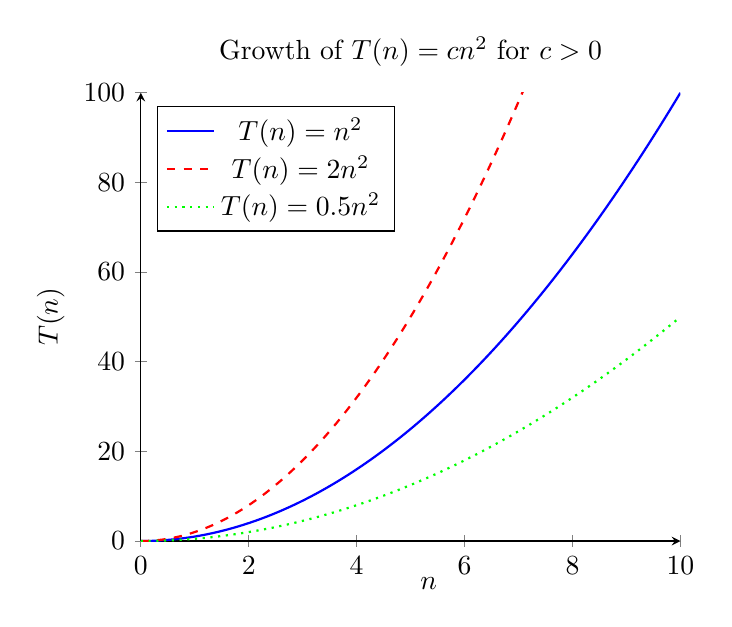
\begin{tikzpicture}
        \begin{axis}[
            domain=0:10,
            samples=100,
            axis lines=left,
            xlabel={$n$},
            ylabel={$T(n)$},
            ymin=0, ymax=100,
            xmin=0, xmax=10,
            xtick={0,2,4,6,8,10},
            ytick={0,20,40,60,80,100},
            xlabel style={right},
            ylabel style={above},
            legend pos=north west,
            title={Growth of $T(n) = cn^2$ for $c > 0$}
        ]
            \addplot[blue, thick] {x^2};
            \addlegendentry{$T(n) = n^2$}

            \addplot[red, thick, dashed] {2*x^2};
            \addlegendentry{$T(n) = 2n^2$}

            \addplot[green, thick, dotted] {0.5*x^2};
            \addlegendentry{$T(n) = 0.5n^2$}
        \end{axis}
    \end{tikzpicture}
    \caption{Graph of $T(n) = cn^2$ illustrating quadratic growth for different values of $c$}
    \label{fig:quadratic_growth}
\end{figure}

Big-$\mathcal{O}$ notation enables us to disregard constants, which often vary and lie beyond our control, yet do not affect the "family" or general growth rate classification of the function. For example, any potential $T(n)$ function in this case falls into the family of quadratic functions as illustrated in Figure \ref{fig:quadratic_growth}. Additionally, lower-order terms become insignificant for large $n$ as they can be bounded by a constant multiple of the dominant term. 

For instance, if $f(n) = 3.5n^2 + 4n + 36$, we observe that $f(n) \geq 3.5n^2$. Simultaneously,

\[
f(n) = 3.5n^2 + 4n + 36 \leq 3.5n^2 + 4n^2 + 36n^2 = 43.5n^2,
\]

which effectively "sandwiches" $f(n)$ between two quadratic functions, confirming that its growth is essentially quadratic.

\subsection*{Primitive Functions}
To understand how functions grow, let’s arrange some fundamental functions by their growth rates. We are looking for relationships of the form \( f(n) \leq g(n) \), but since we only care about behaviour with large inputs, these relationships hold only beyond some lower bound \( k \) for \( n \).

Starting with the basics, any constant function grows more slowly than a linear function, simply because a constant does not grow at all. For large enough values, a linear function grows slower than a quadratic, while a cubic function grows faster than a quadratic.

Exponentials are well known for their rapid growth. Consider the tale of a company that decided to reward an employee by doubling their bonus each day for a month. Although it started with a modest amount, the exponential increase quickly escalated, and by the end of the month, the bonus would have been astronomical. Realizing the unsustainable cost, the company swiftly revised the agreement to a fixed rate instead. Mathematically, this effect is clear: \( n^2 < 2^n \) for any integer \( n \geq 4 \). More generally, for any exponent \( k \), \( n^k < 2^n \) for sufficiently large \( n \).

Even more dramatically, factorial growth, represented by \( n! \), outpaces exponential growth for large \( n \). The reasoning is that \( 2^n \) consists of \( n \) factors of 2, while \( n! \) includes the first \( n \) integers as factors, most of which are larger than 2. Thus, \( n! \) eventually grows faster than \( 2^n \). 

To summarize, exponential growth is faster than any polynomial growth, and factorial growth surpasses both. Using \(1\) as our constant function, we can express these relationships as:

\[
1 \prec n \prec n^2 \prec n^3 \ldots \prec 2^n \prec n!
\]

The symbol \( \prec \) is used here because this ordering is not a standard algebraic inequality and only applies when \( n \) is sufficiently large.

For designing computer programs, only the first few of these growth rates are practical. Third-order polynomials can already grow too quickly for larger inputs, and exponential-time algorithms are only feasible for very small cases. Often, exponential algorithms are replaced by faster, approximate methods such as statistical sampling.

Now, let's consider functions with slower growth — these are the types of functions we aim for in efficient algorithms. Algorithms for searching in large datasets often have running times proportional to \( \log n \). If we plot \( \log n \) for values greater than 1, it shows slow but consistent growth, much slower than \( n \) itself.

\begin{figure}[htbp]
    \centering
    \begin{tikzpicture}
        \begin{axis}[
            domain=1:10,
            samples=100,
            axis lines=left,
            xlabel={$n$},
            ylabel={$T(n)$},
            ymin=0, ymax=12,
            xmin=1, xmax=10,
            xtick={1,2,4,6,8,10},
            ytick={0,2,4,6,8,10,12},
            xlabel style={right},
            ylabel style={above},
            legend pos=north west,
            title={Growth of $\log n$ vs. $n$}
        ]
            % Plot for log(n)
            \addplot[blue, thick] {ln(x)};
            \addlegendentry{$\log n$}

            % Plot for n
            \addplot[red, thick, dashed] {x};
            \addlegendentry{$n$}
        \end{axis}
    \end{tikzpicture}
    \caption{Graph comparing the growth rates of $\log n$ and $n$}
\end{figure}

Sorting algorithms, on the other hand, often have running times proportional to \( n \log n \). For large \( n \), we observe that \( 1 < \log n < n \), leading to \( n < n \log n < n^2 \). This order can be summarized as:

\[
1 \prec \log n \prec n \prec n \log n \prec n^2
\]

\begin{remark}
    When discussing $\log n$, we typically refer to the base-2 logarithm, as it is the most common in computer science and software engineering. However, the base of the logarithm does not affect the growth rate, as it only introduces a constant factor. For example, $\log_2 n$ and $\log_{10} n$ grow at the same rate, differing only by a constant multiple.
\end{remark}

\begin{table}[htbp]
    \centering
    \renewcommand{\arraystretch}{1.4}
    \begin{tabular}{|c|l|l|}
        \hline
        \textbf{Complexity} & \textbf{Growth Rate} & \textbf{Example Algorithms} \\
        \hline
        \( \mathcal{O}(1) \) & Constant & Accessing an array element \\
        \hline
        \( \mathcal{O}(\log n) \) & Logarithmic & Binary search \\
        \hline
        \( \mathcal{O}(n) \) & Linear & Linear search \\
        \hline
        \( \mathcal{O}(n \log n) \) & Linearithmic (or Log-Linear) & MergeSort, QuickSort, HeapSort \\
        \hline
        \( \mathcal{O}(n^2) \) & Quadratic & Bubble Sort, Selection Sort \\
        \hline
        \( \mathcal{O}(n^3) \) & Cubic & Matrix multiplication \\
        \hline
        \( \mathcal{O}(n^k) \) & Polynomial & Polynomial-time approximation algorithms \\
        \hline
        \( \mathcal{O}(c^n) \) & Exponential & Subset sum, brute force for combinatorial problems \\
        \hline
        \( \mathcal{O}(n!) \) & Factorial & Brute force for travelling salesperson \\
        \hline
        \( \mathcal{O}(n^n) \) & Super-exponential & Recursive algorithms with high branching factor \\
        \hline
    \end{tabular}
    \caption{Growth rates of common functions and example algorithms}
    \label{tab:growth_rates}
\end{table}


Table \ref{tab:growth_rates} summarizes the growth rates of common functions and supply some examples of algorithms that exhibit these growth rates and Figure \ref{fig:time_complexities} provides a visual representation of these growth rates. Memorizing the relative order of these common functions is valuable, as they will reappear frequently in this and other software engineering contexts.

\begin{figure}[htbp]
    \centering
    \begin{tikzpicture}
        % Draw axes
        \draw[->] (0,0) -- (0,5) node[midway, rotate = 90, anchor = south] {Time Complexity};
        \draw[->] (0,0) -- (6,0) node[below, midway] {Input Size};

        % Draw conceptual growth curves
        \draw[thick, green!70!black] plot [domain=0:6] (\x, {0.5}) node[right] {$\mathcal{O}(1)$};
        \draw[thick, green] plot [domain=0:6] (\x, {0.5*ln(\x+1)}) node[right] {$\mathcal{O}(\log n)$};
        \draw[thick, lime!80!black] plot [domain=0:6] (\x, {0.5*\x}) node[right] {$\mathcal{O}(n)$};
        \draw[thick, yellow!70!orange] plot [domain=0:6] (\x, {0.35*\x*ln(\x+1)}) node[right] {$\mathcal{O}(n \log n)$};
        \draw[thick, orange] plot [domain=0:5] (\x, {0.2*\x^2}) node[right] {$\mathcal{O}(n^2)$};
        \draw[thick, red!60!orange] plot [domain=0:4] (\x, {0.08*\x^3}) node[above right] {$\mathcal{O}(n^3)$};
        
        % Make O(2^n) and O(n!) much steeper
        \draw[thick, red!80!black] plot [domain=0:2.7] (\x, {0.2*exp(\x*1.2)}) node[above right] {$\mathcal{O}(c^n)$};
        \draw[thick, red!40!black] plot [domain=0:1.45] (\x, {0.28*exp(\x*2)}) node[above right] {$\mathcal{O}(n!)$};
        \draw[thick, black] plot [domain=0:0.83] (\x, {0.08*exp(\x*5)}) node[above] {$\mathcal{O}(n^n)$};

    \end{tikzpicture}
    \caption{Conceptual illustration of time complexities}
    \label{fig:time_complexities}
\end{figure}

In the next section, we introduce the framework for analysing algorithms using Big-$\mathcal{O}$, Omega ($\Omega$), and Theta ($\Theta$) notation, which allows us to describe the growth behaviour of functions more precisely. These notations correspond to the worst-case, best-case, and tight bounds of an algorithm's time complexity, respectively. Note that Theta ($\Theta$) notation is used when the upper and lower bounds of an algorithm's runtime are asymptotically the same, providing a precise description of the algorithm's complexity across different input sizes.


\section{Asymptotic Analysis}
In the analysis of algorithms, Big-$\mathcal{O}$, Omega ($\Omega$), and Theta ($\Theta$) notation each offer a unique perspective on an algorithm's efficiency, helping us understand how it will perform under different conditions. Whether we aim to determine the upper bound (worst-case scenario), lower bound (best-case scenario), or a tight bound, we can generally follow a systematic approach as follows:

\begin{enumerate}
    \item \textbf{Identify the Dominant Operations:} Focus on the operations that contribute most significantly to the running time, particularly those that grow the fastest as the input size increases.
    
    \item \textbf{Discard Constants and Lower-Order Terms:} For Big-$\mathcal{O}$ and $\Theta$ notation, ignore constant factors and lower-order terms to concentrate on the term that dictates the overall growth rate. For $\Omega$, ensure that you establish a lower bound that is still representative of the growth rate.
    
    \item \textbf{Express Complexity in Terms of the Input Size:} Write the complexity using $n$, the input size. If the runtime is proportional to the square of the input size, express it as $\mathcal{O}(n^2)$ if analysing an upper bound, $\Omega(n^2)$ if analysing a lower bound, or $\Theta(n^2)$ if establishing a tight bound.
\end{enumerate}


\begin{example}

Consider the function, $f(n)=4 n^3+3 n^2+2 n+10$. Let us determine the worst-case scenario, Big-$\mathcal{O}$, using the systematic approach outlined.
    \begin{enumerate}
        \item \textbf{Identify the Dominant Operations:}
        \begin{itemize}
            \item Look at each term in $f(n)=4 n^3+3 n^2+2 n+10$.
            The terms $4 n^3, 3 n^2, 2 n$, and 10 contribute differently to the running time.
            As $n$ grows, the $4 n^3$ term will dominate the growth of the function because $n^3$ grows faster than $n^2, n$, and constant terms. Therefore, we focus on $4 n^3$.
        \end{itemize}
        \item \textbf{Discard Constants:}
        \begin{itemize}
            \item Ignore the constant coefficient 4 in $4 n^3$, as Big-$\mathcal{O}$ notation only considers the asymptotic growth rate.
            We can disregard the lower-order terms $3 n^2, 2 n$, and 10 since they do not impact the asymptotic behaviour as $n$ becomes very large.
        \end{itemize}
        \item \textbf{Express Complexity in Terms of the Input Size $n$:}
        \begin{itemize}
            \item With the constants and lower-order terms removed, we are left with $n^3$.
            Since $4 n^3$ dominates the growth, we describe the complexity in terms of $n^3$ for all three notations

            \[
                f(n)=\mathcal{O}\left(n^3\right)
            \]
        \end{itemize}
    \end{enumerate}
\end{example}

Similar considerations apply to the best-case scenario, Omega ($\Omega$), and the tight bound, Theta ($\Theta$). We now introduce the three notations more in depth, starting with the tight bound notation, Theta ($\Theta$).

\subsection*{Theta (\texorpdfstring{$\Theta$}{Theta}) Notation}

Theta notation provides a \textit{tight bound}, indicating that the growth rate of a function is bounded both above and below by the same asymptotic expression. In other words, $\Theta$ notation is used when the upper and lower bounds of an algorithm’s runtime are the same, describing the algorithm’s complexity consistently across different input sizes.

Mathematically, $T(n) = \Theta(f(n))$ if there exist constants $c_1, c_2 > 0$ and $k \geq 0$ such that $c_1 \cdot f(n) \leq T(n) \leq c_2 \cdot f(n)$ for all $n \geq k$.

We can summarize this in the following definition:

\begin{definition}{Theta(\(\Theta\))}
    $f(n)$ is $\Theta(g(n))$ if there exist positive constants $c_1, c_2$, and $k$ such that for all $n \geq k$,
    \medskip
    \[
    c_1 \cdot g(n) \leq f(n) \leq c_2 \cdot g(n)
    \]
    \medskip
This means that $f(n)$ is asymptotically bounded both above and below by $g(n)$, meaning that $f(n)$ grows at the same rate as $g(n)$ as $n$ becomes sufficiently large.
\label{def:theta_notation}
\end{definition}

Note that by writing "$n$ becomes sufficiently large" we mean that the above inequalities do not have to hold for all $n \geq 0$, but rather for all $n \geq k$, for some constant $k \geq 0$. Sometimes we provide an exact value for $k$, and other times use the "sufficiently large" phrase when the value of $k$ is not important.

\begin{figure}[htbp]
    \centering
    \begin{tikzpicture}
        % Axes
        \draw[->] (0,0) -- (5,0) node[right] {$n$};
        \draw[->] (0,0) -- (0,4.5) node[above] {};
        
        % Dashed line for n0
        \draw[dashed] (0.7,0) -- (0.7,2.5) node[below,yshift=-70pt] {$k$};

        % Plot for c1 * g(n) (lower bound) - Increase squiggles by lowering tension
        \draw[thick] plot[smooth, tension=0.6] coordinates {(0,0) (1,1) (2,0.7) (3, 1.3) (3.4, 2) (4,2.2)};
        \node at (4.65,2.2) {$c_1 g(n)$};

        % Plot for c2 * g(n) (upper bound) - Reduce squiggles by raising tension
        \draw[thick] plot[smooth, tension=1.0] coordinates {(0,0) (1,3) (2,3) (4,4)};
        \node at (4.65,4) {$c_2 g(n)$};

        % Plot for f(n) in between c1 g(n) and c2 g(n) - Fine-tuned squiggles by adjusting control points
        \draw[thick] plot[smooth, tension=0.8] coordinates {(0,0.7) (0.5,0.4) (1,1.3) (2.5,2.5) (3.5,3) (4,3.2)};
        \node at (4.5,3.2) {$f(n)$};
        
        % Label for Theta notation
        \node at (2.5,-0.5) {$f(n) = \Theta(g(n))$};
    \end{tikzpicture}
    \caption{Illustration of \(\Theta\)-notation with bounds on \( f(n) \) by \( c_1 g(n) \) and \( c_2 g(n) \)}
    \label{fig:theta_notation}
\end{figure}

Figure \ref{fig:theta_notation} illustrates the concept of $\Theta$ notation, showing how $f(n)$ is bounded both above and below by $c_1 g(n)$ and $c_2 g(n)$, respectively. The value of $k$ shown is the minimum possible value; any greater value would also work. Theta provides both an upper and lower bound for the running time of an algorithm and describes the asymptotic behaviour of the algorithm’s runtime, indicating that for sufficiently large inputs, the growth rate will stay within these bounds regardless of best-case or worst-case complexity. Or stated more succinctly:

\[
f(n)=\Theta(g(n)): \quad f \text { grows at the same rate as } g
\]

\begin{example}

    From the above discussion we have $f(n)=3.5 n^2+4 n+36=\Theta\left(n^2\right)$ since
    \[
    3.5 n^2 \leq f(n)=3.5 n^2+4 n+36 \leq 3.5 n^2+4 n^2+36 n^2=43.5 n^2,
    \]

is true for all $n \geq 1$. And so $f(n)=\Theta\left(n^2\right)$ by Definition \ref{def:theta_notation} , where $c_1=3.5$ and $c_2=43.5$.
\end{example}

The following properties hold for $\Theta$ notation:

\begin{itemize}
    \item If $f(n) = \Theta(g(n))$, then $g(n) = \Theta(f(n))$.
    \item If $f(n) = \Theta(g(n))$ and $g(n) = \Theta(h(n))$, then $f(n) = \Theta(h(n))$.
\end{itemize}

Also, the following proposition provides a convenient way to show that two functions have the same
order of growth.

\begin{proposition} \label{prop:limit_theorem}
    Let $f(n)$ and $g(n)$ be two nonnegative functions, and suppose there is a constant $c>0$ for which
    \medskip
    \[
    \lim _{n \rightarrow \infty} \frac{f(n)}{g(n)}=c
    \]
    \medskip
    Then $f(n)=\Theta(g(n))$. Also, if
    \medskip
    \[
    \lim _{n \rightarrow \infty} \frac{f(n)}{g(n)}
    \]
    \medskip
    exists but does \textbf{not} equal a positive constant, then $f(n) \neq \Theta(g(n))$.
\end{proposition}

\begin{example}
    Use Proposition \ref{prop:limit_theorem} to prove that if $f(n)=3 n^2+6 n+7$, then $f(n)=\Theta\left(n^2\right)$. In other words, $f(n)$ has quadratic growth.
\end{example}

\begin{solution}Let $g(n) = n^2$. According to Proposition \ref{prop:limit_theorem}, we need to compute the limit:
    
    \[
    \lim_{n \to \infty} \frac{f(n)}{g(n)} = \lim_{n \to \infty} \frac{3n^2 + 6n + 7}{n^2}.
    \]
    
    Dividing each term in the numerator by $n^2$, we get:
    \[
    \lim_{n \to \infty} \frac{3n^2}{n^2} + \frac{6n}{n^2} + \frac{7}{n^2} = \lim_{n \to \infty} \left( 3 + \frac{6}{n} + \frac{7}{n^2} \right).
    \]
    
    Now, as $n \to \infty$, the terms $\frac{6}{n}$ and $\frac{7}{n^2}$ approach $0$, so we have:
    \[
    \lim_{n \to \infty} \frac{f(n)}{g(n)} = 3.
    \]
    
    Since this limit is a positive constant ($c = 3 > 0$), by Proposition \ref{prop:limit_theorem}, it follows that $f(n) = \Theta(n^2)$.
    
    Thus, we have shown that $f(n) = 3n^2 + 6n + 7$ has quadratic growth, as required.
    \end{solution}
    

\subsection*{Upper and Lower Bound}

Suppose we define a function \( f(n) \) as follows:

\[
f(n) = 
\begin{cases} 
2n & \text{if } n \text{ is even} \\ 
3n^2 & \text{if } n \text{ is odd} 
\end{cases}
\]

What is the growth rate of \( f(n) \)? Unfortunately, we can't simply categorize \( f(n) \) as having either linear or quadratic growth. This is because the limits

\[
\lim_{n \rightarrow \infty} \frac{f(n)}{n}
\]

and

\[
\lim_{n \rightarrow \infty} \frac{f(n)}{n^2}
\]

do not exist, as \( f(n) \) continuously alternates between linear and quadratic behavior, switching from quadratic growth to linear growth and back. Therefore, the best we can do is to establish upper and lower bounds for \( f(n) \).

\textbf{For Big-$\mathcal{O}$: }\( f(n) = \mathcal{O}(g(n)) \) if \( f(n) \) does not grow faster than \( g(n) \). In other words, \( f(n) \leq c \cdot g(n) \) for some constant \( c > 0 \) and for all \( n \geq k \), where \( k \geq 0 \) is a constant.

\textbf{For Big-Omega:} \( f(n) = \Omega(g(n)) \) if \( f(n) \) grows at least as quickly as \( g(n) \). That is, \( f(n) \geq c \cdot g(n) \) for some constant \( c > 0 \) and for all \( n \geq k \), where \( k \geq 0 \) is a constant.

Using these definitions, we find that \( f(n) = \mathcal{O}(n^2) \) and \( f(n) = \Omega(n) \). We formalise these considerations in the following sections.

\subsection*{Big-\texorpdfstring{$\mathcal{O}$}{O} Notation}
Big-$\mathcal{O}$ notation provides an \textit{upper bound} on the growth rate of a function. It describes the worst-case scenario for an algorithm’s time complexity, indicating how the runtime or space requirements increase as the input size, $n$, grows. Big-$\mathcal{O}$ is particularly useful when comparing algorithms, as it allows us to focus on the most significant term that dictates complexity with large inputs.

\begin{definition}{Big-$\mathcal{O}$}
    $f(n)$ is $\mathcal{O}(g(n))$ if there exist positive constants $c$ and $k$ such that for all $n \geq k$,
    \medskip
    \[
    f(n) \leq c \cdot g(n)
    \]
    \medskip
    This means that $f(n)$ is asymptotically bounded above by $g(n)$, meaning that $f(n)$ grows at most as fast as $g(n)$ as $n$ becomes sufficiently large.
    \label{def:big_o_notation}
\end{definition}

The expression "$n$ becomes sufficiently large" implies that the inequality does not have to hold for all $n \geq 0$, but rather for all $n \geq k$, where $k$ is a constant. Often, we may not need the exact value of $k$, so we use "sufficiently large" when the exact value is unimportant.

\begin{figure}[htbp]
    \centering
    \begin{tikzpicture}
        % Axes
        \draw[->] (0,0) -- (5,0) node[right] {$n$};
        \draw[->] (0,0) -- (0,4.5) node[above] {};

        % Dashed line for n0
        \draw[dashed] (0.17,0) -- (0.17,02.5) node[below, yshift=-70pt] {$k$};

        % Plot for c * g(n) (upper bound)
        \draw[thick] plot[smooth, tension=1.0] coordinates {(0,0) (1,3) (2,3) (4,4)};
        \node at (4.75,4) {$c \cdot g(n)$};

        % Plot for f(n) below c * g(n)
        \draw[thick] plot[smooth, tension=0.9] coordinates {(0,0.9) (0.7,0.4) (1.2,1.7)  (1.7,2) (2.2,2.5) (3.5,3) (4,3.2)};
        \node at (4.5,3.2) {$f(n)$};
        
        % Label for Big O notation
        \node at (2.5,-0.5) {$f(n) = \mathcal{O}(g(n))$};
    \end{tikzpicture}
    \caption{Illustration of \(\mathcal{O}\)-notation with $f(n)$ bounded above by $c \cdot g(n)$.}
    \label{fig:big_o_notation}
\end{figure}

Figure \ref{fig:big_o_notation} illustrates the concept of Big-$\mathcal{O}$ notation, showing that $f(n)$ is bounded above by $c \cdot g(n)$. This notation provides an upper bound for the running time of an algorithm, describing the asymptotic behaviour of the algorithm’s runtime. It indicates that for sufficiently large inputs, the growth rate of $f(n)$ will not exceed this bound, regardless of the specific conditions or best-case complexity. Or stated more succinctly:

\[
f(n)=\mathcal{O}(g(n)): \quad f \text{ grows at most as fast as } g
\]


\begin{example}
    Using Definition \ref{def:big_o_notation}, show that $f(n)=3n^2+6n+7$ is $\mathcal{O}(n^2)$. In other words, $f(n)$ has at most quadratic growth.
\end{example}

\begin{solution}
    Let $g(n) = n^2$. We need to find constants $c > 0$ and $k$ such that $f(n) \leq c \cdot g(n)$ for all $n \geq k$.
    
    We can write:
    \[
    f(n) = 3n^2 + 6n + 7 \leq 3n^2 + 6n^2 + 7n^2 = 16n^2.
    \]
    Here, $c = 16$ and $k = 1$ work for the inequality, so we conclude $f(n) = \mathcal{O}(n^2)$.
\end{solution}

The following properties hold for $\mathcal{O}$ notation:
\begin{itemize}
    \item If $f(n) = \mathcal{O}(g(n))$ and $g(n) = \mathcal{O}(h(n))$, then $f(n) = \mathcal{O}(h(n))$.
    \item Constant functions are $\mathcal{O}(1)$, meaning their growth is bounded regardless of input size.
\end{itemize}

\subsection*{Omega (\texorpdfstring{$\Omega$}{Omega}) Notation}

Omega notation provides a \textit{lower bound} on the growth rate, describing the best-case scenario of an algorithm’s complexity. This notation is often used to indicate a guaranteed minimum time complexity, giving insight into how efficiently an algorithm can perform under ideal conditions. \newpage

\begin{definition}{Omega Notation}\label{def:omega_notation}
    $f(n)$ is $\Omega(g(n))$ if there exist positive constants $c$ and $k$ such that for all $n \geq k$,
    \medskip
    \[
    f(n) \geq c \cdot g(n)
    \]
    \medskip
    This means that $f(n)$ is asymptotically bounded below by $g(n)$, meaning that $f(n)$ grows at least as fast as $g(n)$ as $n$ becomes sufficiently large.
\end{definition}

The phrase "$n$ becomes sufficiently large" indicates that the above inequality does not need to hold for all $n \geq 0$, but only for $n \geq k$ for some constant $k$. 

\begin{figure}[htbp]
    \centering
    \begin{tikzpicture}
        % Axes
        \draw[->] (0,0) -- (5,0) node[right] {$n$};
        \draw[->] (0,0) -- (0,4.5) node[above] {};

        % Dashed line for n0
        \draw[dashed] (0.7,0) -- (0.7,2.5) node[below, yshift=-70pt] {$k$};

        % Plot for c * g(n) (lower bound)
        \draw[thick] plot[smooth, tension=0.6] coordinates {(0,0) (1,1) (2,0.7) (3, 1.3) (3.4, 2) (4,2.2)};
        \node at (4.68,2.2) {$c \cdot g(n)$};

        % Plot for f(n) above c * g(n)
        \draw[thick] plot[smooth, tension=0.8] coordinates {(0,0.7) (0.5,0.4) (1,1.3) (2.5,2.5) (3.5,3) (4,3.2)};
        \node at (4.5,3.2) {$f(n)$};
        
        % Label for Omega notation
        \node at (2.5,-0.5) {$f(n) = \Omega(g(n))$};
    \end{tikzpicture}
    \caption{Illustration of \(\Omega\)-notation showing $f(n)$ is asymptotically bounded below by $c \cdot g(n)$ for large values of $n$.}
    \label{fig:omega_notation}
\end{figure}

Figure \ref{fig:omega_notation} shows the concept of Omega notation, illustrating that $f(n)$ is bounded below by $c \cdot g(n)$. This notation provides a lower bound on the running time of an algorithm, describing the asymptotic growth rate of the algorithm's runtime in the best-case scenario. Or stated more succinctly:

\[
f(n)=\Omega(g(n)): \quad f \text{ grows at least as fast as } g
\]


\begin{example}
    Using Definition \ref{def:omega_notation}, show that $f(n)=3n^2+6n+7$ is $\Omega(n^2)$. In other words, $f(n)$ has at least quadratic growth.
\end{example}

\begin{solution}
    Let $g(n) = n^2$. We need to find constants $c > 0$ and $k$ such that $f(n) \geq c \cdot g(n)$ for all $n \geq k$.

    We can write:
    \[
    f(n) = 3n^2 + 6n + 7 \geq 3n^2.
    \]
    Here, $c = 3$ and $k = 1$ satisfy the inequality, so we conclude $f(n) = \Omega(n^2)$.
\end{solution}

The following properties hold for $\Omega$ notation:
\begin{itemize}
    \item If $f(n) = \Omega(g(n))$ and $g(n) = \Omega(h(n))$, then $f(n) = \Omega(h(n))$.
    \item Constant functions are $\Omega(1)$, meaning they have a lower bound that does not depend on input size.
\end{itemize}


In formal terms, $T(n) = \Omega(g(n))$ if there exist constants $c > 0$ and $k \geq 0$ such that $T(n) \geq c \cdot g(n)$ for all $n \geq k$.

For example, if a sorting algorithm always requires a minimum of $n \log n$ comparisons, we might say it has a time complexity of $\Omega(n \log n)$.

\begin{example}

    Suppose $f(n)$ is defined as follows.
    
    \[
    f(n)= \begin{cases}2 n^{2.1} \log ^3 n & \text { if } n \bmod 3=0 \\ 10 n^2 \log ^{50} n & \text { if } n \bmod 3=1 \\ 6 n^2 \log ^{30} n^{80} & \text { if } n \bmod 3=2\end{cases}
    \]
    
    
    Provide a Big-$\mathcal{O}$ upper bound and Big-$\Omega$ lower bound for $f(n)$.
    \end{example}
    
    \begin{solution}
        To find a Big-$\mathcal{O}$ upper bound and a Big-$\Omega$ lower bound for the function we examine each case and choose the term that grows the fastest as \( n \to \infty \) for the upper bound, and the term that grows the slowest for the lower bound.
        
        \textbf{Determine the Big-$\mathcal{O}$ Upper Bound}
        
        To find the Big-$\mathcal{O}$ upper bound, we look for the term with the highest growth rate as \( n \to \infty \). The term \( 2 n^{2.1} \log^3 n \) grows slightly faster than \( n^2 \) terms, as \( n^{2.1} \log^3 n \) will dominate \( n^2 \log^{50} n \) and \( n^2 \log^{30} n^{30} \) as \( n \) becomes large.
        
        Thus, a Big-$\mathcal{O}$ upper bound for \( f(n) \) is:
        \[
        f(n) = \mathcal{O}(n^{2.1} \log^3 n).
        \]
        
        \textbf{Determine the Big-$\Omega$ Lower Bound}
        
        For the Big-$\Omega$ lower bound, we look for the term with the slowest growth rate as \( n \to \infty \). The term \( n^2 \log^{50} n \) grows slower than \( n^{2.1} \log^3 n \), and it also has a slower growth rate than \( n^2 \log ^{30} n^{80} \).
        
        Therefore, a Big-$\Omega$ lower bound for \( f(n) \) is:
        \[
        f(n) = \Omega(n^2 \log^{50} n).
        \]
        
        In conclusion, we have:
        \[
        f(n) = \mathcal{O}(n^{2.1} \log^3 n) \quad \text{and} \quad f(n) = \Omega(n^2 \log^{50} n).
        \]\end{solution}

To summarise:
\begin{itemize}
    \item Big-$\mathcal{O}$ notation provides an upper bound, describing the \textit{worst-case} scenario.
    \item Omega ($\Omega$) notation gives a lower bound, capturing the \textit{best-case} scenario.
    \item Theta ($\Theta$) notation describes a tight bound, representing the algorithm’s \textit{consistent} complexity.
\end{itemize}

By understanding these notations, we gain a fuller perspective on an algorithm’s efficiency across different scenarios.

\section{Further Analysis}
Not all functions can be easily classified using Big-$\mathcal{O}$, Omega ($\Omega$), and Theta ($\Theta$) notation. In some cases, the growth rate of a function may not be easily determined, or the function may not fit neatly into one of these categories. In such cases, we can use additional tools to analyse the growth rate of functions more precisely.

\subsection*{Little-\texorpdfstring{$o$}{o} Notation}
Little-$o$ notation provides a \textit{strict upper bound} on the growth rate of a function. It describes a scenario where the function grows slower than another function, but not necessarily at the same rate. This notation is useful for indicating that an algorithm's time complexity is strictly less than a given function.

\begin{definition}{Little-$o$}\label{def:little_o_notation}
    $f(n)$ is $o(g(n))$ if for any positive constant $\epsilon > 0$, there exists a constant $k \geq 0$ such that for all $n \geq k$,
    \medskip
    \[
    f(n) < \epsilon \cdot g(n)
    \]
    \medskip
    This means that $f(n)$ grows strictly slower than $g(n)$ as $n$ becomes sufficiently large.
    
\end{definition}

The phrase "$n$ becomes sufficiently large" indicates that the above inequality does not need to hold for all $n \geq 0$, but only for $n \geq k$ for some constant $k$.

\begin{figure}[htbp]
    \centering
    \begin{tikzpicture}
        % Axes
        \draw[->] (0,0) -- (5,0) node[right] {$n$};
        \draw[->] (0,0) -- (0,4.5) node[above] {};

        % Dashed line for n0
        \draw[dashed] (0.7,0) -- (0.7,2.5) node[below, yshift=-70pt] {$k$};

        % Plot for epsilon * g(n) (upper bound)
        \draw[thick] plot[smooth, tension=1.0] coordinates {(0,0) (1,3) (2,3) (4,4)};
        \node at (4.75,4) {$\epsilon \cdot g(n)$};

        % Plot for f(n) below epsilon * g(n)
        \draw[thick] plot[smooth, tension=0.9] coordinates {(0,0.9) (0.7,0.4) (1.2,1.7)  (1.7,2) (2.2,2.5) (3.5,3) (4,3.2)};
        \node at (4.5,3.2) {$f(n)$};
        
        % Label for Little o notation
        \node at (2.5,-0.5) {$f(n) = o(g(n))$};
    \end{tikzpicture}
    \caption{$o$-notation: $f(n)$ is strictly bounded above by $\epsilon \cdot g(n)$ for large $n$.}
    \label{fig:little_o_notation}
\end{figure}

Figure \ref{fig:little_o_notation} shows the concept of Little-$o$ notation, illustrating that $f(n)$ is strictly bounded above by $\epsilon \cdot g(n)$. This notation provides a strict upper bound on the running time of an algorithm, describing the asymptotic growth rate of the algorithm's runtime in a more precise manner. Or stated more succinctly:

\[
f(n)=o(g(n)): \quad f \text{ grows strictly slower than } g
\]

\begin{example}
    Using Definition \ref{def:little_o_notation}, show that $f(n)=3n^2+6n+7$ is $o(n^3)$. In other words, $f(n)$ grows strictly slower than $n^3$.
\end{example}

\begin{solution}
    Let $g(n) = n^3$. We need to show that for any positive constant $\epsilon > 0$, there exists a constant $k$ such that $f(n) < \epsilon \cdot g(n)$ for all $n \geq k$.

    We can write:
    \[
    f(n) = 3n^2 + 6n + 7 < \epsilon \cdot n^3
    \]
    for sufficiently large $n$. Dividing both sides by $n^3$, we get:
    \[
    \frac{f(n)}{n^3} = \frac{3n^2 + 6n + 7}{n^3} = \frac{3}{n} + \frac{6}{n^2} + \frac{7}{n^3}
    \]
    As $n \to \infty$, the right-hand side approaches $0$, which is less than any positive constant $\epsilon$. Therefore, $f(n) = o(n^3)$.
\end{solution}

This leads us to the following proposition

\begin{proposition} \label{prop:little_o_theorem}
    Let \( f(n) \) and \( g(n) \) be two nonnegative functions, and suppose
    \medskip
    \[
    \lim_{n \rightarrow \infty} \frac{f(n)}{g(n)} = 0
    \]
    \medskip
    Then \( f(n) = o(g(n)) \), meaning \( f(n) \) grows strictly slower than \( g(n) \) as \( n \to \infty \).
\end{proposition}

\begin{example}
    Use Proposition \ref{prop:little_o_theorem} to prove that if \( f(n) = 3n^2 + 6n + 7 \), then \( f(n) = o(n^3) \). In other words, \( f(n) \) grows strictly slower than \( n^3 \).

\end{example}

\begin{solution}
    
    Let \( g(n) = n^3 \). According to Proposition \ref{prop:little_o_theorem}, we need to compute the limit:
    
    \[
    \lim_{n \to \infty} \frac{f(n)}{g(n)} = \lim_{n \to \infty} \frac{3n^2 + 6n + 7}{n^3}
    \]
    
    Dividing each term in the numerator by \( n^3 \), we get:
    
    \[
    \lim_{n \to \infty} \frac{3n^2}{n^3} + \frac{6n}{n^3} + \frac{7}{n^3} = \lim_{n \to \infty} \left( \frac{3}{n} + \frac{6}{n^2} + \frac{7}{n^3} \right)
    \]
    
    Now, as \( n \to \infty \), the terms \( \frac{3}{n} \), \( \frac{6}{n^2} \), and \( \frac{7}{n^3} \) approach \( 0 \), so we have:
    
    \[
    \lim_{n \to \infty} \frac{f(n)}{g(n)} = 0
    \]
    
    Since this limit is \( 0 \), by Proposition \ref{prop:little_o_theorem}, it follows that \( f(n) = o(n^3) \).
    
    Thus, we have shown that \( f(n) = 3n^2 + 6n + 7 \) grows strictly slower than \( n^3 \), as required.
\end{solution}

The following properties hold for $o$ notation:
\begin{itemize}
    \item If $f(n) = o(g(n))$, then $g(n) \neq o(f(n))$.
    \item If $f(n) = o(g(n))$ and $g(n) = o(h(n))$, then $f(n) = o(h(n))$.
\end{itemize}

Little-$o$ notation provides a more precise way to describe the growth rate of functions, especially when the function grows strictly slower than another function. This notation is useful for indicating that an algorithm's time complexity is strictly less than a given function, providing a more detailed understanding of the algorithm's complexity.

\subsection*{Little-\texorpdfstring{$\omega$}{omega} Notation}
Little-$\omega$ notation provides a \textit{strict lower bound} on the growth rate of a function. It describes a scenario where the function grows faster than another function, but not necessarily at the same rate. This notation is useful for indicating that an algorithm's time complexity is strictly greater than a given function.

\begin{definition}{Little-$\omega$}\label{def:little_omega_notation}
    $f(n)$ is $\omega(g(n))$ if for any positive constant $\epsilon > 0$, there exists a constant $k \geq 0$ such that for all $n \geq k$,
    \medskip
    \[
    f(n) > \epsilon \cdot g(n)
    \]
    \medskip
    This means that $f(n)$ grows strictly faster than $g(n)$ as $n$ becomes sufficiently large.
\end{definition}

The phrase "$n$ becomes sufficiently large" indicates that the above inequality does not need to hold for all $n \geq 0$, but only for $n \geq k$ for some constant $k$.

\begin{figure}[htbp]
    \centering
    \begin{tikzpicture}
        % Axes
        \draw[->] (0,0) -- (5,0) node[right] {$n$};
        \draw[->] (0,0) -- (0,4.5) node[above] {};

        % Dashed line for n0
        \draw[dashed] (0.7,0) -- (0.7,2.5) node[below, yshift=-70pt] {$k$};

        % Plot for epsilon * g(n) (lower bound)
        \draw[thick] plot[smooth, tension=0.6] coordinates {(0,0) (1,1) (2,0.7) (3, 1.3) (3.4, 2) (4,2.2)};
        \node at (4.68,2.2) {$\epsilon \cdot g(n)$};

        % Plot for f(n) above epsilon * g(n)
        \draw[thick] plot[smooth, tension=0.8] coordinates {(0,0.7) (0.5,0.4) (1,1.3) (2.5,2.5) (3.5,3) (4,3.2)};
        \node at (4.5,3.2) {$f(n)$};
        
        % Label for Little omega notation
        \node at (2.5,-0.5) {$f(n) = \omega(g(n))$};
    \end{tikzpicture}
    \caption{$\omega$-notation: $f(n)$ is strictly bounded below by $\epsilon \cdot g(n)$ for large $n$.}
    \label{fig:little_omega_notation}
\end{figure}

Figure \ref{fig:little_omega_notation} shows the concept of Little-$\omega$ notation, illustrating that $f(n)$ is strictly bounded below by $\epsilon \cdot g(n)$. This notation provides a strict lower bound on the running time of an algorithm, describing the asymptotic growth rate of the algorithm's runtime in a more precise manner. Or stated more succinctly:

\[
f(n)=\omega(g(n)): \quad f \text{ grows strictly faster than } g
\]

\begin{example}
    Using Definition \ref{def:little_omega_notation}, show that $f(n)=n^3 + 6n + 7$ is $\omega(n^2)$. In other words, $f(n)$ grows strictly faster than $n^2$.
\end{example}

\begin{solution}
    Let $g(n) = n^2$. We need to show that for any positive constant $\epsilon > 0$, there exists a constant $k$ such that $f(n) > \epsilon \cdot g(n)$ for all $n \geq k$.

    We can write:
    \[
    f(n) = n^3 + 6n + 7 > \epsilon \cdot n^2
    \]
    for sufficiently large $n$. Dividing both sides by $n^2$, we get:
    \[
    \frac{f(n)}{n^2} = \frac{n^3 + 6n + 7}{n^2} = n + \frac{6}{n} + \frac{7}{n^2}
    \]
    As $n \to \infty$, the right-hand side approaches $n$, which is greater than any positive constant $\epsilon$. Therefore, $f(n) = \omega(n^2)$.
\end{solution}

This leads us to the following proposition:

\begin{proposition} \label{prop:little_omega_theorem}
    Let \( f(n) \) and \( g(n) \) be two nonnegative functions, and suppose
    \medskip
    \[
    \lim_{n \rightarrow \infty} \frac{f(n)}{g(n)} = \infty
    \]
    \medskip
    Then \( f(n) = \omega(g(n)) \), meaning \( f(n) \) grows strictly faster than \( g(n) \) as \( n \to \infty \).
\end{proposition}

\begin{example}
    Use Proposition \ref{prop:little_omega_theorem} to prove that if \( f(n) = n^3 + 6n + 7 \), then \( f(n) = \omega(n^2) \). In other words, \( f(n) \) grows strictly faster than \( n^2 \).
\end{example}

\begin{solution}
    Let \( g(n) = n^2 \). According to Proposition \ref{prop:little_omega_theorem}, we need to compute the limit:
    
    \[
    \lim_{n \to \infty} \frac{f(n)}{g(n)} = \lim_{n \to \infty} \frac{n^3 + 6n + 7}{n^2}
    \]
    
    Dividing each term in the numerator by \( n^2 \), we get:
    
    \[
    \lim_{n \to \infty} \frac{n^3}{n^2} + \frac{6n}{n^2} + \frac{7}{n^2} = \lim_{n \to \infty} \left( n + \frac{6}{n} + \frac{7}{n^2} \right)
    \]
    
    Now, as \( n \to \infty \), the term \( n \) approaches \( \infty \), so we have:
    
    \[
    \lim_{n \to \infty} \frac{f(n)}{g(n)} = \infty
    \]
    
    Since this limit is \( \infty \), by Proposition \ref{prop:little_omega_theorem}, it follows that \( f(n) = \omega(n^2) \).
    
    Thus, we have shown that \( f(n) = n^3 + 6n + 7 \) grows strictly faster than \( n^2 \), as required.
\end{solution}

The following properties hold for $\omega$ notation:
\begin{itemize}
    \item If $f(n) = \omega(g(n))$, then $g(n) \neq \omega(f(n))$.
    \item If $f(n) = \omega(g(n))$ and $g(n) = \omega(h(n))$, then $f(n) = \omega(h(n))$.
\end{itemize}


Little-$\omega$ notation provides a more precise way to describe the growth rate of functions, especially when the function grows strictly faster than another function. This notation is useful for indicating that an algorithm's time complexity is strictly greater than a given function, providing a more detailed understanding of the algorithm's complexity. 

\subsection*{Using Little-\texorpdfstring{$o$}{o} and Little-\texorpdfstring{$\omega$}{omega} to find \texorpdfstring{$\mathcal{O}$}{O} and \texorpdfstring{$\Omega$}{Omega}}
Little-$o$ and Little-$\omega$ notations can be used to provide more precise bounds when determining Big-$\mathcal{O}$ and $\Omega$ notations. They help in identifying whether a function grows strictly slower or faster than another function, which can be useful in asymptotic analysis.

\begin{example}
    Consider the function \( f(n) = n^2 + 3n + 2 \). We want to determine the Big-$\mathcal{O}$ and $\Omega$ notations.

    \begin{enumerate}
        \item \textbf{Big-$\mathcal{O}$ Notation:}
        
        To determine Big-$\mathcal{O}$, we consider the ratio \( \frac{f(n)}{g(n)} \), where \( g(n) = n^2 \). Using Proposition \ref{prop:big_o_theorem}, we compute the \(\limsup\)\footnote{The \(\limsup\) notation stands for the "limit superior" and considers the upper bound of the values of the ratio $\frac{f(n)}{g(n)}$ as $n$ grows. Unlike a regular limit, which may not exist if the function oscillates, \(\limsup\) will always exist for real-valued sequences and captures the maximum growth behaviour in the long run.}:
        \[
        \limsup_{n \to \infty} \frac{f(n)}{g(n)} = \limsup_{n \to \infty} \frac{n^2 + 3n + 2}{n^2} = \limsup_{n \to \infty} \left( 1 + \frac{3}{n} + \frac{2}{n^2} \right).
        \]
        As \( n \to \infty \), the terms \( \frac{3}{n} \) and \( \frac{2}{n^2} \) approach \( 0 \), so:
        \[
        \limsup_{n \to \infty} \frac{f(n)}{g(n)} = 1.
        \]
        Since this value is finite, we conclude that \( f(n) = \mathcal{O}(n^2) \).

        \item \textbf{Big-$\Omega$ Notation:}
        
        To determine Big-$\Omega$, we compute the \(\liminf\) of the same ratio\footnote{The \(\liminf\) notation stands for "limit inferior" and considers the lower bound of the values of the ratio $\frac{f(n)}{g(n)}$ as $n$ grows. Unlike a standard limit, which may fail to exist if the function oscillates, \(\liminf\) always exists for real-valued sequences. It captures the minimum long-term growth behaviour, highlighting the slowest rate at which $f(n)$ grows relative to $g(n)$ as $n$ becomes large.}:
        \[
        \liminf_{n \to \infty} \frac{f(n)}{g(n)} = \liminf_{n \to \infty} \frac{n^2 + 3n + 2}{n^2} = \liminf_{n \to \infty} \left( 1 + \frac{3}{n} + \frac{2}{n^2} \right).
        \]
        Again, as \( n \to \infty \), the terms \( \frac{3}{n} \) and \( \frac{2}{n^2} \) approach \( 0 \), so:
        \[
        \liminf_{n \to \infty} \frac{f(n)}{g(n)} = 1.
        \]
        Since this value is positive, we conclude that \( f(n) = \Omega(n^2) \).
    \end{enumerate}

    In conclusion, we have:
    \[
    f(n) = \mathcal{O}(n^2) \quad \text{and} \quad f(n) = \Omega(n^2).
    \]
\end{example}

        By using Little-$o$ and Little-$\omega$ notations, we can provide more precise bounds for Big-$\mathcal{O}$ and $\Omega$ notations, helping us better understand the growth rates of functions and the complexity of algorithms. But perhaps more importantly, we can use the concept of limits to determine Big-$\mathcal{O}$ and $\Omega$ notations from Little-$o$ and Little-$\omega$ notations.

        This leads us to the following propositions:

        \begin{proposition} \label{prop:big_o_theorem}
            Let \( f(n) \) and \( g(n) \) be two nonnegative functions. If
            \medskip
            \[
            \limsup_{n \rightarrow \infty} \frac{f(n)}{g(n)} < \infty
            \]
            \medskip
            then \( f(n) = \mathcal{O}(g(n)) \), meaning \( f(n) \) grows at most as fast as \( g(n) \) asymptotically.
        \end{proposition}
        
        And also:


        \begin{proposition} \label{prop:big_omega_theorem}
            Let \( f(n) \) and \( g(n) \) be two nonnegative functions. If
            \medskip
            \[
            \liminf_{n \rightarrow \infty} \frac{f(n)}{g(n)} > 0
            \]
            \medskip
            then \( f(n) = \Omega(g(n)) \), meaning \( f(n) \) grows at least as fast as \( g(n) \) asymptotically.
        \end{proposition}
        
        These propositions provide a more formal way to determine Big-$\mathcal{O}$ and $\Omega$ notations from Little-$o$ and Little-$\omega$ notations. By examining the limits of the ratios of functions, we can determine whether a function grows at most as fast or at least as fast as another function, providing a more rigorous analysis of growth rates.
            
            \begin{example}
            Use Proposition \ref{prop:big_omega_theorem} to prove that if \( f(n) = 3n^2 + 5n + 7 \), then \( f(n) = \Omega(n^2) \).
            \end{example}
            
            \begin{solution}
            Let \( g(n) = n^2 \). We need to compute the lower limit (lim inf) of \( \frac{f(n)}{g(n)} \) as \( n \) approaches infinity:
            
            \[
            \liminf_{n \to \infty} \frac{f(n)}{g(n)} = \liminf_{n \to \infty} \frac{3n^2 + 5n + 7}{n^2}.
            \]
            
            Dividing each term in the numerator by \( n^2 \), we have:
            \[
            = \liminf_{n \to \infty} \left( 3 + \frac{5}{n} + \frac{7}{n^2} \right).
            \]
            
            As \( n \to \infty \), the terms \( \frac{5}{n} \) and \( \frac{7}{n^2} \) approach \( 0 \). Thus, we obtain:
            \[
            \liminf_{n \to \infty} \frac{f(n)}{g(n)} = 3.
            \]
            
            Since this limit is a positive constant \( c = 3 > 0 \), by Proposition \ref{prop:big_omega_theorem}, it follows that \( f(n) = \Omega(n^2) \). This example demonstrates that \( f(n) = 3n^2 + 5n + 7 \) has quadratic growth in the lower bound sense. \end{solution}

            \begin{example}
                Determine if \( f(n) = 2n \sin(n) + 3n \) is \( \mathcal{O}(n) \) and \( \Omega(n) \) by using the limits as described in Proposition \ref{prop:big_o_theorem}. \end{example}
                
                \begin{solution}
                Let \( g(n) = n \). We will examine the behavior of \( \frac{f(n)}{g(n)} \) as \( n \to \infty \).
                
                First, express \( \frac{f(n)}{g(n)} \) as follows:
                \[
                \frac{f(n)}{g(n)} = \frac{2n \sin(n) + 3n}{n} = 2 \sin(n) + 3.
                \]
                
                Now, analyze the limit behavior as \( n \to \infty \):
                \[
                \lim_{n \to \infty} \frac{f(n)}{g(n)} = 2 \sin(n) + 3.
                \]
                
                Since \( \sin(n) \) oscillates between \( -1 \) and \( 1 \) as \( n \) grows, the expression \( 2 \sin(n) + 3 \) fluctuates between \( 1 \) and \( 5 \). Therefore, the simple limit \( \lim_{n \to \infty} \frac{f(n)}{g(n)} \) does not exist due to this oscillation.
                
                However, we can compute the \(\limsup\) and \(\liminf\) of \( \frac{f(n)}{g(n)} \):
                \[
                \limsup_{n \to \infty} \frac{f(n)}{g(n)} = 5 \quad \text{and} \quad \liminf_{n \to \infty} \frac{f(n)}{g(n)} = 1.
                \]
                
                Since \(\limsup\) is finite (\(5\)), we conclude that \( f(n) = \mathcal{O}(n) \) by Proposition \ref{prop:big_o_theorem}. Similarly, because \(\liminf\) is positive (\(1\)), we conclude that \( f(n) = \Omega(n) \) by Proposition \ref{prop:big_omega_theorem}.
                \end{solution}
                
                
                

        \subsection*{Using Limits to Determine Asymptotic Notations (An Informal Approach)}

        An informal but practical approach to determine Big-$\mathcal{O}$ and $\Omega$ involves examining the ratio \( \frac{f(n)}{g(n)} \) as \( n \to \infty \). We have already seen this approach in Propositions \ref{prop:limit_theorem}-\ref{prop:big_omega_theorem}. While not as rigorous as formal propositions, this method provides quick insights into growth rates.
        
        The following rules illustrate how limits can be applied to each notation:
       

        \begin{custombox}{Informal Limit Approach}
            \[
                \begin{array}{ll}
                \displaystyle \lim_{n \to \infty} \frac{f(n)}{g(n)} \neq \infty & \Rightarrow f(n) = \mathcal{O}(g(n)) \\[10pt]
                \displaystyle \lim_{n \to \infty} \frac{f(n)}{g(n)} \neq 0 & \Rightarrow f(n) = \Omega(g(n))
                \end{array}
                \]
                \medskip
                \textbf{Note:} This approach is an informal guideline and not a strict mathematical definition. There are cases where this limit-based method may not apply, but it often provides a convenient tool for determining asymptotic behavior.
        \end{custombox}
        
        These rules work as follows:
        \begin{itemize}
            \item \textbf{Big-\(\mathcal{O}\):} If the limit exists and is not infinity, then \( f(n) = \mathcal{O}(g(n)) \), meaning that \( f(n) \) does not grow faster than \( g(n) \).
            \item \textbf{Big-\(\Omega\):} If the limit exists and is non-zero, then \( f(n) = \Omega(g(n)) \), meaning that \( f(n) \) grows at least as fast as \( g(n) \).
        \end{itemize}
        
        \begin{example}
            Determine if $\sqrt{n} \cdot \log n=\mathcal{O}(n \log n)$ using the informal limit approach.
        \end{example}

        \begin{solution}
            We need to compute the limit of the ratio \( \frac{\sqrt{n} \cdot \log n}{n \log n} \) as \( n \to \infty \). Simplifying the expression, we get:
            
            \[
            \lim_{n \to \infty} \frac{\sqrt{n} \cdot \log n}{n \log n} = \lim_{n \to \infty} \frac{\sqrt{n}}{n} = \lim_{n \to \infty} \frac{1}{\sqrt{n}} = 0.
            \]
            
            Since the limit is finite, we conclude that \( \sqrt{n} \cdot \log n = \mathcal{O}(n \log n) \). We also notice that since the limit is 0, we can infer that \( \sqrt{n} \cdot \log n \neq \Omega(n \log n) \).
            
        \end{solution}

        \begin{solution}
            To determine if $\sqrt{n} \cdot \log n = \mathcal{O}(n \log n)$, we compute the following limit:
            
            \[
            \lim_{n \to \infty} \frac{\sqrt{n} \cdot \log n}{n \log n} = \lim_{n \to \infty} \frac{\sqrt{n}}{n} = \lim_{n \to \infty} \frac{1}{\sqrt{n}}.
            \]
        
            As $n \to \infty$, $\frac{1}{\sqrt{n}}$ approaches $0$. Since the limit is finite (not infinity), this result implies that $\sqrt{n} \cdot \log n = \mathcal{O}(n \log n)$.
        
            Therefore, we conclude that $\sqrt{n} \cdot \log n = \mathcal{O}(n \log n)$.
        \end{solution}
        
        The limit approach, while convenient, is not definitive. For some functions (e.g., oscillating functions), the formal definitions and propositions should be applied directly. This limit-based technique serves as a useful heuristic, particularly when the asymptotic growth is clear.
    
\subsection*{Comparing Notations}
We conclude this chapter by comparing the different asymptotic notations and their relationships:

\begin{enumerate}
    \item \( f(n) = \mathcal{O}(g(n)) \text{ and } f(n) = \Omega(g(n)) \Leftrightarrow f(n) = \Theta(g(n)) \)
    
    This relationship states that if \( f(n) \) is both asymptotically bounded above by \( g(n) \) (Big-\(\mathcal{O}\)) and bounded below by \( g(n) \) (Big-\(\Omega\)), then \( f(n) \) and \( g(n) \) grow at the same rate, denoted by \( \Theta(g(n)) \). In other words, \( f(n) \) grows neither faster nor slower than \( g(n) \) asymptotically, as \( n \to \infty \). \medskip

    \item \( f(n) = o(g(n)) \Rightarrow f(n) = \mathcal{O}(g(n)) \)
    
    If \( f(n) = o(g(n)) \), this means that \( f(n) \) grows strictly slower than \( g(n) \) as \( n \to \infty \). Therefore, \( f(n) \) is asymptotically bounded above by \( g(n) \) but does not grow as fast, justifying that \( f(n) = \mathcal{O}(g(n)) \).\medskip

    \item \( f(n) = \mathcal{O}(g(n)) \Leftrightarrow g(n) = \Omega(f(n)) \)
    
    This equivalence shows the symmetric nature of Big-\(\mathcal{O}\) and Big-\(\Omega\) notations. If \( f(n) \) is asymptotically bounded above by \( g(n) \) (meaning \( f(n) \) grows no faster than \( g(n) \)), then we can also say that \( g(n) \) grows at least as fast as \( f(n) \) (i.e., \( g(n) = \Omega(f(n)) \)). \medskip

    \item \( f(n) = \omega(g(n)) \Rightarrow f(n) = \Omega(g(n)) \)
    
    When \( f(n) = \omega(g(n)) \), this means that \( f(n) \) grows strictly faster than \( g(n) \) as \( n \to \infty \). Since \( f(n) \) is asymptotically larger, it follows that \( f(n) \) grows at least as fast as \( g(n) \), making \( f(n) = \Omega(g(n)) \) true. \medskip

    \item \( f(n) = o(g(n)) \Leftrightarrow g(n) = \omega(f(n)) \)
    
    This equivalence indicates the symmetric nature of Little-\(o\) and Little-\(\omega\) notations. If \( f(n) = o(g(n)) \), meaning \( f(n) \) grows strictly slower than \( g(n) \), then we can also say that \( g(n) \) grows strictly faster than \( f(n) \), or \( g(n) = \omega(f(n)) \). This relationship highlights the strict difference in their growth rates as \( n \to \infty \).
\end{enumerate}

In this chapter, we examined time complexity to evaluate algorithm efficiency. We introduced Big-$\mathcal{O}$, Omega ($\Omega$), and Theta ($\Theta$) notations as ways to establish upper, lower, and tight bounds on growth rates, which help us understand how runtime and space requirements scale with input size.

We highlighted the importance of ignoring constants and lower-order terms in asymptotic analysis, focusing instead on the dominant term. Additionally, we explored Little-$o$ and Little-$\omega$ notations for stricter upper and lower bounds, providing more precise insights into complexity.

Finally, we compared these notations and their key relationships, building a foundation for evaluating algorithm complexity both theoretically and practically — preparing us for hands-on time complexity analysis in the next chapter.

% \chapter{Code Analysis Techniques}\label{chap:ch11}

In software engineering, understanding the efficiency of code is pivotal for building scalable, responsive applications. Building on the principles of asymptotic notation, we now turn to practical code analysis — dissecting how code components like loops, conditionals, and sequential statements contribute to an algorithm's overall complexity.

Code analysis can be broadly divided into two categories:

\begin{enumerate}
    \item \textbf{Static Analysis:} This approach involves examining code without executing it. We focus on evaluating the structure and operations of the code, particularly through complexity analysis. This is the primary focus of this chapter.
    \item \textbf{Dynamic Analysis:} By running code on various inputs, we measure real execution times and memory usage in specific environments. While valuable, dynamic analysis is outside the scope of this chapter and is typically used for performance profiling.
\end{enumerate}

Asymptotic notation offers a high-level view of an algorithm's performance, predicting its growth rate as the input size increases. However, theoretical complexity doesn’t account for constants, smaller terms, or machine-specific factors. In practical scenarios, these details can substantially impact runtime, especially for applications handling frequent operations on large datasets.

Consider two algorithms, both with a time complexity of $\mathcal{O}(n)$. While theoretically equivalent, one algorithm may have a constant factor several times larger than the other, causing it to run more slowly in practice. A real-world understanding of complexity requires analysing each part of the code, estimating the number of operations in concrete terms, and identifying areas for potential optimization.

Below you see two algorithms for filtering even numbers from an integer array. Both algorithms have $\mathcal{O}(n)$ complexity, but one uses a single loop to achieve the task, while the other uses multiple loops, effectively doubling the work and thus introducing a larger constant factor.


\begin{lstlisting}[style=javaStyle, caption={Single pass to filter even numbers}, label={lst:java_single_pass1}]
    public List<Integer> filterEvenSinglePass(int[] arr) {
        List<Integer> evenNumbers = new ArrayList<>();
        for (int i = 0; i < arr.length; i++) {
            if (arr[i] % 2 == 0) {
                evenNumbers.add(arr[i]);
            }
        }
        return evenNumbers;
    }
\end{lstlisting}

\newpage

\begin{lstlisting}[style=javaStyle, caption={Multiple passes to filter even numbers}, label={lst:java_multiple_passes}]
    public List<Integer> filterEvenMultiplePasses(int[] arr) {
        List<Integer> evenNumbers = new ArrayList<>();

        // First pass: count even numbers
        int evenCount = 0;
        for (int i = 0; i < arr.length; i++) {
            if (arr[i] % 2 == 0) {
                evenCount++;
            }
        }

        // Second pass: collect even numbers
        for (int i = 0; i < arr.length; i++) {
            if (arr[i] % 2 == 0) {
                evenNumbers.add(arr[i]);
            }
        }

        return evenNumbers;
    }
\end{lstlisting}

Algorithm \ref{lst:java_single_pass1} uses a single pass through the array to identify even numbers. As it iterates, it directly appends each even number to a result list, resulting in a single $\mathcal{O}(n)$ traversal.

Algorithm \ref{lst:java_multiple_passes}, however, makes two full passes through the array. The first pass counts the number of even elements, and the second pass collects these even elements into a list. This structure still results in $\mathcal{O}(n)$ complexity but requires $2n$ operations instead of $n$, effectively doubling the work.

In practical terms, Algorithm \ref{lst:java_single_pass1} is faster because it completes the task in a single traversal, while Algorithm \ref{lst:java_multiple_passes} introduces a larger constant factor by making two full passes through the array. This example highlights how even within the same $\mathcal{O}(n)$ complexity, different implementations can have varying real-world performance due to differing constant factors.

In this chapter, we will systematically analyse code components, beginning with pseudocode to abstract language-specific syntax. We will then explore the complexity of various code structures, including loops, conditionals, and sequences. Finally, we will consider practical aspects, discussing how constants and lower-order terms, often overlooked in asymptotic notation, can affect real-world performance.


\section{Pseudocode}\label{sec:ch11-1}
To analyse algorithms effectively without getting bogged down by language-specific syntax, we use pseudocode — a simplified, high-level representation of code that emphasizes the logic and structure of an algorithm. Pseudocode allows us to describe and analyse algorithms in a way that’s independent of any programming language, focusing purely on the sequence and efficiency of operations. Writing pseudocode serves as a bridge between conceptual algorithm design and implementation. By abstracting away language details, pseudocode helps in visualizing the core operations of an algorithm, making it easier to identify complexity and optimize performance before implementing it in code.

Pseudocode also enables collaborative work, allowing team members with varying language expertise to understand and contribute to algorithm design without needing to know specific syntax. Moreover, pseudocode is useful for documenting algorithms, as it provides a concise, yet clear summary of the steps involved, which is easier to read than fully detailed code.

We follow the conventions from \cite{clrs4} that adhere to a specific set of formatting rules to ensure clarity and uniformity:

\begin{enumerate}
    \item \textbf{Loop Structures}: We use \texttt{\For} and \texttt{\While} to denote iterations:
    \begin{itemize}
        \item \texttt{\For $i \gets 1$ \To $n$} represents a loop incrementing \( i \) by 1 from 1 through \( n \).
        \item \texttt{\While} condition represents a loop that continues while the specified condition is true.
    \end{itemize}
    \item \textbf{Assignment and Operations}: The assignment operator $\gets$ indicates variable assignment, e.g., \texttt{$sum \gets 0$ } sets \texttt{sum} to zero. Basic arithmetic operations (\texttt{+, -, *, /}) follow standard notation.
    \item \textbf{Procedure and Function Calls}: Procedures are named in small caps, such as \texttt{$\proc{Sum-Array}(arr)$}, while variables and identifiers appear in italics.
    \item \textbf{Comments}: Comments appear in a \textcolor{commentcolor}{Bordeaux} colour, providing contextual information for each step.
\end{enumerate}

To illustrate, let’s look at a simple example of an algorithm that calculates the sum of elements in an array. Here, we use pseudocode to describe the algorithm, focusing on the logic and steps involved.

\begin{codebox}
    \Procname{$\proc{Sum-Array}(arr)$}
    \li $sum \gets 0$ \CommentAt{7}{initialise sum to zero}
    \li \For $i \gets 0$ \To $\attrib{arr}{length} - 1$ \Do
    \li     $sum \gets sum + arr[i]$ \CommentAt{7}{Add the current element to sum}
        \End
    \li \Return $sum$ \CommentAt{7}{Return the final sum}
\end{codebox}

In this pseudocode:
\begin{itemize}
    \item The procedure \texttt{$\proc{Sum-Array}$} takes an array \texttt{arr} as input.
    \item We initialise a variable \texttt{sum} to zero.
    \item A \texttt{\For} loop iterates over each element in the array, adding it to \texttt{sum}.
    \item Finally, the function returns the computed \texttt{sum}.
\end{itemize}

This pseudocode captures the algorithm's essential steps without syntax-specific details, making it easy to analyse and adapt. Here is a more complex example:

\begin{codebox}
    \Procname{$\proc{Find-Max-Even-Sum}(arr)$}
    \li $maxSum \gets 0$ \CommentAt{7}{Initialise max sum to zero}
    \li $currentSum \gets 0$ \CommentAt{7}{Track the sum of the current subarray}
    \li \For $i \gets 0$ \To $\attrib{arr}{length} - 1$ \Do
    \li \If $arr[i] \bmod 2 == 0$ \Then
    \li $currentSum \gets currentSum + arr[i]$ \CommentAt{12}{Add even number to current sum}
    \li $maxSum \gets \proc{max}(maxSum, currentSum)$ \CommentAt{12}{Update if currentSum > maxSum}
    \li \Else \li $currentSum \gets 0$ \CommentAt{7}{Reset current sum if odd number is encountered} \End \End
    \li \Return $maxSum$ \CommentAt{7}{Return the maximum sum of any contiguous even subarray}
\end{codebox}

This procedure calculates the maximum sum of contiguous even elements in an array:

\begin{itemize}
    \item The procedure takes an input array \texttt{arr} and initialises \texttt{maxSum} to track the maximum sum and \texttt{currentSum} to accumulate the sum of the current contiguous even subarray.
    \item A single \texttt{\For} loop iterates through \texttt{arr}:
    \item If an element is even, it is added to \texttt{currentSum}, and \texttt{maxSum} is updated if \texttt{currentSum} exceeds it.
    \item If an element is odd, \texttt{currentSum} is reset to 0, as the contiguous subarray is interrupted.
\end{itemize}

Here are two more examples of pseudocode, one for \textit{iterative binary search }and another for \textit{recursive binary search}. The pseudocode for both algorithms is similar, but the recursive version uses a function call to invoke itself, while the iterative version uses a loop to manage the search process.

\begin{codebox}
    \Procname{$\proc{Binary-Search-Iterative}(arr, key)$}
    \li $low \gets 0$ \CommentAt{7}{Initialise low index}
    \li $high \gets arr.length -1$ \CommentAt{7}{Initialise high index}
    \li \While $low \leq high$ \Do
    \li     $mid \gets \floor{(low + high) / 2}$ \CommentAt{7}{Calculate mid index}
    \li     \If $arr[mid] == key$ \Then
    \li         \Return $mid$ \CommentAt{7}{Key found at mid index}
    \li     \ElseIf $arr[mid] < key$ \Then
    \li         $low \gets mid + 1$ \CommentAt{7}{Update low index}
    \li     \Else
    \li         $high \gets mid - 1$ \CommentAt{7}{Update high index}
        \End
        \End
    \li \Return $-1$ \CommentAt{7}{Key not found}
\end{codebox}

Here's a step-by-step explanation of what the code does:

\begin{enumerate}
    \item \textbf{Initialisation}:
        \begin{itemize}
            \item \texttt{low} is initialised to the first index of the array \texttt{A}.
            \item \texttt{high} is initialised to the last index of the array \texttt{A}.
        \end{itemize}
    \item \textbf{While Loop}:
        \begin{itemize}
            \item The loop continues as long as \texttt{low} is less than or equal to \texttt{high}.
        \end{itemize}
    \item \textbf{Calculate Mid-Index}:
        \begin{itemize}
            \item \texttt{mid} is calculated as the floor value of the average of \texttt{low} and \texttt{high}.
        \end{itemize}
    \item \textbf{Comparison}:
        \begin{itemize}
            \item If the element at the \texttt{mid} index is equal to the \texttt{key}, the function returns \texttt{mid}, indicating the position of the \texttt{key} in the array.
            \item If the element at the \texttt{mid} index is less than the \texttt{key}, it means the \texttt{key} must be in the right half of the array. Therefore, \texttt{low} is updated to \texttt{mid + 1}.
            \item If the element at the \texttt{mid} index is greater than the \texttt{key}, it means the \texttt{key} must be in the left half of the array. Therefore, \texttt{high} is updated to \texttt{mid - 1}.
        \end{itemize}
    \item \textbf{Key Not Found}:
        \begin{itemize}
            \item If the loop exits without finding the \texttt{key}, the function returns \texttt{-1}, indicating that the \texttt{key} is not present in the array.
        \end{itemize}
\end{enumerate}

This algorithm efficiently searches for a \texttt{key} in a sorted array by repeatedly dividing the search interval in half. The time complexity of binary search is \(\mathcal{O}(\log n)\), making it much faster than a linear search for large arrays. The algorithm is \textbf{iterative} because it uses a \texttt{\While} loop to repeatedly execute a block of code until a certain condition is met. In this case, the loop continues to execute as long as \texttt{low} is less than or equal to \texttt{high}. Each iteration of the loop performs a comparison and updates the \texttt{low} and \texttt{high} indices accordingly. This iterative approach contrasts with a recursive approach, where the function would call itself with updated parameters until the base condition is met.

\begin{codebox}
    \Procname{$\proc{Binary-Search-Recursive}(arr, key, low, high)$}
    \li \If $low > high$ \Then
    \li     \Return $-1$ \CommentAt{7}{Key not found} \End
    \li $mid \gets \floor{(low + high) / 2}$ \CommentAt{7}{Calculate mid index}
    \li \If $arr[mid] == key$ \Then
    \li     \Return $mid$ \CommentAt{7}{Key found at mid index}
    \li \ElseIf $arr[mid] < key$ \Then
    \li     \Comment{Search right half}
    \li     \Return $\proc{Binary-Search-Recursive}(arr, key, mid + 1, high)$
    \li \Else
    \li     \Comment{Search left half}
    \li     \Return $\proc{Binary-Search-Recursive}(arr, key, low, mid - 1)$ 
        \End
\end{codebox}

This code implements a recursive binary search algorithm. The function $\proc{Binary-Search-Recursive}$ takes an array \texttt{arr}, a \texttt{key} to search for, and the \texttt{low} and \texttt{high} indices that define the current search range.

\begin{enumerate}
    \item \textbf{Base Case}: If \texttt{low} is greater than \texttt{high}, the function returns $-1$, indicating that the key is not found in the array.
    \item \textbf{Calculate Midpoint}: The midpoint \texttt{mid} is calculated as the floor of the average of \texttt{low} and \texttt{high}.
    \item \textbf{Key Comparison}:
    \begin{itemize}
        \item If the element at \texttt{mid} index is equal to the \texttt{key}, the function returns \texttt{mid}, indicating the key is found at this index.
        \item If the element at \texttt{mid} index is less than the \texttt{key}, the function recursively searches the right half of the array by updating \texttt{low} to \texttt{mid + 1}.
        \item If the element at \texttt{mid} index is greater than the \texttt{key}, the function recursively searches the left half of the array by updating \texttt{high} to \texttt{mid - 1}.
    \end{itemize}
\end{enumerate}

This algorithm efficiently searches for a \texttt{key} in a sorted array by repeatedly dividing the search interval in half. The algorithm is \textbf{recursive} because it calls itself with updated parameters to narrow down the search range. In each recursive call, the function calculates the midpoint of the current range and performs a comparison. Depending on the result, the function either returns the \texttt{mid} index if the key is found, or recursively calls itself on either the left or right half of the current interval, adjusting the \texttt{low} or \texttt{high} index accordingly. The recursion continues until the base condition is met, either finding the key or determining that it is not present. This recursive approach contrasts with an iterative approach, which uses a loop to perform the search rather than recursive function calls.

\section{Construct Analysis}\label{sec:ch11-2}
Construct analysis involves breaking down code into its fundamental components, such as loops, conditionals, and sequences, to understand how each contributes to the overall complexity. By analysing these constructs, we can identify bottlenecks, inefficiencies, and areas for optimization within an algorithm. This section will explore the complexity of various code structures, focusing on loops, conditionals, and sequences, and how they impact an algorithm's performance.

\subsection*{Basic Operations}
The time required by a function or procedure is proportional to the number of "basic operations" that it performs. Examples of basic operations include:

\begin{enumerate}
    \item \textbf{Arithmetic Operation}: A single arithmetic operation, such as addition (+), multiplication (\texttt{*}), subtraction (-), or division (/).
    \item \textbf{Assignment}: Assigning a value to a variable, e.g., $x \gets 0$.
    \item \textbf{Test/Comparison}: Evaluating a condition, such as $x == 0$ or $i \leq n$.
    \item \textbf{Function Call}: Invoking a function or procedure, e.g., calling \proc{Find-Max-Even-Sum}.
    \item \textbf{Return Statement}: Returning a value from a function, e.g., \texttt{return total}.
    \item \textbf{Read Operation}: Reading a value of a primitive type (e.g., integer, float, character, boolean) from input or memory.
    \item \textbf{Write Operation}: Writing a value of a primitive type to output or memory.
\end{enumerate}

These basic operations form the foundation of more complex operations, and each adds one unit time unit to the construct they are part of, i.e. $\mathcal{O}(1)$ time complexity. By counting the number of basic operations within a construct, we can estimate the time complexity of that construct. We will \textbf{only include 1-5 }in our analysis and omit read and write operations as they are not as common in algorithm analysis.

All of the following are $\mathcal{O}(1)$ algorithms because they perform a constant number of basic operations:

\begin{codebox}
    \Procname{$\proc{Inc}(x)$}
    \li \Return $x + 1$
\end{codebox}

\begin{codebox}
    \Procname{$\proc{Mul}(x, y)$}
    \li \Return $x \times y$
\end{codebox}

\begin{codebox}
    \Procname{$\proc{Foo}(x)$}
    \li $y \gets x \times 77.3$
    \li \Return $x / 8.2$
\end{codebox}

\begin{codebox}
    \Procname{$\proc{Bar}(x, y)$}
    \li $z \gets x + y$
    \li $w \gets x \times y$
    \li $q \gets (w^z) \bmod 870$
    \li \Return $9 \times q$
\end{codebox}

In the last example, the function $\proc{Bar}$ performs a series of arithmetic operations, assignments, and a modulo operation. Each of these operations is considered a basic operation, and the function's time complexity is $\mathcal{O}(1)$ because it performs a constant number of basic operations. Here is break-down:

\begin{itemize}
    \item \textbf{Line 1:} $z \gets x + y$
    \begin{itemize}
        \item \textbf{Arithmetic Operation}: 1 (addition)
        \item \textbf{Assignment}: 1 (assigning to $z$)
    \end{itemize}
    \textbf{Total Operations}: 2
    
    \item \textbf{Line 2:} $w \gets x \times y$
    \begin{itemize}
        \item \textbf{Arithmetic Operation}: 1 (multiplication)
        \item \textbf{Assignment}: 1 (assigning to $w$)
    \end{itemize}
    \textbf{Total Operations}: 2
    
    \item \textbf{Line 3:} $q \gets (w^z) \bmod 870$
    \begin{itemize}
        \item \textbf{Arithmetic Operations}: 2 (one for exponentiation $w^z$ and one for modulo 870)
        \item \textbf{Assignment}: 1 (assigning to $q$)
    \end{itemize}
    \textbf{Total Operations}: 3
    
    \item \textbf{Line 4:} \Return $9 \times q$
    \begin{itemize}
        \item \textbf{Arithmetic Operation}: 1 (multiplication by 9)
        \item \textbf{Assignment (Implicit)}: 1 (returning the result)
    \end{itemize}
    \textbf{Total Operations}: 2
\end{itemize}

Adding up the operations for each line, we get:
\[
2 + 2 + 3 + 2 = 9
\]

The total number of basic operations is constant (9 operations), making this an $O(1)$ algorithm.

\subsection*{Sequential Statements}

When an algorithm contains multiple statements that are executed one after the other, they are referred to as "sequential statements" or "consecutive statements" The total time complexity of sequential statements depends on the individual complexities of each of those statements. Specifically, the overall complexity is dominated by the highest-order term among the individual statements.

Consider a sequence of statements:

\begin{align*}
    \text{statement 1;} \\
    \text{statement 2;} \\
    & \vdots \\
    \text{statement k;}
\end{align*}

The total time for executing these statements can be represented as:

\[
\text{Total time} = \text{time(statement 1)} + \text{time(statement 2)} + \cdots + \text{time(statement } k) 
\]

If each statement is “simple,” meaning it only involves basic operations, then each of these statements takes a constant amount of time, resulting in a total complexity of $\mathcal{O}(1)$. This applies to cases where the number of operations within each statement does not depend on the size of the input - we saw this in the previous section.

However, in more general scenarios, the complexity of sequential statements is determined by the highest order among the individual complexities. For example, if one statement has a complexity of $\mathcal{O}(n)$ and another has a complexity of $\mathcal{O}(n^2)$, the overall complexity is $\mathcal{O}(n^2)$, as the highest-order term will dominate for sufficiently large input sizes.

As we have seen multiple times, in asymptotic analysis, lower-order terms become insignificant as the input size grows larger, and hence are not included in the final representation of the algorithm's complexity. Thus, when evaluating sequential statements, only the term with the highest growth rate needs to be considered for the purposes of estimating the total time complexity.

\subsection*{Simple Loops}

Loops are primary determinants of an algorithm's complexity, as they often define how many times a particular operation is executed. A simple loop that runs from 1 to $n$ has a time complexity of $\mathcal{O}(n)$. This is because the loop executes $n$ times, and if the sequence of statements within the loop has a complexity of $\mathcal{O}(1)$, the total time complexity for the loop is $n \times \mathcal{O}(1)$, which simplifies to $\mathcal{O}(n)$. 

The general form of a loop can be represented as:

\[
\begin{aligned}
& \text{for } i \text{ in } 1, 2, \ldots, N \text{ loop} \\
& \quad \text{sequence of statements} \\
& \text{end loop;}
\end{aligned}
\]

Here, the loop executes $N$ times, which means that the sequence of statements also executes $N$ times. Assuming that each of these statements is a basic operation with complexity $\mathcal{O}(1)$, the total time complexity of the loop is $\mathcal{O}(N)$. 

An illustrative example involves considering a function that performs multiplication without using the built-in multiplication operator (\texttt{*}). Instead, the function uses a loop to add the first operand repeatedly:

\begin{codebox}
    \Procname{$\proc{Mul2}(x, y)$}
    \li $result \gets 0$
    \li \For $i \gets 0$ \To $y - 1$ \Do
    \li     $result \gets result + x$
        \End
    \li \Return $result$
\end{codebox}

In this function, the loop runs $y$ times, performing a constant-time addition operation in each iteration. Hence, the complexity of this function is $\mathcal{O}(y)$. The time complexity here depends directly on the size of the input $y$, demonstrating how loop bounds directly affect the performance characteristics of an algorithm.

Functions containing simple for loops that iterate through the entire input generally have a complexity of $\mathcal{O}(n)$, where $n$ is the size of the input. This is because each element of the input is processed in sequence, leading to a linear relationship between the input size and the number of operations performed.

Consider the following:

\begin{codebox}
    \Procname{$\proc{Factorial}(n)$}
    \li $result \gets 1$
    \li \For $num \gets 1$ \To $n$ \Do
    \li     $result \gets result \times num$
        \End
    \li \Return $result$
\end{codebox}


The given code for calculating the factorial of a number \( n \) involves a single loop that iterates from 1 to \( n \). For each iteration, it performs a constant-time multiplication operation (result *= num). Thus, the loop runs \( n \) times, and each iteration is an \(\mathcal{O}(1)\) operation.

Therefore, the overall time complexity of the $\proc{factorial}$ function is $\mathcal{O}(n)$. Now consider:

\begin{codebox}
    \Procname{$\proc{Factorial2}(n)$}
    \li $result \gets 1$
    \li $count \gets 0$
    \li \For $num \gets 1$ \To $n$ \Do
    \li     $result \gets result \times num$
    \li     $count \gets count + 1$
        \End
    \li \Return $result$
\end{codebox}

The function $\proc{factorial2}$ is very similar to the previous example of calculating the factorial of a number \( n \). It contains a single loop that iterates from 1 to \( n \). During each iteration, it performs two constant-time operations: multiplication (result *= num) and addition (count += 1). Since these operations are both \(\mathcal{O}(1)\) and the loop runs \( n \) times, the total time complexity is still \(\mathcal{O}(n)\).

The presence of the additional assignment (count += 1) does not change the \textit{asymptotic} complexity, as it is still a constant-time operation repeated \( n \) times. Thus, the overall complexity remains \(\mathcal{O}(n)\). The additional  operation may however affect the practical performance of the function, as it increases the number of basic operations executed in each iteration.

\subsection*{If-Then-Else Statements}
For an \texttt{if-then-else} structure, the time complexity depends on the time required to evaluate the condition and the time taken by the branch that executes. The overall time for an \texttt{if-then-else} statement is the \textit{maximum} of the time complexities of each branch plus the time to evaluate the condition, as only one branch executes.

\begin{itemize}
    \item \textbf{If the condition is simple}, like comparing two numbers, it takes constant time, $\mathcal{O}(1)$.
    \item \textbf{If the condition is more complex}, such as checking membership in a large data structure, the time complexity will reflect that of the condition evaluation.
\end{itemize}

Consider the following pseudocode for an \texttt{if-then-else} statement:

\begin{codebox}
    \li \If cond \Then
    \li     \text{block 1 (sequence of statements)}
    \li \Else
    \li     \text{block 2 (sequence of statements)}
    \li \End
\end{codebox}


Here, either block 1 will execute, or block 2 will execute. Therefore, the worst-case time is the slower of the two possibilities:

\[
\max (\text{time(block 1)}, \text{time(block 2)})
\]

If block 1 takes $\mathcal{O}(1)$ and block 2 takes $\mathcal{O}(N)$, the overall time complexity for the \texttt{if-then-else} statement is $\mathcal{O}(N)$.

The complexity of conditionals depends on the condition itself. Condition evaluation time can be constant, linear, or even worse, depending on the specific check being performed.

Consider the following examples to illustrate this further:

\begin{codebox}
    \Procname{$\proc{Count\_ts}(a\_str)$}
    \li $count \gets 0$
    \li \For each $char$ in $a\_str$ \Do
    \li     \If $char = \text{'t'}$ \Then
    \li         $count \gets count + 1$
            \End
        \End
    \li \Return $count$
\end{codebox}


In this example, we used an \texttt{\If} statement to check if one character is equal to another, which is a constant-time operation. The overall function runs in linear time with respect to the size of \texttt{a\_str}, since the condition check is simple. Letting $n = |\texttt{a\_str}|$, this function has time complexity $\mathcal{O}(n)$.

Now, consider this code:

\begin{codebox}
    \Procname{$\proc{Count\_same\_ltrs}(a\_str, b\_str)$}
    \li $count \gets 0$
    \li \For each $char$ in $a\_str$ \Do
    \li     \If $char \in b\_str$ \Then
    \li         $count \gets count + 1$
            \End
        \End
    \li \Return $count$
\end{codebox}

This code looks similar to $\proc{count\_ts}$ but the conditional check \texttt{char $\in$ b\_str} is more complex. In the worst case, it requires checking every character in \texttt{b\_str}. Big-O notation captures the worst-case scenario, so we ask: what input could maximize the number of steps? Here, the worst case occurs when \texttt{char} is not in \texttt{b\_str}, as each character in \texttt{b\_str} must be checked before returning \texttt{False}.

Let $n = |\texttt{a\_str}|$ and $m = |\texttt{b\_str}|$. The \texttt{\For} loop iterates $\mathcal{O}(n)$ times, and each iteration performs an $\mathcal{O}(m)$ conditional check. Since we execute an $\mathcal{O}(m)$ check $\mathcal{O}(n)$ times, the overall complexity of this function is $\mathcal{O}(nm)$.

\subsection*{While Loops}

While loops are fundamental constructs for creating iterative processes in algorithms. Unlike \texttt{\For} loops, which iterate a predetermined number of times, a \texttt{\While} loop continues executing as long as a given condition remains true. This flexibility makes \texttt{\While} loops suitable for scenarios where the number of iterations is not known in advance and depends on runtime conditions.

The structure of a \texttt{\While} loop can be represented as:

\[
\text{while condition is true:}
\]
\[
\quad \text{sequence of statements}
\]

\begin{itemize}
    \item The condition is checked before each iteration. If it is false initially, the loop body will not execute.
    \item The number of iterations depends on how the condition evolves and transitions to false.
\end{itemize}

The time complexity of a \texttt{\While} loop depends on the complexity of the condition check and the number of iterations required for the condition to become false.

Consider the following example:

\begin{codebox}
    \Procname{$\proc{Factorial3}(n)$}
    \li $result \gets 1$
    \li \While $n > 0$ \Do
    \li     $result \gets result \times n$
    \li     $n \gets n - 1$
        \End
    \li \Return $result$
\end{codebox}

In this example, the loop continues while \texttt{n > 0}. Since \texttt{n} is decremented by 1 during each iteration, the loop runs $n$ times, resulting in a time complexity of $\mathcal{O}(n)$.

Consider another example that uses a \texttt{\While} loop to split a string:

\begin{codebox}
    \Procname{$\proc{Char-Split}(a\_str)$}
    \li $result \gets [\,]$ \Comment{initialise an empty list}
    \li $index \gets 0$
    \li \While $len(a\_str) \neq len(result)$ \Do
    \li     $append(result, a\_str[index])$
    \li     $index \gets index + 1$
        \End
    \li \Return $result$
\end{codebox}

In this function, $\texttt{len(a\_str)}$ and $\texttt{len(result)}$ are constant-time operations, as are string indexing and list appending. The while loop runs until the length of $\texttt{result}$ matches the length of $\texttt{a\_str}$, resulting in $n$ iterations where $n$ is the length of the input string. Hence, the overall time complexity of this function is $\mathcal{O}(n)$.

Consider this example:

\begin{codebox}
    \Procname{$\proc{Sum-Until-Threshold}(arr, threshold)$}
    \li $sum \gets 0$
    \li $i \gets 0$
    \li \While $sum < threshold$ \text{ and } $i < \attrib{arr}{length}$ \Do
    \li     $sum \gets sum + arr[i]$
    \li     $i \gets i + 1$
        \End
    \li \Return $sum$
\end{codebox}

Here, the loop runs until the condition \texttt{sum < threshold} is no longer true or until all elements in the array \texttt{arr} have been processed. The time complexity of this loop depends on both the length of the array and the value of \texttt{threshold}. In the worst case, if \texttt{threshold} is very large, the loop will iterate over every element in the array, resulting in a complexity of $\mathcal{O}(n)$, where $n$ is the length of the array.

In general, \texttt{while} loops are powerful constructs for iterating over conditions that are not known in advance. The key to analysing their complexity lies in understanding how the condition evolves with each iteration and estimating the number of iterations needed to reach termination. Proper analysis involves understanding both the evolution of the condition and the cost of each iteration.

\subsection*{Nested Loops}

Nested loops are an important construct in algorithm design, where one loop runs inside another. This type of structure significantly affects the time complexity of an algorithm due to the multiplicative effect of multiple iterations.



Consider the general form of a nested loop:

\newpage

\[
\text{for } i \gets 1 \text{ to } n:
\]
\[
\quad \text{sequence of statements}
\]
\[
\quad \text{for } j \gets 1 \text{ to } m:
\]
\[
\quad\quad \text{sequence of statements}
\]

In the case of nested loops, the inner loop executes fully for each iteration of the outer loop. This means that the total number of iterations is the product of the number of iterations of each loop. If the outer loop runs $n$ times and the inner loop runs $m$ times, the total number of times the body of the inner loop executes is $n \times m$. If $m$ and $n$ are both proportional to the size of the input, then the time complexity of the nested loop is $\mathcal{O}(n \times m)$. 

If both the inner and outer loops iterate over the same range, say from 1 to $n$, then the total time complexity of the nested loop structure is $\mathcal{O}(n^2)$. This is often the case when performing operations on a two-dimensional structure, such as a matrix, where each row and column must be iterated over.

For example:

\begin{codebox}
    \Procname{$\proc{Sum-Matrix}(matrix)$}
    \li $sum \gets 0$
    \li \For $i \gets 0$ \To $\attrib{matrix}{rows} - 1$ \Do
    \li     \For $j \gets 0$ \To $\attrib{matrix}{cols} - 1$ \Do
    \li         $sum \gets sum + matrix[i][j]$
            \End
        \End
    \li \Return $sum$
\end{codebox}

In this pseudocode, the outer loop iterates over each row of the matrix, while the inner loop iterates over each column. If the matrix has $n$ rows and $m$ columns, the time complexity of this nested loop is $\mathcal{O}(n \times m)$. In the case of a square matrix, where $n = m$, the complexity becomes $\mathcal{O}(n^2)$.

In some cases, the number of iterations of the inner loop depends on the index of the outer loop. A common example is a triangular loop structure, where the inner loop runs fewer times as the outer loop progresses.

Consider the following pseudocode:

\begin{codebox}
    \Procname{$\proc{Triangular-Sum}(n)$}
    \li $sum \gets 0$
    \li \For $i \gets 1$ \To $n$ \Do
    \li     \For $j \gets i$ \To $n$ \Do
    \li         $sum \gets sum + (i + j)$
            \End
        \End
    \li \Return $sum$
\end{codebox}

Here, the inner loop starts from the current value of $i$ and runs until $n$. This means that, on the first iteration, the inner loop runs $n$ times, on the second iteration it runs $n-1$ times, and so on, until it runs only once. The total number of iterations for the nested loops can be calculated as (see Appendix \ref{app:appendix01}):

\[
\sum_{i=1}^{n} (n - i + 1) = \frac{n (n + 1)}{2}
\]

Thus, the time complexity of this nested loop is $\mathcal{O}(n^2)$. The triangular structure reduces the number of total iterations compared to a full $\mathcal{O}(n^2)$ loop, but the complexity remains quadratic.

In the case of more than two nested loops, the same principle applies. If there are $k$ nested loops, each running $n$ times, the overall time complexity is $\mathcal{O}(n^k)$.

When analysing nested loops, it is crucial to understand the range and bounds of each loop. If the bounds are dynamic and depend on the value of other variables, the complexity can be harder to determine and may require a more in-depth analysis of how those bounds change during execution.

Nested loops are often used for problems involving multi-dimensional data structures or for comparing each element in a collection against every other element (e.g., sorting algorithms like $\proc{Bubble Sort}$, which has a time complexity of $\mathcal{O}(n^2)$ due to its nested loop structure).

\subsection*{Recursion}
This book, along with the courses it supports, does not cover the topic of recursion in depth. Here we discuss recursion briefly in the context of construct analysis simply for the sake of completeness. We have already seen recursion in the context of binary search. Recursion is a powerful tool in algorithm design, allowing functions to call themselves to solve problems by breaking them down into smaller sub-problems. Recursive algorithms are especially effective for problems that have a natural hierarchical or repetitive structure, such as tree traversal, divide-and-conquer algorithms, or calculating factorials.

A key part of any recursive function is the \textbf{base case} — the condition under which the function stops calling itself to prevent infinite recursion.

Consider the general structure of a recursive function:

\begin{itemize}
    \item \textbf{Base Case}: The termination condition that stops the recursion.
    \item \textbf{Recursive Case}: The part of the function that calls itself with a modified input, progressing towards the base case.
\end{itemize}

A classic example of a recursive function is the calculation of a factorial:

\[
\texttt{factorial}(n) = 
\begin{cases}
1 & \text{if } n = 0 \\
n \times \texttt{factorial}(n-1) & \text{if } n > 0
\end{cases}
\]

In pseudocode, the factorial function can be represented as:

\begin{codebox}
    \Procname{$\proc{Factorial4}(n)$}
    \li \If $n == 0$ \Then
    \li     \Return $1$
        \End
    \li \Return $n \times \proc{Factorial}(n-1)$
\end{codebox}

In this pseudocode:
\begin{itemize}
    \item The \textbf{base case} occurs when $n == 0$, returning $1$.
    \item The \textbf{recursive case} multiplies $n$ by the result of $\proc{Factorial4}(n-1)$.
\end{itemize}

The time complexity of a recursive function depends on how many times the function calls itself and how much work is done at each level of recursion. For the factorial function:

\begin{itemize}
    \item The function makes a single recursive call in each step, decrementing $n$ by $1$ each time.
    \item The recursion depth is $n$, and each call performs $\mathcal{O}(1)$ work (a multiplication).
\end{itemize}

Thus, the time complexity of the factorial function is $\mathcal{O}(n)$.

To determine the time complexity of a recursive algorithm, we can use recurrence relations. A recurrence relation expresses the time complexity of a recursive function in terms of its sub-problems. For example, the recurrence relation for the factorial function can be represented as:

\[
T(n) = T(n-1) + \mathcal{O}(1)
\]

This indicates that the time to compute $\texttt{factorial}(n)$ is equal to the time to compute $\texttt{factorial}(n-1)$ plus a constant amount of work, leading to a complexity of $\mathcal{O}(n)$.

Another well-known example of a recursive function is the Fibonacci sequence:

\[
\texttt{fibonacci}(n) = 
\begin{cases}
0 & \text{if } n = 0 \\
1 & \text{if } n = 1 \\
\texttt{fibonacci}(n-1) + \texttt{fibonacci}(n-2) & \text{if } n > 1
\end{cases}
\]

The corresponding pseudocode is:

\begin{codebox}
    \Procname{$\proc{Naive-Fibonacci}(n)$}
    \li \If $n == 0$ \Then
    \li     \Return $0$
        \End
    \li \If $n == 1$ \Then
    \li     \Return $1$
        \End
    \li \Return $\proc{Fibonacci}(n-1) + \proc{Fibonacci}(n-2)$
\end{codebox}

In this example:
\begin{itemize}
    \item The function calls itself twice in the recursive case, creating a branching structure.
    \item The \textbf{time complexity} is $\mathcal{O}(2^n)$, which grows exponentially due to repeated sub-problems being solved multiple times. This highlights the inefficiency of the naive recursive Fibonacci implementation.
\end{itemize}

To improve the efficiency of recursive functions that solve overlapping sub-problems, such as the Fibonacci sequence, \textbf{memoization} can be used. Memoization involves storing the results of sub-problems to avoid redundant calculations.

For example, applying memoization to the Fibonacci function changes the time complexity from $\mathcal{O}(2^n)$ to $\mathcal{O}(n)$ by ensuring each sub-problem is solved only once.

Recursion can often be replaced by iteration, especially for problems where the recursive depth may become a concern. For example, the factorial function can be rewritten iteratively which we saw earlier. Here is the iterative version of the factorial function:

\begin{codebox}
    \Procname{$\proc{Factorial-Iterative}(n)$}
    \li $result \gets 1$
    \li \For $i \gets 1$ \To $n$ \Do
    \li     $result \gets result \times i$
        \End
    \li \Return $result$
\end{codebox}

This iterative approach has the same time complexity, $\mathcal{O}(n)$, as the recursive version but avoids the overhead of recursive calls and is not limited by the system's stack size.

\textbf{Tail recursion} is a special form of recursion where the recursive call is the last operation in the function. In some languages, tail-recursive functions can be optimized by the compiler into iteration, preventing additional stack usage. Consider the following tail-recursive factorial:

\begin{codebox}
    \Procname{$\proc{Factorial-Tail}(n, accumulator)$}
    \li \If $n == 0$ \Then
    \li     \Return $accumulator$
        \End
    \li \Return $\proc{Factorial-Tail}(n-1, accumulator \times n)$
\end{codebox}

Here, the recursive call is in \textbf{tail position}, meaning no further computation is needed after the call returns. Tail recursion helps reduce the risk of \textit{stack overflow} and is often optimized into a loop by compilers.

Recursion is a versatile tool in algorithm design, enabling elegant solutions to complex problems by breaking them down into smaller, more manageable sub-problems. However, it comes with trade-offs in terms of space and time complexity, especially with deep or exponential recursion.

Analysing recursive algorithms involves understanding the recurrence relations that define their behaviour, identifying base cases, and estimating how many times the function will be called. While recursion can lead to clear and concise code, an iterative approach or optimization techniques like memoization and tail call optimization are often needed to improve efficiency.

\section{Loop Analysis}\label{sec:loop-analysis}
In the previous section, we already discussed the time complexity of loops. This section will focus on analysing loops in more detail, including nested loops, loops with variable bounds, and loops with conditional exits.

When asked for the time complexity in terms of Big-$\mathcal{O}$ notation, you are always asked to find the tightest upper bound, by which we mean the one that grows the \textit{slowest}. So while $\mathcal{O}(n^2)$ is an upper bound for $f(n) = 4n+3$, it is \textbf{not} the \textit{tightest} upper bound. The tightest upper bound is $O(n)$.

\subsection*{Techniques for Practical Loop Analysis}

Having understood the different types of loops and their general contributions to complexity, it is now time to delve into practical techniques for analysing these constructs in real-world scenarios. This section will provide actionable methods that readers can apply to systematically evaluate loops in their algorithms, focusing on both theoretical and practical aspects of analysis.

\subsubsection*{Establishing Loop Boundaries}
To determine the time complexity of a loop, start by establishing the boundaries of each iteration. This involves identifying the starting point, ending point, and increment pattern for loop variables. Loop boundaries define the upper limit of the iteration count, allowing us to deduce the worst-case scenario for the number of times a loop will execute.

For example, consider a loop of the form:
\[ 
\text{for } i \gets a \text{ to } b \text{ by } c:
\]
The number of iterations in this loop can be calculated as:
\[
\left(\frac{b - a}{c}\right) + 1
\]
where $a$ is the starting value, $b$ is the ending value, and $c$ is the step size. Analyzing these boundaries helps determine the overall complexity of the loop.

The following examples illustrate this concept.

\begin{example}

    \begin{codebox}
        \Procname{$\proc{Loop-Constant-Increment}(n)$}
        \li \For $i \gets 1$ \To $n$ \Do
        \li     \Comment{Perform some $\mathcal{O}(1)$ operation}
            \End
    \end{codebox}

In this example, the loop runs from $a$ to $b$ with a step size of $1$. The number of iterations is:

\[
\left( \frac{b - a}{1} \right) + 1 = (b - a + 1) = (n - 1 + 1) = n 
\]

In this example, $i$ starts at $1$ and increments by $1$ until $n$. The loop executes $n$ times, leading to a time complexity of $\mathcal{O}(n)$.

\end{example}

The above example directly illustrates the use of the formula for calculating iteration counts when the step size is constant. Here, $a = 1$, $b = n$, and $c = 1$, resulting in $n$ iterations.

\begin{example}

    \begin{codebox}
        \Procname{$\proc{Loop-Geometric-Growth}(n)$}
        \li $i \gets 1$
        \li \While $i \leq n$ \Do
        \li     \Comment{Perform some $\mathcal{O}(1)$ operation}
        \li     $i \gets 2 \times i$
            \End
    \end{codebox}
    
    In this example, $i$ starts at $1$ and doubles on each iteration until it exceeds $n$. The number of iterations can be determined as follows:
    
    The value of $i$ evolves as:
    
    \[
    1, 2, 4, 8, \dots, 2^k
    \]
    
    where $2^k \leq n$. To determine the number of iterations, we solve:
    
    \[
    2^k \leq n \implies k \leq \log_2(n)
    \]
    
    Thus, the number of iterations is approximately $\log_2(n)$, leading to a time complexity of:
    
    \[
    \mathcal{O}(\log n)
    \]
    
    In this example, the increment pattern is multiplicative rather than additive. Although the formula given earlier directly applies to additive increments, the principle of analyzing loop boundaries to determine iteration count still holds. Here, we determine how many times we can double $i$ before it exceeds $n$, resulting in a logarithmic complexity.

\end{example}

\begin{example}

    \begin{codebox}
        \Procname{$\proc{Loop-Decrement}(n)$}
        \li $i \gets n$
        \li \While $i > 0$ \Do
        \li     \Comment{Perform some $\mathcal{O}(1)$ operation}
        \li     $i \gets i - 3$
            \End
    \end{codebox}

    In this example, $i$ starts at $n$ and decreases by $3$ each time until it becomes less than or equal to $0$. The number of iterations is given by:

    \[
    i: n, (n - 3), (n - 6), \dots
    \]

    The loop continues until $i \leq 0$. To determine the number of iterations, we need to consider how many times we can subtract $3$ from $n$:

    \[
    \frac{n}{3}
    \]

    Thus, the number of iterations is approximately:

    \[
    \left( \frac{n}{3} \right)
    \]

    The overall time complexity of the loop is:

    \[
    \mathcal{O}(n)
    \] 

    In this example, the step size is $-3$. Using the general formula provided earlier, we have $a = n$, $b = 0$, and $c = -3$. This leads to an iteration count of approximately $n / 3$. The principle of establishing boundaries and using the formula directly applies here, highlighting how the decrement affects the number of iterations.

\end{example}


\subsubsection*{Complexity Through Summation}
In algorithms with multiple consecutive loops, the overall complexity is the sum of the complexities of each loop. However, when loops are nested, the complexity is the product of their individual complexities. For instance, two consecutive loops each with $\mathcal{O}(n)$ complexity still result in $\mathcal{O}(n)$, whereas a nested structure results in $\mathcal{O}(n^2)$. Understanding this distinction is critical.

Nested loops often require evaluating the total number of operations through summation. If the inner loop is dependent on the value of the outer loop, it is helpful to write down the summation that represents the number of iterations for all loops. For instance:
\[
\text{for } i \gets 1 \text{ to } n:
\]
\[
\quad \text{for } j \gets 1 \text{ to } i:
\]
The number of total iterations is given by the summation (see Appendix \ref{app:appendix01}):
\[
\sum_{i=1}^{n} i = \frac{n(n + 1)}{2} = \mathcal{O}(n^2)
\]
This type of analysis is particularly useful for nested loops with dependent ranges. The following examples illustrate this concept.

\begin{example}

    \begin{codebox}
        \Procname{$\proc{Linear-Sum-Large-Constant}(n)$}
        \li \For $i \gets 1$ \To $n$ \Do
        \li     \For $j \gets 1$ \To $10^9$ \Do
        \li         \Comment{Perform some $\mathcal{O}(1)$ operation}
                \End
            \End
    \end{codebox}

    In this example, the outer loop runs from $1$ to $n$, while the inner loop runs a constant number of times (from $1$ to $10^9$). The total number of iterations is:

    \[
    \sum_{i=1}^{n} 10^9 = 10^9 \times n = \mathcal{O}(n)
    \]

    Although the inner loop has a very large constant number of iterations, the overall complexity remains linear in $n$, as the constant factor does not affect the asymptotic growth.
\end{example}

\begin{example}

    \begin{codebox}
        \Procname{$\proc{Quadratic-Sum}(n)$}
        \li \For $i \gets 1$ \To $n$ \Do
        \li     \For $j \gets 1$ \To $i$ \Do
        \li         \Comment{Perform some $\mathcal{O}(1)$ operation}
                \End
            \End
    \end{codebox}

In this example, the outer loop runs from $1$ to $n$, and the inner loop runs from $1$ to $i$. The total number of iterations is:

    \[
        \sum_{i=1}^n \sum_{j=1}^i 1 = \sum_{i=1}^{n} i = \frac{n(n + 1)}{2} = \mathcal{O}(n^2)
    \]

In this expression:
\begin{itemize}
    \item The outer summation, $\sum_{i=1}^n$, represents the iterations of the outer loop over $i$.
    \item The inner summation, $\sum_{j=1}^i$, represents the iterations of the inner loop for each fixed $i$.
\end{itemize}

The 1 in the inner summation represents performing a constant-time operation on each inner loop iteration. This expression counts each inner loop iteration individually for all pairs of $i$ and $j$ that satisfy $1 \leq j \leq i$. This double summation is equivalent to $\sum_{i=1}^n = i$, since, for each $i$, the inner loop runs exactly $i$ times. To see why the singular sum is equivalent to the double sum, let us try to implement the single sum:

\begin{codebox}
    \Procname{$\proc{Sum-Up-To}(n)$}
    \li $total \gets 0$
    \li \For $i \gets 1$ \To $n$ \Do
    \li     $total \gets total + i$
        \End
    \li \Return $total$
\end{codebox}

In this code:

\begin{itemize}
    \item The outer loop runs from 1 to $n$.
    \item On each iteration, the current value of $i$ is added to \texttt{total}.
    \item By the end of the loop, \texttt{total} will contain the sum $1+2+\cdots+n$, which is exactly $\sum_{i=1}^n i$.
\end{itemize}

While the sum \( \sum_{i=1}^n i = \frac{n(n + 1)}{2} \) grows proportionally to \( n^2 \), the time complexity of the $\proc{Sum-Up-To(n)}$ function remains linear, \( \mathcal{O}(n) \), because it performs a constant-time operation in each of its \( n \) iterations. This demonstrates that an algorithm can have an output magnitude that grows quadratically with \( n \), yet its time complexity depends on the number of operations, which increases linearly.

\end{example}

\begin{example}

    \begin{codebox}
        \Procname{$\proc{Logarithmic-Growth}(n)$}
        \li \For $i \gets 1$ \To $n$ \Do
        \li     $j \gets 1$
        \li     \While $j < n$ \Do
        \li         \Comment{Perform some $\mathcal{O}(1)$ operation}
        \li         $j \gets 2 \times j$
                \End
            \End
    \end{codebox}

    In this example, the outer loop runs from $1$ to $n$, while the inner loop starts at $1$ and doubles $j$ until it reaches or exceeds $n$. The number of iterations for the inner loop is:

    \[
    \sum_{i=1}^{n} \log_2(n) = n \cdot \mathcal{O}(\log n) = \mathcal{O}(n \log n)
    \]

    Thus, the overall time complexity of this nested structure is $\mathcal{O}(n \log n)$.
\end{example}



\subsubsection*{Worst-Case, Best-Case, and Average-Case Complexity}
Not all loops run the same number of times in all scenarios. The best-case, worst-case, and average-case behaviours can vary based on the condition that controls the loop's termination. For instance, if a loop exits early due to a condition being met, the best-case complexity could be significantly less than the worst-case complexity. Understanding these different cases and how they affect runtime is vital for real-world applications where inputs may vary.

\begin{example}

    \begin{codebox}
        \Procname{$\proc{Find-Target}(arr, target)$}
        \li $n \gets \attrib{arr}{length}$
        \li \For $i \gets 1$ \To $n$ \Do
        \li     \If $arr[i] == target$ \Then
        \li         \Return $i$ \Comment{Return the index of the target if found}
                \End
            \End
    \end{codebox}

    In this example, the goal is to find a target element in an array of length $n$. The number of iterations the loop will run depends on the position of the target:

    \begin{itemize}
        \item \textbf{Best-Case Complexity:} The target is found at the first position in the array. The loop runs only once, resulting in a complexity of $\boldsymbol{\Theta(1)}$.\footnote{One may think that the lower bound is $\Omega(1)$. In the best case, when the target is at the first position, the algorithm performs a constant amount of work. The time complexity is both $\boldsymbol{\mathcal{O}(1)}$ (upper bound) and $\boldsymbol{\Omega(1)}$ (lower bound), which means it's $\boldsymbol{\Theta(1)}$ (a tight bound). Using $\boldsymbol{\Theta(1)}$ is more precise because it indicates the time is bounded both above and below by a constant.}
        \item \textbf{Worst-Case Complexity:} The target is not in the array or is found at the last position. The loop runs $n$ times, resulting in a complexity of $\boldsymbol{\mathcal{O}(n)}$.
        \item \textbf{Average-Case Complexity:} On average, the target may be located somewhere in the middle of the array. Assuming uniform distribution, the average number of iterations is approximately $n/2$, leading to an average-case complexity of $\boldsymbol{\Theta(n)}$.
    \end{itemize}    

    This example illustrates how the same loop can exhibit different behaviours depending on the input, resulting in distinct best, worst, and average-case complexities.
\end{example}

\begin{example}


Consider the iterative binary search algorithm mentioned previously in this chapter applied to a sorted array of length $n$. Binary search is a divide-and-conquer algorithm that works by repeatedly dividing the search interval in half.

\begin{codebox}
    \Procname{$\proc{Binary-Search-Iterative}(arr, key)$}
    \li $low \gets 0$ \CommentAt{7}{Initialise low index}
    \li $high \gets arr.length -1$ \CommentAt{7}{Initialise high index}
    \li \While $low \leq high$ \Do
    \li     $mid \gets \floor{(low + high) / 2}$ \CommentAt{7}{Calculate mid index}
    \li     \If $arr[mid] == key$ \Then
    \li         \Return $mid$ \CommentAt{7}{Key found at mid index}
    \li     \ElseIf $arr[mid] < key$ \Then
    \li         $low \gets mid + 1$ \CommentAt{7}{Update low index}
    \li     \Else
    \li         $high \gets mid - 1$ \CommentAt{7}{Update high index}
        \End
        \End
    \li \Return $-1$ \CommentAt{7}{Key not found}
\end{codebox}

\begin{itemize}
    \item \textbf{Best-Case Complexity: } 
    In the best-case scenario, the target element is located at the middle of the array on the very first comparison. Since this takes only one operation, the complexity is $\boldsymbol{\Theta(1)}$. This notation is used because it provides a tight bound — the algorithm always takes constant time in the best case.

    \item \textbf{Worst-Case Complexity: }
    In the worst-case scenario, the algorithm keeps dividing the search interval in half until it reaches an empty interval, which takes $\log n$ steps. The complexity is therefore $\boldsymbol{\mathcal{O}(\log n)}$, as this represents an upper bound on the time the algorithm takes, ensuring it will never exceed this value.

    \item \textbf{Average-Case Complexity: }  
    On average, assuming the target is equally likely to be at any position, the expected number of comparisons is proportional to the logarithm of $n$. Therefore, the average-case complexity is $\boldsymbol{\Omega(\log n)}$. This notation represents a lower bound for the average runtime, indicating that at least $\log n$ operations are required on average.
\end{itemize}
\end{example}

\begin{example}

    Consider the Naïve String Matching algorithm applied to a text string $T$ of length $n$ and a pattern string $P$ of length $m$. The goal is to find all occurrences of $P$ within $T$ by checking for a match at every possible shift.
    
    \begin{codebox}
        \Procname{$\proc{Naive-String-Matching}(T, P)$}
        \li $n \gets \attrib{T}{length}$
        \li $m \gets \attrib{P}{length}$
        \li \For $s \gets 0$ \To $n - m$ \Do
        \li     $i \gets 0$
        \li     \While $i < m$ and $T[s + i] == P[i]$ \Do
        \li         $i \gets i + 1$
                \End
        \li     \If $i == m$ \Then
        \li         \textbf{report} $s$ \Comment{Pattern found at position $s$}
                \End
            \End
    \end{codebox}
    
    \begin{itemize}
        \item \textbf{Best-Case Complexity: }  
        In the best-case scenario, the pattern and the text share no common characters at the positions being compared. At each shift, the first character comparison fails, leading to a total of $n - m + 1$ comparisons. Thus, the complexity is $\boldsymbol{\Omega(n)}$, representing a lower bound on the time the algorithm takes.
    
        \item \textbf{Worst-Case Complexity: }
        In the worst-case scenario, the text and pattern contain repeated sequences causing maximum overlap during comparisons. The algorithm performs up to $m$ comparisons at each of the $n - m + 1$ shifts, resulting in a complexity of $\boldsymbol{\mathcal{O}(nm)}$. This notation represents an upper bound, ensuring the algorithm will not exceed this time.
    
        \item \textbf{Average-Case Complexity: } 
        Assuming the characters in the text and pattern are randomly distributed, the expected number of comparisons per shift is constant. Therefore, the average-case complexity is $\boldsymbol{\Theta(n)}$, providing a tight bound on the expected running time.
    \end{itemize}
   
    
    This example illustrates how the use of $\Omega$, $O$, and $\Theta$ provides precise information about the complexity for different scenarios of an algorithm's execution.
    
    \end{example}

\subsection*{Examples of Loop Analysis}
We now provide a series of examples to illustrate how to analyse loops.

\begin{example}

    Consider the following algorithm:
    
    \begin{codebox}
        \Procname{$\proc{Loop1}(n)$}
        \li $i \gets 1$
        \li \While $i \leq n$ \Do
        \li     $i \gets 3 \times i$
            \End
    \end{codebox}
    
    At each iteration of the \texttt{\While} loop, the variable $i$ is multiplied by $3$. We want to determine how many times the loop will execute before $i$ exceeds $n$.
    
    Let $k$ be the number of iterations the loop executes.
    
    Initially, $i_0 = 1$.
    
    After the first iteration:
    \[ i_1 = 3 \times i_0 = 3 \times 1 = 3 \]
    
    After the second iteration:
    \[ i_2 = 3 \times i_1 = 3 \times 3 = 3^2 = 9 \]
    
    After $k$ iterations:
    \[ i_k = 3^k \times i_0 = 3^k \]
    
    The loop continues as long as $i_k \leq n$. Therefore, the condition for loop termination is:
    \[ 3^k > n \]
    
    Taking the logarithm base $3$ of both sides:
    \[ k > \log_3 n \]
    
    Since $k$ must be an integer, the number of iterations is:
    \[ k = \lceil \log_3 n \rceil \]
    
    \textbf{Conclusion:} The loop runs $\lceil \log_3 n \rceil$ times, so the time complexity of the algorithm is $\boldsymbol{\mathcal{O}(\log n)}$.
    
\end{example}
    
 \begin{example}

    Consider the following algorithm:
    
    \begin{codebox}
        \Procname{$\proc{Loop2}(n)$}
        \li $s \gets 1$
        \li \For $i \gets 1$ \To $n$ \Do
        \li     \For $j \gets 1$ \To $n$ \Do
        \li         $s \gets s + 1$
                \End
            \End
    \end{codebox}
    
    
    We have two nested \texttt{\For} loops:
    
    \begin{itemize}
        \item The outer loop runs from $i = 1$ to $i = n$, executing $n$ iterations.
        \item The inner loop runs from $j = 1$ to $j = n$, also executing $n$ iterations for each iteration of the outer loop.
    \end{itemize}
    
    At each iteration of the inner loop, a constant-time operation is performed: $s \gets s + 1$.
    
    \textbf{Total number of iterations:}
    
    \begin{itemize}
        \item The inner loop runs $n$ times for each of the $n$ iterations of the outer loop.
        \item Therefore, the total number of times $s \gets s + 1$ is executed is:
        \[ n \times n = n^2 \]
    \end{itemize}
    
    \textbf{Conclusion:} The algorithm performs around $n^2$ operations, so the time complexity is $\boldsymbol{\mathcal{O}(n^2)}$.
        
\end{example}

\begin{example}

    Consider the following algorithm:
    
    \begin{codebox}
        \Procname{$\proc{Loop3}(n)$}
        \li $i \gets 1$
        \li \While $i \leq n$ \Do
        \li     $i \gets 2 \times i$
            \End
    \end{codebox}
    
    At each iteration of the \texttt{\While} loop, the variable $i$ is multiplied by $2$. We need to determine how many times the loop will execute before $i$ exceeds $n$.
    
    Let $k$ be the number of iterations the loop executes.
    
    \begin{itemize}
        \item \textbf{Initialisation:} $i_0 = 1$.
        \item \textbf{Iteration Update:} After each iteration, $i$ is updated as:
        \[ i_k = 2^k \times i_0 = 2^k \]
        \item \textbf{Termination Condition:} The loop continues while $i_k \leq n$. Thus:
        \[ 2^k \leq n \]
        \item \textbf{Solving for $k$:} Taking the logarithm base $2$ of both sides:
        \[ k \leq \log_2 n \]
        \item \textbf{Number of Iterations:} Since $k$ must be an integer, the loop executes:
        \[ k = \lfloor \log_2 n \rfloor + 1 \]
    \end{itemize}
    
    \textbf{Conclusion:} The loop runs $\lfloor \log_2 n \rfloor + 1$ times, so the time complexity of the algorithm is $\boldsymbol{\mathcal{O}(\log n)}$.
            
\end{example}
            
\begin{example}

    Consider the following algorithm:
    
    \begin{codebox}
        \Procname{$\proc{Loop4}(n)$}
        \li $i \gets 1$
        \li \While $i \leq n \times n$ \Do
        \li     $i \gets 3 \times i$
            \End
    \end{codebox}
    
    At each iteration of the \texttt{\While} loop, the variable $i$ is multiplied by $3$. We need to determine how many times the loop will execute before $i$ exceeds $n^2$.
    
    Let $k$ be the number of iterations the loop executes.
    
    \begin{itemize}
        \item \textbf{Initialisation:} $i_0 = 1$.
        \item \textbf{Iteration Update:} After each iteration:
        \[ i_k = 3^k \times i_0 = 3^k \]
        \item \textbf{Termination Condition:} The loop continues while $i_k \leq n^2$. Thus:
        \[ 3^k \leq n^2 \]
        \item \textbf{Solving for $k$:} Taking the logarithm base $3$ of both sides:
        \[ k \leq \log_3 n^2 \]
        \item \textbf{Simplifying:} Since $\log_3 n^2 = 2 \log_3 n$:
        \[ k \leq 2 \log_3 n \]
        \item \textbf{Number of Iterations:} The loop executes:
        \[ k = \lfloor 2 \log_3 n \rfloor + 1 \]
    \end{itemize}
    
    \textbf{Conclusion:} The loop runs $\lfloor 2 \log_3 n \rfloor + 1$ times, so the time complexity of the algorithm is $\boldsymbol{\mathcal{O}(\log n)}$.
    
\end{example}

\begin{example}

    Consider the following algorithm:
    
    \begin{codebox}
        \Procname{$\proc{Loop5}(n)$}
        \li $i \gets 1$
        \li \While $i \leq n$ \Do
        \li     $j \gets 0$
        \li     \While $j \leq n$ \Do
        \li         $j \gets j + 1$
                \End
        \li     $i \gets 2 \times i$
            \End
    \end{codebox}
    
    We need to determine the total number of times the inner statement $j \gets j + 1$ is executed.
    
    \begin{itemize}
        \item \textbf{Outer Loop (\texttt{\While} $i \leq n$):}
        \begin{itemize}
            \item The variable $i$ starts at $1$ and is doubled each time: $i = 1, 2, 4, 8, \ldots$.
            \item The number of iterations of the outer loop is:
            \[ k = \lfloor \log_2 n \rfloor + 1 \]
            \item This is because the loop continues while $i \leq n$, and $i$ grows exponentially.
        \end{itemize}
        \item \textbf{Inner Loop (\texttt{\While} $j \leq n$):}
        \begin{itemize}
            \item For each iteration of the outer loop, $j$ is initialised to $0$.
            \item The inner loop increments $j$ from $0$ to $n$, executing $n + 1$ times.
        \end{itemize}
        \item \textbf{Total Operations:}
        \begin{itemize}
            \item The inner loop runs $n + 1$ times per outer loop iteration.
            \item Total number of times $j \gets j + 1$ is executed:
            \[ (\lfloor \log_2 n \rfloor + 1) \times (n + 1) \]
            \item Simplifying, we have:
            \[ \mathcal{O}((\log n) \times n) = \mathcal{O}(n \log n) \]
        \end{itemize}
    \end{itemize}
    
    \textbf{Conclusion:} The algorithm performs $(\lfloor \log_2 n \rfloor + 1) \times (n + 1)$ operations, so the time complexity is $\boldsymbol{\mathcal{O}(n \log n)}$.
    
\end{example}

\begin{example}

    Consider the following algorithm:
    
    \begin{codebox}
        \Procname{$\proc{Loop6}(n)$}
        \li $i \gets 1$
        \li \While $i \leq n$ \Do
        \li     $j \gets i$
        \li     \While $j \leq n$ \Do
        \li         $j \gets j + 1$
                \End
        \li     $i \gets 2 \times i$
            \End
    \end{codebox}
    
    \textbf{Complete Time Complexity Analysis:}
    
    We need to determine the total number of times the inner statement $j \gets j + 1$ is executed.
    
    \begin{itemize}
        \item \textbf{Outer Loop (\texttt{\While} $i \leq n$):}
        \begin{itemize}
            \item The variable $i$ starts at $1$ and is doubled each time: $i = 1, 2, 4, 8, \ldots$.
            \item The number of iterations of the outer loop is:
            \[ k_{\text{max}} = \lfloor \log_2 n \rfloor + 1 \]
            \item This is because the loop continues while $i \leq n$, and $i$ grows exponentially.
        \end{itemize}
        \item \textbf{Inner Loop (\texttt{\While} $j \leq n$):}
        \begin{itemize}
            \item For each iteration of the outer loop, $j$ is initialised to the current value of $i$.
            \item The inner loop increments $j$ from $i$ to $n$, executing $n - i + 1$ times.
        \end{itemize}
        \item \textbf{Total Operations:}
        \begin{itemize}
            \item The total number of times $j \gets j + 1$ is executed is:
            \[
            \text{Total} = \sum_{k=0}^{k_{\text{max}} - 1} (n - i_k + 1)
            \]
            where $i_k = 2^k$.
            \item Substituting $i_k$:
            \[
            \text{Total} = \sum_{k=0}^{\lfloor \log_2 n \rfloor} (n - 2^k + 1)
            \]
            \item Simplify the sum:
            \[
            \begin{aligned}
            \text{Total} &= \sum_{k=0}^{\lfloor \log_2 n \rfloor} (n + 1 - 2^k) \\
            &= (\lfloor \log_2 n \rfloor + 1)(n + 1) - \sum_{k=0}^{\lfloor \log_2 n \rfloor} 2^k
            \end{aligned}
            \]
            \item Calculate the sum of $2^k$:
            \[
            \sum_{k=0}^{\lfloor \log_2 n \rfloor} 2^k = 2^{\lfloor \log_2 n \rfloor + 1} - 1 \leq 2^{\log_2 n + 1} - 1 = 2n -1
            \]
            \item Therefore:
            \[
            \text{Total} \leq (\log_2 n +1)(n +1) - (2n -1)
            \]
            \item Simplify:
            \[
            \begin{aligned}
            \text{Total} &\leq (\log_2 n +1)(n +1) - 2n +1 \\
            &= (\log_2 n)(n +1) + (n +1) - 2n +1 \\
            &= (\log_2 n)(n +1) - n +2
            \end{aligned}
            \]
            \item For large $n$, the term $(\log_2 n)(n +1)$ dominates, so:
            \[
            \text{Total} = \mathcal{O}(n \log n)
            \]
        \end{itemize}
    \end{itemize}
    
    \textbf{Conclusion:} The algorithm performs $(\log_2 n)(n +1) - n +2$ operations, so the time complexity is $\boldsymbol{\mathcal{O}(n \log n)}$.

    \textbf{Simplified Time Complexity Analysis:}

    We can simplify the analysis by examining the behaviour of the outer and inner loops separately.

\begin{itemize}
    \item \textbf{Outer Loop (\texttt{\While} $i \leq n$):}
    \begin{itemize}
        \item The variable $i$ starts at $1$ and is doubled each time:
        \[ i = 1, 2, 4, 8, \ldots, n \]
        \item This doubling behaviour results in a logarithmic number of iterations:
        \[ \text{Number of iterations of the outer loop} = \mathcal{O}(\log n) \]
    \end{itemize}
    \item \textbf{Inner Loop (\texttt{\While} $j \leq n$):}
    \begin{itemize}
        \item For each value of $i$, $j$ starts at $i$ and increments by $1$ until $j > n$.
        \item The number of iterations of the inner loop for a given $i$ is:
        \[ n - i + 1 \leq n \]
        \item Which means the inner loop runs approximately $n$ times for each value of $i$.
        \item Therefore, the inner loop runs $\mathcal{O}(n)$ times for each iteration of the outer loop.
    \end{itemize}
    \item \textbf{Total Complexity:}
    \begin{itemize}
        \item The outer loop runs $\mathcal{O}(\log n)$ times.
        \item For each iteration of the outer loop, the inner loop runs $\mathcal{O}(n)$ times.
        \item Therefore, the total number of operations is:
        \[ \mathcal{O}(\log n) \times \mathcal{O}(n) = \mathcal{O}(n \log n) \]
    \end{itemize}
\end{itemize}
    
\end{example}
    
\section{Code Analysis}
We now provide a series of examples to illustrate how to analyse code snippets. All code will be Java code, but the principles apply to any programming language.

\begin{example}
    
    \begin{lstlisting}[style=javaStyle, caption={Simple Function}, label={lst:java_simple_function}]
    public static int sumSquareDifference(int n) {
        int sum = (n * (n + 1)) / 2;
        int sumOfSquares = (n * (n + 1) * (2 * n + 1)) / 6;
        return (sum * sum) - sumOfSquares;
    }
    \end{lstlisting}

    Line 2: \texttt{int sum = (n * (n + 1)) / 2;}
    \begin{itemize}
        \item \textbf{Assignments}: 
            \begin{itemize}
                \item Assign \texttt{sum} = ... : \textbf{1 time unit}
            \end{itemize}
        \item \textbf{Arithmetic Operations}: 
            \begin{itemize}
                \item Multiplication \texttt{n * (n + 1)}: \textbf{1 time unit}
                \item Addition \texttt{n + 1}: \textbf{1 time unit}
                \item Division \texttt{(n * (n + 1)) / 2}: \textbf{1 time unit}
            \end{itemize}
        \item \textbf{Total for Line 2}: \textbf{4 time units}
    \end{itemize}

    Line 3: \texttt{int sumOfSquares = (n * (n + 1) * (2 * n + 1)) / 6;}
    \begin{itemize}
        \item \textbf{Assignments}:
            \begin{itemize}
                \item Assign \texttt{sumOfSquares} = ... : \textbf{1 time unit}
            \end{itemize}
        \item \textbf{Arithmetic Operations}: 
            \begin{itemize}
                \item Multiplication \texttt{n * (n + 1)}: \textbf{1 time unit}
                \item Addition \texttt{n + 1}: \textbf{1 time unit}
                \item Multiplication \texttt{(n * (n + 1)) * (2 * n + 1)}: \textbf{1 time unit}
                \item Multiplication \texttt{2 * n}: \textbf{1 time unit}
                \item Addition \texttt{2 * n + 1}: \textbf{1 time unit}
                \item Division \texttt{(...) / 6}: \textbf{1 time unit}
            \end{itemize}
        \item \textbf{Total for Line 3}: \textbf{7 time units}
    \end{itemize}

    Line 4: \texttt{return (sum * sum) - sumOfSquares;}
    \begin{itemize}
        \item \textbf{Arithmetic Operations}:
            \begin{itemize}
                \item Multiplication \texttt{sum * sum}: \textbf{1 time unit}
                \item Subtraction \texttt{(sum * sum) - sumOfSquares}: \textbf{1 time unit}
            \end{itemize}
        \item \textbf{Return Operation} (write to output or return value): 
            \begin{itemize}
                \item Return value: \textbf{1 time unit}
            \end{itemize}
        \item \textbf{Total for Line 4}: \textbf{3 time units}
    \end{itemize}

    Summary of Total Time (T):
    \begin{itemize}
        \item \textbf{Line 1}: 4 time units
        \item \textbf{Line 2}: 7 time units
        \item \textbf{Line 3}: 3 time units
    \end{itemize}

    Thus, the total time $T$ to execute the function \texttt{sumSquareDifference} is:

    \[
    T = 4 + 7 + 3 = 14 \text{ time units}
    \]

    This detailed analysis allows us to precisely calculate the time $T$ based on counting all individual operations, and we see that the time complexity is $\boldsymbol{\mathcal{O}(1)}$.

    We could also place the analysis as code comments in the function to document the time complexity of each line.

    \begin{lstlisting}[style=javaStyle, caption={Simple Function}, label={lst:java_simple_function2}]
        public static int sumSquareDifference(int n)
        {
            int sum = (n * (n + 1)) / 2;        // 4 time units
            int sumOfSquares = (n * (n + 1) * (2 * n + 1)) / 6;     // 7 time units
            return (sum * sum) - sumOfSquares;      // 3 time units:
        } // Total time: T(n) = 4 + 7 + 14 time units so we get O(1)
    \end{lstlisting}
    
We will prefer the latter method as it provides a clear and concise way to document the time complexity of the function or method inside the code itself.
        
\end{example}

\begin{example}

In the following example, we present an algorithm to perform the 

\begin{lstlisting}[style = javaStyle, caption={Binary Search Iterative}, label={lst:java_binary_search_none}]
    public static int binarySearchIter(int[] a, int x) {
        int low = 0, high = a.length - 1;

        while (low <= high) {
            int mid = (low + high) / 2;
            if (x == a[mid]) {
                return mid;
            } 
            else if (x < a[mid]) {
                high = mid - 1;
            } 
            else {
                low = mid + 1;
            }
        }
        return -1;
    }
\end{lstlisting}

\begin{lstlisting}[style=javaStyle, caption={Binary Search Iterative}, label={lst:java_binary_search}]
    public static int binarySearchIter(int[] a, int x) {
        int low = 0;
        int high = a.length - 1; // 2 time units (assignment: 1, subtraction: 1)

        // Loop runs log(n) times and makes 1 comparison per iteration
        while (low <= high) {
            int mid = (low + high) / 2; // For each iteration: 1 addition, 1 division, 1 assignment (3 time units)

            if (x == a[mid]) { // Comparison to check if element is found (1 time unit per iteration)
                return mid; // 1 time unit (return)
            } else if (x < a[mid]) { // Comparison to decide which half to search next (1 time unit per iteration)
                high = mid - 1; // For each iteration: 1 subtraction, 1 assignment (2 time units)
            } else { // If neither condition is satisfied
                low = mid + 1; // For each iteration: 1 addition, 1 assignment (2 time units)
            }
        }
        return -1; // 1 time unit (return)
    }
    // Detailed Time Complexity Analysis
    // ---------------------------------
    // Initialisations before the loop: 2 time units (assignments and subtraction)
    // For each iteration of the while loop (which runs log(n) times):
    // - Loop condition comparison: 1 time unit
    // - Midpoint calculation: 3 time units
    // - Comparisons to check element: 1 time unit
    // - One of the assignments for updating bounds (either low or high): 2 time units
    // Total time per iteration: 1 (while comparison) + 3 (mid calculation) + 1 (comparison) + 2 (update bounds) = 7 time units per iteration
    // The loop runs approximately log(n) times.
    // T(n) = 2 (initialisation) + 7 * log(n) (loop iterations) + 1 (final return)
    //      = 3 + 7 * log(n)
    // Ignoring constants and lower-order terms, we get: T(n) = O(log n)

\end{lstlisting}
    
\end{example}

When doing analysis of code, we are mostly interested in the time complexity in terms of Big-$\mathcal{O}$ notation. This allows us to understand how the algorithm scales with input size. The detailed analysis of time units spent on each line of code is useful for understanding the efficiency of the algorithm and identifying bottlenecks. This can be useful when optimizing code for performance. When doing the latter, we still only need to focus on the dominating term in the time complexity, as this is what determines the overall growth rate of the algorithm.

Also, we usually analyse where the time units are spent for each line of code. The following examples use this approach.

\subsection*{Optimising Algorithm Efficiency}
The final section of this chapter - and of the book - provides an example of how to optimize an algorithm. We will use the example of finding the sum of all possible pairs in an array to illustrate how to improve the efficiency of an algorithm. The algorithm will be optimized from a naive approach to increasingly more efficient solutions. The algorithm does the following:

\begin{itemize}
    \item The algorithm calculates the \textbf{total sum of all possible pairwise sums} $\operatorname{arr}[i]+\operatorname{arr}[j]$ in the array \texttt{arr}.
    \item This includes every combination of elements added together, considering the order (since both $(\operatorname{arr}[i], \operatorname{arr}[j])$ and $(\operatorname{arr}[j], \operatorname{arr}[i])$ are included).This sum accounts for every combination of elements, including pairs where the same element is paired with itself.
\end{itemize}

\begin{example} Here is a manual illustration of the sum of pairs::

    Suppose $\operatorname{arr}=[1,2,3]$

   \textbf{ Manually Calculating All Pair Sums:}
    
   \begin{align*}
    \text{totalSum} = & \; (1+1)+(1+2)+(1+3)+ \\
                    & \; (2+1)+(2+2)+(2+3)+ \\
                    & \; (3+1)+(3+2)+(3+3) \\
                    = & \; 2+3+4+3+4+5+4+5+6 \\
                    = & \; 36
    \end{align*}
    
\end{example}

Let us now consider the \textbf{naive approach} to solving this problem which involves iterating through every possible pair in the array:

\begin{lstlisting}[style = javaStyle, caption={Naive Sum of Pairs with Analysis}, label={lst:java_naive_sum_pairs_analysis}]
    public static int naiveSumOfPairs(int[] arr) {
        int n = arr.length; // 1 time unit
        int totalSum = 0; // 1 time unit

        // Outer loop over 'i' from 0 to n - 1
        for (int i = 0; i < n; i++) { // 2n + 2
            // Inner loop over 'j' from 0 to n - 1
            for (int j = 0; j < n; j++) { // (2n + 2) * n
                totalSum += arr[i] + arr[j]; // 3n^2
            }
        }
        return totalSum; // 1 time unit
    }
    // Detailed Time Complexity Analysis
    // ---------------------------------
    // Initializations: 2 time units (n and totalSum assignments)
    // Outer loop: 2n + 2 time units
    // Inner loop 1: n * (2n + 2) time units
    // Inner loop body: 3n^2 time units
    // Return statement: 1 time unit
    //
    // Total Time: T(n) = 2 (initializations)
    //                    + 2n + 2
    //                    + 2n^2 + 2n
    //                    + 3n^2
    //                    + 1 (return)
    //                    = 5n^2 + 4n + 5
    // Dominating Term: 5n^2
    // Complexity: O(n^2)  
\end{lstlisting}

This algorithm gives us an intituive solution to the problem. Unfortunately, it is very ineffecient for large inputs. Let us now consider a more optimized algorithm for the same problem. Please note that the analysis of the inner loop is complex and inorder to analyse it properly, we refer to Appendix \ref{app:appendix01}.

\begin{lstlisting}[style = javaStyle, caption={Optimized Sum of Pairs with Analysis}, label={lst:java_optimized_sum_pairs_analysis}]
    public static int optimizedSumOfPairs(int[] arr) {
        int n = arr.length;            // 1 time unit
        int totalSum = 0;              // 1 time unit
    
        // Outer loop over 'i' from 0 to n - 1
        for (int i = 0; i < n; i++) {  // 2n + 2 time units
            // Inner loop over 'j' from i to n - 1
            for (int j = i; j < n; j++) { // (2(n - i) + 2) per i, summed over i
                if (i == j) {              // Comparison: (n(n + 1)/2) time units
                    totalSum += arr[i] + arr[j]; // 2 time units, executed n times
                } else {
                    totalSum += 2 * (arr[i] + arr[j]); // 3 time units, executed (n^2 - n)/2 times
                }
            }
        }
        return totalSum; // 1 time unit
    }
    
    // Detailed Time Complexity Analysis
    // ---------------------------------
    // Initializations: 2 time units (n and totalSum assignments)
    // Outer loop: 2n + 2 time units (1 initialization, n + 1 comparisons, n increments)
    // Inner loop control: Sum of (2(n - i) + 2) for i from 0 to n - 1
    //     = Sum of (2n - 2i + 2) from i = 0 to n - 1
    //     = 2n^2 + 2n - n(n - 1)
    //     = n^2 + 3n time units
    // Inner loop body (if condition): 
    //     - Comparisons: (n(n + 1)/2) time units
    //     - if block (i == j): 2 time units, executed n times => 2n
    //     - else block (i != j): 3 time units, executed (n^2 - n)/2 times => (3n^2 - 3n)/2
    //     Total inner loop body: (n(n + 1)/2) + 2n + (3n^2 - 3n)/2
    //     = (n^2 + n)/2 + 2n + (3n^2 - 3n)/2
    //     = (4n^2 + 2n)/2
    //     = 2n^2 + n time units
    // Return statement: 1 time unit
    //
    // Total Time: T(n) = 2 (initializations)
    //                    + 2n + 2 (outer loop)
    //                    + n^2 + 3n (inner loop control)
    //                    + 2n^2 + n (inner loop body)
    //                    + 1 (return)
    //                    = 3n^2 + 6n + 5
    // Dominating Term: 3n^2
    // Complexity: O(n^2)
\end{lstlisting}

While this algorithm is still $\mathcal{O}(n^2)$, it is more efficient than the naive approach, since the dominating term is reduced form $5n^2$ to $3n^2$. To illustrate the practical difference between two algorithms with complexities \(5n^2\) and \(3n^2\), let's calculate the runtime for \(n = 10^5\):

\begin{enumerate}
    \item $\proc{naiveSumOfPairs}$ (\(5n^2\)):
    \[
    \text{Runtime} = 5n^2 = 5 \cdot (10^5)^2 = 5 \cdot 10^{10} = 50,000,000,000
    \]

    \item $\proc{optimizedSumOfPairs}$ (\(3n^2\)):
    \[
    \text{Runtime} = 3n^2 = 3 \cdot (10^5)^2 = 3 \cdot 10^{10} = 30,000,000,000
    \]
\end{enumerate}

\[
\text{Difference} = 50,000,000,000 - 30,000,000,000 = 20,000,000,000
\]

Thus, for \(n = 10^5\), $\proc{naiveSumOfPairs}$ (\(5n^2\)) performs \textbf{20 billion more operations} 
\newline than $\proc{optimizedSumOfPairs}$ (\(3n^2\)). Although both algorithms have the same asymptotic complexity (\(\mathcal{O}(n^2)\)), the constant factor significantly impacts their performance for large inputs.

The next algorithm is even more efficient, with a time complexity of $\mathcal{O}(n)$.
\begin{lstlisting}[style = javaStyle, caption={Efficient Sum of Pairs with Analysis}, label={lst:java_efficient_sum_pairs_analysis}]
    public static int efficientSumOfPairs(int[] arr) {
        int n = arr.length;            // 1
        int totalSum = 0;              // 1
    
        for (int i = 0; i < n; i++) { //2n + 2
            totalSum += 2 * arr[i];   // 3n
        }
    
        return n * totalSum;           // 2
    }
        // Detailed Time Complexity Analysis
        // ---------------------------------
        // Initializations: 2 time units (n and totalSum assignments)
        // Loop: 2n + 2 time units (1 initialization, n + 1 comparisons, n increments)
        // Body: 3n time units (multiplication, addition and assignment, n iterations)
        // Return statement: 2 time units (multiplication and return)
        //
        // Total Time: T(n) = 2 (initializations)
        //                    + 2n + 2 (loop)
        //                    + 3n (body)
        //                    + 2 (return)
        //          = 5n + 6
        //
        // Complexity: O(n)
\end{lstlisting}    

This algorithm is far more efficient than the two previous algorithms. The time complexity is $\mathcal{O}(n)$, which is significantly better than the previous two algorithms. For the input size \(n = 10^5\), the runtime is:

\begin{enumerate}
    \item $\proc{efficientSumOfPairs}$ (\(5n^2\)):
    \[
    \text{Runtime} = 5n = 5 \cdot (10^5) = 5 = 50,000
    \]
    \item $\proc{optimizedSumOfPairs}$ (\(3n^2\)):
    \[
    \text{Runtime} = 30,000,000,000
    \]
    \item $\text{Difference} = 30,000,000,000 - 50,000 = 29,999,950,000$
\end{enumerate}

This illustrates how much we can win by going from an algorithm with a time complexity of $\mathcal{O}(n^2)$ to one with $\mathcal{O}(n)$. The difference in the number of operations is staggering. This is why it is important to optimize algorithms to achieve the best performance possible. The following is also an $\mathcal{O}(n)$ algorithm that is even more efficient than the previous one:


\begin{lstlisting}[style = javaStyle, caption={Fast Sum of Pairs with Analysis}, label={lst:java_fast_sum_pairs_analysis}]
    public static int fastSumOfPairs(int[] arr) {
        int n = arr.length;               // 1 time unit
        int sumOfArr = 0;                 // 1 time unit
    
        // Loop over 'i' from 0 to n - 1
        for (int i = 0; i < n; i++) {     // 2n + 2 time units (1 initialization, n + 1 comparisons, n increments)
            sumOfArr += arr[i];           // 2n time units (addition and assignment per iteration)
        }
    
        int totalSum = 2 * n * sumOfArr;  // 3 time units (2 multiplications, 1 assignment)
        return totalSum;                  // 1 time unit
    }
    // Updated Detailed Time Complexity Analysis
    // -----------------------------------------
    // Initializations: 2 time units (n and sumOfArr assignments)
    // Loop over 'i':
    //     - Loop control: 2n + 2 time units (1 initialization, n + 1 comparisons, n increments)
    //     - Loop body: 2n time units (sumOfArr += arr[i]; addition and assignment)
    // Total for loop: (2n + 2) + 2n = 4n + 2 time units
    // Computation of totalSum: 3 time units (2 multiplications, 1 assignment)
    // Return statement: 1 time unit
    //
    // Total Time: T(n) = 2 (initializations)
    //                    + 4n + 2 (loop over 'i')
    //                    + 3 (compute totalSum)
    //                    + 1 (return)
    //                    = 4n + 8
    // Dominating Term: 4n
    // Complexity: O(n)
    
\end{lstlisting}  

As we can see, the $\proc{fastSumOfPairs}$ algorithm is even more efficient than the previous one and the difference on an input size of \(n = 10^5\) is 10,000. We conclude with one final algorithm that - while not more efficient - is considered even better than the previous one.

\begin{lstlisting}[style = javaStyle, caption={Ultra Efficient Sum of Pairs with Analysis}, label={lst:java_ultra_efficient_sum_pairs_analysis}]
    public static int ultraEfficientSumOfPairs(int[] arr) {
        int n = arr.length;               // 1 time unit
        int sumOfArr = 0;                 // 1 time unit
    
        // Loop over 'value' in 'arr'
        for (int value : arr) {           // 2n + 1 time units (n iterations)
            sumOfArr += value;            // 2n time units (addition and assignment per iteration)
        }
    
        int totalSum = 2 * n * sumOfArr;  // 3 time units (2 multiplications, 1 assignment)
        return totalSum;                  // 1 time unit
    }
    
    // Updated Detailed Time Complexity Analysis
    // -----------------------------------------
    // Initializations: 2 time units (n and sumOfArr assignments)
    // Loop over 'arr':
    //     - Loop control: 2n + 1 time units (1 initialization, n comparisons, n increments)
    //     - Loop body: 2n time units (sumOfArr += value; addition and assignment)
    // Total for loop: (2n + 1) + 2n = 4n + 1 time units
    // Computation of totalSum: 3 time units (2 multiplications, 1 assignment)
    // Return statement: 1 time unit
    //
    // Total Time: T(n) = 2 (initializations)
    //                    + (4n + 1) (loop over 'arr')
    //                    + 3 (compute totalSum)
    //                    + 1 (return)
    //                    = 4n + 6
    // Dominating Term: 4n
    // Complexity: O(n)
    
\end{lstlisting}  


Both have identical asymptotic complexity, and the constant difference is negligible.

\textbf{Why $\proc{ultraEfficientSumOfPairs}$ is Better:}
\begin{enumerate}
    \item \textbf{Readability:} The enhanced \texttt{for-each} loop directly iterates over elements:
    \[
    \texttt{for (int value : arr) \{ sumOfArr += value; \}}
    \]
    It is concise, avoids indexing, and is less error-prone compared to a traditional \texttt{for} loop:
    \[
    \texttt{for (int i = 0; i < n; i++) \{ sumOfArr += arr[i]; \}}
    \]
    \item \textbf{Maintainability:} Enhanced loops are easier to modify and adapt to different data structures.
    \item \textbf{Modern Practices:} Aligns with current Java standards, improving clarity and intent.
\end{enumerate}

While both functions perform similarly, $\proc{ultraEfficientSumOfPairs}$ is preferred for its readability, simplicity, and alignment with modern programming practices, making it a more elegant solution.





% Print the bibliography
\nocite{*}
\printbibliography[heading=bibintoc, title=\ebibname]

\appendix
\chapter{Important Concepts}
\label{chap:ic}

This appendix is a collection of important mathematical concepts that are frequently used in software engineering. 
The content of this appendix is based on the concepts in this book.

\begin{proposition}{Order of Operations}
To evaluate mathematical expressions, operations are performed in the following order:
\begin{enumerate}
    \item \textbf{Brackets (Parentheses):} First, perform all operations inside brackets or parentheses.
    \item \textbf{Exponents and Radicals:} Next, evaluate exponents (powers) and radicals (roots).
    \item \textbf{Multiplication and Division:} Then, perform multiplication and division from left to right.
    \item \textbf{Addition and Subtraction:} Finally, execute addition and subtraction from left to right.
\end{enumerate}
\end{proposition}

\begin{proposition}[Rules for Calculations with Fractions]
For $a,b,c,m \in \mathbb{R}$, with $a,b,c,m \neq 0$ where required, the following identities hold:
\begingroup
\setlength{\jot}{8pt} % increase space between align rows (default ~3pt)
\begin{align*}
(1) & \quad \frac{a}{b} \times m = \frac{am}{b} \\
(2) & \quad \frac{a}{b} \div m = \frac{a}{bm} \\
(3) & \quad m \div \frac{a}{b} = \frac{mb}{a} \\
(4) & \quad \frac{a}{b} \times \frac{c}{a} = \frac{c}{b} \\
(5) & \quad \frac{a}{b} \div \frac{c}{a} = \frac{a^2}{bc} \\
(6) & \quad \frac{a}{b} = \frac{ac}{bc} \\
(7) & \quad \frac{a}{b} + \frac{c}{a} = \frac{a^2 + bc}{ab}
\end{align*}
\endgroup
\end{proposition}

\begin{proposition}{Properties of Integer Exponents}
Let $n,m\in\mathbb{Z}$. Then the following hold (with $x,y\in\mathbb{R}$ and nonzero where stated):
\[
\begin{aligned}
&\text{(1)}\quad x^{n}\cdot x^{m}=x^{\,n+m},\\[2pt]
&\text{(2)}\quad \dfrac{x^{n}}{x^{m}}=x^{\,n-m}\quad \text{with } x\neq 0,\\[2pt]
&\text{(3)}\quad x^{n}\cdot y^{n}=(xy)^{n},\\[2pt]
&\text{(4)}\quad \dfrac{x^{n}}{y^{n}}=\left(\dfrac{x}{y}\right)^{n}\quad \text{with } y\neq 0,\\[2pt]
&\text{(5)}\quad \bigl(x^{n}\bigr)^{m}=x^{\,nm},\\[2pt]
&\text{(6)}\quad x^{1}=x.
\end{aligned}
\]
\end{proposition}

\begin{proposition}{More Properties of Integer Exponents}
Let $n,m\in\mathbb{Z}$. Then the following hold (with $x,y\in\mathbb{R}$ and nonzero where stated):
\[
\begin{aligned}
&\text{(7)}\quad x^{0}=1   &\qquad&   x \neq 0  \\
&\text{(8)}\quad \frac{1}{x^{m}}=x^{-m} &\qquad& x \neq 0 \\
\end{aligned}
\]
\end{proposition}

\begin{custombox}{Rules for rearranging formulae}
The following operations can be performed on both sides of the formula:
\begin{itemize}
    \item Add the same quantity to both sides
    \item Subtract the same quantity from both sides
    \item Multiply both sides by the same quantity - remember to multiply all terms
    \item Divide both sides by the same quantity - remember to divide all terms
    \item Apply a function to both sides, such as squaring or finding the reciprocal
\end{itemize}
\end{custombox}

\begin{definition} {Injective and Surjective Functions}
A function \( f: A \rightarrow B \) is called \textbf{one-to-one} (or \textbf{injective}) if different elements in \( A \) map to different elements in \( B \). 
A function \( f: A \rightarrow B \) is called \textbf{onto} (or \textbf{surjective}) if every element in \( B \) is the image of at least one element in \( A \).
\end{definition}

\begin{definition}{Inverse Functions}
Let $f$ be a one-to-one correspondence from the set $A$ to the set $B$. The inverse function of $f$ is the function that assigns to an element $b$ belonging to $B$ the unique element $a$ in $A$ such that $f(a)=b$. The inverse function of $f$ is denoted by $f^{-1}$. Hence, $f^{-1}(b)=a$ when $f(a)=b$.    
\end{definition}

\begin{figure}[htbp]
    \centering
    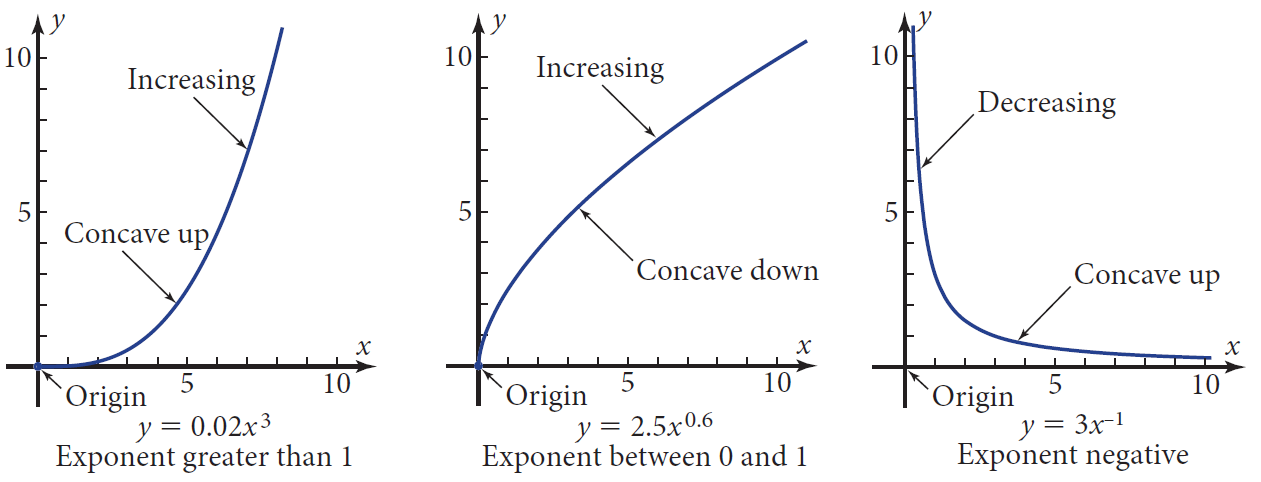
\includegraphics[width=1\textwidth]{figure/book3.png} % Adjust width here to scale the image
    \caption{Power functions}
\end{figure}

\begin{figure}[htbp]
    \centering
    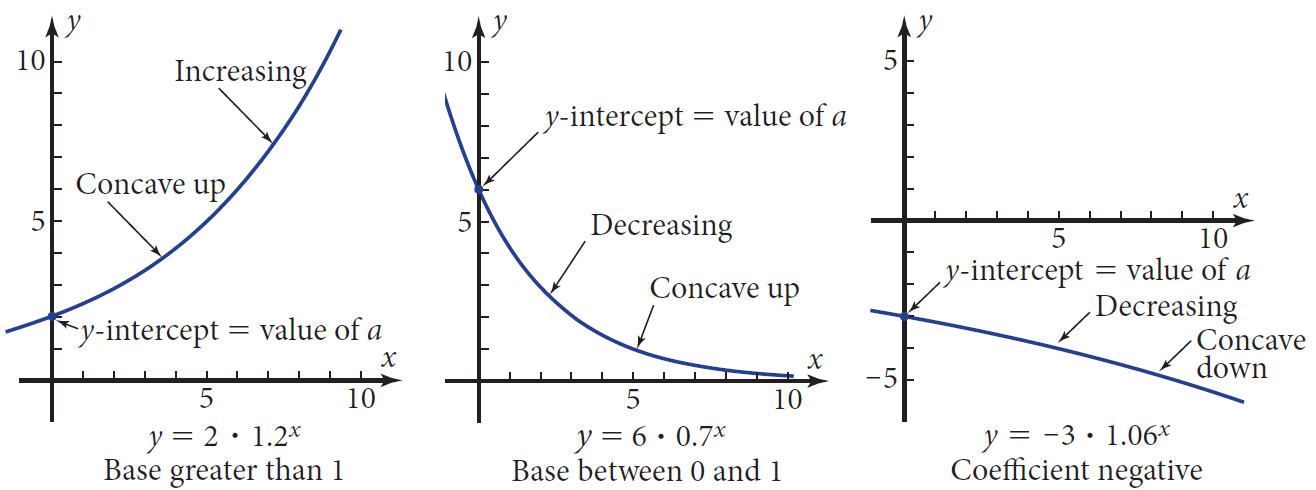
\includegraphics[width=1\textwidth]{figure/book4.png} % Adjust width here to scale the image
    \caption{Exponential functions}
\end{figure}

\begin{definition}{Base-10 Logarithms}

\[
\log x=y \iff 10^y=x
\]

\textit{Verbally}: $\log x$ is the exponent in the power of 10 that gives $x$   
\end{definition}

\begin{custombox}{Properties of base-10 logarithms}
\begin{itemize}
    \item Log of a Product:
    
    \[
    \log x y=\log x+\log y
    \]
    
    \textit{Verbally}: The $\log$ of a product equals the sum of the logs of the factors.
    \vspace{0.2cm}
    \item Log of a Quotient:
    
    \[
    \log \frac{x}{y}=\log x-\log y
    \]
    \vspace{0.1cm}
    \textit{Verbally}: The $\log$ of a quotient equals the log of the numerator minus the $\log$ of the denominator.
    \vspace{0.2cm}
    \item Log of a Power:
    \[
    \log x^y=y \log x
    \]
    \textit{Verbally}: The $\log$ of a power equals the exponent times the log of the base.
\end{itemize}

   
\end{custombox}

\begin{definition}{Common Logarithm and Natural Logarithm}
\hspace{1cm} \textit{Common}: The symbol $\log x$ means $\log _{10} x$.

\hspace{1cm}  \textit{Natural}: \hspace{0.2cm}The symbol $\ln x$ means $\log _e x$, where $e$ is a constant equal to $2.71828182845 \ldots$
\end{definition}

\begin{custombox}{The Change-of-Base Property of Logarithms}

\begin{equation*}
\log _a x=\frac{\log _b x}{\log _b a} \quad \text { or } \quad \log _a x=\frac{1}{\log _b a}\left(\log _b x\right)
\end{equation*}
    
\end{custombox}

\begin{custombox}{Properties of Logarithms}
\setlength{\leftskip}{1cm}  % Reset the text indent
\setlength{\rightskip}{1cm} % Reset the right indent
The Logarithm of a Power:
$$
\log _b x^y=y \log _b x
$$
The Logarithm of a Product:
$$
\log _b(x y)=\log _b x+\log _b y
$$
The Logarithm of a Quotient:
$$
\log _b \frac{x}{y}=\log _b x-\log _b y
$$
\setlength{\leftskip}{0cm}  % Reset the text indent
\setlength{\rightskip}{0cm} % Reset the right indent

\end{custombox}


% \chapter{Summation}\label{app:appendix01}

This appendix offers methods for evaluating summations, which occur frequently in the analysis of algorithms. Many
of the formulas here appear in any calculus text, but you will find it convenient to have these methods compiled in one place. The content of this appendix is based on the book \textit{Introduction to Algorithms}, (\cite{clrs4}). The Appendix is concluded with a useful cheat sheet for time complixity analysis.

When an algorithm contains an iterative control construct such as a \While or \For loop, you can express its running time as the sum of the times spent on each execution of the body of the loop. For example, in \autoref{sec:loop-analysis} we argued that the $i$'th iteration of $\proc{Quadratic-Sum}$ took time proportional to $i$ in the worst case. Adding up the time spent on each iteration produced the summation (or series) $\sum\limits_{i=1}^n i$. Evaluating this summation resulted in a bound of $\mathcal{O}(n^2)$ on the worst-case running time of the algorithm. This example illustrates why you should know how to manipulate summations. Before going into details, we provide an overview of the most important summations and their closed forms.

\begin{table}[htbp]
    \centering
    \renewcommand{\arraystretch}{2}
    \begin{tabular}{|c|c|}
    \hline
    \textbf{Sum} & \textbf{Closed Form} \\ \hline
    $\displaystyle \sum_{k=0}^n ar^k \, (r \neq 1)$ & $\displaystyle \frac{ar^{n+1} - a}{r - 1}$ \\ \hline
    $\displaystyle \sum_{k=1}^n k$ & $\displaystyle \frac{n(n+1)}{2}$ \\ \hline
    $\displaystyle \sum_{k=1}^n k^2$ & $\displaystyle \frac{n(n+1)(2n+1)}{6}$ \\ \hline
    $\displaystyle \sum_{k=1}^n k^3$ & $\displaystyle \frac{n^2(n+1)^2}{4}$ \\ \hline
    $\displaystyle \sum_{k=0}^n x^k \, (x \neq 1)$ & $\displaystyle \frac{x^{n+1} - 1}{x - 1}$ \\ \hline
    $\displaystyle \sum_{i=1,2,4,\ldots,n} i$ & $\displaystyle 2n - 1$ \\ \hline
    $\displaystyle \sum_{k=0}^\infty x^k, \, |x| < 1$ & $\displaystyle \frac{1}{1 - x}$ \\ \hline
    $\displaystyle \sum_{k=1}^\infty kx^{k-1}, \, |x| < 1$ & $\displaystyle \frac{1}{(1 - x)^2}$ \\ \hline
    $\displaystyle \sum_{k=1}^n \frac{1}{k}$ & $\displaystyle \ln n + O(1)$ \\ \hline
    $\displaystyle \sum_{k=1}^n (a + bk)$ & $\displaystyle a n + b \frac{n(n+1)}{2}$ \\ \hline  
    \end{tabular}
    \caption{Some Useful Summation Formulae}
\end{table}


\section*{Summation Notation}

Consider a sequence of numbers \( a_1, a_2, \ldots, a_n \), where \( n \) is a nonnegative integer. The sum of this sequence, \( a_1 + a_2 + \dots + a_n \), can be represented by the notation \( \sum_{k=1}^n a_k \). When \( n = 0 \), this summation is defined to have a value of 0. The result of a finite sum is always well-defined, and the order in which the terms are summed does not affect the final value.

For an infinite sequence \( a_1, a_2, \ldots \) of numbers, we represent their infinite sum \( a_1 + a_2 + \dots \) by the notation \( \sum_{k=1}^{\infty} a_k \), which corresponds to \( \lim_{n \rightarrow \infty} \sum_{k=1}^n a_k \). If this limit exists, the series is said to converge; otherwise, it diverges. Unlike finite sums, the terms of a convergent series cannot necessarily be rearranged without affecting the outcome. However, in an absolutely convergent series—one where \( \sum_{k=1}^{\infty} |a_k| \) also converges — the terms can be reordered without changing the sum.

\[
    \sum_{i=i_0}^n c a_i=c \sum_{i=i_0}^n a_i
\]

where $c$ is any number. So, we can factor constants out of a summation.

Similarly, we can split a summation into two summations:

\[
\sum_{i=i_0}^n\left(a_i \pm b_i\right)=\sum_{i=i_0}^n a_i \pm \sum_{i=i_0}^n b_i
\]

Note that we started the series at $i_0$ to denote the fact that they can start at any value of $i$ that we need them to. Also note that while we can break up sums and differences as we did above we can't do the same thing for products and quotients. In other words,

\[
    \sum_{i=i_0}^n\left(a_i b_i\right) \neq\left(\sum_{i=i_0}^n a_i\right)\left(\sum_{i=i_0}^n b_i\right) \qquad \text{and} \qquad \sum_{i=i_0}^n \frac{a_i}{b_i} \neq \frac{\sum_{i=i_0}^n a_i}{\sum_{i=i_0}^n b_i}.
\]

\section*{Linearity of Summation}
For any real number $c$ and any finite sequences $a_1, a_2, \ldots, a_n$ and $b_1, b_2, \ldots, b_n$,

\[
    \sum_{k=1}^n\left(c a_k+b_k\right)=c \sum_{k=1}^n a_k+\sum_{k=1}^n b_k .
\]

The linearity property also applies to infinite convergent series.

The linearity property applies to summations incorporating asymptotic notation. For example,

\[
    \sum_{k=1}^n \Theta(f(k))=\Theta\left(\sum_{k=1}^n f(k)\right) .
\]

In this equation, the $\Theta$-notation on the left-hand side applies to the variable $k$, but on the right-hand side, it applies to $n$. Such manipulations also apply to infinite convergent series.

\section*{Arithmetic Series}
The summation


\[
        \sum_{k=1}^n k=1+2+\cdots+n \label{eq:arithmetic-series}
\]

is an arithmetic series and has the value


\begin{align}
    \sum_{k=1}^n k & =\frac{n(n+1)}{2} \label{eq:sum-of-natural-numbers}  \\
    & =\Theta\left(n^2\right) . \label{eq:arithmetic-series-asymptotic}
\end{align}

A general arithmetic series includes an additive constant $a \geq 0$ and a constant coefficient $b>0$ in each term, but has the same total asymptotically:

\begin{equation}
    \sum_{k=1}^n(a+b k)=\Theta\left(n^2\right) . \label{eq:general-arithmetic-series}
    \end{equation}

\section*{Sums of Squares and Cubes}
The following formulas apply to summations of squares and cubes:

    \begin{equation}
    \sum_{k=0}^n k^2=\frac{n(n+1)(2 n+1)}{6}, \label{eq:sum-of-squares}
    \end{equation}

    \begin{equation}
        \sum_{k=0}^n k^3=\frac{n^2(n+1)^2}{4} . \label{eq:sum-of-cubes}
        \end{equation}

        \section*{Geometric Series}
        For real $x \neq 1$, the summation
        
        \[
            \sum_{k=0}^n x^k=1+x+x^2+\cdots+x^n
        \]
        
        is a geometric series and has the value
        
        \begin{equation}
            \sum_{k=0}^n x^k=\frac{x^{n+1}-1}{x-1} . \label{eq:geometric-series}
        \end{equation}
        
        The infinite decreasing geometric series occurs when the summation is infinite and $|x|<1$:
        
        \begin{equation}
            \sum_{k=0}^{\infty} x^k=\frac{1}{1-x} . \label{eq:infinite-geometric-series}
        \end{equation}
        
        If we assume that $0^0=1$, these formulas apply even when $x=0$.
        
        A \textbf{special} case of the geometric series arises when the terms form a progression of powers of 2. That is, the terms are \(1, 2, 4, 8, \ldots, n\). In this case:
        \[
            \sum_{i=1,2,4,\ldots,n} i = 1 + 2 + 4 + 8 + \cdots + n.
        \]
        
        This series can be derived from the general formula for a geometric series. The general form of a geometric series is:
        \[
            S = a + ar + ar^2 + \cdots + ar^{k-1},
        \]
        where:
        \begin{itemize}
            \item \(a\) is the first term (\(a=1\) in this case),
            \item \(r\) is the common ratio (\(r=2\) here),
            \item \(k\) is the number of terms in the series.
        \end{itemize}
        The number of terms, \(k\), is determined by how many times the progression \(1, 2, 4, \ldots, n\) doubles until reaching \(n\). Since \(n = 2^{k-1}\), we have \(k = \log_2(n) + 1\).
        
        Using the geometric series formula \eqref{eq:geometric-series}:
        \[
            \sum_{i=1,2,4,\ldots,n} i = \frac{2^k - 1}{2 - 1} = 2^k - 1.
        \]
        
        Substituting \(k = \log_2(n) + 1\):
        \[
            \sum_{i=1,2,4,\ldots,n} i = 2^{\log_2(n)+1} - 1 = 2n - 1.
        \]
        
        Thus, the sum of the powers of 2 up to \(n\) is:
        \[
            \sum_{i=1,2,4,\ldots,n} i = 2n - 1.
        \]
        

\section*{Harmonic Series}
For positive integers $n$, the $n$th harmonic number is

\begin{align}
    H_n & = 1 + \frac{1}{2} + \frac{1}{3} + \frac{1}{4} + \cdots + \frac{1}{n} \nonumber \\
        & = \sum_{k=1}^n \frac{1}{k} \label{eq:harmonic_sum} \\
        & = \ln n + O(1) . \label{eq:approximation}
\end{align}

\section*{Integrating and Differentiating}
Integrating or differentiating the formulas above yields additional formulas. For example, differentiating both sides of the infinite geometric series (\ref{eq:infinite-geometric-series}) and multiplying by $x$ gives


\begin{equation}
    \begin{aligned}
    & \sum_{k=0}^{\infty} k x^k=\frac{x}{(1-x)^2} \\ 
    & \text { for }|x|<1 . \label{eq:diff-geometric-series}
    \end{aligned}
\end{equation}

\section*{Telescoping Series}

For any sequence $a_0, a_1, \ldots, a_n$

\begin{equation}
    \sum_{k=1}^n\left(a_k-a_{k-1}\right)=a_n-a_0, \label{eq:telescoping-series}
\end{equation}

since each of the terms $a_1, a_2, \ldots, a_{n-1}$ is added in exactly once and subtracted out exactly once. We say that the sum telescopes. Similarly,

\[
    \sum_{k=0}^{n-1}\left(a_k-a_{k+1}\right)=a_0-a_n .
\]

As an example of a telescoping sum, consider the series

\[
\sum_{k=1}^{n-1} \frac{1}{k(k+1)}
\]

Rewriting each term as

\[
\frac{1}{k(k+1)}=\frac{1}{k}-\frac{1}{k+1},
\]

gives

\begin{align}
\sum_{k-1}^{n-1} \frac{1}{k(k+1)} & =\sum_{k-1}^{n-1}\left(\frac{1}{k}-\frac{1}{k+1}\right) \nonumber \\
& =1-\frac{1}{n} . \label{eq:telescoping-example}
\end{align}

\section*{Reindexing Sums}
A series can sometimes be simplified by changing its index, often reversing the order of summation. Consider the series $\sum_{k=0}^n a_{n-k}$. Because the terms in this summation are $a_n, a_{n-1}, \ldots, a_0$, we can reverse the order of indices by letting $j=n-k$ and rewrite this summation as

$$
\sum_{k=0}^n a_{n-k}=\sum_{l=0}^n a_j
$$


Generally, if the summation index appears in the body of the sum with a minus sign, it's worth thinking about reindexing.

As an example, consider the summation

\begin{equation}
    \sum_{k=1}^n \frac{1}{n-k+1} . \label{eq:reindexing-example}
\end{equation}


The index $k$ appears with a negative sign in $\dfrac{1}{(n-k+1)}$. And indeed, we can simplify this summation, this time setting $j=n-k+1$, yielding

\begin{equation}
    \sum_{k=1}^n \frac{1}{n-k+1}=\sum_{i=1}^n \frac{1}{j}, \label{eq:reindexing-example-solution} 
\end{equation}

which is just the harmonic series (\ref{eq:harmonic_sum}).

\section*{Products}
The finite product $a_1 a_2 \ldots a_n$ can be expressed as

\[
\prod_{k=1}^n a_k .
\]


If $n=0$, the value of the product is defined to be 1 . You can convert a formula with a product to a formula with a summation by using the identity

\[
\log \left(\prod_{k=1}^n a_k\right)=\sum_{k=1}^n \log a_k .
\]

\section*{Cheat Sheet for Time Complexity Analysis}

This section provides essential formulas and shortcuts for asymptotic analysis and algorithm evaluation. These complement the detailed summation methods in this appendix.

\begin{itemize}
    \item \textbf{Logarithmic Factorial Approximation (Stirling's Approximation):} 
    \[
    \log(n!) \approx n \log n - n.
    \]
 
    \item \textbf{Logarithmic Exponent Rule:} 
    \[
    2^{\log_2 n} = n.
    \]

    \item \textbf{Base as a Power with Logarithmic Exponent:} 
    If the base is \( a^b \) and the exponent involves \( \log_a \), then:
    \[
    (a^b)^{\log_a(n^c)} = n^{bc}.
    \]
    
    \textbf{Example:} \( 4^{\log_2(n^2)} = n^4 \) (since \( 4 = 2^2 \)).
    
    \item \textbf{Power of a Logarithm Rule:} 
    \[
    \log(n^k) = k \log n, \quad \text{for } k > 0.
    \]
    
    \item \textbf{Logarithmic Growth for Powers of 2:} 
    For \( n = 2^k \),
    \[
    k = \log_2 n.
    \]
    
    \item \textbf{Simplifying Logarithmic Expressions:} 
    \[
    \log_a n = \frac{\log_b n}{\log_b a}, \quad \text{for } a, b > 0.
    \]
    
    \item \textbf{Common Asymptotic Comparisons:} 
    \[
    n^c \ll c^n \quad \text{for any constant } c > 1.
    \]
    
    \item \textbf{Factorial Asymptotics (Expanded Stirling's Approximation):} 
    Using Stirling's formula, the growth of \( n! \) is approximately:
    \[
    n! = \Theta\left(\sqrt{2\pi n} \left(\frac{n}{e}\right)^n\right).
    \]
    
    \item \textbf{Sum of Powers of 2:} 
    If the terms in a series form powers of 2 (e.g., \( 1, 2, 4, 8, \ldots, n \)), the sum is:
    \[
    \sum_{i=1,2,4,\ldots,n} i = 2n - 1.
    \]

\end{itemize}


\end{document}

